\documentclass[]{book}
\usepackage{lmodern}
\usepackage{amssymb,amsmath}
\usepackage{ifxetex,ifluatex}
\usepackage{fixltx2e} % provides \textsubscript
\ifnum 0\ifxetex 1\fi\ifluatex 1\fi=0 % if pdftex
  \usepackage[T1]{fontenc}
  \usepackage[utf8]{inputenc}
\else % if luatex or xelatex
  \ifxetex
    \usepackage{mathspec}
  \else
    \usepackage{fontspec}
  \fi
  \defaultfontfeatures{Ligatures=TeX,Scale=MatchLowercase}
\fi
% use upquote if available, for straight quotes in verbatim environments
\IfFileExists{upquote.sty}{\usepackage{upquote}}{}
% use microtype if available
\IfFileExists{microtype.sty}{%
\usepackage{microtype}
\UseMicrotypeSet[protrusion]{basicmath} % disable protrusion for tt fonts
}{}
\usepackage[margin=1in]{geometry}
\usepackage{hyperref}
\hypersetup{unicode=true,
            pdftitle={Curso de R para meteorologia IAG/USP},
            pdfauthor={Sergio Ibarra-Espinosa, Amanda Rehbein, Daniel Schuch, e possivelmente outros (u r invited to collaborate)},
            pdfborder={0 0 0},
            breaklinks=true}
\urlstyle{same}  % don't use monospace font for urls
\usepackage{natbib}
\bibliographystyle{apalike}
\usepackage{color}
\usepackage{fancyvrb}
\newcommand{\VerbBar}{|}
\newcommand{\VERB}{\Verb[commandchars=\\\{\}]}
\DefineVerbatimEnvironment{Highlighting}{Verbatim}{commandchars=\\\{\}}
% Add ',fontsize=\small' for more characters per line
\usepackage{framed}
\definecolor{shadecolor}{RGB}{248,248,248}
\newenvironment{Shaded}{\begin{snugshade}}{\end{snugshade}}
\newcommand{\KeywordTok}[1]{\textcolor[rgb]{0.13,0.29,0.53}{\textbf{#1}}}
\newcommand{\DataTypeTok}[1]{\textcolor[rgb]{0.13,0.29,0.53}{#1}}
\newcommand{\DecValTok}[1]{\textcolor[rgb]{0.00,0.00,0.81}{#1}}
\newcommand{\BaseNTok}[1]{\textcolor[rgb]{0.00,0.00,0.81}{#1}}
\newcommand{\FloatTok}[1]{\textcolor[rgb]{0.00,0.00,0.81}{#1}}
\newcommand{\ConstantTok}[1]{\textcolor[rgb]{0.00,0.00,0.00}{#1}}
\newcommand{\CharTok}[1]{\textcolor[rgb]{0.31,0.60,0.02}{#1}}
\newcommand{\SpecialCharTok}[1]{\textcolor[rgb]{0.00,0.00,0.00}{#1}}
\newcommand{\StringTok}[1]{\textcolor[rgb]{0.31,0.60,0.02}{#1}}
\newcommand{\VerbatimStringTok}[1]{\textcolor[rgb]{0.31,0.60,0.02}{#1}}
\newcommand{\SpecialStringTok}[1]{\textcolor[rgb]{0.31,0.60,0.02}{#1}}
\newcommand{\ImportTok}[1]{#1}
\newcommand{\CommentTok}[1]{\textcolor[rgb]{0.56,0.35,0.01}{\textit{#1}}}
\newcommand{\DocumentationTok}[1]{\textcolor[rgb]{0.56,0.35,0.01}{\textbf{\textit{#1}}}}
\newcommand{\AnnotationTok}[1]{\textcolor[rgb]{0.56,0.35,0.01}{\textbf{\textit{#1}}}}
\newcommand{\CommentVarTok}[1]{\textcolor[rgb]{0.56,0.35,0.01}{\textbf{\textit{#1}}}}
\newcommand{\OtherTok}[1]{\textcolor[rgb]{0.56,0.35,0.01}{#1}}
\newcommand{\FunctionTok}[1]{\textcolor[rgb]{0.00,0.00,0.00}{#1}}
\newcommand{\VariableTok}[1]{\textcolor[rgb]{0.00,0.00,0.00}{#1}}
\newcommand{\ControlFlowTok}[1]{\textcolor[rgb]{0.13,0.29,0.53}{\textbf{#1}}}
\newcommand{\OperatorTok}[1]{\textcolor[rgb]{0.81,0.36,0.00}{\textbf{#1}}}
\newcommand{\BuiltInTok}[1]{#1}
\newcommand{\ExtensionTok}[1]{#1}
\newcommand{\PreprocessorTok}[1]{\textcolor[rgb]{0.56,0.35,0.01}{\textit{#1}}}
\newcommand{\AttributeTok}[1]{\textcolor[rgb]{0.77,0.63,0.00}{#1}}
\newcommand{\RegionMarkerTok}[1]{#1}
\newcommand{\InformationTok}[1]{\textcolor[rgb]{0.56,0.35,0.01}{\textbf{\textit{#1}}}}
\newcommand{\WarningTok}[1]{\textcolor[rgb]{0.56,0.35,0.01}{\textbf{\textit{#1}}}}
\newcommand{\AlertTok}[1]{\textcolor[rgb]{0.94,0.16,0.16}{#1}}
\newcommand{\ErrorTok}[1]{\textcolor[rgb]{0.64,0.00,0.00}{\textbf{#1}}}
\newcommand{\NormalTok}[1]{#1}
\usepackage{longtable,booktabs}
\usepackage{graphicx,grffile}
\makeatletter
\def\maxwidth{\ifdim\Gin@nat@width>\linewidth\linewidth\else\Gin@nat@width\fi}
\def\maxheight{\ifdim\Gin@nat@height>\textheight\textheight\else\Gin@nat@height\fi}
\makeatother
% Scale images if necessary, so that they will not overflow the page
% margins by default, and it is still possible to overwrite the defaults
% using explicit options in \includegraphics[width, height, ...]{}
\setkeys{Gin}{width=\maxwidth,height=\maxheight,keepaspectratio}
\IfFileExists{parskip.sty}{%
\usepackage{parskip}
}{% else
\setlength{\parindent}{0pt}
\setlength{\parskip}{6pt plus 2pt minus 1pt}
}
\setlength{\emergencystretch}{3em}  % prevent overfull lines
\providecommand{\tightlist}{%
  \setlength{\itemsep}{0pt}\setlength{\parskip}{0pt}}
\setcounter{secnumdepth}{5}
% Redefines (sub)paragraphs to behave more like sections
\ifx\paragraph\undefined\else
\let\oldparagraph\paragraph
\renewcommand{\paragraph}[1]{\oldparagraph{#1}\mbox{}}
\fi
\ifx\subparagraph\undefined\else
\let\oldsubparagraph\subparagraph
\renewcommand{\subparagraph}[1]{\oldsubparagraph{#1}\mbox{}}
\fi

%%% Use protect on footnotes to avoid problems with footnotes in titles
\let\rmarkdownfootnote\footnote%
\def\footnote{\protect\rmarkdownfootnote}

%%% Change title format to be more compact
\usepackage{titling}

% Create subtitle command for use in maketitle
\newcommand{\subtitle}[1]{
  \posttitle{
    \begin{center}\large#1\end{center}
    }
}

\setlength{\droptitle}{-2em}
  \title{Curso de R para meteorologia IAG/USP}
  \pretitle{\vspace{\droptitle}\centering\huge}
  \posttitle{\par}
  \author{Sergio Ibarra-Espinosa, Amanda Rehbein, Daniel Schuch, e possivelmente
outros (u r invited to collaborate)}
  \preauthor{\centering\large\emph}
  \postauthor{\par}
  \predate{\centering\large\emph}
  \postdate{\par}
  \date{2018-05-03}

\usepackage{booktabs}
\usepackage{amsthm}
\makeatletter
\def\thm@space@setup{%
  \thm@preskip=8pt plus 2pt minus 4pt
  \thm@postskip=\thm@preskip
}
\makeatother

\begin{document}
\maketitle

{
\setcounter{tocdepth}{1}
\tableofcontents
}
\chapter{Pre-requisitos do sistema}\label{primero}

Em Windows, instale além do R, Rtools
\url{https://cran.r-project.org/bin/windows/Rtools/}

Em MAC instale netcdf e:

\begin{Shaded}
\begin{Highlighting}[]
\ExtensionTok{brew}\NormalTok{ unlink gdal}
\ExtensionTok{brew}\NormalTok{ tap osgeo/osgeo4mac }\KeywordTok{&&} \ExtensionTok{brew}\NormalTok{ tap --repair}
\ExtensionTok{brew}\NormalTok{ install proj}
\ExtensionTok{brew}\NormalTok{ install geos}
\ExtensionTok{brew}\NormalTok{ install udunits}
\ExtensionTok{brew}\NormalTok{ install gdal2 --with-armadillo --with-complete --with-libkml --with-unsupported}
\ExtensionTok{brew}\NormalTok{ link --force gdal2}
\end{Highlighting}
\end{Shaded}

Em Ubuntu:

\begin{Shaded}
\begin{Highlighting}[]
  \ExtensionTok{-}\NormalTok{ sudo add-apt-repository ppa:ubuntugis/ubuntugis-unstable --yes}
  \ExtensionTok{-}\NormalTok{ sudo apt-get --yes --force-yes update -qq}
  \CommentTok{# install tmap dependencies}
  \ExtensionTok{-}\NormalTok{ sudo apt-get install --yes libprotobuf-dev protobuf-compiler libv8-3.14-dev}
  \CommentTok{# install tmap dependencies; for 16.04 libjq-dev this ppa is needed:}
  \ExtensionTok{-}\NormalTok{ sudo add-apt-repository -y ppa:opencpu/jq}
  \ExtensionTok{-}\NormalTok{ sudo apt-get --yes --force-yes update -qq}
  \ExtensionTok{-}\NormalTok{ sudo apt-get install libjq-dev}
  \CommentTok{# units/udunits2 dependency:}
  \ExtensionTok{-}\NormalTok{ sudo apt-get install --yes libudunits2-dev}
  \CommentTok{# sf dependencies:}
  \ExtensionTok{-}\NormalTok{ sudo apt-get install --yes libproj-dev libgeos-dev libgdal-dev libnetcdf-dev  netcdf-bin gdal-bin}
\end{Highlighting}
\end{Shaded}

\section{Pacotes usados neste curso}\label{pacotes-usados-neste-curso}

Para fazer este curso instale os seguintes pacotes como indicado:

\begin{Shaded}
\begin{Highlighting}[]
\KeywordTok{install.packages}\NormalTok{(}\StringTok{"devtools"}\NormalTok{)}
\NormalTok{devtools}\OperatorTok{::}\KeywordTok{install_github}\NormalTok{(}\StringTok{"tidyverse/tidyverse"}\NormalTok{)}
\NormalTok{devtools}\OperatorTok{::}\KeywordTok{install_github}\NormalTok{(}\StringTok{"r-spatial/sf"}\NormalTok{)}
\NormalTok{devtools}\OperatorTok{::}\KeywordTok{install_github}\NormalTok{(}\StringTok{"r-spatial/mapview"}\NormalTok{)}
\NormalTok{devtools}\OperatorTok{::}\KeywordTok{install_github}\NormalTok{(}\StringTok{"r-spatial/stars"}\NormalTok{)}
\KeywordTok{install.packages}\NormalTok{(}\KeywordTok{c}\NormalTok{(}\StringTok{"raster"}\NormalTok{, }\StringTok{"sp"}\NormalTok{, }\StringTok{"rgdal"}\NormalTok{, }\StringTok{"maptools"}\NormalTok{, }\StringTok{"ncdf4"}\NormalTok{))}
\KeywordTok{install.packages}\NormalTok{(}\KeywordTok{c}\NormalTok{(}\StringTok{"cptcity"}\NormalTok{, }\StringTok{"data.table"}\NormalTok{, }\StringTok{"openair"}\NormalTok{))}
\end{Highlighting}
\end{Shaded}

\begin{itemize}
\tightlist
\item
  \href{https://CRAN.R-project.org/package=devtools}{devtools} é um
  pacote para instalar pacotes de diferentes repositórios
\item
  \href{https://github.com/tidyverse}{tidyverse} é o universo de pacotes
  do Hadley Wickham. A instalação tem que ser usando devtools, pois
  precisamos plotar os objetos espacias sf usando
  \href{https://www.isgeomsfinggplot2yet.site/}{geom\_sf}.
\item
  \href{https://github.com/r-spatial/sf}{sf} e
  \href{https://github.com/r-spatial/mapbiew}{mapview},
  \href{https://github.com/r-spatial/stars}{stars}, raster, sp, rgdal e
  maptools são para a parte espacial. Lembrar que os objetos em
  meteorologias são espaço-temporais.
\item
  ncdf4 é um pacote para manipular arquivos NetCDF.
\item
  \href{https://ibarraespinosa.github.io/cptcity/}{cptcity} é um pacote
  que tem 7140 paletas de cores do arquivo web cpt-city
  (\url{http://soliton.vm.bytemark.co.uk/pub/cpt-city/index.html}).
\item
  \href{http://davidcarslaw.github.io/openair/}{openair} é um pacote
  para trabalhar com dados de qualidade do ar e meteorologia.
\end{itemize}

Se faltarem dependencias de sistema, instale elas e instale os pacotes.

\section{Colaborar}\label{colaborar}

A forma preferida de colaboração é com pull-requests em
\url{https://github.com/ibarraespinosa/cursoR/pull/new/master}. Lembre
de aplicar a Guia de Estilo de R de Google
(\url{https://google.github.io/styleguide/Rguide.xml}) ou com o formato
de formatR \url{https://yihui.name/formatr/}. Em poucas palavras, lembre
que seu código vai ser lido por seres humanos. Se quiser tem acesso no
repositório deste curso, me contate. Tem um botão para editar qualquer
página.

\section{Aportar com dados}\label{aportar-com-dados}

Se você tem dados para fazer este curso mais legal, por favor, edite
este aquivo e com pull request, eu vou fazer um merge para poder.

\begin{enumerate}
\def\labelenumi{\arabic{enumi}.}
\item
  NCEP: \url{ftp://nomads.ncdc.noaa.gov/GFS/analysis_only/}
\item
\item
\end{enumerate}

\chapter{Intro}\label{intro}

Este curso é para pos, então vamos ver conteúdo rapidamente e se não da
tempo, este curso esta online no sitio
\url{https://github.com/atmoschem/cursorIAG}.

Eu tento usar
\href{http://stat.ethz.ch/R-manual/R-devel/library/base/html/00Index.html}{BASE}
sempre que posso, e se não da ai vou para outros paradigmas.

Outros pacotes de BASE:
\href{http://stat.ethz.ch/R-manual/R-devel/library/utils/html/00Index.html}{utils},
\href{http://stat.ethz.ch/R-manual/R-devel/library/stats/html/00Index.html}{stats},
\href{http://stat.ethz.ch/R-manual/R-devel/library/datasets/html/00Index.html}{datasets},
\href{http://stat.ethz.ch/R-manual/R-devel/library/graphics/html/00Index.html}{graphics},
\href{https://stat.ethz.ch/R-manual/R-devel/library/grDevices/html/00Index.html}{grDevices},
\href{https://stat.ethz.ch/R-manual/R-devel/library/grid/html/00Index.html}{grid},
\href{https://stat.ethz.ch/R-manual/R-devel/library/methods/html/00Index.html}{methods},
\href{https://stat.ethz.ch/R-manual/R-devel/library/tools/html/00Index.html}{tools},
\href{https://stat.ethz.ch/R-manual/R-devel/library/parallel/html/00Index.html}{parallel},
\href{https://stat.ethz.ch/R-manual/R-devel/library/compiler/html/00Index.html}{compiler},
\href{https://stat.ethz.ch/R-manual/R-devel/library/splines/html/00Index.html}{splines},
\href{https://stat.ethz.ch/R-manual/R-devel/library/tcltk/html/00Index.html}{tcltk}
,
\href{https://stat.ethz.ch/R-manual/R-devel/library/stats4/html/00Index.html}{stats4}.

Veja
\href{https://cran.r-project.org/web/packages/available_packages_by_name.html}{outros}
pacotes.

Este curso esta baseado no livro
\href{https://leanpub.com/rprogramming}{R Programming for Data Science}.

Vamos usar \href{https://www.rstudio.com/}{Rstudio}

\textbf{Dica:}

\begin{itemize}
\tightlist
\item
  Se não sabe como usar uma função, escreva: \texttt{?função}.
\item
  As funções tem argumentos, use \textbf{TAB} para ver eles numa função.
\end{itemize}

\section{IMPORTANTE}\label{importante}

teu novo melhor amigo, besti friendi, BFF, parceiro, mano, tabarish,
komrade, compaheiro, colega, buisiness partner amd whatever meanningful
is

\begin{itemize}
\tightlist
\item
  \textbf{TAB} no \textbf{RSTUDIO}.
\end{itemize}

Esta combinação é tão boa, como o cafe com leite, pizza e abacaxi,
vitamina de acabate com amendoim Manaus, a melhor combinação.


\includegraphics[width=5.88in]{figuras/tab-key-}

Porque quando se tu não lembra os argumentos da função, e não quer ver o
help \emph{?} de cada função, so clica \textbf{TAB} e RSTUDIO te
mostrara a lista de argumentos.

Vamos lá!

\chapter{R!}\label{r}

\begin{itemize}
\tightlist
\item
  Quase em qualquer sistema operacional mas eu vou focar em Linux.
\item
  Muita documentação:
\item
  \href{http://cran.r-project.org/doc/manuals/r-release/R-intro.html}{Intro}.
\item
  \href{http://cran.r-project.org/doc/manuals/r-release/R-data.html}{I/O}.
\item
  Quer fazer um pacote?
  \href{http://cran.r-project.org/doc/manuals/r-release/R-exts.html}{Veja},
  \href{http://cran.r-project.org/doc/manuals/r-release/R-ints.html}{aqui}
  e
  \href{http://cran.r-project.org/doc/manuals/r-release/R-lang.html}{aqui}.
\item
  \href{https://stackoverflow.com/questions/tagged/r}{Stackoverflow}
  provides a great source of resources.
\end{itemize}

\section{Objetos de R}\label{objetos-de-r}

\begin{itemize}
\tightlist
\item
  Character a
\item
  numeric 1
\item
  integer 1
\item
  complex 0+1i
\item
  logical TRUE
\end{itemize}

\section{Classe}\label{classe}

\texttt{class} função permite ver a classe dos objetos

\section{Vetores}\label{vetores}

\begin{itemize}
\tightlist
\item
  c(``A'', ``C'', ``D'')
\item
  1:5 = c(1, 2, 3, 4, 5)
\item
  c(TRUE, FALSE)
\item
  c(1i, -1i)
\item
  c(1, ``C'', ``D'') qual é a classe???
\item
  c(1, NA, ``D'') qual é a classe???
\item
  c(1, NA, NaN) qual é a classe???
\end{itemize}

\section{\texorpdfstring{Convertir objetos com
\texttt{as}}{Convertir objetos com as}}\label{convertir-objetos-com-as}

\begin{Shaded}
\begin{Highlighting}[]
\KeywordTok{as.numeric}\NormalTok{(}\KeywordTok{c}\NormalTok{(}\DecValTok{1}\NormalTok{, }\StringTok{"C"}\NormalTok{, }\StringTok{"D"}\NormalTok{))}
\end{Highlighting}
\end{Shaded}

\begin{verbatim}
## Warning: NAs introduzidos por coerção
\end{verbatim}

\begin{verbatim}
## [1]  1 NA NA
\end{verbatim}

\section{\texorpdfstring{Matrices e a função
\texttt{matrix}}{Matrices e a função matrix}}\label{matrices-e-a-funcao-matrix}

\textbf{{[}linhas, colunas{]}}

\begin{itemize}
\tightlist
\item
  permitidos elementos \textbf{da mesma clase}!
\end{itemize}

vamos ver os argumentos da função \texttt{matrix}

\begin{Shaded}
\begin{Highlighting}[]
\KeywordTok{args}\NormalTok{(matrix)}
\end{Highlighting}
\end{Shaded}

\begin{verbatim}
## function (data = NA, nrow = 1, ncol = 1, byrow = FALSE, dimnames = NULL) 
## NULL
\end{verbatim}

usando TAB

\begin{Shaded}
\begin{Highlighting}[]
\NormalTok{(m <-}\StringTok{ }\KeywordTok{matrix}\NormalTok{(}\DataTypeTok{data =} \DecValTok{0}\NormalTok{, }\DataTypeTok{nrow =} \DecValTok{4}\NormalTok{, }\DataTypeTok{ncol =} \DecValTok{4}\NormalTok{))}
\end{Highlighting}
\end{Shaded}

\begin{verbatim}
##      [,1] [,2] [,3] [,4]
## [1,]    0    0    0    0
## [2,]    0    0    0    0
## [3,]    0    0    0    0
## [4,]    0    0    0    0
\end{verbatim}

\begin{Shaded}
\begin{Highlighting}[]
\NormalTok{(m1 <-}\StringTok{ }\KeywordTok{matrix}\NormalTok{(}\DataTypeTok{data =} \DecValTok{1}\OperatorTok{:}\NormalTok{(}\DecValTok{4}\OperatorTok{*}\DecValTok{4}\NormalTok{), }\DataTypeTok{nrow =} \DecValTok{4}\NormalTok{, }\DataTypeTok{ncol =} \DecValTok{4}\NormalTok{))}
\end{Highlighting}
\end{Shaded}

\begin{verbatim}
##      [,1] [,2] [,3] [,4]
## [1,]    1    5    9   13
## [2,]    2    6   10   14
## [3,]    3    7   11   15
## [4,]    4    8   12   16
\end{verbatim}

\begin{Shaded}
\begin{Highlighting}[]
\KeywordTok{dim}\NormalTok{(m1)}
\end{Highlighting}
\end{Shaded}

\begin{verbatim}
## [1] 4 4
\end{verbatim}

\begin{Shaded}
\begin{Highlighting}[]
\NormalTok{(m2 <-}\StringTok{ }\KeywordTok{matrix}\NormalTok{(}\DataTypeTok{data =} \DecValTok{1}\OperatorTok{:}\NormalTok{(}\DecValTok{4}\OperatorTok{*}\DecValTok{4}\NormalTok{), }\DataTypeTok{nrow =} \DecValTok{4}\NormalTok{, }\DataTypeTok{ncol =} \DecValTok{4}\NormalTok{, }\DataTypeTok{byrow =} \OtherTok{TRUE}\NormalTok{))}
\end{Highlighting}
\end{Shaded}

\begin{verbatim}
##      [,1] [,2] [,3] [,4]
## [1,]    1    2    3    4
## [2,]    5    6    7    8
## [3,]    9   10   11   12
## [4,]   13   14   15   16
\end{verbatim}

\section{Array}\label{array}

É como uma matriz de matrizes de matrizes de matrizes\ldots{}\ldots{}
and so on.

\begin{Shaded}
\begin{Highlighting}[]
\KeywordTok{args}\NormalTok{(array)}
\end{Highlighting}
\end{Shaded}

\begin{verbatim}
## function (data = NA, dim = length(data), dimnames = NULL) 
## NULL
\end{verbatim}

lembre usar TAB

\begin{Shaded}
\begin{Highlighting}[]
\NormalTok{(a <-}\StringTok{ }\KeywordTok{array}\NormalTok{(}\DataTypeTok{data =} \DecValTok{0}\NormalTok{, }\DataTypeTok{dim =} \KeywordTok{c}\NormalTok{(}\DecValTok{1}\NormalTok{,}\DecValTok{1}\NormalTok{)))}
\end{Highlighting}
\end{Shaded}

\begin{verbatim}
##      [,1]
## [1,]    0
\end{verbatim}

\begin{Shaded}
\begin{Highlighting}[]
\KeywordTok{class}\NormalTok{(a)}
\end{Highlighting}
\end{Shaded}

\begin{verbatim}
## [1] "matrix"
\end{verbatim}

\begin{Shaded}
\begin{Highlighting}[]
\NormalTok{(a <-}\StringTok{ }\KeywordTok{array}\NormalTok{(}\DataTypeTok{data =} \DecValTok{0}\NormalTok{, }\DataTypeTok{dim =} \KeywordTok{c}\NormalTok{(}\DecValTok{1}\NormalTok{,}\DecValTok{1}\NormalTok{,}\DecValTok{1}\NormalTok{)))}
\end{Highlighting}
\end{Shaded}

\begin{verbatim}
## , , 1
## 
##      [,1]
## [1,]    0
\end{verbatim}

\begin{Shaded}
\begin{Highlighting}[]
\KeywordTok{class}\NormalTok{(a)}
\end{Highlighting}
\end{Shaded}

\begin{verbatim}
## [1] "array"
\end{verbatim}

\begin{Shaded}
\begin{Highlighting}[]
\NormalTok{(a <-}\StringTok{ }\KeywordTok{array}\NormalTok{(}\DataTypeTok{data =} \DecValTok{0}\NormalTok{, }\DataTypeTok{dim =} \KeywordTok{c}\NormalTok{(}\DecValTok{2}\NormalTok{,}\DecValTok{2}\NormalTok{,}\DecValTok{2}\NormalTok{)))}
\end{Highlighting}
\end{Shaded}

\begin{verbatim}
## , , 1
## 
##      [,1] [,2]
## [1,]    0    0
## [2,]    0    0
## 
## , , 2
## 
##      [,1] [,2]
## [1,]    0    0
## [2,]    0    0
\end{verbatim}

\begin{Shaded}
\begin{Highlighting}[]
\NormalTok{(a <-}\StringTok{ }\KeywordTok{array}\NormalTok{(}\DataTypeTok{data =} \DecValTok{0}\NormalTok{, }\DataTypeTok{dim =} \KeywordTok{c}\NormalTok{(}\DecValTok{2}\NormalTok{,}\DecValTok{4}\NormalTok{,}\DecValTok{4}\NormalTok{)))}
\end{Highlighting}
\end{Shaded}

\begin{verbatim}
## , , 1
## 
##      [,1] [,2] [,3] [,4]
## [1,]    0    0    0    0
## [2,]    0    0    0    0
## 
## , , 2
## 
##      [,1] [,2] [,3] [,4]
## [1,]    0    0    0    0
## [2,]    0    0    0    0
## 
## , , 3
## 
##      [,1] [,2] [,3] [,4]
## [1,]    0    0    0    0
## [2,]    0    0    0    0
## 
## , , 4
## 
##      [,1] [,2] [,3] [,4]
## [1,]    0    0    0    0
## [2,]    0    0    0    0
\end{verbatim}

\begin{Shaded}
\begin{Highlighting}[]
\KeywordTok{dim}\NormalTok{(a)}
\end{Highlighting}
\end{Shaded}

\begin{verbatim}
## [1] 2 4 4
\end{verbatim}

\begin{Shaded}
\begin{Highlighting}[]
\NormalTok{(a <-}\StringTok{ }\KeywordTok{array}\NormalTok{(}\DataTypeTok{data =} \DecValTok{0}\NormalTok{, }\DataTypeTok{dim =} \KeywordTok{c}\NormalTok{(}\DecValTok{2}\NormalTok{, }\DecValTok{2}\NormalTok{,}\DecValTok{2}\NormalTok{,}\DecValTok{2}\NormalTok{)))}
\end{Highlighting}
\end{Shaded}

\section{\texorpdfstring{\texttt{list}}{list}}\label{list}

As listas são como sacolas, e dentro delas, tu pode colocar mais
sacolas\ldots{} então, tu pode ter sacolas, dentro de sacolas, dentro de
sacolas\ldots{} ou

\begin{Shaded}
\begin{Highlighting}[]
\KeywordTok{list}\NormalTok{(}\KeywordTok{list}\NormalTok{(}\KeywordTok{list}\NormalTok{(}\KeywordTok{list}\NormalTok{(}\DecValTok{1}\NormalTok{))))}
\end{Highlighting}
\end{Shaded}

\begin{verbatim}
## [[1]]
## [[1]][[1]]
## [[1]][[1]][[1]]
## [[1]][[1]][[1]][[1]]
## [1] 1
\end{verbatim}

a diferença das matrices, tu pode colocar cualquer coisa nas listas, por
exemplo: funções, characters, etc.

\begin{Shaded}
\begin{Highlighting}[]
\NormalTok{(x <-}\StringTok{ }\KeywordTok{list}\NormalTok{(}\DecValTok{1}\NormalTok{, }\StringTok{"a"}\NormalTok{, }\OtherTok{TRUE}\NormalTok{, }\DecValTok{1} \OperatorTok{+}\StringTok{ }\NormalTok{4i))}
\end{Highlighting}
\end{Shaded}

\begin{verbatim}
## [[1]]
## [1] 1
## 
## [[2]]
## [1] "a"
## 
## [[3]]
## [1] TRUE
## 
## [[4]]
## [1] 1+4i
\end{verbatim}

\section{Tempo e Data}\label{tempo-e-data}

R tem classes de tempo e data:

\begin{Shaded}
\begin{Highlighting}[]
\NormalTok{(a <-}\StringTok{ }\KeywordTok{ISOdate}\NormalTok{(}\DataTypeTok{year =} \DecValTok{2018}\NormalTok{, }\DataTypeTok{month =} \DecValTok{4}\NormalTok{, }\DataTypeTok{day =} \DecValTok{5}\NormalTok{))}
\end{Highlighting}
\end{Shaded}

\begin{verbatim}
## [1] "2018-04-05 12:00:00 GMT"
\end{verbatim}

\begin{Shaded}
\begin{Highlighting}[]
\KeywordTok{class}\NormalTok{(a)}
\end{Highlighting}
\end{Shaded}

\begin{verbatim}
## [1] "POSIXct" "POSIXt"
\end{verbatim}

\begin{Shaded}
\begin{Highlighting}[]
\NormalTok{(b <-}\StringTok{ }\KeywordTok{ISOdate}\NormalTok{(}\DataTypeTok{year =} \DecValTok{2018}\NormalTok{, }\DataTypeTok{month =} \DecValTok{4}\NormalTok{, }\DataTypeTok{day =} \DecValTok{5}\NormalTok{, }\DataTypeTok{tz =} \StringTok{"Americas/Sao_Paulo"}\NormalTok{))}
\end{Highlighting}
\end{Shaded}

\begin{verbatim}
## [1] "2018-04-05 12:00:00 Americas"
\end{verbatim}

tempo

\begin{Shaded}
\begin{Highlighting}[]
\NormalTok{(d <-}\StringTok{ }\KeywordTok{ISOdatetime}\NormalTok{(}\DataTypeTok{year =} \DecValTok{2018}\NormalTok{, }\DataTypeTok{month =} \DecValTok{4}\NormalTok{, }\DataTypeTok{day =} \DecValTok{5}\NormalTok{, }\DataTypeTok{hour =} \DecValTok{0}\NormalTok{, }\DataTypeTok{min =} \DecValTok{0}\NormalTok{, }\DataTypeTok{sec =} \DecValTok{0}\NormalTok{,}
                  \DataTypeTok{tz =} \StringTok{"Americas/Sao_Paulo"}\NormalTok{))}
\end{Highlighting}
\end{Shaded}

\begin{verbatim}
## [1] "2018-04-05 Americas"
\end{verbatim}

O pacote \href{https://github.com/eddelbuettel/nanotime}{nanotime}
permite trabalhar com nano segundos.

Da pra fazer secuencias:

\begin{Shaded}
\begin{Highlighting}[]
\NormalTok{hoje <-}\StringTok{ }\KeywordTok{Sys.time}\NormalTok{()}
\NormalTok{(a <-}\StringTok{ }\KeywordTok{seq.POSIXt}\NormalTok{(}\DataTypeTok{from =}\NormalTok{ hoje, }\DataTypeTok{by =} \DecValTok{3600}\NormalTok{, }\DataTypeTok{length.out =} \DecValTok{24}\NormalTok{))}
\end{Highlighting}
\end{Shaded}

\begin{verbatim}
##  [1] "2018-05-03 23:39:07 -03" "2018-05-04 00:39:07 -03"
##  [3] "2018-05-04 01:39:07 -03" "2018-05-04 02:39:07 -03"
##  [5] "2018-05-04 03:39:07 -03" "2018-05-04 04:39:07 -03"
##  [7] "2018-05-04 05:39:07 -03" "2018-05-04 06:39:07 -03"
##  [9] "2018-05-04 07:39:07 -03" "2018-05-04 08:39:07 -03"
## [11] "2018-05-04 09:39:07 -03" "2018-05-04 10:39:07 -03"
## [13] "2018-05-04 11:39:07 -03" "2018-05-04 12:39:07 -03"
## [15] "2018-05-04 13:39:07 -03" "2018-05-04 14:39:07 -03"
## [17] "2018-05-04 15:39:07 -03" "2018-05-04 16:39:07 -03"
## [19] "2018-05-04 17:39:07 -03" "2018-05-04 18:39:07 -03"
## [21] "2018-05-04 19:39:07 -03" "2018-05-04 20:39:07 -03"
## [23] "2018-05-04 21:39:07 -03" "2018-05-04 22:39:07 -03"
\end{verbatim}

funções bacana: \textbf{weekdays}, \textbf{month}, \textbf{julian}

\begin{Shaded}
\begin{Highlighting}[]
\KeywordTok{weekdays}\NormalTok{(a)}
\end{Highlighting}
\end{Shaded}

\begin{verbatim}
##  [1] "quinta" "sexta"  "sexta"  "sexta"  "sexta"  "sexta"  "sexta" 
##  [8] "sexta"  "sexta"  "sexta"  "sexta"  "sexta"  "sexta"  "sexta" 
## [15] "sexta"  "sexta"  "sexta"  "sexta"  "sexta"  "sexta"  "sexta" 
## [22] "sexta"  "sexta"  "sexta"
\end{verbatim}

\begin{Shaded}
\begin{Highlighting}[]
\KeywordTok{months}\NormalTok{(a)}
\end{Highlighting}
\end{Shaded}

\begin{verbatim}
##  [1] "maio" "maio" "maio" "maio" "maio" "maio" "maio" "maio" "maio" "maio"
## [11] "maio" "maio" "maio" "maio" "maio" "maio" "maio" "maio" "maio" "maio"
## [21] "maio" "maio" "maio" "maio"
\end{verbatim}

\begin{Shaded}
\begin{Highlighting}[]
\KeywordTok{julian}\NormalTok{(a) }\CommentTok{#olha ?julian... dias desde origin}
\end{Highlighting}
\end{Shaded}

\begin{verbatim}
## Time differences in days
##  [1] 17655.11 17655.15 17655.19 17655.24 17655.28 17655.32 17655.36
##  [8] 17655.40 17655.44 17655.49 17655.53 17655.57 17655.61 17655.65
## [15] 17655.69 17655.74 17655.78 17655.82 17655.86 17655.90 17655.94
## [22] 17655.99 17656.03 17656.07
## attr(,"origin")
## [1] "1970-01-01 GMT"
\end{verbatim}

olha \url{https://en.wikipedia.org/wiki/Julian_day}:

\section{Fatores}\label{fatores}

Os \texttt{factors} podem ser um pouco infernais. Olha
\href{http://www.burns-stat.com/documents/books/the-r-inferno/}{R
INFERNO}

Usados para representar categorias, ejemplo clasico para nos, dias da
semana.

\begin{Shaded}
\begin{Highlighting}[]
\NormalTok{a <-}\StringTok{ }\KeywordTok{seq.POSIXt}\NormalTok{(}\DataTypeTok{from =}\NormalTok{ hoje, }\DataTypeTok{by =} \DecValTok{3600}\NormalTok{, }\DataTypeTok{length.out =} \DecValTok{24}\OperatorTok{*}\DecValTok{7}\NormalTok{)}
\NormalTok{aa <-}\StringTok{ }\KeywordTok{weekdays}\NormalTok{(a)}
\KeywordTok{class}\NormalTok{(aa)}
\end{Highlighting}
\end{Shaded}

\begin{verbatim}
## [1] "character"
\end{verbatim}

\begin{Shaded}
\begin{Highlighting}[]
\KeywordTok{factor}\NormalTok{(aa)}
\end{Highlighting}
\end{Shaded}

\begin{verbatim}
##   [1] quinta  sexta   sexta   sexta   sexta   sexta   sexta   sexta  
##   [9] sexta   sexta   sexta   sexta   sexta   sexta   sexta   sexta  
##  [17] sexta   sexta   sexta   sexta   sexta   sexta   sexta   sexta  
##  [25] sexta   sábado  sábado  sábado  sábado  sábado  sábado  sábado 
##  [33] sábado  sábado  sábado  sábado  sábado  sábado  sábado  sábado 
##  [41] sábado  sábado  sábado  sábado  sábado  sábado  sábado  sábado 
##  [49] sábado  domingo domingo domingo domingo domingo domingo domingo
##  [57] domingo domingo domingo domingo domingo domingo domingo domingo
##  [65] domingo domingo domingo domingo domingo domingo domingo domingo
##  [73] domingo segunda segunda segunda segunda segunda segunda segunda
##  [81] segunda segunda segunda segunda segunda segunda segunda segunda
##  [89] segunda segunda segunda segunda segunda segunda segunda segunda
##  [97] segunda terça   terça   terça   terça   terça   terça   terça  
## [105] terça   terça   terça   terça   terça   terça   terça   terça  
## [113] terça   terça   terça   terça   terça   terça   terça   terça  
## [121] terça   quarta  quarta  quarta  quarta  quarta  quarta  quarta 
## [129] quarta  quarta  quarta  quarta  quarta  quarta  quarta  quarta 
## [137] quarta  quarta  quarta  quarta  quarta  quarta  quarta  quarta 
## [145] quarta  quinta  quinta  quinta  quinta  quinta  quinta  quinta 
## [153] quinta  quinta  quinta  quinta  quinta  quinta  quinta  quinta 
## [161] quinta  quinta  quinta  quinta  quinta  quinta  quinta  quinta 
## Levels: domingo quarta quinta sábado segunda sexta terça
\end{verbatim}

olha os \textbf{Levels}

Então:

\begin{Shaded}
\begin{Highlighting}[]
\NormalTok{ab <-}\StringTok{ }\KeywordTok{factor}\NormalTok{(}\DataTypeTok{x =}\NormalTok{ aa,}
             \DataTypeTok{levels =} \KeywordTok{c}\NormalTok{(}\StringTok{"Monday"}\NormalTok{, }\StringTok{"Tuesday"}\NormalTok{,  }\StringTok{"Wednesday"}\NormalTok{,  }\StringTok{"Thursday"}\NormalTok{,}
                        \StringTok{"Friday"}\NormalTok{, }\StringTok{"Saturday"}\NormalTok{, }\StringTok{"Sunday"}\NormalTok{))}
\KeywordTok{levels}\NormalTok{(ab)}
\end{Highlighting}
\end{Shaded}

\begin{verbatim}
## [1] "Monday"    "Tuesday"   "Wednesday" "Thursday"  "Friday"    "Saturday" 
## [7] "Sunday"
\end{verbatim}

\section{\texorpdfstring{\texttt{data.frames}}{data.frames}}\label{data.frames}

\emph{lembre ?data.frame}

São como planilha EXCEL\ldots{}. mais o menos

É uma classe bem especial, tem elementos de matriz mas o modo é lista

\begin{Shaded}
\begin{Highlighting}[]
\NormalTok{(df <-}\StringTok{ }\KeywordTok{data.frame}\NormalTok{(}\DataTypeTok{a =} \DecValTok{1}\OperatorTok{:}\DecValTok{3}\NormalTok{))}
\end{Highlighting}
\end{Shaded}

\begin{verbatim}
##   a
## 1 1
## 2 2
## 3 3
\end{verbatim}

\begin{Shaded}
\begin{Highlighting}[]
\KeywordTok{names}\NormalTok{(df)}
\end{Highlighting}
\end{Shaded}

\begin{verbatim}
## [1] "a"
\end{verbatim}

\begin{Shaded}
\begin{Highlighting}[]
\KeywordTok{class}\NormalTok{(df)}
\end{Highlighting}
\end{Shaded}

\begin{verbatim}
## [1] "data.frame"
\end{verbatim}

\begin{Shaded}
\begin{Highlighting}[]
\KeywordTok{mode}\NormalTok{(df)}
\end{Highlighting}
\end{Shaded}

\begin{verbatim}
## [1] "list"
\end{verbatim}

Então

\begin{Shaded}
\begin{Highlighting}[]
\KeywordTok{nrow}\NormalTok{(df)}
\end{Highlighting}
\end{Shaded}

\begin{verbatim}
## [1] 3
\end{verbatim}

\begin{Shaded}
\begin{Highlighting}[]
\KeywordTok{ncol}\NormalTok{(df)}
\end{Highlighting}
\end{Shaded}

\begin{verbatim}
## [1] 1
\end{verbatim}

\begin{Shaded}
\begin{Highlighting}[]
\KeywordTok{dim}\NormalTok{(df)}
\end{Highlighting}
\end{Shaded}

\begin{verbatim}
## [1] 3 1
\end{verbatim}

\chapter{Importando e exportando dados em
R}\label{importando-e-exportando-dados-em-r}

\section{data-frames}\label{data-frames}

Probabelmente um dos promeiros objetos que vamos usar quando começamos
usar R. Pensa num data-frame como uma planilha de Libreoffice (o excel).
Os data-frame pode ser criaos como foi visto na seção anterior. O
principal, é que temos varias funções para ler data-frames no R, entre
elas

\begin{itemize}
\tightlist
\item
  read.csv
\item
  read.csv2
\item
  read.table
\end{itemize}

Agora vamos a ler dados do repositorio usando read.table, mas primeiro
vamos lembrar que se tu precisar ver a ajuda da função, tem que escrever
no R \texttt{?read.table}. Então, agora vamos ver os argumentos da
função:

\begin{Shaded}
\begin{Highlighting}[]
\KeywordTok{args}\NormalTok{(read.table)}
\end{Highlighting}
\end{Shaded}

\begin{verbatim}
## function (file, header = FALSE, sep = "", quote = "\"'", dec = ".", 
##     numerals = c("allow.loss", "warn.loss", "no.loss"), row.names, 
##     col.names, as.is = !stringsAsFactors, na.strings = "NA", 
##     colClasses = NA, nrows = -1, skip = 0, check.names = TRUE, 
##     fill = !blank.lines.skip, strip.white = FALSE, blank.lines.skip = TRUE, 
##     comment.char = "#", allowEscapes = FALSE, flush = FALSE, 
##     stringsAsFactors = default.stringsAsFactors(), fileEncoding = "", 
##     encoding = "unknown", text, skipNul = FALSE) 
## NULL
\end{verbatim}

Aqui vem-se os valores default dos argumentos da função
\texttt{read.table}. O terceiro argumento é sep, com valores por default
= ``''.

\begin{Shaded}
\begin{Highlighting}[]
\NormalTok{df <-}\StringTok{ }\KeywordTok{read.table}\NormalTok{(}\StringTok{"https://raw.githubusercontent.com/ibarraespinosa/cursoR/master/dados/NOXIPEN2014.txt"}\NormalTok{)}
\end{Highlighting}
\end{Shaded}

Agora vamos usar a funções \texttt{head} and \texttt{tail} para ver as
primeiras e as ultimas 6 linhas do data-frame.

\begin{Shaded}
\begin{Highlighting}[]
\KeywordTok{head}\NormalTok{(df)}
\end{Highlighting}
\end{Shaded}

\begin{verbatim}
##   TipodeRede TipodeMonitoramento            Tipo       Data  Hora
## 2 Automático              CETESB Dados Primários 01/01/2014 01:00
## 3 Automático              CETESB Dados Primários 01/01/2014 02:00
## 4 Automático              CETESB Dados Primários 01/01/2014 03:00
## 5 Automático              CETESB Dados Primários 01/01/2014 04:00
## 6 Automático              CETESB Dados Primários 01/01/2014 05:00
## 7 Automático              CETESB Dados Primários 01/01/2014 06:00
##   CodigoEstação                NomeEstação              NomeParâmetro
## 2            95 Cid.Universitária-USP-Ipen NOx (Óxidos de Nitrogênio)
## 3            95 Cid.Universitária-USP-Ipen NOx (Óxidos de Nitrogênio)
## 4            95 Cid.Universitária-USP-Ipen NOx (Óxidos de Nitrogênio)
## 5            95 Cid.Universitária-USP-Ipen NOx (Óxidos de Nitrogênio)
## 6            95 Cid.Universitária-USP-Ipen NOx (Óxidos de Nitrogênio)
## 7            95 Cid.Universitária-USP-Ipen NOx (Óxidos de Nitrogênio)
##   UnidadedeMedida MediaHoraria MediaMovel Valido
## 2             ppb            9          -    Não
## 3             ppb            9          -    Sim
## 4             ppb            5          -    Sim
## 5             ppb            4          -    Sim
## 6             ppb            5          -    Sim
## 7             ppb            5          -    Sim
\end{verbatim}

\begin{Shaded}
\begin{Highlighting}[]
\KeywordTok{tail}\NormalTok{(df)}
\end{Highlighting}
\end{Shaded}

\begin{verbatim}
##      TipodeRede TipodeMonitoramento            Tipo       Data  Hora
## 8577 Automático              CETESB Dados Primários 01/01/2015 19:00
## 8578 Automático              CETESB Dados Primários 01/01/2015 20:00
## 8579 Automático              CETESB Dados Primários 01/01/2015 21:00
## 8580 Automático              CETESB Dados Primários 01/01/2015 22:00
## 8581 Automático              CETESB Dados Primários 01/01/2015 23:00
## 8582 Automático              CETESB Dados Primários 01/01/2015 24:00
##      CodigoEstação                NomeEstação              NomeParâmetro
## 8577            95 Cid.Universitária-USP-Ipen NOx (Óxidos de Nitrogênio)
## 8578            95 Cid.Universitária-USP-Ipen NOx (Óxidos de Nitrogênio)
## 8579            95 Cid.Universitária-USP-Ipen NOx (Óxidos de Nitrogênio)
## 8580            95 Cid.Universitária-USP-Ipen NOx (Óxidos de Nitrogênio)
## 8581            95 Cid.Universitária-USP-Ipen NOx (Óxidos de Nitrogênio)
## 8582            95 Cid.Universitária-USP-Ipen NOx (Óxidos de Nitrogênio)
##      UnidadedeMedida MediaHoraria MediaMovel Valido
## 8577             ppb            3          -    Sim
## 8578             ppb            8          -    Sim
## 8579             ppb           11          -    Sim
## 8580             ppb           11          -    Sim
## 8581             ppb           16          -    Sim
## 8582             ppb           NA          -    Sim
\end{verbatim}

Agora vamos ler os mesmos dados com outro formato e testar e read.table
funciona do mesmo jeito

\begin{Shaded}
\begin{Highlighting}[]
\NormalTok{df2 <-}\StringTok{ }\KeywordTok{read.table}\NormalTok{(}\StringTok{"https://raw.githubusercontent.com/ibarraespinosa/cursoR/master/dados/NOXIPEN2014v2.txt"}\NormalTok{)}
\CommentTok{# Error in scan(file = file, what = what, sep = sep, quote = quote, dec = dec, : }
\CommentTok{# linha 1 não tinha 6 elementos}
\end{Highlighting}
\end{Shaded}

Vemos a mensagem de error, mas o que quer dizer.

\textbf{Se tu recever um banco de dados tipo .txt e quer abrir no
R\ldots{} ABRE ELE COM BLOCO DE NOTAS PRIMEIRO!!!}

O primeiro arquivo:

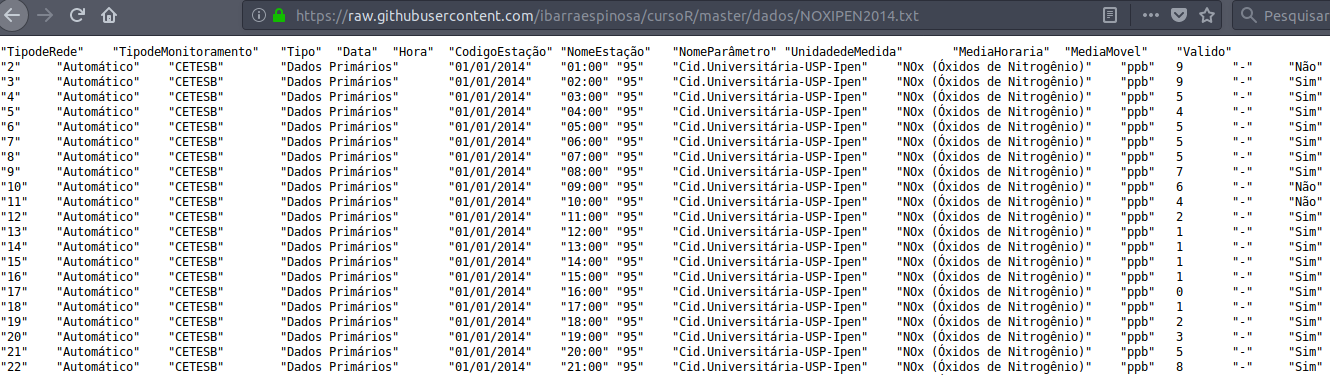
\includegraphics[width=18.47in]{figuras/f1}

O segundo arquivo é:

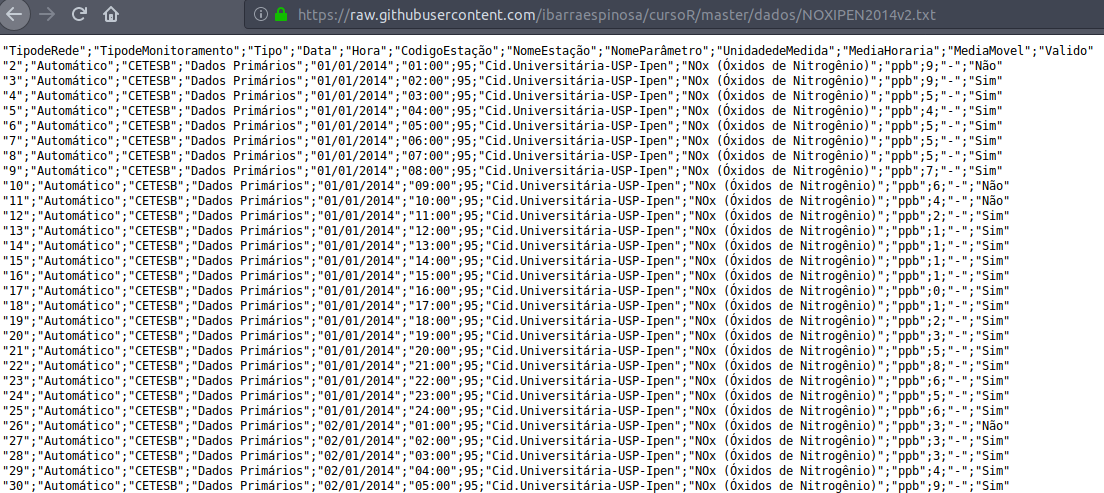
\includegraphics[width=15.33in]{figuras/f2}

qual é a diferença?

Como vemos o segundo arquivo tem separação de ``;'', entao, temos que
lero arquivo assim:

\begin{Shaded}
\begin{Highlighting}[]
\NormalTok{df2 <-}\StringTok{ }\KeywordTok{read.table}\NormalTok{(}\StringTok{"https://raw.githubusercontent.com/ibarraespinosa/cursoR/master/dados/NOXIPEN2014v2.txt"}\NormalTok{, }\DataTypeTok{sep =} \StringTok{";"}\NormalTok{)}
\KeywordTok{head}\NormalTok{(df2)}
\end{Highlighting}
\end{Shaded}

\begin{verbatim}
##   TipodeRede TipodeMonitoramento            Tipo       Data  Hora
## 2 Automático              CETESB Dados Primários 01/01/2014 01:00
## 3 Automático              CETESB Dados Primários 01/01/2014 02:00
## 4 Automático              CETESB Dados Primários 01/01/2014 03:00
## 5 Automático              CETESB Dados Primários 01/01/2014 04:00
## 6 Automático              CETESB Dados Primários 01/01/2014 05:00
## 7 Automático              CETESB Dados Primários 01/01/2014 06:00
##   CodigoEstação                NomeEstação              NomeParâmetro
## 2            95 Cid.Universitária-USP-Ipen NOx (Óxidos de Nitrogênio)
## 3            95 Cid.Universitária-USP-Ipen NOx (Óxidos de Nitrogênio)
## 4            95 Cid.Universitária-USP-Ipen NOx (Óxidos de Nitrogênio)
## 5            95 Cid.Universitária-USP-Ipen NOx (Óxidos de Nitrogênio)
## 6            95 Cid.Universitária-USP-Ipen NOx (Óxidos de Nitrogênio)
## 7            95 Cid.Universitária-USP-Ipen NOx (Óxidos de Nitrogênio)
##   UnidadedeMedida MediaHoraria MediaMovel Valido
## 2             ppb            9          -    Não
## 3             ppb            9          -    Sim
## 4             ppb            5          -    Sim
## 5             ppb            4          -    Sim
## 6             ppb            5          -    Sim
## 7             ppb            5          -    Sim
\end{verbatim}

\begin{Shaded}
\begin{Highlighting}[]
\KeywordTok{tail}\NormalTok{(df2)}
\end{Highlighting}
\end{Shaded}

\begin{verbatim}
##      TipodeRede TipodeMonitoramento            Tipo       Data  Hora
## 8577 Automático              CETESB Dados Primários 01/01/2015 19:00
## 8578 Automático              CETESB Dados Primários 01/01/2015 20:00
## 8579 Automático              CETESB Dados Primários 01/01/2015 21:00
## 8580 Automático              CETESB Dados Primários 01/01/2015 22:00
## 8581 Automático              CETESB Dados Primários 01/01/2015 23:00
## 8582 Automático              CETESB Dados Primários 01/01/2015 24:00
##      CodigoEstação                NomeEstação              NomeParâmetro
## 8577            95 Cid.Universitária-USP-Ipen NOx (Óxidos de Nitrogênio)
## 8578            95 Cid.Universitária-USP-Ipen NOx (Óxidos de Nitrogênio)
## 8579            95 Cid.Universitária-USP-Ipen NOx (Óxidos de Nitrogênio)
## 8580            95 Cid.Universitária-USP-Ipen NOx (Óxidos de Nitrogênio)
## 8581            95 Cid.Universitária-USP-Ipen NOx (Óxidos de Nitrogênio)
## 8582            95 Cid.Universitária-USP-Ipen NOx (Óxidos de Nitrogênio)
##      UnidadedeMedida MediaHoraria MediaMovel Valido
## 8577             ppb            3          -    Sim
## 8578             ppb            8          -    Sim
## 8579             ppb           11          -    Sim
## 8580             ppb           11          -    Sim
## 8581             ppb           16          -    Sim
## 8582             ppb           NA          -    Sim
\end{verbatim}

\subsection{Qua dificultades tu já enfrentou importando
dados?}\label{qua-dificultades-tu-ja-enfrentou-importando-dados}

\section{\texorpdfstring{Exportando texto com
\texttt{write.table}}{Exportando texto com write.table}}\label{exportando-texto-com-write.table}

Exportar é bem facil, mas se sabemos os argumentos das funções, vai ser
mais eficiente ainda. Vamos \texttt{write.table}

\begin{Shaded}
\begin{Highlighting}[]
\KeywordTok{args}\NormalTok{(write.table)}
\end{Highlighting}
\end{Shaded}

\begin{verbatim}
## function (x, file = "", append = FALSE, quote = TRUE, sep = " ", 
##     eol = "\n", na = "NA", dec = ".", row.names = TRUE, col.names = TRUE, 
##     qmethod = c("escape", "double"), fileEncoding = "") 
## NULL
\end{verbatim}

Se temos um data-frame com colunas de classe character,
\texttt{quote\ =\ TRUE} quer dizer que o arquivo de texto resultante vai
ter aspas nas colunas de caracter.

\texttt{sep} é como vão ser separadas as colunas. Se tu quer abrir o
arquivo com Excel, poderia separar com ``,'', ``;'', " ``,''\t``\ldots{}
Depende como tu quer.

eol quer dizer \emph{end of line}, e é para ver a forma de colocar o
``end of line''

\textbf{row.names}.. esta TRUE mas SEMPRE SEMPRE SEMPRE COLOCA:

\textbf{row.names = FALSE}. Se não, R vai adiiconar uma coluna com os
indices das linhas\ldots{}.

col.names se tu quer o nome nas colunas\ldots{}

\textbf{PRATICA!}

\section{\texorpdfstring{Exportando objetos com
\texttt{save}}{Exportando objetos com save}}\label{exportando-objetos-com-save}

\begin{Shaded}
\begin{Highlighting}[]
\KeywordTok{args}\NormalTok{(save)}
\end{Highlighting}
\end{Shaded}

\begin{verbatim}
## function (..., list = character(), file = stop("'file' must be specified"), 
##     ascii = FALSE, version = NULL, envir = parent.frame(), compress = isTRUE(!ascii), 
##     compression_level, eval.promises = TRUE, precheck = TRUE) 
## NULL
\end{verbatim}

\texttt{save} salva o objeto com a extensão .rda. Para carregar de volta
o objeto, tem que ser feito com a função \texttt{load}

\begin{Shaded}
\begin{Highlighting}[]
\KeywordTok{args}\NormalTok{(load)}
\end{Highlighting}
\end{Shaded}

\begin{verbatim}
## function (file, envir = parent.frame(), verbose = FALSE) 
## NULL
\end{verbatim}

O que pode ser ruim, porque as vezes tu esqueceu o nome do objeto no
ambiente de R. Por exemplo, tu salvou o arquivo

\begin{Shaded}
\begin{Highlighting}[]
\KeywordTok{save}\NormalTok{(frenteFria, }\DataTypeTok{file =} \StringTok{"FrenteQuente.rda"}\NormalTok{)}
\end{Highlighting}
\end{Shaded}

logo tu carrega

\begin{Shaded}
\begin{Highlighting}[]
\KeywordTok{load}\NormalTok{(}\StringTok{"FrenteQuente.rda"}\NormalTok{)}
\end{Highlighting}
\end{Shaded}

acreditando que vai ter tua frente quente, mas o nome do objeto no
ambiente de R é frenteDria\ldots{} então, tem que ficar de olho, e como
somos imperfeito, vai dar merda\ldots{}.

O melhor da função é que permite salvar com tipos de compressão, por
exemplo compress = ``xz''.

\section{\texorpdfstring{Exportando objetos com
\texttt{saveRDS}}{Exportando objetos com saveRDS}}\label{exportando-objetos-com-saverds}

Esta é uma das minhas funçoes favoritas no R

\begin{Shaded}
\begin{Highlighting}[]
\KeywordTok{args}\NormalTok{(saveRDS)}
\end{Highlighting}
\end{Shaded}

\begin{verbatim}
## function (object, file = "", ascii = FALSE, version = NULL, compress = TRUE, 
##     refhook = NULL) 
## NULL
\end{verbatim}

e

\begin{Shaded}
\begin{Highlighting}[]
\KeywordTok{args}\NormalTok{(readRDS)}
\end{Highlighting}
\end{Shaded}

\begin{verbatim}
## function (file, refhook = NULL) 
## NULL
\end{verbatim}

Tu consegue salvar o objeto R de forma serializada e compactada com o
argumento \texttt{compress} mas o melhor é quando vai chamar o objeto de
volta ao R. Agora tu usa o \texttt{readRDS} e coloca o nome que tu
quiser.

\begin{Shaded}
\begin{Highlighting}[]
\KeywordTok{saveRDS}\NormalTok{(FrenteQuente, }\StringTok{"FrenteQuente.rds"}\NormalTok{)}
\end{Highlighting}
\end{Shaded}

\begin{Shaded}
\begin{Highlighting}[]
\NormalTok{frenteQ <-}\StringTok{ }\KeywordTok{readRDS}\NormalTok{(}\StringTok{"FremteQuente.rds"}\NormalTok{)}
\end{Highlighting}
\end{Shaded}

\section{Processando nossa
data-frame}\label{processando-nossa-data-frame}

Tem numeroas formas e pacotes para ordenar, arrangiar (Arrange), mutar e
cambiar as data-frames. As mais conhecidas são provablemente do universe
\emph{tidyverse} com o famoso pacote \emph{dplyr}. Mas, nesta curso
vamos focar em \textbf{base}.

Vamos então revisar a classe de cada columna do nosso data-frame com a
função \texttt{sapply}, apresentada em outro capitulo, mas se quiser, da
uma olhada em \texttt{?sapply}.

\begin{Shaded}
\begin{Highlighting}[]
\KeywordTok{sapply}\NormalTok{(df, class)}
\end{Highlighting}
\end{Shaded}

\begin{verbatim}
##          TipodeRede TipodeMonitoramento                Tipo 
##            "factor"            "factor"            "factor" 
##                Data                Hora       CodigoEstação 
##            "factor"            "factor"           "integer" 
##         NomeEstação       NomeParâmetro     UnidadedeMedida 
##            "factor"            "factor"            "factor" 
##        MediaHoraria          MediaMovel              Valido 
##           "integer"            "factor"            "factor"
\end{verbatim}

Quando nos trabalhamos com series de tempo, é importante ter a variabel
de tempo reconhecida como ``tempo'', especificamente como classe
``POSIXct''. Mas, a classe de Data é ``factor'' e de Hora tambem
``factor'', o que é ruim. Então, vamos criar uma variabel de tempo mais
standard com formato 2018-05-03 23:39:11.

Para isso temos que grudar as variabel Data e Hora. Faremios isso numa
nova varaibel chamada tempo\_char, adicionando ela diretamente no
\texttt{df} com o cifrão DOLLAR \$. O grude pode ser feito com as
funções \texttt{paste} ou \texttt{paste0}.

\begin{Shaded}
\begin{Highlighting}[]
\NormalTok{df}\OperatorTok{$}\NormalTok{tempo_char <-}\StringTok{ }\KeywordTok{paste}\NormalTok{(df}\OperatorTok{$}\NormalTok{Data, df}\OperatorTok{$}\NormalTok{Hora)}
\KeywordTok{head}\NormalTok{(df}\OperatorTok{$}\NormalTok{tempo_char)}
\end{Highlighting}
\end{Shaded}

\begin{verbatim}
## [1] "01/01/2014 01:00" "01/01/2014 02:00" "01/01/2014 03:00"
## [4] "01/01/2014 04:00" "01/01/2014 05:00" "01/01/2014 06:00"
\end{verbatim}

\begin{Shaded}
\begin{Highlighting}[]
\KeywordTok{class}\NormalTok{(df}\OperatorTok{$}\NormalTok{tempo_char)}
\end{Highlighting}
\end{Shaded}

\begin{verbatim}
## [1] "character"
\end{verbatim}

Esta melhorando mas ainda tem clase character.

Para convertir a nossa classe POSIXct podemos usar a função
\texttt{as.POSIXct} (olha \texttt{as.POSIXct}). Seus argumentos são:

\begin{Shaded}
\begin{Highlighting}[]
\KeywordTok{args}\NormalTok{(as.POSIXct)}
\end{Highlighting}
\end{Shaded}

\begin{verbatim}
## function (x, tz = "", ...) 
## NULL
\end{verbatim}

Então, vamos criar outra variabel tempo o formato POSIXct

\begin{Shaded}
\begin{Highlighting}[]
\NormalTok{df}\OperatorTok{$}\NormalTok{tempo <-}\StringTok{ }\KeywordTok{as.POSIXct}\NormalTok{(}\DataTypeTok{x =}\NormalTok{ df}\OperatorTok{$}\NormalTok{tempo_char, }\DataTypeTok{tz =} \StringTok{"Americas/Sao_Paulo"}\NormalTok{, }
                       \DataTypeTok{format =} \StringTok{"%d/%m/%Y %H:%M"}\NormalTok{)}
\KeywordTok{head}\NormalTok{(df}\OperatorTok{$}\NormalTok{tempo)}
\end{Highlighting}
\end{Shaded}

\begin{verbatim}
## [1] "2014-01-01 01:00:00 Americas" "2014-01-01 02:00:00 Americas"
## [3] "2014-01-01 03:00:00 Americas" "2014-01-01 04:00:00 Americas"
## [5] "2014-01-01 05:00:00 Americas" "2014-01-01 06:00:00 Americas"
\end{verbatim}

\begin{Shaded}
\begin{Highlighting}[]
\KeywordTok{class}\NormalTok{(df}\OperatorTok{$}\NormalTok{tempo)}
\end{Highlighting}
\end{Shaded}

\begin{verbatim}
## [1] "POSIXct" "POSIXt"
\end{verbatim}

Agora, vamos a extraer os dias da semana do tempo, mes e dia juliano:

\begin{Shaded}
\begin{Highlighting}[]
\NormalTok{df}\OperatorTok{$}\NormalTok{weekdays <-}\StringTok{ }\KeywordTok{format}\NormalTok{(df}\OperatorTok{$}\NormalTok{tempo, }\StringTok{"%A"}\NormalTok{)}
\KeywordTok{head}\NormalTok{(df}\OperatorTok{$}\NormalTok{weekdays)}
\end{Highlighting}
\end{Shaded}

\begin{verbatim}
## [1] "quarta" "quarta" "quarta" "quarta" "quarta" "quarta"
\end{verbatim}

\begin{Shaded}
\begin{Highlighting}[]
\NormalTok{df}\OperatorTok{$}\NormalTok{mes <-}\StringTok{ }\KeywordTok{format}\NormalTok{(df}\OperatorTok{$}\NormalTok{tempo, }\StringTok{"%B"}\NormalTok{)}
\KeywordTok{head}\NormalTok{(df}\OperatorTok{$}\NormalTok{mes)}
\end{Highlighting}
\end{Shaded}

\begin{verbatim}
## [1] "janeiro" "janeiro" "janeiro" "janeiro" "janeiro" "janeiro"
\end{verbatim}

\begin{Shaded}
\begin{Highlighting}[]
\NormalTok{df}\OperatorTok{$}\NormalTok{diajuliano <-}\StringTok{ }\KeywordTok{julian}\NormalTok{(df}\OperatorTok{$}\NormalTok{tempo)}
\KeywordTok{head}\NormalTok{(df}\OperatorTok{$}\NormalTok{diajuliano)}
\end{Highlighting}
\end{Shaded}

\begin{verbatim}
## Time differences in days
## [1] 16071.04 16071.08 16071.12 16071.17 16071.21 16071.25
\end{verbatim}

\begin{Shaded}
\begin{Highlighting}[]
\NormalTok{df}\OperatorTok{$}\NormalTok{ano <-}\StringTok{ }\KeywordTok{format}\NormalTok{(df}\OperatorTok{$}\NormalTok{tempo, }\StringTok{"%Y"}\NormalTok{)}
\end{Highlighting}
\end{Shaded}

\section{aggregate}\label{aggregate}

Vamos a carregar a nossa data.frame. Primero uma olhada

\begin{Shaded}
\begin{Highlighting}[]
\KeywordTok{head}\NormalTok{(df)}
\end{Highlighting}
\end{Shaded}

\begin{verbatim}
##   TipodeRede TipodeMonitoramento            Tipo       Data  Hora
## 2 Automático              CETESB Dados Primários 01/01/2014 01:00
## 3 Automático              CETESB Dados Primários 01/01/2014 02:00
## 4 Automático              CETESB Dados Primários 01/01/2014 03:00
## 5 Automático              CETESB Dados Primários 01/01/2014 04:00
## 6 Automático              CETESB Dados Primários 01/01/2014 05:00
## 7 Automático              CETESB Dados Primários 01/01/2014 06:00
##   CodigoEstação                NomeEstação              NomeParâmetro
## 2            95 Cid.Universitária-USP-Ipen NOx (Óxidos de Nitrogênio)
## 3            95 Cid.Universitária-USP-Ipen NOx (Óxidos de Nitrogênio)
## 4            95 Cid.Universitária-USP-Ipen NOx (Óxidos de Nitrogênio)
## 5            95 Cid.Universitária-USP-Ipen NOx (Óxidos de Nitrogênio)
## 6            95 Cid.Universitária-USP-Ipen NOx (Óxidos de Nitrogênio)
## 7            95 Cid.Universitária-USP-Ipen NOx (Óxidos de Nitrogênio)
##   UnidadedeMedida MediaHoraria MediaMovel Valido       tempo_char
## 2             ppb            9          -    Não 01/01/2014 01:00
## 3             ppb            9          -    Sim 01/01/2014 02:00
## 4             ppb            5          -    Sim 01/01/2014 03:00
## 5             ppb            4          -    Sim 01/01/2014 04:00
## 6             ppb            5          -    Sim 01/01/2014 05:00
## 7             ppb            5          -    Sim 01/01/2014 06:00
##                 tempo weekdays     mes    diajuliano  ano
## 2 2014-01-01 01:00:00   quarta janeiro 16071.04 days 2014
## 3 2014-01-01 02:00:00   quarta janeiro 16071.08 days 2014
## 4 2014-01-01 03:00:00   quarta janeiro 16071.12 days 2014
## 5 2014-01-01 04:00:00   quarta janeiro 16071.17 days 2014
## 6 2014-01-01 05:00:00   quarta janeiro 16071.21 days 2014
## 7 2014-01-01 06:00:00   quarta janeiro 16071.25 days 2014
\end{verbatim}

Poderiamos calcular a media horaria por dia da semana. Então:

\begin{Shaded}
\begin{Highlighting}[]
\NormalTok{dff <-}\StringTok{ }\KeywordTok{aggregate}\NormalTok{(df}\OperatorTok{$}\NormalTok{MediaHoraria, }\DataTypeTok{by =} \KeywordTok{list}\NormalTok{(df}\OperatorTok{$}\NormalTok{weekdays), sum, }\DataTypeTok{na.rm =}\NormalTok{ T)}
\NormalTok{dff}
\end{Highlighting}
\end{Shaded}

\begin{verbatim}
##   Group.1     x
## 1 domingo 20327
## 2  quarta 40180
## 3  quinta 41199
## 4  sábado 32298
## 5 segunda 34057
## 6   sexta 42558
## 7   terça 37904
\end{verbatim}

\begin{Shaded}
\begin{Highlighting}[]
\KeywordTok{names}\NormalTok{(dff) <-}\StringTok{ }\KeywordTok{c}\NormalTok{(}\StringTok{"dias"}\NormalTok{, }\StringTok{"MediaHoraria"}\NormalTok{)}
\end{Highlighting}
\end{Shaded}

\begin{Shaded}
\begin{Highlighting}[]
\NormalTok{dff}\OperatorTok{$}\NormalTok{sd <-}\StringTok{ }\KeywordTok{aggregate}\NormalTok{(df}\OperatorTok{$}\NormalTok{MediaHoraria, }
                    \DataTypeTok{by =} \KeywordTok{list}\NormalTok{(df}\OperatorTok{$}\NormalTok{weekdays), }
\NormalTok{                    sum, }\DataTypeTok{na.rm =}\NormalTok{ T)}\OperatorTok{$}\NormalTok{x}
\NormalTok{dff}
\end{Highlighting}
\end{Shaded}

\begin{verbatim}
##      dias MediaHoraria    sd
## 1 domingo        20327 20327
## 2  quarta        40180 40180
## 3  quinta        41199 41199
## 4  sábado        32298 32298
## 5 segunda        34057 34057
## 6   sexta        42558 42558
## 7   terça        37904 37904
\end{verbatim}

\section{subset}\label{subset}

Como poderiamos escolher só o mes de janeiro??

\begin{Shaded}
\begin{Highlighting}[]
\CommentTok{#[     LINHAS    ,  COLUNAS   ]}
\NormalTok{df[df}\OperatorTok{$}\NormalTok{mes }\OperatorTok{==}\StringTok{ "janeiro"}\NormalTok{, ] }\CommentTok{#TODAS AS COLUNAS}
\end{Highlighting}
\end{Shaded}

\begin{verbatim}
##      TipodeRede TipodeMonitoramento            Tipo       Data  Hora
## 2    Automático              CETESB Dados Primários 01/01/2014 01:00
## 3    Automático              CETESB Dados Primários 01/01/2014 02:00
## 4    Automático              CETESB Dados Primários 01/01/2014 03:00
## 5    Automático              CETESB Dados Primários 01/01/2014 04:00
## 6    Automático              CETESB Dados Primários 01/01/2014 05:00
## 7    Automático              CETESB Dados Primários 01/01/2014 06:00
## 8    Automático              CETESB Dados Primários 01/01/2014 07:00
## 9    Automático              CETESB Dados Primários 01/01/2014 08:00
## 10   Automático              CETESB Dados Primários 01/01/2014 09:00
## 11   Automático              CETESB Dados Primários 01/01/2014 10:00
## 12   Automático              CETESB Dados Primários 01/01/2014 11:00
## 13   Automático              CETESB Dados Primários 01/01/2014 12:00
## 14   Automático              CETESB Dados Primários 01/01/2014 13:00
## 15   Automático              CETESB Dados Primários 01/01/2014 14:00
## 16   Automático              CETESB Dados Primários 01/01/2014 15:00
## 17   Automático              CETESB Dados Primários 01/01/2014 16:00
## 18   Automático              CETESB Dados Primários 01/01/2014 17:00
## 19   Automático              CETESB Dados Primários 01/01/2014 18:00
## 20   Automático              CETESB Dados Primários 01/01/2014 19:00
## 21   Automático              CETESB Dados Primários 01/01/2014 20:00
## 22   Automático              CETESB Dados Primários 01/01/2014 21:00
## 23   Automático              CETESB Dados Primários 01/01/2014 22:00
## 24   Automático              CETESB Dados Primários 01/01/2014 23:00
## 25   Automático              CETESB Dados Primários 01/01/2014 24:00
## 26   Automático              CETESB Dados Primários 02/01/2014 01:00
## 27   Automático              CETESB Dados Primários 02/01/2014 02:00
## 28   Automático              CETESB Dados Primários 02/01/2014 03:00
## 29   Automático              CETESB Dados Primários 02/01/2014 04:00
## 30   Automático              CETESB Dados Primários 02/01/2014 05:00
## 31   Automático              CETESB Dados Primários 02/01/2014 06:00
## 32   Automático              CETESB Dados Primários 02/01/2014 07:00
## 33   Automático              CETESB Dados Primários 02/01/2014 08:00
## 34   Automático              CETESB Dados Primários 02/01/2014 09:00
## 35   Automático              CETESB Dados Primários 02/01/2014 10:00
## 36   Automático              CETESB Dados Primários 02/01/2014 11:00
## 37   Automático              CETESB Dados Primários 02/01/2014 12:00
## 38   Automático              CETESB Dados Primários 02/01/2014 13:00
## 39   Automático              CETESB Dados Primários 02/01/2014 14:00
## 40   Automático              CETESB Dados Primários 02/01/2014 15:00
## 41   Automático              CETESB Dados Primários 02/01/2014 16:00
## 42   Automático              CETESB Dados Primários 02/01/2014 17:00
## 43   Automático              CETESB Dados Primários 02/01/2014 18:00
## 44   Automático              CETESB Dados Primários 02/01/2014 19:00
## 45   Automático              CETESB Dados Primários 02/01/2014 20:00
## 46   Automático              CETESB Dados Primários 02/01/2014 21:00
## 47   Automático              CETESB Dados Primários 02/01/2014 22:00
## 48   Automático              CETESB Dados Primários 02/01/2014 23:00
## 49   Automático              CETESB Dados Primários 02/01/2014 24:00
## 50   Automático              CETESB Dados Primários 03/01/2014 01:00
## 51   Automático              CETESB Dados Primários 03/01/2014 02:00
## 52   Automático              CETESB Dados Primários 03/01/2014 03:00
## 53   Automático              CETESB Dados Primários 03/01/2014 04:00
## 54   Automático              CETESB Dados Primários 03/01/2014 05:00
## 55   Automático              CETESB Dados Primários 03/01/2014 06:00
## 56   Automático              CETESB Dados Primários 03/01/2014 07:00
## 57   Automático              CETESB Dados Primários 03/01/2014 08:00
## 58   Automático              CETESB Dados Primários 03/01/2014 09:00
## 59   Automático              CETESB Dados Primários 03/01/2014 10:00
## 60   Automático              CETESB Dados Primários 03/01/2014 11:00
## 61   Automático              CETESB Dados Primários 03/01/2014 12:00
## 62   Automático              CETESB Dados Primários 03/01/2014 13:00
## 63   Automático              CETESB Dados Primários 03/01/2014 14:00
## 64   Automático              CETESB Dados Primários 03/01/2014 15:00
## 65   Automático              CETESB Dados Primários 03/01/2014 16:00
## 66   Automático              CETESB Dados Primários 03/01/2014 17:00
## 67   Automático              CETESB Dados Primários 03/01/2014 18:00
## 68   Automático              CETESB Dados Primários 03/01/2014 19:00
## 69   Automático              CETESB Dados Primários 03/01/2014 20:00
## 70   Automático              CETESB Dados Primários 03/01/2014 21:00
## 71   Automático              CETESB Dados Primários 03/01/2014 22:00
## 72   Automático              CETESB Dados Primários 03/01/2014 23:00
## 73   Automático              CETESB Dados Primários 03/01/2014 24:00
## 74   Automático              CETESB Dados Primários 04/01/2014 01:00
## 75   Automático              CETESB Dados Primários 04/01/2014 02:00
## 76   Automático              CETESB Dados Primários 04/01/2014 03:00
## 77   Automático              CETESB Dados Primários 04/01/2014 04:00
## 78   Automático              CETESB Dados Primários 04/01/2014 05:00
## 79   Automático              CETESB Dados Primários 04/01/2014 06:00
## 80   Automático              CETESB Dados Primários 04/01/2014 07:00
## 81   Automático              CETESB Dados Primários 04/01/2014 08:00
## 82   Automático              CETESB Dados Primários 04/01/2014 09:00
## 83   Automático              CETESB Dados Primários 04/01/2014 10:00
## 84   Automático              CETESB Dados Primários 04/01/2014 11:00
## 85   Automático              CETESB Dados Primários 04/01/2014 12:00
## 86   Automático              CETESB Dados Primários 04/01/2014 13:00
## 87   Automático              CETESB Dados Primários 04/01/2014 14:00
## 88   Automático              CETESB Dados Primários 04/01/2014 15:00
## 89   Automático              CETESB Dados Primários 04/01/2014 16:00
## 90   Automático              CETESB Dados Primários 04/01/2014 17:00
## 91   Automático              CETESB Dados Primários 04/01/2014 18:00
## 92   Automático              CETESB Dados Primários 04/01/2014 19:00
## 93   Automático              CETESB Dados Primários 04/01/2014 20:00
## 94   Automático              CETESB Dados Primários 04/01/2014 21:00
## 95   Automático              CETESB Dados Primários 04/01/2014 22:00
## 96   Automático              CETESB Dados Primários 04/01/2014 23:00
## 97   Automático              CETESB Dados Primários 04/01/2014 24:00
## 98   Automático              CETESB Dados Primários 05/01/2014 01:00
## 99   Automático              CETESB Dados Primários 05/01/2014 02:00
## 100  Automático              CETESB Dados Primários 05/01/2014 03:00
## 101  Automático              CETESB Dados Primários 05/01/2014 04:00
## 102  Automático              CETESB Dados Primários 05/01/2014 05:00
## 103  Automático              CETESB Dados Primários 05/01/2014 06:00
## 104  Automático              CETESB Dados Primários 05/01/2014 07:00
## 105  Automático              CETESB Dados Primários 05/01/2014 08:00
## 106  Automático              CETESB Dados Primários 05/01/2014 09:00
## 107  Automático              CETESB Dados Primários 05/01/2014 10:00
## 108  Automático              CETESB Dados Primários 05/01/2014 11:00
## 109  Automático              CETESB Dados Primários 05/01/2014 12:00
## 110  Automático              CETESB Dados Primários 05/01/2014 13:00
## 111  Automático              CETESB Dados Primários 05/01/2014 14:00
## 112  Automático              CETESB Dados Primários 05/01/2014 15:00
## 113  Automático              CETESB Dados Primários 05/01/2014 16:00
## 114  Automático              CETESB Dados Primários 05/01/2014 17:00
## 115  Automático              CETESB Dados Primários 05/01/2014 18:00
## 116  Automático              CETESB Dados Primários 05/01/2014 19:00
## 117  Automático              CETESB Dados Primários 05/01/2014 20:00
## 118  Automático              CETESB Dados Primários 05/01/2014 21:00
## 119  Automático              CETESB Dados Primários 05/01/2014 22:00
## 120  Automático              CETESB Dados Primários 05/01/2014 23:00
## 121  Automático              CETESB Dados Primários 05/01/2014 24:00
## 122  Automático              CETESB Dados Primários 06/01/2014 01:00
## 123  Automático              CETESB Dados Primários 06/01/2014 02:00
## 124  Automático              CETESB Dados Primários 06/01/2014 03:00
## 125  Automático              CETESB Dados Primários 06/01/2014 04:00
## 126  Automático              CETESB Dados Primários 06/01/2014 05:00
## 127  Automático              CETESB Dados Primários 06/01/2014 06:00
## 128  Automático              CETESB Dados Primários 06/01/2014 07:00
## 129  Automático              CETESB Dados Primários 06/01/2014 08:00
## 130  Automático              CETESB Dados Primários 06/01/2014 09:00
## 131  Automático              CETESB Dados Primários 06/01/2014 10:00
## 132  Automático              CETESB Dados Primários 06/01/2014 11:00
## 133  Automático              CETESB Dados Primários 06/01/2014 12:00
## 134  Automático              CETESB Dados Primários 06/01/2014 13:00
## 135  Automático              CETESB Dados Primários 06/01/2014 14:00
## 136  Automático              CETESB Dados Primários 06/01/2014 15:00
## 137  Automático              CETESB Dados Primários 06/01/2014 16:00
## 138  Automático              CETESB Dados Primários 06/01/2014 17:00
## 139  Automático              CETESB Dados Primários 06/01/2014 18:00
## 140  Automático              CETESB Dados Primários 06/01/2014 19:00
## 141  Automático              CETESB Dados Primários 06/01/2014 20:00
## 142  Automático              CETESB Dados Primários 06/01/2014 21:00
## 143  Automático              CETESB Dados Primários 06/01/2014 22:00
## 144  Automático              CETESB Dados Primários 06/01/2014 23:00
## 145  Automático              CETESB Dados Primários 06/01/2014 24:00
## 146  Automático              CETESB Dados Primários 07/01/2014 01:00
## 147  Automático              CETESB Dados Primários 07/01/2014 02:00
## 148  Automático              CETESB Dados Primários 07/01/2014 03:00
## 149  Automático              CETESB Dados Primários 07/01/2014 04:00
## 150  Automático              CETESB Dados Primários 07/01/2014 05:00
## 151  Automático              CETESB Dados Primários 07/01/2014 06:00
## 152  Automático              CETESB Dados Primários 07/01/2014 07:00
## 153  Automático              CETESB Dados Primários 07/01/2014 08:00
## 154  Automático              CETESB Dados Primários 07/01/2014 09:00
## 155  Automático              CETESB Dados Primários 07/01/2014 10:00
## 156  Automático              CETESB Dados Primários 07/01/2014 11:00
## 157  Automático              CETESB Dados Primários 07/01/2014 12:00
## 158  Automático              CETESB Dados Primários 07/01/2014 13:00
## 159  Automático              CETESB Dados Primários 07/01/2014 14:00
## 160  Automático              CETESB Dados Primários 07/01/2014 15:00
## 161  Automático              CETESB Dados Primários 07/01/2014 16:00
## 162  Automático              CETESB Dados Primários 07/01/2014 17:00
## 163  Automático              CETESB Dados Primários 07/01/2014 18:00
## 164  Automático              CETESB Dados Primários 07/01/2014 19:00
## 165  Automático              CETESB Dados Primários 08/01/2014 07:00
## 166  Automático              CETESB Dados Primários 08/01/2014 08:00
## 167  Automático              CETESB Dados Primários 08/01/2014 09:00
## 168  Automático              CETESB Dados Primários 08/01/2014 10:00
## 169  Automático              CETESB Dados Primários 08/01/2014 11:00
## 170  Automático              CETESB Dados Primários 08/01/2014 12:00
## 171  Automático              CETESB Dados Primários 08/01/2014 13:00
## 172  Automático              CETESB Dados Primários 08/01/2014 14:00
## 173  Automático              CETESB Dados Primários 08/01/2014 15:00
## 174  Automático              CETESB Dados Primários 08/01/2014 16:00
## 175  Automático              CETESB Dados Primários 08/01/2014 17:00
## 176  Automático              CETESB Dados Primários 08/01/2014 18:00
## 177  Automático              CETESB Dados Primários 08/01/2014 19:00
## 178  Automático              CETESB Dados Primários 08/01/2014 20:00
## 179  Automático              CETESB Dados Primários 08/01/2014 21:00
## 180  Automático              CETESB Dados Primários 08/01/2014 22:00
## 181  Automático              CETESB Dados Primários 08/01/2014 23:00
## 182  Automático              CETESB Dados Primários 08/01/2014 24:00
## 183  Automático              CETESB Dados Primários 09/01/2014 01:00
## 184  Automático              CETESB Dados Primários 09/01/2014 02:00
## 185  Automático              CETESB Dados Primários 09/01/2014 03:00
## 186  Automático              CETESB Dados Primários 09/01/2014 04:00
## 187  Automático              CETESB Dados Primários 09/01/2014 05:00
## 188  Automático              CETESB Dados Primários 09/01/2014 06:00
## 189  Automático              CETESB Dados Primários 09/01/2014 07:00
## 190  Automático              CETESB Dados Primários 09/01/2014 08:00
## 191  Automático              CETESB Dados Primários 09/01/2014 09:00
## 192  Automático              CETESB Dados Primários 09/01/2014 10:00
## 193  Automático              CETESB Dados Primários 09/01/2014 11:00
## 194  Automático              CETESB Dados Primários 09/01/2014 12:00
## 195  Automático              CETESB Dados Primários 09/01/2014 13:00
## 196  Automático              CETESB Dados Primários 09/01/2014 14:00
## 197  Automático              CETESB Dados Primários 09/01/2014 15:00
## 198  Automático              CETESB Dados Primários 09/01/2014 16:00
## 199  Automático              CETESB Dados Primários 09/01/2014 17:00
## 200  Automático              CETESB Dados Primários 09/01/2014 18:00
## 201  Automático              CETESB Dados Primários 09/01/2014 19:00
## 202  Automático              CETESB Dados Primários 09/01/2014 20:00
## 203  Automático              CETESB Dados Primários 09/01/2014 21:00
## 204  Automático              CETESB Dados Primários 09/01/2014 22:00
## 205  Automático              CETESB Dados Primários 09/01/2014 23:00
## 206  Automático              CETESB Dados Primários 09/01/2014 24:00
## 207  Automático              CETESB Dados Primários 10/01/2014 01:00
## 208  Automático              CETESB Dados Primários 10/01/2014 02:00
## 209  Automático              CETESB Dados Primários 10/01/2014 03:00
## 210  Automático              CETESB Dados Primários 10/01/2014 04:00
## 211  Automático              CETESB Dados Primários 10/01/2014 05:00
## 212  Automático              CETESB Dados Primários 10/01/2014 06:00
## 213  Automático              CETESB Dados Primários 10/01/2014 07:00
## 214  Automático              CETESB Dados Primários 10/01/2014 08:00
## 215  Automático              CETESB Dados Primários 10/01/2014 09:00
## 216  Automático              CETESB Dados Primários 10/01/2014 10:00
## 217  Automático              CETESB Dados Primários 10/01/2014 11:00
## 218  Automático              CETESB Dados Primários 10/01/2014 12:00
## 219  Automático              CETESB Dados Primários 10/01/2014 13:00
## 220  Automático              CETESB Dados Primários 10/01/2014 14:00
## 221  Automático              CETESB Dados Primários 10/01/2014 15:00
## 222  Automático              CETESB Dados Primários 10/01/2014 16:00
## 223  Automático              CETESB Dados Primários 10/01/2014 17:00
## 224  Automático              CETESB Dados Primários 10/01/2014 18:00
## 225  Automático              CETESB Dados Primários 10/01/2014 19:00
## 226  Automático              CETESB Dados Primários 10/01/2014 20:00
## 227  Automático              CETESB Dados Primários 10/01/2014 21:00
## 228  Automático              CETESB Dados Primários 10/01/2014 22:00
## 229  Automático              CETESB Dados Primários 10/01/2014 23:00
## 230  Automático              CETESB Dados Primários 10/01/2014 24:00
## 231  Automático              CETESB Dados Primários 11/01/2014 01:00
## 232  Automático              CETESB Dados Primários 11/01/2014 02:00
## 233  Automático              CETESB Dados Primários 11/01/2014 03:00
## 234  Automático              CETESB Dados Primários 11/01/2014 04:00
## 235  Automático              CETESB Dados Primários 11/01/2014 05:00
## 236  Automático              CETESB Dados Primários 11/01/2014 06:00
## 237  Automático              CETESB Dados Primários 11/01/2014 07:00
## 238  Automático              CETESB Dados Primários 11/01/2014 08:00
## 239  Automático              CETESB Dados Primários 11/01/2014 09:00
## 240  Automático              CETESB Dados Primários 11/01/2014 10:00
## 241  Automático              CETESB Dados Primários 11/01/2014 11:00
## 242  Automático              CETESB Dados Primários 11/01/2014 12:00
## 243  Automático              CETESB Dados Primários 11/01/2014 13:00
## 244  Automático              CETESB Dados Primários 11/01/2014 14:00
## 245  Automático              CETESB Dados Primários 11/01/2014 15:00
## 246  Automático              CETESB Dados Primários 11/01/2014 16:00
## 247  Automático              CETESB Dados Primários 11/01/2014 17:00
## 248  Automático              CETESB Dados Primários 11/01/2014 18:00
## 249  Automático              CETESB Dados Primários 11/01/2014 19:00
## 250  Automático              CETESB Dados Primários 11/01/2014 20:00
## 251  Automático              CETESB Dados Primários 11/01/2014 21:00
## 252  Automático              CETESB Dados Primários 11/01/2014 22:00
## 253  Automático              CETESB Dados Primários 11/01/2014 23:00
## 254  Automático              CETESB Dados Primários 11/01/2014 24:00
## 255  Automático              CETESB Dados Primários 12/01/2014 01:00
## 256  Automático              CETESB Dados Primários 12/01/2014 02:00
## 257  Automático              CETESB Dados Primários 12/01/2014 03:00
## 258  Automático              CETESB Dados Primários 12/01/2014 04:00
## 259  Automático              CETESB Dados Primários 12/01/2014 05:00
## 260  Automático              CETESB Dados Primários 12/01/2014 06:00
## 261  Automático              CETESB Dados Primários 12/01/2014 07:00
## 262  Automático              CETESB Dados Primários 12/01/2014 08:00
## 263  Automático              CETESB Dados Primários 12/01/2014 09:00
## 264  Automático              CETESB Dados Primários 12/01/2014 10:00
## 265  Automático              CETESB Dados Primários 12/01/2014 11:00
## 266  Automático              CETESB Dados Primários 12/01/2014 12:00
## 267  Automático              CETESB Dados Primários 12/01/2014 13:00
## 268  Automático              CETESB Dados Primários 12/01/2014 14:00
## 269  Automático              CETESB Dados Primários 12/01/2014 15:00
## 270  Automático              CETESB Dados Primários 12/01/2014 16:00
## 271  Automático              CETESB Dados Primários 12/01/2014 17:00
## 272  Automático              CETESB Dados Primários 12/01/2014 18:00
## 273  Automático              CETESB Dados Primários 12/01/2014 19:00
## 274  Automático              CETESB Dados Primários 12/01/2014 20:00
## 275  Automático              CETESB Dados Primários 12/01/2014 21:00
## 276  Automático              CETESB Dados Primários 12/01/2014 22:00
## 277  Automático              CETESB Dados Primários 12/01/2014 23:00
## 278  Automático              CETESB Dados Primários 12/01/2014 24:00
## 279  Automático              CETESB Dados Primários 13/01/2014 01:00
## 280  Automático              CETESB Dados Primários 13/01/2014 02:00
## 281  Automático              CETESB Dados Primários 13/01/2014 03:00
## 282  Automático              CETESB Dados Primários 13/01/2014 04:00
## 283  Automático              CETESB Dados Primários 13/01/2014 05:00
## 284  Automático              CETESB Dados Primários 13/01/2014 06:00
## 285  Automático              CETESB Dados Primários 13/01/2014 07:00
## 286  Automático              CETESB Dados Primários 13/01/2014 08:00
## 287  Automático              CETESB Dados Primários 13/01/2014 09:00
## 288  Automático              CETESB Dados Primários 13/01/2014 10:00
## 289  Automático              CETESB Dados Primários 13/01/2014 11:00
## 290  Automático              CETESB Dados Primários 13/01/2014 12:00
## 291  Automático              CETESB Dados Primários 13/01/2014 13:00
## 292  Automático              CETESB Dados Primários 13/01/2014 14:00
## 293  Automático              CETESB Dados Primários 13/01/2014 15:00
## 294  Automático              CETESB Dados Primários 13/01/2014 16:00
## 295  Automático              CETESB Dados Primários 13/01/2014 17:00
## 296  Automático              CETESB Dados Primários 13/01/2014 18:00
## 297  Automático              CETESB Dados Primários 13/01/2014 19:00
## 298  Automático              CETESB Dados Primários 13/01/2014 20:00
## 299  Automático              CETESB Dados Primários 13/01/2014 21:00
## 300  Automático              CETESB Dados Primários 13/01/2014 22:00
## 301  Automático              CETESB Dados Primários 13/01/2014 23:00
## 302  Automático              CETESB Dados Primários 13/01/2014 24:00
## 303  Automático              CETESB Dados Primários 14/01/2014 01:00
## 304  Automático              CETESB Dados Primários 14/01/2014 02:00
## 305  Automático              CETESB Dados Primários 14/01/2014 03:00
## 306  Automático              CETESB Dados Primários 14/01/2014 04:00
## 307  Automático              CETESB Dados Primários 14/01/2014 05:00
## 308  Automático              CETESB Dados Primários 14/01/2014 06:00
## 309  Automático              CETESB Dados Primários 14/01/2014 07:00
## 310  Automático              CETESB Dados Primários 14/01/2014 08:00
## 311  Automático              CETESB Dados Primários 14/01/2014 09:00
## 312  Automático              CETESB Dados Primários 14/01/2014 10:00
## 313  Automático              CETESB Dados Primários 14/01/2014 11:00
## 314  Automático              CETESB Dados Primários 14/01/2014 12:00
## 315  Automático              CETESB Dados Primários 14/01/2014 13:00
## 316  Automático              CETESB Dados Primários 14/01/2014 14:00
## 317  Automático              CETESB Dados Primários 14/01/2014 15:00
## 318  Automático              CETESB Dados Primários 14/01/2014 16:00
## 319  Automático              CETESB Dados Primários 14/01/2014 17:00
## 320  Automático              CETESB Dados Primários 14/01/2014 18:00
## 321  Automático              CETESB Dados Primários 14/01/2014 19:00
## 322  Automático              CETESB Dados Primários 14/01/2014 20:00
## 323  Automático              CETESB Dados Primários 15/01/2014 15:00
## 324  Automático              CETESB Dados Primários 15/01/2014 16:00
## 325  Automático              CETESB Dados Primários 15/01/2014 17:00
## 326  Automático              CETESB Dados Primários 15/01/2014 18:00
## 327  Automático              CETESB Dados Primários 15/01/2014 19:00
## 328  Automático              CETESB Dados Primários 15/01/2014 20:00
## 329  Automático              CETESB Dados Primários 15/01/2014 21:00
## 330  Automático              CETESB Dados Primários 15/01/2014 22:00
## 331  Automático              CETESB Dados Primários 15/01/2014 23:00
## 332  Automático              CETESB Dados Primários 15/01/2014 24:00
## 333  Automático              CETESB Dados Primários 16/01/2014 01:00
## 334  Automático              CETESB Dados Primários 16/01/2014 02:00
## 335  Automático              CETESB Dados Primários 16/01/2014 03:00
## 336  Automático              CETESB Dados Primários 16/01/2014 04:00
## 337  Automático              CETESB Dados Primários 16/01/2014 05:00
## 338  Automático              CETESB Dados Primários 16/01/2014 06:00
## 339  Automático              CETESB Dados Primários 16/01/2014 07:00
## 340  Automático              CETESB Dados Primários 16/01/2014 08:00
## 341  Automático              CETESB Dados Primários 16/01/2014 09:00
## 342  Automático              CETESB Dados Primários 16/01/2014 10:00
## 343  Automático              CETESB Dados Primários 16/01/2014 12:00
## 344  Automático              CETESB Dados Primários 16/01/2014 13:00
## 345  Automático              CETESB Dados Primários 16/01/2014 14:00
## 346  Automático              CETESB Dados Primários 16/01/2014 15:00
## 347  Automático              CETESB Dados Primários 16/01/2014 16:00
## 348  Automático              CETESB Dados Primários 16/01/2014 17:00
## 349  Automático              CETESB Dados Primários 16/01/2014 18:00
## 350  Automático              CETESB Dados Primários 16/01/2014 19:00
## 351  Automático              CETESB Dados Primários 16/01/2014 20:00
## 352  Automático              CETESB Dados Primários 16/01/2014 21:00
## 353  Automático              CETESB Dados Primários 16/01/2014 22:00
## 354  Automático              CETESB Dados Primários 16/01/2014 23:00
## 355  Automático              CETESB Dados Primários 16/01/2014 24:00
## 356  Automático              CETESB Dados Primários 17/01/2014 01:00
## 357  Automático              CETESB Dados Primários 17/01/2014 02:00
## 358  Automático              CETESB Dados Primários 17/01/2014 03:00
## 359  Automático              CETESB Dados Primários 17/01/2014 04:00
## 360  Automático              CETESB Dados Primários 17/01/2014 05:00
## 361  Automático              CETESB Dados Primários 17/01/2014 06:00
## 362  Automático              CETESB Dados Primários 17/01/2014 07:00
## 363  Automático              CETESB Dados Primários 17/01/2014 08:00
## 364  Automático              CETESB Dados Primários 17/01/2014 09:00
## 365  Automático              CETESB Dados Primários 17/01/2014 10:00
## 366  Automático              CETESB Dados Primários 17/01/2014 11:00
## 367  Automático              CETESB Dados Primários 17/01/2014 12:00
## 368  Automático              CETESB Dados Primários 17/01/2014 13:00
## 369  Automático              CETESB Dados Primários 17/01/2014 14:00
## 370  Automático              CETESB Dados Primários 17/01/2014 15:00
## 371  Automático              CETESB Dados Primários 17/01/2014 16:00
## 372  Automático              CETESB Dados Primários 17/01/2014 17:00
## 373  Automático              CETESB Dados Primários 17/01/2014 18:00
## 374  Automático              CETESB Dados Primários 17/01/2014 21:00
## 375  Automático              CETESB Dados Primários 17/01/2014 23:00
## 376  Automático              CETESB Dados Primários 18/01/2014 01:00
## 377  Automático              CETESB Dados Primários 18/01/2014 02:00
## 378  Automático              CETESB Dados Primários 18/01/2014 04:00
## 379  Automático              CETESB Dados Primários 18/01/2014 07:00
## 380  Automático              CETESB Dados Primários 18/01/2014 09:00
## 381  Automático              CETESB Dados Primários 18/01/2014 10:00
## 382  Automático              CETESB Dados Primários 18/01/2014 11:00
## 383  Automático              CETESB Dados Primários 18/01/2014 12:00
## 384  Automático              CETESB Dados Primários 18/01/2014 13:00
## 385  Automático              CETESB Dados Primários 18/01/2014 14:00
## 386  Automático              CETESB Dados Primários 18/01/2014 15:00
## 387  Automático              CETESB Dados Primários 18/01/2014 16:00
## 388  Automático              CETESB Dados Primários 18/01/2014 17:00
## 389  Automático              CETESB Dados Primários 18/01/2014 18:00
## 390  Automático              CETESB Dados Primários 18/01/2014 19:00
## 391  Automático              CETESB Dados Primários 18/01/2014 20:00
## 392  Automático              CETESB Dados Primários 18/01/2014 21:00
## 393  Automático              CETESB Dados Primários 18/01/2014 22:00
## 394  Automático              CETESB Dados Primários 18/01/2014 23:00
## 395  Automático              CETESB Dados Primários 18/01/2014 24:00
## 396  Automático              CETESB Dados Primários 19/01/2014 01:00
## 397  Automático              CETESB Dados Primários 19/01/2014 02:00
## 398  Automático              CETESB Dados Primários 19/01/2014 03:00
## 399  Automático              CETESB Dados Primários 19/01/2014 04:00
## 400  Automático              CETESB Dados Primários 19/01/2014 05:00
## 401  Automático              CETESB Dados Primários 19/01/2014 06:00
## 402  Automático              CETESB Dados Primários 19/01/2014 07:00
## 403  Automático              CETESB Dados Primários 19/01/2014 08:00
## 404  Automático              CETESB Dados Primários 19/01/2014 09:00
## 405  Automático              CETESB Dados Primários 19/01/2014 10:00
## 406  Automático              CETESB Dados Primários 19/01/2014 11:00
## 407  Automático              CETESB Dados Primários 19/01/2014 12:00
## 408  Automático              CETESB Dados Primários 19/01/2014 13:00
## 409  Automático              CETESB Dados Primários 19/01/2014 14:00
## 410  Automático              CETESB Dados Primários 19/01/2014 15:00
## 411  Automático              CETESB Dados Primários 19/01/2014 16:00
## 412  Automático              CETESB Dados Primários 19/01/2014 17:00
## 413  Automático              CETESB Dados Primários 19/01/2014 18:00
## 414  Automático              CETESB Dados Primários 19/01/2014 19:00
## 415  Automático              CETESB Dados Primários 19/01/2014 20:00
## 416  Automático              CETESB Dados Primários 19/01/2014 21:00
## 417  Automático              CETESB Dados Primários 19/01/2014 22:00
## 418  Automático              CETESB Dados Primários 19/01/2014 23:00
## 419  Automático              CETESB Dados Primários 19/01/2014 24:00
## 420  Automático              CETESB Dados Primários 20/01/2014 01:00
## 421  Automático              CETESB Dados Primários 20/01/2014 02:00
## 422  Automático              CETESB Dados Primários 20/01/2014 03:00
## 423  Automático              CETESB Dados Primários 20/01/2014 04:00
## 424  Automático              CETESB Dados Primários 20/01/2014 05:00
## 425  Automático              CETESB Dados Primários 20/01/2014 06:00
## 426  Automático              CETESB Dados Primários 20/01/2014 07:00
## 427  Automático              CETESB Dados Primários 20/01/2014 08:00
## 428  Automático              CETESB Dados Primários 20/01/2014 09:00
## 429  Automático              CETESB Dados Primários 20/01/2014 10:00
## 430  Automático              CETESB Dados Primários 20/01/2014 11:00
## 431  Automático              CETESB Dados Primários 20/01/2014 12:00
## 432  Automático              CETESB Dados Primários 20/01/2014 13:00
## 433  Automático              CETESB Dados Primários 20/01/2014 14:00
## 434  Automático              CETESB Dados Primários 20/01/2014 15:00
## 435  Automático              CETESB Dados Primários 20/01/2014 16:00
## 436  Automático              CETESB Dados Primários 20/01/2014 17:00
## 437  Automático              CETESB Dados Primários 20/01/2014 18:00
## 438  Automático              CETESB Dados Primários 20/01/2014 19:00
## 439  Automático              CETESB Dados Primários 20/01/2014 20:00
## 440  Automático              CETESB Dados Primários 20/01/2014 21:00
## 441  Automático              CETESB Dados Primários 20/01/2014 22:00
## 442  Automático              CETESB Dados Primários 20/01/2014 23:00
## 443  Automático              CETESB Dados Primários 20/01/2014 24:00
## 444  Automático              CETESB Dados Primários 21/01/2014 01:00
## 445  Automático              CETESB Dados Primários 21/01/2014 02:00
## 446  Automático              CETESB Dados Primários 21/01/2014 03:00
## 447  Automático              CETESB Dados Primários 21/01/2014 04:00
## 448  Automático              CETESB Dados Primários 21/01/2014 05:00
## 449  Automático              CETESB Dados Primários 21/01/2014 06:00
## 450  Automático              CETESB Dados Primários 21/01/2014 07:00
## 451  Automático              CETESB Dados Primários 21/01/2014 08:00
## 452  Automático              CETESB Dados Primários 21/01/2014 09:00
## 453  Automático              CETESB Dados Primários 21/01/2014 10:00
## 454  Automático              CETESB Dados Primários 21/01/2014 11:00
## 455  Automático              CETESB Dados Primários 21/01/2014 12:00
## 456  Automático              CETESB Dados Primários 21/01/2014 13:00
## 457  Automático              CETESB Dados Primários 21/01/2014 14:00
## 458  Automático              CETESB Dados Primários 21/01/2014 15:00
## 459  Automático              CETESB Dados Primários 21/01/2014 16:00
## 460  Automático              CETESB Dados Primários 21/01/2014 17:00
## 461  Automático              CETESB Dados Primários 21/01/2014 18:00
## 462  Automático              CETESB Dados Primários 21/01/2014 19:00
## 463  Automático              CETESB Dados Primários 21/01/2014 20:00
## 464  Automático              CETESB Dados Primários 21/01/2014 21:00
## 465  Automático              CETESB Dados Primários 21/01/2014 22:00
## 466  Automático              CETESB Dados Primários 21/01/2014 23:00
## 467  Automático              CETESB Dados Primários 21/01/2014 24:00
## 468  Automático              CETESB Dados Primários 22/01/2014 01:00
## 469  Automático              CETESB Dados Primários 22/01/2014 02:00
## 470  Automático              CETESB Dados Primários 22/01/2014 03:00
## 471  Automático              CETESB Dados Primários 22/01/2014 04:00
## 472  Automático              CETESB Dados Primários 22/01/2014 05:00
## 473  Automático              CETESB Dados Primários 22/01/2014 06:00
## 474  Automático              CETESB Dados Primários 22/01/2014 07:00
## 475  Automático              CETESB Dados Primários 22/01/2014 08:00
## 476  Automático              CETESB Dados Primários 22/01/2014 09:00
## 477  Automático              CETESB Dados Primários 22/01/2014 10:00
## 478  Automático              CETESB Dados Primários 22/01/2014 11:00
## 479  Automático              CETESB Dados Primários 22/01/2014 12:00
## 480  Automático              CETESB Dados Primários 22/01/2014 13:00
## 481  Automático              CETESB Dados Primários 22/01/2014 14:00
## 482  Automático              CETESB Dados Primários 22/01/2014 15:00
## 483  Automático              CETESB Dados Primários 22/01/2014 16:00
## 484  Automático              CETESB Dados Primários 22/01/2014 17:00
## 485  Automático              CETESB Dados Primários 22/01/2014 18:00
## 486  Automático              CETESB Dados Primários 22/01/2014 19:00
## 487  Automático              CETESB Dados Primários 22/01/2014 20:00
## 488  Automático              CETESB Dados Primários 22/01/2014 21:00
## 489  Automático              CETESB Dados Primários 22/01/2014 22:00
## 490  Automático              CETESB Dados Primários 22/01/2014 23:00
## 491  Automático              CETESB Dados Primários 22/01/2014 24:00
## 492  Automático              CETESB Dados Primários 23/01/2014 01:00
## 493  Automático              CETESB Dados Primários 23/01/2014 02:00
## 494  Automático              CETESB Dados Primários 23/01/2014 03:00
## 495  Automático              CETESB Dados Primários 23/01/2014 04:00
## 496  Automático              CETESB Dados Primários 23/01/2014 05:00
## 497  Automático              CETESB Dados Primários 23/01/2014 06:00
## 498  Automático              CETESB Dados Primários 23/01/2014 07:00
## 499  Automático              CETESB Dados Primários 23/01/2014 08:00
## 500  Automático              CETESB Dados Primários 23/01/2014 09:00
## 501  Automático              CETESB Dados Primários 23/01/2014 10:00
## 502  Automático              CETESB Dados Primários 23/01/2014 11:00
## 503  Automático              CETESB Dados Primários 23/01/2014 12:00
## 504  Automático              CETESB Dados Primários 23/01/2014 13:00
## 505  Automático              CETESB Dados Primários 23/01/2014 14:00
## 506  Automático              CETESB Dados Primários 23/01/2014 15:00
## 507  Automático              CETESB Dados Primários 23/01/2014 16:00
## 508  Automático              CETESB Dados Primários 23/01/2014 18:00
## 509  Automático              CETESB Dados Primários 23/01/2014 19:00
## 510  Automático              CETESB Dados Primários 23/01/2014 20:00
## 511  Automático              CETESB Dados Primários 23/01/2014 21:00
## 512  Automático              CETESB Dados Primários 23/01/2014 22:00
## 513  Automático              CETESB Dados Primários 23/01/2014 23:00
## 514  Automático              CETESB Dados Primários 23/01/2014 24:00
## 515  Automático              CETESB Dados Primários 24/01/2014 01:00
## 516  Automático              CETESB Dados Primários 24/01/2014 02:00
## 517  Automático              CETESB Dados Primários 24/01/2014 03:00
## 518  Automático              CETESB Dados Primários 24/01/2014 04:00
## 519  Automático              CETESB Dados Primários 24/01/2014 05:00
## 520  Automático              CETESB Dados Primários 24/01/2014 06:00
## 521  Automático              CETESB Dados Primários 24/01/2014 07:00
## 522  Automático              CETESB Dados Primários 24/01/2014 08:00
## 523  Automático              CETESB Dados Primários 24/01/2014 09:00
## 524  Automático              CETESB Dados Primários 24/01/2014 10:00
## 525  Automático              CETESB Dados Primários 24/01/2014 11:00
## 526  Automático              CETESB Dados Primários 24/01/2014 12:00
## 527  Automático              CETESB Dados Primários 24/01/2014 13:00
## 528  Automático              CETESB Dados Primários 24/01/2014 14:00
## 529  Automático              CETESB Dados Primários 24/01/2014 15:00
## 530  Automático              CETESB Dados Primários 24/01/2014 16:00
## 531  Automático              CETESB Dados Primários 24/01/2014 17:00
## 532  Automático              CETESB Dados Primários 24/01/2014 19:00
## 533  Automático              CETESB Dados Primários 24/01/2014 20:00
## 534  Automático              CETESB Dados Primários 24/01/2014 21:00
## 535  Automático              CETESB Dados Primários 24/01/2014 22:00
## 536  Automático              CETESB Dados Primários 24/01/2014 23:00
## 537  Automático              CETESB Dados Primários 24/01/2014 24:00
## 538  Automático              CETESB Dados Primários 25/01/2014 01:00
## 539  Automático              CETESB Dados Primários 25/01/2014 02:00
## 540  Automático              CETESB Dados Primários 25/01/2014 03:00
## 541  Automático              CETESB Dados Primários 25/01/2014 04:00
## 542  Automático              CETESB Dados Primários 25/01/2014 05:00
## 543  Automático              CETESB Dados Primários 25/01/2014 06:00
## 544  Automático              CETESB Dados Primários 25/01/2014 07:00
## 545  Automático              CETESB Dados Primários 25/01/2014 08:00
## 546  Automático              CETESB Dados Primários 25/01/2014 09:00
## 547  Automático              CETESB Dados Primários 25/01/2014 10:00
## 548  Automático              CETESB Dados Primários 25/01/2014 11:00
## 549  Automático              CETESB Dados Primários 25/01/2014 12:00
## 550  Automático              CETESB Dados Primários 25/01/2014 13:00
## 551  Automático              CETESB Dados Primários 25/01/2014 14:00
## 552  Automático              CETESB Dados Primários 25/01/2014 15:00
## 553  Automático              CETESB Dados Primários 25/01/2014 16:00
## 554  Automático              CETESB Dados Primários 25/01/2014 17:00
## 555  Automático              CETESB Dados Primários 25/01/2014 18:00
## 556  Automático              CETESB Dados Primários 25/01/2014 19:00
## 557  Automático              CETESB Dados Primários 25/01/2014 20:00
## 558  Automático              CETESB Dados Primários 25/01/2014 21:00
## 559  Automático              CETESB Dados Primários 25/01/2014 22:00
## 560  Automático              CETESB Dados Primários 25/01/2014 23:00
## 561  Automático              CETESB Dados Primários 25/01/2014 24:00
## 562  Automático              CETESB Dados Primários 26/01/2014 01:00
## 563  Automático              CETESB Dados Primários 26/01/2014 02:00
## 564  Automático              CETESB Dados Primários 26/01/2014 03:00
## 565  Automático              CETESB Dados Primários 26/01/2014 04:00
## 566  Automático              CETESB Dados Primários 26/01/2014 05:00
## 567  Automático              CETESB Dados Primários 26/01/2014 06:00
## 568  Automático              CETESB Dados Primários 26/01/2014 07:00
## 569  Automático              CETESB Dados Primários 26/01/2014 08:00
## 570  Automático              CETESB Dados Primários 26/01/2014 09:00
## 571  Automático              CETESB Dados Primários 26/01/2014 10:00
## 572  Automático              CETESB Dados Primários 27/01/2014 10:00
## 573  Automático              CETESB Dados Primários 27/01/2014 11:00
## 574  Automático              CETESB Dados Primários 27/01/2014 12:00
## 575  Automático              CETESB Dados Primários 27/01/2014 13:00
## 576  Automático              CETESB Dados Primários 27/01/2014 14:00
## 577  Automático              CETESB Dados Primários 27/01/2014 15:00
## 578  Automático              CETESB Dados Primários 27/01/2014 16:00
## 579  Automático              CETESB Dados Primários 27/01/2014 17:00
## 580  Automático              CETESB Dados Primários 27/01/2014 18:00
## 581  Automático              CETESB Dados Primários 27/01/2014 19:00
## 582  Automático              CETESB Dados Primários 27/01/2014 20:00
## 583  Automático              CETESB Dados Primários 27/01/2014 21:00
## 584  Automático              CETESB Dados Primários 27/01/2014 22:00
## 585  Automático              CETESB Dados Primários 27/01/2014 23:00
## 586  Automático              CETESB Dados Primários 27/01/2014 24:00
## 587  Automático              CETESB Dados Primários 28/01/2014 01:00
## 588  Automático              CETESB Dados Primários 28/01/2014 02:00
## 589  Automático              CETESB Dados Primários 28/01/2014 03:00
## 590  Automático              CETESB Dados Primários 28/01/2014 04:00
## 591  Automático              CETESB Dados Primários 28/01/2014 05:00
## 592  Automático              CETESB Dados Primários 28/01/2014 06:00
## 593  Automático              CETESB Dados Primários 28/01/2014 07:00
## 594  Automático              CETESB Dados Primários 28/01/2014 08:00
## 595  Automático              CETESB Dados Primários 28/01/2014 09:00
## 596  Automático              CETESB Dados Primários 28/01/2014 10:00
## 597  Automático              CETESB Dados Primários 28/01/2014 11:00
## 598  Automático              CETESB Dados Primários 28/01/2014 12:00
## 599  Automático              CETESB Dados Primários 28/01/2014 13:00
## 600  Automático              CETESB Dados Primários 28/01/2014 14:00
## 601  Automático              CETESB Dados Primários 28/01/2014 15:00
## 602  Automático              CETESB Dados Primários 28/01/2014 16:00
## 603  Automático              CETESB Dados Primários 28/01/2014 17:00
## 604  Automático              CETESB Dados Primários 28/01/2014 18:00
## 605  Automático              CETESB Dados Primários 28/01/2014 19:00
## 606  Automático              CETESB Dados Primários 28/01/2014 20:00
## 607  Automático              CETESB Dados Primários 28/01/2014 21:00
## 608  Automático              CETESB Dados Primários 28/01/2014 22:00
## 609  Automático              CETESB Dados Primários 28/01/2014 23:00
## 610  Automático              CETESB Dados Primários 28/01/2014 24:00
## 611  Automático              CETESB Dados Primários 29/01/2014 01:00
## 612  Automático              CETESB Dados Primários 29/01/2014 02:00
## 613  Automático              CETESB Dados Primários 29/01/2014 03:00
## 614  Automático              CETESB Dados Primários 29/01/2014 04:00
## 615  Automático              CETESB Dados Primários 29/01/2014 05:00
## 616  Automático              CETESB Dados Primários 29/01/2014 06:00
## 617  Automático              CETESB Dados Primários 29/01/2014 07:00
## 618  Automático              CETESB Dados Primários 29/01/2014 08:00
## 619  Automático              CETESB Dados Primários 29/01/2014 09:00
## 620  Automático              CETESB Dados Primários 29/01/2014 10:00
## 621  Automático              CETESB Dados Primários 29/01/2014 11:00
## 622  Automático              CETESB Dados Primários 29/01/2014 12:00
## 623  Automático              CETESB Dados Primários 29/01/2014 13:00
## 624  Automático              CETESB Dados Primários 29/01/2014 14:00
## 625  Automático              CETESB Dados Primários 29/01/2014 15:00
## 626  Automático              CETESB Dados Primários 29/01/2014 16:00
## 627  Automático              CETESB Dados Primários 29/01/2014 17:00
## 628  Automático              CETESB Dados Primários 29/01/2014 18:00
## 629  Automático              CETESB Dados Primários 29/01/2014 19:00
## 630  Automático              CETESB Dados Primários 29/01/2014 20:00
## 631  Automático              CETESB Dados Primários 29/01/2014 21:00
## 632  Automático              CETESB Dados Primários 29/01/2014 22:00
## 633  Automático              CETESB Dados Primários 29/01/2014 23:00
## 634  Automático              CETESB Dados Primários 29/01/2014 24:00
## 635  Automático              CETESB Dados Primários 30/01/2014 01:00
## 636  Automático              CETESB Dados Primários 30/01/2014 02:00
## 637  Automático              CETESB Dados Primários 30/01/2014 03:00
## 638  Automático              CETESB Dados Primários 30/01/2014 04:00
## 639  Automático              CETESB Dados Primários 30/01/2014 05:00
## 640  Automático              CETESB Dados Primários 30/01/2014 06:00
## 641  Automático              CETESB Dados Primários 30/01/2014 07:00
## 642  Automático              CETESB Dados Primários 30/01/2014 08:00
## 643  Automático              CETESB Dados Primários 30/01/2014 09:00
## 644  Automático              CETESB Dados Primários 30/01/2014 10:00
## 645  Automático              CETESB Dados Primários 30/01/2014 11:00
## 646  Automático              CETESB Dados Primários 30/01/2014 12:00
## 647  Automático              CETESB Dados Primários 30/01/2014 13:00
## 648  Automático              CETESB Dados Primários 30/01/2014 14:00
## 649  Automático              CETESB Dados Primários 30/01/2014 15:00
## 650  Automático              CETESB Dados Primários 30/01/2014 16:00
## 651  Automático              CETESB Dados Primários 30/01/2014 17:00
## 652  Automático              CETESB Dados Primários 30/01/2014 18:00
## 653  Automático              CETESB Dados Primários 30/01/2014 19:00
## 654  Automático              CETESB Dados Primários 30/01/2014 20:00
## 655  Automático              CETESB Dados Primários 30/01/2014 21:00
## 656  Automático              CETESB Dados Primários 30/01/2014 22:00
## 657  Automático              CETESB Dados Primários 30/01/2014 23:00
## 658  Automático              CETESB Dados Primários 30/01/2014 24:00
## 659  Automático              CETESB Dados Primários 31/01/2014 01:00
## 660  Automático              CETESB Dados Primários 31/01/2014 02:00
## 661  Automático              CETESB Dados Primários 31/01/2014 03:00
## 662  Automático              CETESB Dados Primários 31/01/2014 04:00
## 663  Automático              CETESB Dados Primários 31/01/2014 05:00
## 664  Automático              CETESB Dados Primários 31/01/2014 06:00
## 665  Automático              CETESB Dados Primários 31/01/2014 07:00
## 666  Automático              CETESB Dados Primários 31/01/2014 08:00
## 667  Automático              CETESB Dados Primários 31/01/2014 09:00
## 668  Automático              CETESB Dados Primários 31/01/2014 10:00
## 669  Automático              CETESB Dados Primários 31/01/2014 11:00
## 670  Automático              CETESB Dados Primários 31/01/2014 12:00
## 671  Automático              CETESB Dados Primários 31/01/2014 13:00
## 672  Automático              CETESB Dados Primários 31/01/2014 14:00
## 673  Automático              CETESB Dados Primários 31/01/2014 15:00
## 674  Automático              CETESB Dados Primários 31/01/2014 16:00
## 675  Automático              CETESB Dados Primários 31/01/2014 17:00
## 676  Automático              CETESB Dados Primários 31/01/2014 18:00
## 677  Automático              CETESB Dados Primários 31/01/2014 19:00
## 678  Automático              CETESB Dados Primários 31/01/2014 20:00
## 679  Automático              CETESB Dados Primários 31/01/2014 21:00
## 680  Automático              CETESB Dados Primários 31/01/2014 22:00
## 681  Automático              CETESB Dados Primários 31/01/2014 23:00
## 8558 Automático              CETESB Dados Primários 31/12/2014 24:00
## 8559 Automático              CETESB Dados Primários 01/01/2015 01:00
## 8560 Automático              CETESB Dados Primários 01/01/2015 02:00
## 8561 Automático              CETESB Dados Primários 01/01/2015 03:00
## 8562 Automático              CETESB Dados Primários 01/01/2015 04:00
## 8563 Automático              CETESB Dados Primários 01/01/2015 05:00
## 8564 Automático              CETESB Dados Primários 01/01/2015 06:00
## 8565 Automático              CETESB Dados Primários 01/01/2015 07:00
## 8566 Automático              CETESB Dados Primários 01/01/2015 08:00
## 8567 Automático              CETESB Dados Primários 01/01/2015 09:00
## 8568 Automático              CETESB Dados Primários 01/01/2015 10:00
## 8569 Automático              CETESB Dados Primários 01/01/2015 11:00
## 8570 Automático              CETESB Dados Primários 01/01/2015 12:00
## 8571 Automático              CETESB Dados Primários 01/01/2015 13:00
## 8572 Automático              CETESB Dados Primários 01/01/2015 14:00
## 8573 Automático              CETESB Dados Primários 01/01/2015 15:00
## 8574 Automático              CETESB Dados Primários 01/01/2015 16:00
## 8575 Automático              CETESB Dados Primários 01/01/2015 17:00
## 8576 Automático              CETESB Dados Primários 01/01/2015 18:00
## 8577 Automático              CETESB Dados Primários 01/01/2015 19:00
## 8578 Automático              CETESB Dados Primários 01/01/2015 20:00
## 8579 Automático              CETESB Dados Primários 01/01/2015 21:00
## 8580 Automático              CETESB Dados Primários 01/01/2015 22:00
## 8581 Automático              CETESB Dados Primários 01/01/2015 23:00
## 8582 Automático              CETESB Dados Primários 01/01/2015 24:00
##      CodigoEstação                NomeEstação              NomeParâmetro
## 2               95 Cid.Universitária-USP-Ipen NOx (Óxidos de Nitrogênio)
## 3               95 Cid.Universitária-USP-Ipen NOx (Óxidos de Nitrogênio)
## 4               95 Cid.Universitária-USP-Ipen NOx (Óxidos de Nitrogênio)
## 5               95 Cid.Universitária-USP-Ipen NOx (Óxidos de Nitrogênio)
## 6               95 Cid.Universitária-USP-Ipen NOx (Óxidos de Nitrogênio)
## 7               95 Cid.Universitária-USP-Ipen NOx (Óxidos de Nitrogênio)
## 8               95 Cid.Universitária-USP-Ipen NOx (Óxidos de Nitrogênio)
## 9               95 Cid.Universitária-USP-Ipen NOx (Óxidos de Nitrogênio)
## 10              95 Cid.Universitária-USP-Ipen NOx (Óxidos de Nitrogênio)
## 11              95 Cid.Universitária-USP-Ipen NOx (Óxidos de Nitrogênio)
## 12              95 Cid.Universitária-USP-Ipen NOx (Óxidos de Nitrogênio)
## 13              95 Cid.Universitária-USP-Ipen NOx (Óxidos de Nitrogênio)
## 14              95 Cid.Universitária-USP-Ipen NOx (Óxidos de Nitrogênio)
## 15              95 Cid.Universitária-USP-Ipen NOx (Óxidos de Nitrogênio)
## 16              95 Cid.Universitária-USP-Ipen NOx (Óxidos de Nitrogênio)
## 17              95 Cid.Universitária-USP-Ipen NOx (Óxidos de Nitrogênio)
## 18              95 Cid.Universitária-USP-Ipen NOx (Óxidos de Nitrogênio)
## 19              95 Cid.Universitária-USP-Ipen NOx (Óxidos de Nitrogênio)
## 20              95 Cid.Universitária-USP-Ipen NOx (Óxidos de Nitrogênio)
## 21              95 Cid.Universitária-USP-Ipen NOx (Óxidos de Nitrogênio)
## 22              95 Cid.Universitária-USP-Ipen NOx (Óxidos de Nitrogênio)
## 23              95 Cid.Universitária-USP-Ipen NOx (Óxidos de Nitrogênio)
## 24              95 Cid.Universitária-USP-Ipen NOx (Óxidos de Nitrogênio)
## 25              95 Cid.Universitária-USP-Ipen NOx (Óxidos de Nitrogênio)
## 26              95 Cid.Universitária-USP-Ipen NOx (Óxidos de Nitrogênio)
## 27              95 Cid.Universitária-USP-Ipen NOx (Óxidos de Nitrogênio)
## 28              95 Cid.Universitária-USP-Ipen NOx (Óxidos de Nitrogênio)
## 29              95 Cid.Universitária-USP-Ipen NOx (Óxidos de Nitrogênio)
## 30              95 Cid.Universitária-USP-Ipen NOx (Óxidos de Nitrogênio)
## 31              95 Cid.Universitária-USP-Ipen NOx (Óxidos de Nitrogênio)
## 32              95 Cid.Universitária-USP-Ipen NOx (Óxidos de Nitrogênio)
## 33              95 Cid.Universitária-USP-Ipen NOx (Óxidos de Nitrogênio)
## 34              95 Cid.Universitária-USP-Ipen NOx (Óxidos de Nitrogênio)
## 35              95 Cid.Universitária-USP-Ipen NOx (Óxidos de Nitrogênio)
## 36              95 Cid.Universitária-USP-Ipen NOx (Óxidos de Nitrogênio)
## 37              95 Cid.Universitária-USP-Ipen NOx (Óxidos de Nitrogênio)
## 38              95 Cid.Universitária-USP-Ipen NOx (Óxidos de Nitrogênio)
## 39              95 Cid.Universitária-USP-Ipen NOx (Óxidos de Nitrogênio)
## 40              95 Cid.Universitária-USP-Ipen NOx (Óxidos de Nitrogênio)
## 41              95 Cid.Universitária-USP-Ipen NOx (Óxidos de Nitrogênio)
## 42              95 Cid.Universitária-USP-Ipen NOx (Óxidos de Nitrogênio)
## 43              95 Cid.Universitária-USP-Ipen NOx (Óxidos de Nitrogênio)
## 44              95 Cid.Universitária-USP-Ipen NOx (Óxidos de Nitrogênio)
## 45              95 Cid.Universitária-USP-Ipen NOx (Óxidos de Nitrogênio)
## 46              95 Cid.Universitária-USP-Ipen NOx (Óxidos de Nitrogênio)
## 47              95 Cid.Universitária-USP-Ipen NOx (Óxidos de Nitrogênio)
## 48              95 Cid.Universitária-USP-Ipen NOx (Óxidos de Nitrogênio)
## 49              95 Cid.Universitária-USP-Ipen NOx (Óxidos de Nitrogênio)
## 50              95 Cid.Universitária-USP-Ipen NOx (Óxidos de Nitrogênio)
## 51              95 Cid.Universitária-USP-Ipen NOx (Óxidos de Nitrogênio)
## 52              95 Cid.Universitária-USP-Ipen NOx (Óxidos de Nitrogênio)
## 53              95 Cid.Universitária-USP-Ipen NOx (Óxidos de Nitrogênio)
## 54              95 Cid.Universitária-USP-Ipen NOx (Óxidos de Nitrogênio)
## 55              95 Cid.Universitária-USP-Ipen NOx (Óxidos de Nitrogênio)
## 56              95 Cid.Universitária-USP-Ipen NOx (Óxidos de Nitrogênio)
## 57              95 Cid.Universitária-USP-Ipen NOx (Óxidos de Nitrogênio)
## 58              95 Cid.Universitária-USP-Ipen NOx (Óxidos de Nitrogênio)
## 59              95 Cid.Universitária-USP-Ipen NOx (Óxidos de Nitrogênio)
## 60              95 Cid.Universitária-USP-Ipen NOx (Óxidos de Nitrogênio)
## 61              95 Cid.Universitária-USP-Ipen NOx (Óxidos de Nitrogênio)
## 62              95 Cid.Universitária-USP-Ipen NOx (Óxidos de Nitrogênio)
## 63              95 Cid.Universitária-USP-Ipen NOx (Óxidos de Nitrogênio)
## 64              95 Cid.Universitária-USP-Ipen NOx (Óxidos de Nitrogênio)
## 65              95 Cid.Universitária-USP-Ipen NOx (Óxidos de Nitrogênio)
## 66              95 Cid.Universitária-USP-Ipen NOx (Óxidos de Nitrogênio)
## 67              95 Cid.Universitária-USP-Ipen NOx (Óxidos de Nitrogênio)
## 68              95 Cid.Universitária-USP-Ipen NOx (Óxidos de Nitrogênio)
## 69              95 Cid.Universitária-USP-Ipen NOx (Óxidos de Nitrogênio)
## 70              95 Cid.Universitária-USP-Ipen NOx (Óxidos de Nitrogênio)
## 71              95 Cid.Universitária-USP-Ipen NOx (Óxidos de Nitrogênio)
## 72              95 Cid.Universitária-USP-Ipen NOx (Óxidos de Nitrogênio)
## 73              95 Cid.Universitária-USP-Ipen NOx (Óxidos de Nitrogênio)
## 74              95 Cid.Universitária-USP-Ipen NOx (Óxidos de Nitrogênio)
## 75              95 Cid.Universitária-USP-Ipen NOx (Óxidos de Nitrogênio)
## 76              95 Cid.Universitária-USP-Ipen NOx (Óxidos de Nitrogênio)
## 77              95 Cid.Universitária-USP-Ipen NOx (Óxidos de Nitrogênio)
## 78              95 Cid.Universitária-USP-Ipen NOx (Óxidos de Nitrogênio)
## 79              95 Cid.Universitária-USP-Ipen NOx (Óxidos de Nitrogênio)
## 80              95 Cid.Universitária-USP-Ipen NOx (Óxidos de Nitrogênio)
## 81              95 Cid.Universitária-USP-Ipen NOx (Óxidos de Nitrogênio)
## 82              95 Cid.Universitária-USP-Ipen NOx (Óxidos de Nitrogênio)
## 83              95 Cid.Universitária-USP-Ipen NOx (Óxidos de Nitrogênio)
## 84              95 Cid.Universitária-USP-Ipen NOx (Óxidos de Nitrogênio)
## 85              95 Cid.Universitária-USP-Ipen NOx (Óxidos de Nitrogênio)
## 86              95 Cid.Universitária-USP-Ipen NOx (Óxidos de Nitrogênio)
## 87              95 Cid.Universitária-USP-Ipen NOx (Óxidos de Nitrogênio)
## 88              95 Cid.Universitária-USP-Ipen NOx (Óxidos de Nitrogênio)
## 89              95 Cid.Universitária-USP-Ipen NOx (Óxidos de Nitrogênio)
## 90              95 Cid.Universitária-USP-Ipen NOx (Óxidos de Nitrogênio)
## 91              95 Cid.Universitária-USP-Ipen NOx (Óxidos de Nitrogênio)
## 92              95 Cid.Universitária-USP-Ipen NOx (Óxidos de Nitrogênio)
## 93              95 Cid.Universitária-USP-Ipen NOx (Óxidos de Nitrogênio)
## 94              95 Cid.Universitária-USP-Ipen NOx (Óxidos de Nitrogênio)
## 95              95 Cid.Universitária-USP-Ipen NOx (Óxidos de Nitrogênio)
## 96              95 Cid.Universitária-USP-Ipen NOx (Óxidos de Nitrogênio)
## 97              95 Cid.Universitária-USP-Ipen NOx (Óxidos de Nitrogênio)
## 98              95 Cid.Universitária-USP-Ipen NOx (Óxidos de Nitrogênio)
## 99              95 Cid.Universitária-USP-Ipen NOx (Óxidos de Nitrogênio)
## 100             95 Cid.Universitária-USP-Ipen NOx (Óxidos de Nitrogênio)
## 101             95 Cid.Universitária-USP-Ipen NOx (Óxidos de Nitrogênio)
## 102             95 Cid.Universitária-USP-Ipen NOx (Óxidos de Nitrogênio)
## 103             95 Cid.Universitária-USP-Ipen NOx (Óxidos de Nitrogênio)
## 104             95 Cid.Universitária-USP-Ipen NOx (Óxidos de Nitrogênio)
## 105             95 Cid.Universitária-USP-Ipen NOx (Óxidos de Nitrogênio)
## 106             95 Cid.Universitária-USP-Ipen NOx (Óxidos de Nitrogênio)
## 107             95 Cid.Universitária-USP-Ipen NOx (Óxidos de Nitrogênio)
## 108             95 Cid.Universitária-USP-Ipen NOx (Óxidos de Nitrogênio)
## 109             95 Cid.Universitária-USP-Ipen NOx (Óxidos de Nitrogênio)
## 110             95 Cid.Universitária-USP-Ipen NOx (Óxidos de Nitrogênio)
## 111             95 Cid.Universitária-USP-Ipen NOx (Óxidos de Nitrogênio)
## 112             95 Cid.Universitária-USP-Ipen NOx (Óxidos de Nitrogênio)
## 113             95 Cid.Universitária-USP-Ipen NOx (Óxidos de Nitrogênio)
## 114             95 Cid.Universitária-USP-Ipen NOx (Óxidos de Nitrogênio)
## 115             95 Cid.Universitária-USP-Ipen NOx (Óxidos de Nitrogênio)
## 116             95 Cid.Universitária-USP-Ipen NOx (Óxidos de Nitrogênio)
## 117             95 Cid.Universitária-USP-Ipen NOx (Óxidos de Nitrogênio)
## 118             95 Cid.Universitária-USP-Ipen NOx (Óxidos de Nitrogênio)
## 119             95 Cid.Universitária-USP-Ipen NOx (Óxidos de Nitrogênio)
## 120             95 Cid.Universitária-USP-Ipen NOx (Óxidos de Nitrogênio)
## 121             95 Cid.Universitária-USP-Ipen NOx (Óxidos de Nitrogênio)
## 122             95 Cid.Universitária-USP-Ipen NOx (Óxidos de Nitrogênio)
## 123             95 Cid.Universitária-USP-Ipen NOx (Óxidos de Nitrogênio)
## 124             95 Cid.Universitária-USP-Ipen NOx (Óxidos de Nitrogênio)
## 125             95 Cid.Universitária-USP-Ipen NOx (Óxidos de Nitrogênio)
## 126             95 Cid.Universitária-USP-Ipen NOx (Óxidos de Nitrogênio)
## 127             95 Cid.Universitária-USP-Ipen NOx (Óxidos de Nitrogênio)
## 128             95 Cid.Universitária-USP-Ipen NOx (Óxidos de Nitrogênio)
## 129             95 Cid.Universitária-USP-Ipen NOx (Óxidos de Nitrogênio)
## 130             95 Cid.Universitária-USP-Ipen NOx (Óxidos de Nitrogênio)
## 131             95 Cid.Universitária-USP-Ipen NOx (Óxidos de Nitrogênio)
## 132             95 Cid.Universitária-USP-Ipen NOx (Óxidos de Nitrogênio)
## 133             95 Cid.Universitária-USP-Ipen NOx (Óxidos de Nitrogênio)
## 134             95 Cid.Universitária-USP-Ipen NOx (Óxidos de Nitrogênio)
## 135             95 Cid.Universitária-USP-Ipen NOx (Óxidos de Nitrogênio)
## 136             95 Cid.Universitária-USP-Ipen NOx (Óxidos de Nitrogênio)
## 137             95 Cid.Universitária-USP-Ipen NOx (Óxidos de Nitrogênio)
## 138             95 Cid.Universitária-USP-Ipen NOx (Óxidos de Nitrogênio)
## 139             95 Cid.Universitária-USP-Ipen NOx (Óxidos de Nitrogênio)
## 140             95 Cid.Universitária-USP-Ipen NOx (Óxidos de Nitrogênio)
## 141             95 Cid.Universitária-USP-Ipen NOx (Óxidos de Nitrogênio)
## 142             95 Cid.Universitária-USP-Ipen NOx (Óxidos de Nitrogênio)
## 143             95 Cid.Universitária-USP-Ipen NOx (Óxidos de Nitrogênio)
## 144             95 Cid.Universitária-USP-Ipen NOx (Óxidos de Nitrogênio)
## 145             95 Cid.Universitária-USP-Ipen NOx (Óxidos de Nitrogênio)
## 146             95 Cid.Universitária-USP-Ipen NOx (Óxidos de Nitrogênio)
## 147             95 Cid.Universitária-USP-Ipen NOx (Óxidos de Nitrogênio)
## 148             95 Cid.Universitária-USP-Ipen NOx (Óxidos de Nitrogênio)
## 149             95 Cid.Universitária-USP-Ipen NOx (Óxidos de Nitrogênio)
## 150             95 Cid.Universitária-USP-Ipen NOx (Óxidos de Nitrogênio)
## 151             95 Cid.Universitária-USP-Ipen NOx (Óxidos de Nitrogênio)
## 152             95 Cid.Universitária-USP-Ipen NOx (Óxidos de Nitrogênio)
## 153             95 Cid.Universitária-USP-Ipen NOx (Óxidos de Nitrogênio)
## 154             95 Cid.Universitária-USP-Ipen NOx (Óxidos de Nitrogênio)
## 155             95 Cid.Universitária-USP-Ipen NOx (Óxidos de Nitrogênio)
## 156             95 Cid.Universitária-USP-Ipen NOx (Óxidos de Nitrogênio)
## 157             95 Cid.Universitária-USP-Ipen NOx (Óxidos de Nitrogênio)
## 158             95 Cid.Universitária-USP-Ipen NOx (Óxidos de Nitrogênio)
## 159             95 Cid.Universitária-USP-Ipen NOx (Óxidos de Nitrogênio)
## 160             95 Cid.Universitária-USP-Ipen NOx (Óxidos de Nitrogênio)
## 161             95 Cid.Universitária-USP-Ipen NOx (Óxidos de Nitrogênio)
## 162             95 Cid.Universitária-USP-Ipen NOx (Óxidos de Nitrogênio)
## 163             95 Cid.Universitária-USP-Ipen NOx (Óxidos de Nitrogênio)
## 164             95 Cid.Universitária-USP-Ipen NOx (Óxidos de Nitrogênio)
## 165             95 Cid.Universitária-USP-Ipen NOx (Óxidos de Nitrogênio)
## 166             95 Cid.Universitária-USP-Ipen NOx (Óxidos de Nitrogênio)
## 167             95 Cid.Universitária-USP-Ipen NOx (Óxidos de Nitrogênio)
## 168             95 Cid.Universitária-USP-Ipen NOx (Óxidos de Nitrogênio)
## 169             95 Cid.Universitária-USP-Ipen NOx (Óxidos de Nitrogênio)
## 170             95 Cid.Universitária-USP-Ipen NOx (Óxidos de Nitrogênio)
## 171             95 Cid.Universitária-USP-Ipen NOx (Óxidos de Nitrogênio)
## 172             95 Cid.Universitária-USP-Ipen NOx (Óxidos de Nitrogênio)
## 173             95 Cid.Universitária-USP-Ipen NOx (Óxidos de Nitrogênio)
## 174             95 Cid.Universitária-USP-Ipen NOx (Óxidos de Nitrogênio)
## 175             95 Cid.Universitária-USP-Ipen NOx (Óxidos de Nitrogênio)
## 176             95 Cid.Universitária-USP-Ipen NOx (Óxidos de Nitrogênio)
## 177             95 Cid.Universitária-USP-Ipen NOx (Óxidos de Nitrogênio)
## 178             95 Cid.Universitária-USP-Ipen NOx (Óxidos de Nitrogênio)
## 179             95 Cid.Universitária-USP-Ipen NOx (Óxidos de Nitrogênio)
## 180             95 Cid.Universitária-USP-Ipen NOx (Óxidos de Nitrogênio)
## 181             95 Cid.Universitária-USP-Ipen NOx (Óxidos de Nitrogênio)
## 182             95 Cid.Universitária-USP-Ipen NOx (Óxidos de Nitrogênio)
## 183             95 Cid.Universitária-USP-Ipen NOx (Óxidos de Nitrogênio)
## 184             95 Cid.Universitária-USP-Ipen NOx (Óxidos de Nitrogênio)
## 185             95 Cid.Universitária-USP-Ipen NOx (Óxidos de Nitrogênio)
## 186             95 Cid.Universitária-USP-Ipen NOx (Óxidos de Nitrogênio)
## 187             95 Cid.Universitária-USP-Ipen NOx (Óxidos de Nitrogênio)
## 188             95 Cid.Universitária-USP-Ipen NOx (Óxidos de Nitrogênio)
## 189             95 Cid.Universitária-USP-Ipen NOx (Óxidos de Nitrogênio)
## 190             95 Cid.Universitária-USP-Ipen NOx (Óxidos de Nitrogênio)
## 191             95 Cid.Universitária-USP-Ipen NOx (Óxidos de Nitrogênio)
## 192             95 Cid.Universitária-USP-Ipen NOx (Óxidos de Nitrogênio)
## 193             95 Cid.Universitária-USP-Ipen NOx (Óxidos de Nitrogênio)
## 194             95 Cid.Universitária-USP-Ipen NOx (Óxidos de Nitrogênio)
## 195             95 Cid.Universitária-USP-Ipen NOx (Óxidos de Nitrogênio)
## 196             95 Cid.Universitária-USP-Ipen NOx (Óxidos de Nitrogênio)
## 197             95 Cid.Universitária-USP-Ipen NOx (Óxidos de Nitrogênio)
## 198             95 Cid.Universitária-USP-Ipen NOx (Óxidos de Nitrogênio)
## 199             95 Cid.Universitária-USP-Ipen NOx (Óxidos de Nitrogênio)
## 200             95 Cid.Universitária-USP-Ipen NOx (Óxidos de Nitrogênio)
## 201             95 Cid.Universitária-USP-Ipen NOx (Óxidos de Nitrogênio)
## 202             95 Cid.Universitária-USP-Ipen NOx (Óxidos de Nitrogênio)
## 203             95 Cid.Universitária-USP-Ipen NOx (Óxidos de Nitrogênio)
## 204             95 Cid.Universitária-USP-Ipen NOx (Óxidos de Nitrogênio)
## 205             95 Cid.Universitária-USP-Ipen NOx (Óxidos de Nitrogênio)
## 206             95 Cid.Universitária-USP-Ipen NOx (Óxidos de Nitrogênio)
## 207             95 Cid.Universitária-USP-Ipen NOx (Óxidos de Nitrogênio)
## 208             95 Cid.Universitária-USP-Ipen NOx (Óxidos de Nitrogênio)
## 209             95 Cid.Universitária-USP-Ipen NOx (Óxidos de Nitrogênio)
## 210             95 Cid.Universitária-USP-Ipen NOx (Óxidos de Nitrogênio)
## 211             95 Cid.Universitária-USP-Ipen NOx (Óxidos de Nitrogênio)
## 212             95 Cid.Universitária-USP-Ipen NOx (Óxidos de Nitrogênio)
## 213             95 Cid.Universitária-USP-Ipen NOx (Óxidos de Nitrogênio)
## 214             95 Cid.Universitária-USP-Ipen NOx (Óxidos de Nitrogênio)
## 215             95 Cid.Universitária-USP-Ipen NOx (Óxidos de Nitrogênio)
## 216             95 Cid.Universitária-USP-Ipen NOx (Óxidos de Nitrogênio)
## 217             95 Cid.Universitária-USP-Ipen NOx (Óxidos de Nitrogênio)
## 218             95 Cid.Universitária-USP-Ipen NOx (Óxidos de Nitrogênio)
## 219             95 Cid.Universitária-USP-Ipen NOx (Óxidos de Nitrogênio)
## 220             95 Cid.Universitária-USP-Ipen NOx (Óxidos de Nitrogênio)
## 221             95 Cid.Universitária-USP-Ipen NOx (Óxidos de Nitrogênio)
## 222             95 Cid.Universitária-USP-Ipen NOx (Óxidos de Nitrogênio)
## 223             95 Cid.Universitária-USP-Ipen NOx (Óxidos de Nitrogênio)
## 224             95 Cid.Universitária-USP-Ipen NOx (Óxidos de Nitrogênio)
## 225             95 Cid.Universitária-USP-Ipen NOx (Óxidos de Nitrogênio)
## 226             95 Cid.Universitária-USP-Ipen NOx (Óxidos de Nitrogênio)
## 227             95 Cid.Universitária-USP-Ipen NOx (Óxidos de Nitrogênio)
## 228             95 Cid.Universitária-USP-Ipen NOx (Óxidos de Nitrogênio)
## 229             95 Cid.Universitária-USP-Ipen NOx (Óxidos de Nitrogênio)
## 230             95 Cid.Universitária-USP-Ipen NOx (Óxidos de Nitrogênio)
## 231             95 Cid.Universitária-USP-Ipen NOx (Óxidos de Nitrogênio)
## 232             95 Cid.Universitária-USP-Ipen NOx (Óxidos de Nitrogênio)
## 233             95 Cid.Universitária-USP-Ipen NOx (Óxidos de Nitrogênio)
## 234             95 Cid.Universitária-USP-Ipen NOx (Óxidos de Nitrogênio)
## 235             95 Cid.Universitária-USP-Ipen NOx (Óxidos de Nitrogênio)
## 236             95 Cid.Universitária-USP-Ipen NOx (Óxidos de Nitrogênio)
## 237             95 Cid.Universitária-USP-Ipen NOx (Óxidos de Nitrogênio)
## 238             95 Cid.Universitária-USP-Ipen NOx (Óxidos de Nitrogênio)
## 239             95 Cid.Universitária-USP-Ipen NOx (Óxidos de Nitrogênio)
## 240             95 Cid.Universitária-USP-Ipen NOx (Óxidos de Nitrogênio)
## 241             95 Cid.Universitária-USP-Ipen NOx (Óxidos de Nitrogênio)
## 242             95 Cid.Universitária-USP-Ipen NOx (Óxidos de Nitrogênio)
## 243             95 Cid.Universitária-USP-Ipen NOx (Óxidos de Nitrogênio)
## 244             95 Cid.Universitária-USP-Ipen NOx (Óxidos de Nitrogênio)
## 245             95 Cid.Universitária-USP-Ipen NOx (Óxidos de Nitrogênio)
## 246             95 Cid.Universitária-USP-Ipen NOx (Óxidos de Nitrogênio)
## 247             95 Cid.Universitária-USP-Ipen NOx (Óxidos de Nitrogênio)
## 248             95 Cid.Universitária-USP-Ipen NOx (Óxidos de Nitrogênio)
## 249             95 Cid.Universitária-USP-Ipen NOx (Óxidos de Nitrogênio)
## 250             95 Cid.Universitária-USP-Ipen NOx (Óxidos de Nitrogênio)
## 251             95 Cid.Universitária-USP-Ipen NOx (Óxidos de Nitrogênio)
## 252             95 Cid.Universitária-USP-Ipen NOx (Óxidos de Nitrogênio)
## 253             95 Cid.Universitária-USP-Ipen NOx (Óxidos de Nitrogênio)
## 254             95 Cid.Universitária-USP-Ipen NOx (Óxidos de Nitrogênio)
## 255             95 Cid.Universitária-USP-Ipen NOx (Óxidos de Nitrogênio)
## 256             95 Cid.Universitária-USP-Ipen NOx (Óxidos de Nitrogênio)
## 257             95 Cid.Universitária-USP-Ipen NOx (Óxidos de Nitrogênio)
## 258             95 Cid.Universitária-USP-Ipen NOx (Óxidos de Nitrogênio)
## 259             95 Cid.Universitária-USP-Ipen NOx (Óxidos de Nitrogênio)
## 260             95 Cid.Universitária-USP-Ipen NOx (Óxidos de Nitrogênio)
## 261             95 Cid.Universitária-USP-Ipen NOx (Óxidos de Nitrogênio)
## 262             95 Cid.Universitária-USP-Ipen NOx (Óxidos de Nitrogênio)
## 263             95 Cid.Universitária-USP-Ipen NOx (Óxidos de Nitrogênio)
## 264             95 Cid.Universitária-USP-Ipen NOx (Óxidos de Nitrogênio)
## 265             95 Cid.Universitária-USP-Ipen NOx (Óxidos de Nitrogênio)
## 266             95 Cid.Universitária-USP-Ipen NOx (Óxidos de Nitrogênio)
## 267             95 Cid.Universitária-USP-Ipen NOx (Óxidos de Nitrogênio)
## 268             95 Cid.Universitária-USP-Ipen NOx (Óxidos de Nitrogênio)
## 269             95 Cid.Universitária-USP-Ipen NOx (Óxidos de Nitrogênio)
## 270             95 Cid.Universitária-USP-Ipen NOx (Óxidos de Nitrogênio)
## 271             95 Cid.Universitária-USP-Ipen NOx (Óxidos de Nitrogênio)
## 272             95 Cid.Universitária-USP-Ipen NOx (Óxidos de Nitrogênio)
## 273             95 Cid.Universitária-USP-Ipen NOx (Óxidos de Nitrogênio)
## 274             95 Cid.Universitária-USP-Ipen NOx (Óxidos de Nitrogênio)
## 275             95 Cid.Universitária-USP-Ipen NOx (Óxidos de Nitrogênio)
## 276             95 Cid.Universitária-USP-Ipen NOx (Óxidos de Nitrogênio)
## 277             95 Cid.Universitária-USP-Ipen NOx (Óxidos de Nitrogênio)
## 278             95 Cid.Universitária-USP-Ipen NOx (Óxidos de Nitrogênio)
## 279             95 Cid.Universitária-USP-Ipen NOx (Óxidos de Nitrogênio)
## 280             95 Cid.Universitária-USP-Ipen NOx (Óxidos de Nitrogênio)
## 281             95 Cid.Universitária-USP-Ipen NOx (Óxidos de Nitrogênio)
## 282             95 Cid.Universitária-USP-Ipen NOx (Óxidos de Nitrogênio)
## 283             95 Cid.Universitária-USP-Ipen NOx (Óxidos de Nitrogênio)
## 284             95 Cid.Universitária-USP-Ipen NOx (Óxidos de Nitrogênio)
## 285             95 Cid.Universitária-USP-Ipen NOx (Óxidos de Nitrogênio)
## 286             95 Cid.Universitária-USP-Ipen NOx (Óxidos de Nitrogênio)
## 287             95 Cid.Universitária-USP-Ipen NOx (Óxidos de Nitrogênio)
## 288             95 Cid.Universitária-USP-Ipen NOx (Óxidos de Nitrogênio)
## 289             95 Cid.Universitária-USP-Ipen NOx (Óxidos de Nitrogênio)
## 290             95 Cid.Universitária-USP-Ipen NOx (Óxidos de Nitrogênio)
## 291             95 Cid.Universitária-USP-Ipen NOx (Óxidos de Nitrogênio)
## 292             95 Cid.Universitária-USP-Ipen NOx (Óxidos de Nitrogênio)
## 293             95 Cid.Universitária-USP-Ipen NOx (Óxidos de Nitrogênio)
## 294             95 Cid.Universitária-USP-Ipen NOx (Óxidos de Nitrogênio)
## 295             95 Cid.Universitária-USP-Ipen NOx (Óxidos de Nitrogênio)
## 296             95 Cid.Universitária-USP-Ipen NOx (Óxidos de Nitrogênio)
## 297             95 Cid.Universitária-USP-Ipen NOx (Óxidos de Nitrogênio)
## 298             95 Cid.Universitária-USP-Ipen NOx (Óxidos de Nitrogênio)
## 299             95 Cid.Universitária-USP-Ipen NOx (Óxidos de Nitrogênio)
## 300             95 Cid.Universitária-USP-Ipen NOx (Óxidos de Nitrogênio)
## 301             95 Cid.Universitária-USP-Ipen NOx (Óxidos de Nitrogênio)
## 302             95 Cid.Universitária-USP-Ipen NOx (Óxidos de Nitrogênio)
## 303             95 Cid.Universitária-USP-Ipen NOx (Óxidos de Nitrogênio)
## 304             95 Cid.Universitária-USP-Ipen NOx (Óxidos de Nitrogênio)
## 305             95 Cid.Universitária-USP-Ipen NOx (Óxidos de Nitrogênio)
## 306             95 Cid.Universitária-USP-Ipen NOx (Óxidos de Nitrogênio)
## 307             95 Cid.Universitária-USP-Ipen NOx (Óxidos de Nitrogênio)
## 308             95 Cid.Universitária-USP-Ipen NOx (Óxidos de Nitrogênio)
## 309             95 Cid.Universitária-USP-Ipen NOx (Óxidos de Nitrogênio)
## 310             95 Cid.Universitária-USP-Ipen NOx (Óxidos de Nitrogênio)
## 311             95 Cid.Universitária-USP-Ipen NOx (Óxidos de Nitrogênio)
## 312             95 Cid.Universitária-USP-Ipen NOx (Óxidos de Nitrogênio)
## 313             95 Cid.Universitária-USP-Ipen NOx (Óxidos de Nitrogênio)
## 314             95 Cid.Universitária-USP-Ipen NOx (Óxidos de Nitrogênio)
## 315             95 Cid.Universitária-USP-Ipen NOx (Óxidos de Nitrogênio)
## 316             95 Cid.Universitária-USP-Ipen NOx (Óxidos de Nitrogênio)
## 317             95 Cid.Universitária-USP-Ipen NOx (Óxidos de Nitrogênio)
## 318             95 Cid.Universitária-USP-Ipen NOx (Óxidos de Nitrogênio)
## 319             95 Cid.Universitária-USP-Ipen NOx (Óxidos de Nitrogênio)
## 320             95 Cid.Universitária-USP-Ipen NOx (Óxidos de Nitrogênio)
## 321             95 Cid.Universitária-USP-Ipen NOx (Óxidos de Nitrogênio)
## 322             95 Cid.Universitária-USP-Ipen NOx (Óxidos de Nitrogênio)
## 323             95 Cid.Universitária-USP-Ipen NOx (Óxidos de Nitrogênio)
## 324             95 Cid.Universitária-USP-Ipen NOx (Óxidos de Nitrogênio)
## 325             95 Cid.Universitária-USP-Ipen NOx (Óxidos de Nitrogênio)
## 326             95 Cid.Universitária-USP-Ipen NOx (Óxidos de Nitrogênio)
## 327             95 Cid.Universitária-USP-Ipen NOx (Óxidos de Nitrogênio)
## 328             95 Cid.Universitária-USP-Ipen NOx (Óxidos de Nitrogênio)
## 329             95 Cid.Universitária-USP-Ipen NOx (Óxidos de Nitrogênio)
## 330             95 Cid.Universitária-USP-Ipen NOx (Óxidos de Nitrogênio)
## 331             95 Cid.Universitária-USP-Ipen NOx (Óxidos de Nitrogênio)
## 332             95 Cid.Universitária-USP-Ipen NOx (Óxidos de Nitrogênio)
## 333             95 Cid.Universitária-USP-Ipen NOx (Óxidos de Nitrogênio)
## 334             95 Cid.Universitária-USP-Ipen NOx (Óxidos de Nitrogênio)
## 335             95 Cid.Universitária-USP-Ipen NOx (Óxidos de Nitrogênio)
## 336             95 Cid.Universitária-USP-Ipen NOx (Óxidos de Nitrogênio)
## 337             95 Cid.Universitária-USP-Ipen NOx (Óxidos de Nitrogênio)
## 338             95 Cid.Universitária-USP-Ipen NOx (Óxidos de Nitrogênio)
## 339             95 Cid.Universitária-USP-Ipen NOx (Óxidos de Nitrogênio)
## 340             95 Cid.Universitária-USP-Ipen NOx (Óxidos de Nitrogênio)
## 341             95 Cid.Universitária-USP-Ipen NOx (Óxidos de Nitrogênio)
## 342             95 Cid.Universitária-USP-Ipen NOx (Óxidos de Nitrogênio)
## 343             95 Cid.Universitária-USP-Ipen NOx (Óxidos de Nitrogênio)
## 344             95 Cid.Universitária-USP-Ipen NOx (Óxidos de Nitrogênio)
## 345             95 Cid.Universitária-USP-Ipen NOx (Óxidos de Nitrogênio)
## 346             95 Cid.Universitária-USP-Ipen NOx (Óxidos de Nitrogênio)
## 347             95 Cid.Universitária-USP-Ipen NOx (Óxidos de Nitrogênio)
## 348             95 Cid.Universitária-USP-Ipen NOx (Óxidos de Nitrogênio)
## 349             95 Cid.Universitária-USP-Ipen NOx (Óxidos de Nitrogênio)
## 350             95 Cid.Universitária-USP-Ipen NOx (Óxidos de Nitrogênio)
## 351             95 Cid.Universitária-USP-Ipen NOx (Óxidos de Nitrogênio)
## 352             95 Cid.Universitária-USP-Ipen NOx (Óxidos de Nitrogênio)
## 353             95 Cid.Universitária-USP-Ipen NOx (Óxidos de Nitrogênio)
## 354             95 Cid.Universitária-USP-Ipen NOx (Óxidos de Nitrogênio)
## 355             95 Cid.Universitária-USP-Ipen NOx (Óxidos de Nitrogênio)
## 356             95 Cid.Universitária-USP-Ipen NOx (Óxidos de Nitrogênio)
## 357             95 Cid.Universitária-USP-Ipen NOx (Óxidos de Nitrogênio)
## 358             95 Cid.Universitária-USP-Ipen NOx (Óxidos de Nitrogênio)
## 359             95 Cid.Universitária-USP-Ipen NOx (Óxidos de Nitrogênio)
## 360             95 Cid.Universitária-USP-Ipen NOx (Óxidos de Nitrogênio)
## 361             95 Cid.Universitária-USP-Ipen NOx (Óxidos de Nitrogênio)
## 362             95 Cid.Universitária-USP-Ipen NOx (Óxidos de Nitrogênio)
## 363             95 Cid.Universitária-USP-Ipen NOx (Óxidos de Nitrogênio)
## 364             95 Cid.Universitária-USP-Ipen NOx (Óxidos de Nitrogênio)
## 365             95 Cid.Universitária-USP-Ipen NOx (Óxidos de Nitrogênio)
## 366             95 Cid.Universitária-USP-Ipen NOx (Óxidos de Nitrogênio)
## 367             95 Cid.Universitária-USP-Ipen NOx (Óxidos de Nitrogênio)
## 368             95 Cid.Universitária-USP-Ipen NOx (Óxidos de Nitrogênio)
## 369             95 Cid.Universitária-USP-Ipen NOx (Óxidos de Nitrogênio)
## 370             95 Cid.Universitária-USP-Ipen NOx (Óxidos de Nitrogênio)
## 371             95 Cid.Universitária-USP-Ipen NOx (Óxidos de Nitrogênio)
## 372             95 Cid.Universitária-USP-Ipen NOx (Óxidos de Nitrogênio)
## 373             95 Cid.Universitária-USP-Ipen NOx (Óxidos de Nitrogênio)
## 374             95 Cid.Universitária-USP-Ipen NOx (Óxidos de Nitrogênio)
## 375             95 Cid.Universitária-USP-Ipen NOx (Óxidos de Nitrogênio)
## 376             95 Cid.Universitária-USP-Ipen NOx (Óxidos de Nitrogênio)
## 377             95 Cid.Universitária-USP-Ipen NOx (Óxidos de Nitrogênio)
## 378             95 Cid.Universitária-USP-Ipen NOx (Óxidos de Nitrogênio)
## 379             95 Cid.Universitária-USP-Ipen NOx (Óxidos de Nitrogênio)
## 380             95 Cid.Universitária-USP-Ipen NOx (Óxidos de Nitrogênio)
## 381             95 Cid.Universitária-USP-Ipen NOx (Óxidos de Nitrogênio)
## 382             95 Cid.Universitária-USP-Ipen NOx (Óxidos de Nitrogênio)
## 383             95 Cid.Universitária-USP-Ipen NOx (Óxidos de Nitrogênio)
## 384             95 Cid.Universitária-USP-Ipen NOx (Óxidos de Nitrogênio)
## 385             95 Cid.Universitária-USP-Ipen NOx (Óxidos de Nitrogênio)
## 386             95 Cid.Universitária-USP-Ipen NOx (Óxidos de Nitrogênio)
## 387             95 Cid.Universitária-USP-Ipen NOx (Óxidos de Nitrogênio)
## 388             95 Cid.Universitária-USP-Ipen NOx (Óxidos de Nitrogênio)
## 389             95 Cid.Universitária-USP-Ipen NOx (Óxidos de Nitrogênio)
## 390             95 Cid.Universitária-USP-Ipen NOx (Óxidos de Nitrogênio)
## 391             95 Cid.Universitária-USP-Ipen NOx (Óxidos de Nitrogênio)
## 392             95 Cid.Universitária-USP-Ipen NOx (Óxidos de Nitrogênio)
## 393             95 Cid.Universitária-USP-Ipen NOx (Óxidos de Nitrogênio)
## 394             95 Cid.Universitária-USP-Ipen NOx (Óxidos de Nitrogênio)
## 395             95 Cid.Universitária-USP-Ipen NOx (Óxidos de Nitrogênio)
## 396             95 Cid.Universitária-USP-Ipen NOx (Óxidos de Nitrogênio)
## 397             95 Cid.Universitária-USP-Ipen NOx (Óxidos de Nitrogênio)
## 398             95 Cid.Universitária-USP-Ipen NOx (Óxidos de Nitrogênio)
## 399             95 Cid.Universitária-USP-Ipen NOx (Óxidos de Nitrogênio)
## 400             95 Cid.Universitária-USP-Ipen NOx (Óxidos de Nitrogênio)
## 401             95 Cid.Universitária-USP-Ipen NOx (Óxidos de Nitrogênio)
## 402             95 Cid.Universitária-USP-Ipen NOx (Óxidos de Nitrogênio)
## 403             95 Cid.Universitária-USP-Ipen NOx (Óxidos de Nitrogênio)
## 404             95 Cid.Universitária-USP-Ipen NOx (Óxidos de Nitrogênio)
## 405             95 Cid.Universitária-USP-Ipen NOx (Óxidos de Nitrogênio)
## 406             95 Cid.Universitária-USP-Ipen NOx (Óxidos de Nitrogênio)
## 407             95 Cid.Universitária-USP-Ipen NOx (Óxidos de Nitrogênio)
## 408             95 Cid.Universitária-USP-Ipen NOx (Óxidos de Nitrogênio)
## 409             95 Cid.Universitária-USP-Ipen NOx (Óxidos de Nitrogênio)
## 410             95 Cid.Universitária-USP-Ipen NOx (Óxidos de Nitrogênio)
## 411             95 Cid.Universitária-USP-Ipen NOx (Óxidos de Nitrogênio)
## 412             95 Cid.Universitária-USP-Ipen NOx (Óxidos de Nitrogênio)
## 413             95 Cid.Universitária-USP-Ipen NOx (Óxidos de Nitrogênio)
## 414             95 Cid.Universitária-USP-Ipen NOx (Óxidos de Nitrogênio)
## 415             95 Cid.Universitária-USP-Ipen NOx (Óxidos de Nitrogênio)
## 416             95 Cid.Universitária-USP-Ipen NOx (Óxidos de Nitrogênio)
## 417             95 Cid.Universitária-USP-Ipen NOx (Óxidos de Nitrogênio)
## 418             95 Cid.Universitária-USP-Ipen NOx (Óxidos de Nitrogênio)
## 419             95 Cid.Universitária-USP-Ipen NOx (Óxidos de Nitrogênio)
## 420             95 Cid.Universitária-USP-Ipen NOx (Óxidos de Nitrogênio)
## 421             95 Cid.Universitária-USP-Ipen NOx (Óxidos de Nitrogênio)
## 422             95 Cid.Universitária-USP-Ipen NOx (Óxidos de Nitrogênio)
## 423             95 Cid.Universitária-USP-Ipen NOx (Óxidos de Nitrogênio)
## 424             95 Cid.Universitária-USP-Ipen NOx (Óxidos de Nitrogênio)
## 425             95 Cid.Universitária-USP-Ipen NOx (Óxidos de Nitrogênio)
## 426             95 Cid.Universitária-USP-Ipen NOx (Óxidos de Nitrogênio)
## 427             95 Cid.Universitária-USP-Ipen NOx (Óxidos de Nitrogênio)
## 428             95 Cid.Universitária-USP-Ipen NOx (Óxidos de Nitrogênio)
## 429             95 Cid.Universitária-USP-Ipen NOx (Óxidos de Nitrogênio)
## 430             95 Cid.Universitária-USP-Ipen NOx (Óxidos de Nitrogênio)
## 431             95 Cid.Universitária-USP-Ipen NOx (Óxidos de Nitrogênio)
## 432             95 Cid.Universitária-USP-Ipen NOx (Óxidos de Nitrogênio)
## 433             95 Cid.Universitária-USP-Ipen NOx (Óxidos de Nitrogênio)
## 434             95 Cid.Universitária-USP-Ipen NOx (Óxidos de Nitrogênio)
## 435             95 Cid.Universitária-USP-Ipen NOx (Óxidos de Nitrogênio)
## 436             95 Cid.Universitária-USP-Ipen NOx (Óxidos de Nitrogênio)
## 437             95 Cid.Universitária-USP-Ipen NOx (Óxidos de Nitrogênio)
## 438             95 Cid.Universitária-USP-Ipen NOx (Óxidos de Nitrogênio)
## 439             95 Cid.Universitária-USP-Ipen NOx (Óxidos de Nitrogênio)
## 440             95 Cid.Universitária-USP-Ipen NOx (Óxidos de Nitrogênio)
## 441             95 Cid.Universitária-USP-Ipen NOx (Óxidos de Nitrogênio)
## 442             95 Cid.Universitária-USP-Ipen NOx (Óxidos de Nitrogênio)
## 443             95 Cid.Universitária-USP-Ipen NOx (Óxidos de Nitrogênio)
## 444             95 Cid.Universitária-USP-Ipen NOx (Óxidos de Nitrogênio)
## 445             95 Cid.Universitária-USP-Ipen NOx (Óxidos de Nitrogênio)
## 446             95 Cid.Universitária-USP-Ipen NOx (Óxidos de Nitrogênio)
## 447             95 Cid.Universitária-USP-Ipen NOx (Óxidos de Nitrogênio)
## 448             95 Cid.Universitária-USP-Ipen NOx (Óxidos de Nitrogênio)
## 449             95 Cid.Universitária-USP-Ipen NOx (Óxidos de Nitrogênio)
## 450             95 Cid.Universitária-USP-Ipen NOx (Óxidos de Nitrogênio)
## 451             95 Cid.Universitária-USP-Ipen NOx (Óxidos de Nitrogênio)
## 452             95 Cid.Universitária-USP-Ipen NOx (Óxidos de Nitrogênio)
## 453             95 Cid.Universitária-USP-Ipen NOx (Óxidos de Nitrogênio)
## 454             95 Cid.Universitária-USP-Ipen NOx (Óxidos de Nitrogênio)
## 455             95 Cid.Universitária-USP-Ipen NOx (Óxidos de Nitrogênio)
## 456             95 Cid.Universitária-USP-Ipen NOx (Óxidos de Nitrogênio)
## 457             95 Cid.Universitária-USP-Ipen NOx (Óxidos de Nitrogênio)
## 458             95 Cid.Universitária-USP-Ipen NOx (Óxidos de Nitrogênio)
## 459             95 Cid.Universitária-USP-Ipen NOx (Óxidos de Nitrogênio)
## 460             95 Cid.Universitária-USP-Ipen NOx (Óxidos de Nitrogênio)
## 461             95 Cid.Universitária-USP-Ipen NOx (Óxidos de Nitrogênio)
## 462             95 Cid.Universitária-USP-Ipen NOx (Óxidos de Nitrogênio)
## 463             95 Cid.Universitária-USP-Ipen NOx (Óxidos de Nitrogênio)
## 464             95 Cid.Universitária-USP-Ipen NOx (Óxidos de Nitrogênio)
## 465             95 Cid.Universitária-USP-Ipen NOx (Óxidos de Nitrogênio)
## 466             95 Cid.Universitária-USP-Ipen NOx (Óxidos de Nitrogênio)
## 467             95 Cid.Universitária-USP-Ipen NOx (Óxidos de Nitrogênio)
## 468             95 Cid.Universitária-USP-Ipen NOx (Óxidos de Nitrogênio)
## 469             95 Cid.Universitária-USP-Ipen NOx (Óxidos de Nitrogênio)
## 470             95 Cid.Universitária-USP-Ipen NOx (Óxidos de Nitrogênio)
## 471             95 Cid.Universitária-USP-Ipen NOx (Óxidos de Nitrogênio)
## 472             95 Cid.Universitária-USP-Ipen NOx (Óxidos de Nitrogênio)
## 473             95 Cid.Universitária-USP-Ipen NOx (Óxidos de Nitrogênio)
## 474             95 Cid.Universitária-USP-Ipen NOx (Óxidos de Nitrogênio)
## 475             95 Cid.Universitária-USP-Ipen NOx (Óxidos de Nitrogênio)
## 476             95 Cid.Universitária-USP-Ipen NOx (Óxidos de Nitrogênio)
## 477             95 Cid.Universitária-USP-Ipen NOx (Óxidos de Nitrogênio)
## 478             95 Cid.Universitária-USP-Ipen NOx (Óxidos de Nitrogênio)
## 479             95 Cid.Universitária-USP-Ipen NOx (Óxidos de Nitrogênio)
## 480             95 Cid.Universitária-USP-Ipen NOx (Óxidos de Nitrogênio)
## 481             95 Cid.Universitária-USP-Ipen NOx (Óxidos de Nitrogênio)
## 482             95 Cid.Universitária-USP-Ipen NOx (Óxidos de Nitrogênio)
## 483             95 Cid.Universitária-USP-Ipen NOx (Óxidos de Nitrogênio)
## 484             95 Cid.Universitária-USP-Ipen NOx (Óxidos de Nitrogênio)
## 485             95 Cid.Universitária-USP-Ipen NOx (Óxidos de Nitrogênio)
## 486             95 Cid.Universitária-USP-Ipen NOx (Óxidos de Nitrogênio)
## 487             95 Cid.Universitária-USP-Ipen NOx (Óxidos de Nitrogênio)
## 488             95 Cid.Universitária-USP-Ipen NOx (Óxidos de Nitrogênio)
## 489             95 Cid.Universitária-USP-Ipen NOx (Óxidos de Nitrogênio)
## 490             95 Cid.Universitária-USP-Ipen NOx (Óxidos de Nitrogênio)
## 491             95 Cid.Universitária-USP-Ipen NOx (Óxidos de Nitrogênio)
## 492             95 Cid.Universitária-USP-Ipen NOx (Óxidos de Nitrogênio)
## 493             95 Cid.Universitária-USP-Ipen NOx (Óxidos de Nitrogênio)
## 494             95 Cid.Universitária-USP-Ipen NOx (Óxidos de Nitrogênio)
## 495             95 Cid.Universitária-USP-Ipen NOx (Óxidos de Nitrogênio)
## 496             95 Cid.Universitária-USP-Ipen NOx (Óxidos de Nitrogênio)
## 497             95 Cid.Universitária-USP-Ipen NOx (Óxidos de Nitrogênio)
## 498             95 Cid.Universitária-USP-Ipen NOx (Óxidos de Nitrogênio)
## 499             95 Cid.Universitária-USP-Ipen NOx (Óxidos de Nitrogênio)
## 500             95 Cid.Universitária-USP-Ipen NOx (Óxidos de Nitrogênio)
## 501             95 Cid.Universitária-USP-Ipen NOx (Óxidos de Nitrogênio)
## 502             95 Cid.Universitária-USP-Ipen NOx (Óxidos de Nitrogênio)
## 503             95 Cid.Universitária-USP-Ipen NOx (Óxidos de Nitrogênio)
## 504             95 Cid.Universitária-USP-Ipen NOx (Óxidos de Nitrogênio)
## 505             95 Cid.Universitária-USP-Ipen NOx (Óxidos de Nitrogênio)
## 506             95 Cid.Universitária-USP-Ipen NOx (Óxidos de Nitrogênio)
## 507             95 Cid.Universitária-USP-Ipen NOx (Óxidos de Nitrogênio)
## 508             95 Cid.Universitária-USP-Ipen NOx (Óxidos de Nitrogênio)
## 509             95 Cid.Universitária-USP-Ipen NOx (Óxidos de Nitrogênio)
## 510             95 Cid.Universitária-USP-Ipen NOx (Óxidos de Nitrogênio)
## 511             95 Cid.Universitária-USP-Ipen NOx (Óxidos de Nitrogênio)
## 512             95 Cid.Universitária-USP-Ipen NOx (Óxidos de Nitrogênio)
## 513             95 Cid.Universitária-USP-Ipen NOx (Óxidos de Nitrogênio)
## 514             95 Cid.Universitária-USP-Ipen NOx (Óxidos de Nitrogênio)
## 515             95 Cid.Universitária-USP-Ipen NOx (Óxidos de Nitrogênio)
## 516             95 Cid.Universitária-USP-Ipen NOx (Óxidos de Nitrogênio)
## 517             95 Cid.Universitária-USP-Ipen NOx (Óxidos de Nitrogênio)
## 518             95 Cid.Universitária-USP-Ipen NOx (Óxidos de Nitrogênio)
## 519             95 Cid.Universitária-USP-Ipen NOx (Óxidos de Nitrogênio)
## 520             95 Cid.Universitária-USP-Ipen NOx (Óxidos de Nitrogênio)
## 521             95 Cid.Universitária-USP-Ipen NOx (Óxidos de Nitrogênio)
## 522             95 Cid.Universitária-USP-Ipen NOx (Óxidos de Nitrogênio)
## 523             95 Cid.Universitária-USP-Ipen NOx (Óxidos de Nitrogênio)
## 524             95 Cid.Universitária-USP-Ipen NOx (Óxidos de Nitrogênio)
## 525             95 Cid.Universitária-USP-Ipen NOx (Óxidos de Nitrogênio)
## 526             95 Cid.Universitária-USP-Ipen NOx (Óxidos de Nitrogênio)
## 527             95 Cid.Universitária-USP-Ipen NOx (Óxidos de Nitrogênio)
## 528             95 Cid.Universitária-USP-Ipen NOx (Óxidos de Nitrogênio)
## 529             95 Cid.Universitária-USP-Ipen NOx (Óxidos de Nitrogênio)
## 530             95 Cid.Universitária-USP-Ipen NOx (Óxidos de Nitrogênio)
## 531             95 Cid.Universitária-USP-Ipen NOx (Óxidos de Nitrogênio)
## 532             95 Cid.Universitária-USP-Ipen NOx (Óxidos de Nitrogênio)
## 533             95 Cid.Universitária-USP-Ipen NOx (Óxidos de Nitrogênio)
## 534             95 Cid.Universitária-USP-Ipen NOx (Óxidos de Nitrogênio)
## 535             95 Cid.Universitária-USP-Ipen NOx (Óxidos de Nitrogênio)
## 536             95 Cid.Universitária-USP-Ipen NOx (Óxidos de Nitrogênio)
## 537             95 Cid.Universitária-USP-Ipen NOx (Óxidos de Nitrogênio)
## 538             95 Cid.Universitária-USP-Ipen NOx (Óxidos de Nitrogênio)
## 539             95 Cid.Universitária-USP-Ipen NOx (Óxidos de Nitrogênio)
## 540             95 Cid.Universitária-USP-Ipen NOx (Óxidos de Nitrogênio)
## 541             95 Cid.Universitária-USP-Ipen NOx (Óxidos de Nitrogênio)
## 542             95 Cid.Universitária-USP-Ipen NOx (Óxidos de Nitrogênio)
## 543             95 Cid.Universitária-USP-Ipen NOx (Óxidos de Nitrogênio)
## 544             95 Cid.Universitária-USP-Ipen NOx (Óxidos de Nitrogênio)
## 545             95 Cid.Universitária-USP-Ipen NOx (Óxidos de Nitrogênio)
## 546             95 Cid.Universitária-USP-Ipen NOx (Óxidos de Nitrogênio)
## 547             95 Cid.Universitária-USP-Ipen NOx (Óxidos de Nitrogênio)
## 548             95 Cid.Universitária-USP-Ipen NOx (Óxidos de Nitrogênio)
## 549             95 Cid.Universitária-USP-Ipen NOx (Óxidos de Nitrogênio)
## 550             95 Cid.Universitária-USP-Ipen NOx (Óxidos de Nitrogênio)
## 551             95 Cid.Universitária-USP-Ipen NOx (Óxidos de Nitrogênio)
## 552             95 Cid.Universitária-USP-Ipen NOx (Óxidos de Nitrogênio)
## 553             95 Cid.Universitária-USP-Ipen NOx (Óxidos de Nitrogênio)
## 554             95 Cid.Universitária-USP-Ipen NOx (Óxidos de Nitrogênio)
## 555             95 Cid.Universitária-USP-Ipen NOx (Óxidos de Nitrogênio)
## 556             95 Cid.Universitária-USP-Ipen NOx (Óxidos de Nitrogênio)
## 557             95 Cid.Universitária-USP-Ipen NOx (Óxidos de Nitrogênio)
## 558             95 Cid.Universitária-USP-Ipen NOx (Óxidos de Nitrogênio)
## 559             95 Cid.Universitária-USP-Ipen NOx (Óxidos de Nitrogênio)
## 560             95 Cid.Universitária-USP-Ipen NOx (Óxidos de Nitrogênio)
## 561             95 Cid.Universitária-USP-Ipen NOx (Óxidos de Nitrogênio)
## 562             95 Cid.Universitária-USP-Ipen NOx (Óxidos de Nitrogênio)
## 563             95 Cid.Universitária-USP-Ipen NOx (Óxidos de Nitrogênio)
## 564             95 Cid.Universitária-USP-Ipen NOx (Óxidos de Nitrogênio)
## 565             95 Cid.Universitária-USP-Ipen NOx (Óxidos de Nitrogênio)
## 566             95 Cid.Universitária-USP-Ipen NOx (Óxidos de Nitrogênio)
## 567             95 Cid.Universitária-USP-Ipen NOx (Óxidos de Nitrogênio)
## 568             95 Cid.Universitária-USP-Ipen NOx (Óxidos de Nitrogênio)
## 569             95 Cid.Universitária-USP-Ipen NOx (Óxidos de Nitrogênio)
## 570             95 Cid.Universitária-USP-Ipen NOx (Óxidos de Nitrogênio)
## 571             95 Cid.Universitária-USP-Ipen NOx (Óxidos de Nitrogênio)
## 572             95 Cid.Universitária-USP-Ipen NOx (Óxidos de Nitrogênio)
## 573             95 Cid.Universitária-USP-Ipen NOx (Óxidos de Nitrogênio)
## 574             95 Cid.Universitária-USP-Ipen NOx (Óxidos de Nitrogênio)
## 575             95 Cid.Universitária-USP-Ipen NOx (Óxidos de Nitrogênio)
## 576             95 Cid.Universitária-USP-Ipen NOx (Óxidos de Nitrogênio)
## 577             95 Cid.Universitária-USP-Ipen NOx (Óxidos de Nitrogênio)
## 578             95 Cid.Universitária-USP-Ipen NOx (Óxidos de Nitrogênio)
## 579             95 Cid.Universitária-USP-Ipen NOx (Óxidos de Nitrogênio)
## 580             95 Cid.Universitária-USP-Ipen NOx (Óxidos de Nitrogênio)
## 581             95 Cid.Universitária-USP-Ipen NOx (Óxidos de Nitrogênio)
## 582             95 Cid.Universitária-USP-Ipen NOx (Óxidos de Nitrogênio)
## 583             95 Cid.Universitária-USP-Ipen NOx (Óxidos de Nitrogênio)
## 584             95 Cid.Universitária-USP-Ipen NOx (Óxidos de Nitrogênio)
## 585             95 Cid.Universitária-USP-Ipen NOx (Óxidos de Nitrogênio)
## 586             95 Cid.Universitária-USP-Ipen NOx (Óxidos de Nitrogênio)
## 587             95 Cid.Universitária-USP-Ipen NOx (Óxidos de Nitrogênio)
## 588             95 Cid.Universitária-USP-Ipen NOx (Óxidos de Nitrogênio)
## 589             95 Cid.Universitária-USP-Ipen NOx (Óxidos de Nitrogênio)
## 590             95 Cid.Universitária-USP-Ipen NOx (Óxidos de Nitrogênio)
## 591             95 Cid.Universitária-USP-Ipen NOx (Óxidos de Nitrogênio)
## 592             95 Cid.Universitária-USP-Ipen NOx (Óxidos de Nitrogênio)
## 593             95 Cid.Universitária-USP-Ipen NOx (Óxidos de Nitrogênio)
## 594             95 Cid.Universitária-USP-Ipen NOx (Óxidos de Nitrogênio)
## 595             95 Cid.Universitária-USP-Ipen NOx (Óxidos de Nitrogênio)
## 596             95 Cid.Universitária-USP-Ipen NOx (Óxidos de Nitrogênio)
## 597             95 Cid.Universitária-USP-Ipen NOx (Óxidos de Nitrogênio)
## 598             95 Cid.Universitária-USP-Ipen NOx (Óxidos de Nitrogênio)
## 599             95 Cid.Universitária-USP-Ipen NOx (Óxidos de Nitrogênio)
## 600             95 Cid.Universitária-USP-Ipen NOx (Óxidos de Nitrogênio)
## 601             95 Cid.Universitária-USP-Ipen NOx (Óxidos de Nitrogênio)
## 602             95 Cid.Universitária-USP-Ipen NOx (Óxidos de Nitrogênio)
## 603             95 Cid.Universitária-USP-Ipen NOx (Óxidos de Nitrogênio)
## 604             95 Cid.Universitária-USP-Ipen NOx (Óxidos de Nitrogênio)
## 605             95 Cid.Universitária-USP-Ipen NOx (Óxidos de Nitrogênio)
## 606             95 Cid.Universitária-USP-Ipen NOx (Óxidos de Nitrogênio)
## 607             95 Cid.Universitária-USP-Ipen NOx (Óxidos de Nitrogênio)
## 608             95 Cid.Universitária-USP-Ipen NOx (Óxidos de Nitrogênio)
## 609             95 Cid.Universitária-USP-Ipen NOx (Óxidos de Nitrogênio)
## 610             95 Cid.Universitária-USP-Ipen NOx (Óxidos de Nitrogênio)
## 611             95 Cid.Universitária-USP-Ipen NOx (Óxidos de Nitrogênio)
## 612             95 Cid.Universitária-USP-Ipen NOx (Óxidos de Nitrogênio)
## 613             95 Cid.Universitária-USP-Ipen NOx (Óxidos de Nitrogênio)
## 614             95 Cid.Universitária-USP-Ipen NOx (Óxidos de Nitrogênio)
## 615             95 Cid.Universitária-USP-Ipen NOx (Óxidos de Nitrogênio)
## 616             95 Cid.Universitária-USP-Ipen NOx (Óxidos de Nitrogênio)
## 617             95 Cid.Universitária-USP-Ipen NOx (Óxidos de Nitrogênio)
## 618             95 Cid.Universitária-USP-Ipen NOx (Óxidos de Nitrogênio)
## 619             95 Cid.Universitária-USP-Ipen NOx (Óxidos de Nitrogênio)
## 620             95 Cid.Universitária-USP-Ipen NOx (Óxidos de Nitrogênio)
## 621             95 Cid.Universitária-USP-Ipen NOx (Óxidos de Nitrogênio)
## 622             95 Cid.Universitária-USP-Ipen NOx (Óxidos de Nitrogênio)
## 623             95 Cid.Universitária-USP-Ipen NOx (Óxidos de Nitrogênio)
## 624             95 Cid.Universitária-USP-Ipen NOx (Óxidos de Nitrogênio)
## 625             95 Cid.Universitária-USP-Ipen NOx (Óxidos de Nitrogênio)
## 626             95 Cid.Universitária-USP-Ipen NOx (Óxidos de Nitrogênio)
## 627             95 Cid.Universitária-USP-Ipen NOx (Óxidos de Nitrogênio)
## 628             95 Cid.Universitária-USP-Ipen NOx (Óxidos de Nitrogênio)
## 629             95 Cid.Universitária-USP-Ipen NOx (Óxidos de Nitrogênio)
## 630             95 Cid.Universitária-USP-Ipen NOx (Óxidos de Nitrogênio)
## 631             95 Cid.Universitária-USP-Ipen NOx (Óxidos de Nitrogênio)
## 632             95 Cid.Universitária-USP-Ipen NOx (Óxidos de Nitrogênio)
## 633             95 Cid.Universitária-USP-Ipen NOx (Óxidos de Nitrogênio)
## 634             95 Cid.Universitária-USP-Ipen NOx (Óxidos de Nitrogênio)
## 635             95 Cid.Universitária-USP-Ipen NOx (Óxidos de Nitrogênio)
## 636             95 Cid.Universitária-USP-Ipen NOx (Óxidos de Nitrogênio)
## 637             95 Cid.Universitária-USP-Ipen NOx (Óxidos de Nitrogênio)
## 638             95 Cid.Universitária-USP-Ipen NOx (Óxidos de Nitrogênio)
## 639             95 Cid.Universitária-USP-Ipen NOx (Óxidos de Nitrogênio)
## 640             95 Cid.Universitária-USP-Ipen NOx (Óxidos de Nitrogênio)
## 641             95 Cid.Universitária-USP-Ipen NOx (Óxidos de Nitrogênio)
## 642             95 Cid.Universitária-USP-Ipen NOx (Óxidos de Nitrogênio)
## 643             95 Cid.Universitária-USP-Ipen NOx (Óxidos de Nitrogênio)
## 644             95 Cid.Universitária-USP-Ipen NOx (Óxidos de Nitrogênio)
## 645             95 Cid.Universitária-USP-Ipen NOx (Óxidos de Nitrogênio)
## 646             95 Cid.Universitária-USP-Ipen NOx (Óxidos de Nitrogênio)
## 647             95 Cid.Universitária-USP-Ipen NOx (Óxidos de Nitrogênio)
## 648             95 Cid.Universitária-USP-Ipen NOx (Óxidos de Nitrogênio)
## 649             95 Cid.Universitária-USP-Ipen NOx (Óxidos de Nitrogênio)
## 650             95 Cid.Universitária-USP-Ipen NOx (Óxidos de Nitrogênio)
## 651             95 Cid.Universitária-USP-Ipen NOx (Óxidos de Nitrogênio)
## 652             95 Cid.Universitária-USP-Ipen NOx (Óxidos de Nitrogênio)
## 653             95 Cid.Universitária-USP-Ipen NOx (Óxidos de Nitrogênio)
## 654             95 Cid.Universitária-USP-Ipen NOx (Óxidos de Nitrogênio)
## 655             95 Cid.Universitária-USP-Ipen NOx (Óxidos de Nitrogênio)
## 656             95 Cid.Universitária-USP-Ipen NOx (Óxidos de Nitrogênio)
## 657             95 Cid.Universitária-USP-Ipen NOx (Óxidos de Nitrogênio)
## 658             95 Cid.Universitária-USP-Ipen NOx (Óxidos de Nitrogênio)
## 659             95 Cid.Universitária-USP-Ipen NOx (Óxidos de Nitrogênio)
## 660             95 Cid.Universitária-USP-Ipen NOx (Óxidos de Nitrogênio)
## 661             95 Cid.Universitária-USP-Ipen NOx (Óxidos de Nitrogênio)
## 662             95 Cid.Universitária-USP-Ipen NOx (Óxidos de Nitrogênio)
## 663             95 Cid.Universitária-USP-Ipen NOx (Óxidos de Nitrogênio)
## 664             95 Cid.Universitária-USP-Ipen NOx (Óxidos de Nitrogênio)
## 665             95 Cid.Universitária-USP-Ipen NOx (Óxidos de Nitrogênio)
## 666             95 Cid.Universitária-USP-Ipen NOx (Óxidos de Nitrogênio)
## 667             95 Cid.Universitária-USP-Ipen NOx (Óxidos de Nitrogênio)
## 668             95 Cid.Universitária-USP-Ipen NOx (Óxidos de Nitrogênio)
## 669             95 Cid.Universitária-USP-Ipen NOx (Óxidos de Nitrogênio)
## 670             95 Cid.Universitária-USP-Ipen NOx (Óxidos de Nitrogênio)
## 671             95 Cid.Universitária-USP-Ipen NOx (Óxidos de Nitrogênio)
## 672             95 Cid.Universitária-USP-Ipen NOx (Óxidos de Nitrogênio)
## 673             95 Cid.Universitária-USP-Ipen NOx (Óxidos de Nitrogênio)
## 674             95 Cid.Universitária-USP-Ipen NOx (Óxidos de Nitrogênio)
## 675             95 Cid.Universitária-USP-Ipen NOx (Óxidos de Nitrogênio)
## 676             95 Cid.Universitária-USP-Ipen NOx (Óxidos de Nitrogênio)
## 677             95 Cid.Universitária-USP-Ipen NOx (Óxidos de Nitrogênio)
## 678             95 Cid.Universitária-USP-Ipen NOx (Óxidos de Nitrogênio)
## 679             95 Cid.Universitária-USP-Ipen NOx (Óxidos de Nitrogênio)
## 680             95 Cid.Universitária-USP-Ipen NOx (Óxidos de Nitrogênio)
## 681             95 Cid.Universitária-USP-Ipen NOx (Óxidos de Nitrogênio)
## 8558            95 Cid.Universitária-USP-Ipen NOx (Óxidos de Nitrogênio)
## 8559            95 Cid.Universitária-USP-Ipen NOx (Óxidos de Nitrogênio)
## 8560            95 Cid.Universitária-USP-Ipen NOx (Óxidos de Nitrogênio)
## 8561            95 Cid.Universitária-USP-Ipen NOx (Óxidos de Nitrogênio)
## 8562            95 Cid.Universitária-USP-Ipen NOx (Óxidos de Nitrogênio)
## 8563            95 Cid.Universitária-USP-Ipen NOx (Óxidos de Nitrogênio)
## 8564            95 Cid.Universitária-USP-Ipen NOx (Óxidos de Nitrogênio)
## 8565            95 Cid.Universitária-USP-Ipen NOx (Óxidos de Nitrogênio)
## 8566            95 Cid.Universitária-USP-Ipen NOx (Óxidos de Nitrogênio)
## 8567            95 Cid.Universitária-USP-Ipen NOx (Óxidos de Nitrogênio)
## 8568            95 Cid.Universitária-USP-Ipen NOx (Óxidos de Nitrogênio)
## 8569            95 Cid.Universitária-USP-Ipen NOx (Óxidos de Nitrogênio)
## 8570            95 Cid.Universitária-USP-Ipen NOx (Óxidos de Nitrogênio)
## 8571            95 Cid.Universitária-USP-Ipen NOx (Óxidos de Nitrogênio)
## 8572            95 Cid.Universitária-USP-Ipen NOx (Óxidos de Nitrogênio)
## 8573            95 Cid.Universitária-USP-Ipen NOx (Óxidos de Nitrogênio)
## 8574            95 Cid.Universitária-USP-Ipen NOx (Óxidos de Nitrogênio)
## 8575            95 Cid.Universitária-USP-Ipen NOx (Óxidos de Nitrogênio)
## 8576            95 Cid.Universitária-USP-Ipen NOx (Óxidos de Nitrogênio)
## 8577            95 Cid.Universitária-USP-Ipen NOx (Óxidos de Nitrogênio)
## 8578            95 Cid.Universitária-USP-Ipen NOx (Óxidos de Nitrogênio)
## 8579            95 Cid.Universitária-USP-Ipen NOx (Óxidos de Nitrogênio)
## 8580            95 Cid.Universitária-USP-Ipen NOx (Óxidos de Nitrogênio)
## 8581            95 Cid.Universitária-USP-Ipen NOx (Óxidos de Nitrogênio)
## 8582            95 Cid.Universitária-USP-Ipen NOx (Óxidos de Nitrogênio)
##      UnidadedeMedida MediaHoraria MediaMovel Valido       tempo_char
## 2                ppb            9          -    Não 01/01/2014 01:00
## 3                ppb            9          -    Sim 01/01/2014 02:00
## 4                ppb            5          -    Sim 01/01/2014 03:00
## 5                ppb            4          -    Sim 01/01/2014 04:00
## 6                ppb            5          -    Sim 01/01/2014 05:00
## 7                ppb            5          -    Sim 01/01/2014 06:00
## 8                ppb            5          -    Sim 01/01/2014 07:00
## 9                ppb            7          -    Sim 01/01/2014 08:00
## 10               ppb            6          -    Não 01/01/2014 09:00
## 11               ppb            4          -    Não 01/01/2014 10:00
## 12               ppb            2          -    Sim 01/01/2014 11:00
## 13               ppb            1          -    Sim 01/01/2014 12:00
## 14               ppb            1          -    Sim 01/01/2014 13:00
## 15               ppb            1          -    Sim 01/01/2014 14:00
## 16               ppb            1          -    Sim 01/01/2014 15:00
## 17               ppb            0          -    Sim 01/01/2014 16:00
## 18               ppb            1          -    Sim 01/01/2014 17:00
## 19               ppb            2          -    Sim 01/01/2014 18:00
## 20               ppb            3          -    Sim 01/01/2014 19:00
## 21               ppb            5          -    Sim 01/01/2014 20:00
## 22               ppb            8          -    Sim 01/01/2014 21:00
## 23               ppb            6          -    Sim 01/01/2014 22:00
## 24               ppb            5          -    Sim 01/01/2014 23:00
## 25               ppb            6          -    Sim 01/01/2014 24:00
## 26               ppb            3          -    Não 02/01/2014 01:00
## 27               ppb            3          -    Sim 02/01/2014 02:00
## 28               ppb            3          -    Sim 02/01/2014 03:00
## 29               ppb            4          -    Sim 02/01/2014 04:00
## 30               ppb            9          -    Sim 02/01/2014 05:00
## 31               ppb            9          -    Sim 02/01/2014 06:00
## 32               ppb           16          -    Sim 02/01/2014 07:00
## 33               ppb           21          -    Sim 02/01/2014 08:00
## 34               ppb           15          -    Não 02/01/2014 09:00
## 35               ppb           13          -    Não 02/01/2014 10:00
## 36               ppb           11          -    Sim 02/01/2014 11:00
## 37               ppb            8          -    Sim 02/01/2014 12:00
## 38               ppb            6          -    Sim 02/01/2014 13:00
## 39               ppb            5          -    Sim 02/01/2014 14:00
## 40               ppb            5          -    Sim 02/01/2014 15:00
## 41               ppb            4          -    Sim 02/01/2014 16:00
## 42               ppb            4          -    Sim 02/01/2014 17:00
## 43               ppb            6          -    Sim 02/01/2014 18:00
## 44               ppb            7          -    Sim 02/01/2014 19:00
## 45               ppb            8          -    Sim 02/01/2014 20:00
## 46               ppb           11          -    Sim 02/01/2014 21:00
## 47               ppb           12          -    Sim 02/01/2014 22:00
## 48               ppb           16          -    Sim 02/01/2014 23:00
## 49               ppb           21          -    Sim 02/01/2014 24:00
## 50               ppb           34          -    Não 03/01/2014 01:00
## 51               ppb           26          -    Sim 03/01/2014 02:00
## 52               ppb           19          -    Sim 03/01/2014 03:00
## 53               ppb           19          -    Sim 03/01/2014 04:00
## 54               ppb           16          -    Sim 03/01/2014 05:00
## 55               ppb           17          -    Sim 03/01/2014 06:00
## 56               ppb           24          -    Sim 03/01/2014 07:00
## 57               ppb           46          -    Sim 03/01/2014 08:00
## 58               ppb           44          -    Sim 03/01/2014 09:00
## 59               ppb           22          -    Sim 03/01/2014 10:00
## 60               ppb           11          -    Sim 03/01/2014 11:00
## 61               ppb            8          -    Sim 03/01/2014 12:00
## 62               ppb            4          -    Sim 03/01/2014 13:00
## 63               ppb            5          -    Sim 03/01/2014 14:00
## 64               ppb            5          -    Sim 03/01/2014 15:00
## 65               ppb            6          -    Sim 03/01/2014 16:00
## 66               ppb            8          -    Sim 03/01/2014 17:00
## 67               ppb            9          -    Sim 03/01/2014 18:00
## 68               ppb            7          -    Sim 03/01/2014 19:00
## 69               ppb            8          -    Sim 03/01/2014 20:00
## 70               ppb            8          -    Sim 03/01/2014 21:00
## 71               ppb            8          -    Sim 03/01/2014 22:00
## 72               ppb           12          -    Sim 03/01/2014 23:00
## 73               ppb           15          -    Sim 03/01/2014 24:00
## 74               ppb           18          -    Não 04/01/2014 01:00
## 75               ppb           13          -    Não 04/01/2014 02:00
## 76               ppb            4          -    Não 04/01/2014 03:00
## 77               ppb            3          -    Não 04/01/2014 04:00
## 78               ppb            3          -    Não 04/01/2014 05:00
## 79               ppb            6          -    Não 04/01/2014 06:00
## 80               ppb            9          -    Não 04/01/2014 07:00
## 81               ppb           26          -    Não 04/01/2014 08:00
## 82               ppb           26          -    Não 04/01/2014 09:00
## 83               ppb           12          -    Não 04/01/2014 10:00
## 84               ppb            7          -    Não 04/01/2014 11:00
## 85               ppb            8          -    Não 04/01/2014 12:00
## 86               ppb            7          -    Não 04/01/2014 13:00
## 87               ppb            5          -    Não 04/01/2014 14:00
## 88               ppb            2          -    Não 04/01/2014 15:00
## 89               ppb            2          -    Não 04/01/2014 16:00
## 90               ppb            3          -    Não 04/01/2014 17:00
## 91               ppb            2          -    Não 04/01/2014 18:00
## 92               ppb            3          -    Não 04/01/2014 19:00
## 93               ppb            2          -    Não 04/01/2014 20:00
## 94               ppb            3          -    Não 04/01/2014 21:00
## 95               ppb            3          -    Não 04/01/2014 22:00
## 96               ppb            2          -    Não 04/01/2014 23:00
## 97               ppb            3          -    Não 04/01/2014 24:00
## 98               ppb            2          -    Não 05/01/2014 01:00
## 99               ppb            2          -    Não 05/01/2014 02:00
## 100              ppb            1          -    Não 05/01/2014 03:00
## 101              ppb            1          -    Não 05/01/2014 04:00
## 102              ppb            4          -    Não 05/01/2014 05:00
## 103              ppb            3          -    Não 05/01/2014 06:00
## 104              ppb            4          -    Não 05/01/2014 07:00
## 105              ppb            5          -    Não 05/01/2014 08:00
## 106              ppb            5          -    Não 05/01/2014 09:00
## 107              ppb            5          -    Não 05/01/2014 10:00
## 108              ppb            3          -    Não 05/01/2014 11:00
## 109              ppb            5          -    Não 05/01/2014 12:00
## 110              ppb            5          -    Não 05/01/2014 13:00
## 111              ppb            5          -    Não 05/01/2014 14:00
## 112              ppb            4          -    Não 05/01/2014 15:00
## 113              ppb            3          -    Não 05/01/2014 16:00
## 114              ppb            3          -    Não 05/01/2014 17:00
## 115              ppb            4          -    Não 05/01/2014 18:00
## 116              ppb            5          -    Não 05/01/2014 19:00
## 117              ppb            7          -    Não 05/01/2014 20:00
## 118              ppb            8          -    Não 05/01/2014 21:00
## 119              ppb            8          -    Não 05/01/2014 22:00
## 120              ppb            8          -    Não 05/01/2014 23:00
## 121              ppb           13          -    Não 05/01/2014 24:00
## 122              ppb            9          -    Não 06/01/2014 01:00
## 123              ppb            4          -    Não 06/01/2014 02:00
## 124              ppb            2          -    Não 06/01/2014 03:00
## 125              ppb            3          -    Não 06/01/2014 04:00
## 126              ppb            5          -    Não 06/01/2014 05:00
## 127              ppb            7          -    Não 06/01/2014 06:00
## 128              ppb           13          -    Não 06/01/2014 07:00
## 129              ppb           15          -    Não 06/01/2014 08:00
## 130              ppb           18          -    Não 06/01/2014 09:00
## 131              ppb           15          -    Não 06/01/2014 10:00
## 132              ppb           15          -    Não 06/01/2014 11:00
## 133              ppb           17          -    Não 06/01/2014 12:00
## 134              ppb           10          -    Não 06/01/2014 13:00
## 135              ppb            7          -    Não 06/01/2014 14:00
## 136              ppb           10          -    Não 06/01/2014 15:00
## 137              ppb           11          -    Não 06/01/2014 16:00
## 138              ppb           13          -    Não 06/01/2014 17:00
## 139              ppb           13          -    Não 06/01/2014 18:00
## 140              ppb           11          -    Não 06/01/2014 19:00
## 141              ppb           13          -    Não 06/01/2014 20:00
## 142              ppb           13          -    Não 06/01/2014 21:00
## 143              ppb            8          -    Não 06/01/2014 22:00
## 144              ppb            9          -    Não 06/01/2014 23:00
## 145              ppb            8          -    Não 06/01/2014 24:00
## 146              ppb            7          -    Não 07/01/2014 01:00
## 147              ppb            8          -    Não 07/01/2014 02:00
## 148              ppb            7          -    Não 07/01/2014 03:00
## 149              ppb            8          -    Não 07/01/2014 04:00
## 150              ppb            8          -    Não 07/01/2014 05:00
## 151              ppb            9          -    Não 07/01/2014 06:00
## 152              ppb           12          -    Não 07/01/2014 07:00
## 153              ppb           19          -    Não 07/01/2014 08:00
## 154              ppb           21          -    Não 07/01/2014 09:00
## 155              ppb           18          -    Não 07/01/2014 10:00
## 156              ppb           14          -    Não 07/01/2014 11:00
## 157              ppb           17          -    Sim 07/01/2014 12:00
## 158              ppb           12          -    Sim 07/01/2014 13:00
## 159              ppb           10          -    Sim 07/01/2014 14:00
## 160              ppb            9          -    Sim 07/01/2014 15:00
## 161              ppb            8          -    Sim 07/01/2014 16:00
## 162              ppb            8          -    Sim 07/01/2014 17:00
## 163              ppb           12          -    Sim 07/01/2014 18:00
## 164              ppb           12          -    Sim 07/01/2014 19:00
## 165              ppb           56          -    Não 08/01/2014 07:00
## 166              ppb           42          -    Sim 08/01/2014 08:00
## 167              ppb           28          -    Sim 08/01/2014 09:00
## 168              ppb           11          -    Sim 08/01/2014 10:00
## 169              ppb            7          -    Sim 08/01/2014 11:00
## 170              ppb            5          -    Sim 08/01/2014 12:00
## 171              ppb            4          -    Sim 08/01/2014 13:00
## 172              ppb            5          -    Sim 08/01/2014 14:00
## 173              ppb            5          -    Sim 08/01/2014 15:00
## 174              ppb            5          -    Sim 08/01/2014 16:00
## 175              ppb            8          -    Sim 08/01/2014 17:00
## 176              ppb           10          -    Sim 08/01/2014 18:00
## 177              ppb            7          -    Sim 08/01/2014 19:00
## 178              ppb            5          -    Sim 08/01/2014 20:00
## 179              ppb           20          -    Sim 08/01/2014 21:00
## 180              ppb           19          -    Sim 08/01/2014 22:00
## 181              ppb           25          -    Sim 08/01/2014 23:00
## 182              ppb           13          -    Sim 08/01/2014 24:00
## 183              ppb            6          -    Não 09/01/2014 01:00
## 184              ppb            4          -    Sim 09/01/2014 02:00
## 185              ppb            3          -    Sim 09/01/2014 03:00
## 186              ppb            4          -    Sim 09/01/2014 04:00
## 187              ppb            7          -    Sim 09/01/2014 05:00
## 188              ppb           12          -    Sim 09/01/2014 06:00
## 189              ppb           23          -    Sim 09/01/2014 07:00
## 190              ppb           31          -    Sim 09/01/2014 08:00
## 191              ppb           32          -    Sim 09/01/2014 09:00
## 192              ppb           30          -    Sim 09/01/2014 10:00
## 193              ppb           27          -    Sim 09/01/2014 11:00
## 194              ppb            9          -    Sim 09/01/2014 12:00
## 195              ppb            6          -    Sim 09/01/2014 13:00
## 196              ppb            4          -    Sim 09/01/2014 14:00
## 197              ppb            5          -    Sim 09/01/2014 15:00
## 198              ppb            9          -    Sim 09/01/2014 16:00
## 199              ppb           16          -    Sim 09/01/2014 17:00
## 200              ppb           14          -    Sim 09/01/2014 18:00
## 201              ppb           16          -    Sim 09/01/2014 19:00
## 202              ppb           28          -    Sim 09/01/2014 20:00
## 203              ppb           31          -    Sim 09/01/2014 21:00
## 204              ppb           17          -    Sim 09/01/2014 22:00
## 205              ppb           18          -    Sim 09/01/2014 23:00
## 206              ppb           23          -    Sim 09/01/2014 24:00
## 207              ppb           26          -    Não 10/01/2014 01:00
## 208              ppb           22          -    Sim 10/01/2014 02:00
## 209              ppb           17          -    Sim 10/01/2014 03:00
## 210              ppb           28          -    Sim 10/01/2014 04:00
## 211              ppb           21          -    Sim 10/01/2014 05:00
## 212              ppb           21          -    Sim 10/01/2014 06:00
## 213              ppb           29          -    Sim 10/01/2014 07:00
## 214              ppb           35          -    Sim 10/01/2014 08:00
## 215              ppb           47          -    Sim 10/01/2014 09:00
## 216              ppb           47          -    Sim 10/01/2014 10:00
## 217              ppb           19          -    Sim 10/01/2014 11:00
## 218              ppb           11          -    Sim 10/01/2014 12:00
## 219              ppb            7          -    Sim 10/01/2014 13:00
## 220              ppb            5          -    Sim 10/01/2014 14:00
## 221              ppb            5          -    Sim 10/01/2014 15:00
## 222              ppb            9          -    Sim 10/01/2014 16:00
## 223              ppb           14          -    Sim 10/01/2014 17:00
## 224              ppb           24          -    Sim 10/01/2014 18:00
## 225              ppb           32          -    Sim 10/01/2014 19:00
## 226              ppb           34          -    Sim 10/01/2014 20:00
## 227              ppb           54          -    Sim 10/01/2014 21:00
## 228              ppb           61          -    Sim 10/01/2014 22:00
## 229              ppb           63          -    Sim 10/01/2014 23:00
## 230              ppb           64          -    Sim 10/01/2014 24:00
## 231              ppb           44          -    Não 11/01/2014 01:00
## 232              ppb           59          -    Sim 11/01/2014 02:00
## 233              ppb           48          -    Sim 11/01/2014 03:00
## 234              ppb           56          -    Sim 11/01/2014 04:00
## 235              ppb           94          -    Sim 11/01/2014 05:00
## 236              ppb           95          -    Sim 11/01/2014 06:00
## 237              ppb          102          -    Sim 11/01/2014 07:00
## 238              ppb          122          -    Sim 11/01/2014 08:00
## 239              ppb           69          -    Sim 11/01/2014 09:00
## 240              ppb           18          -    Sim 11/01/2014 10:00
## 241              ppb           10          -    Sim 11/01/2014 11:00
## 242              ppb            5          -    Sim 11/01/2014 12:00
## 243              ppb            3          -    Sim 11/01/2014 13:00
## 244              ppb            4          -    Sim 11/01/2014 14:00
## 245              ppb            4          -    Sim 11/01/2014 15:00
## 246              ppb            5          -    Sim 11/01/2014 16:00
## 247              ppb           14          -    Sim 11/01/2014 17:00
## 248              ppb           28          -    Sim 11/01/2014 18:00
## 249              ppb           38          -    Sim 11/01/2014 19:00
## 250              ppb           26          -    Sim 11/01/2014 20:00
## 251              ppb           27          -    Sim 11/01/2014 21:00
## 252              ppb           29          -    Sim 11/01/2014 22:00
## 253              ppb           31          -    Sim 11/01/2014 23:00
## 254              ppb           45          -    Sim 11/01/2014 24:00
## 255              ppb           19          -    Não 12/01/2014 01:00
## 256              ppb           10          -    Sim 12/01/2014 02:00
## 257              ppb            5          -    Sim 12/01/2014 03:00
## 258              ppb            5          -    Sim 12/01/2014 04:00
## 259              ppb            8          -    Sim 12/01/2014 05:00
## 260              ppb            6          -    Sim 12/01/2014 06:00
## 261              ppb            5          -    Sim 12/01/2014 07:00
## 262              ppb           10          -    Sim 12/01/2014 08:00
## 263              ppb           14          -    Sim 12/01/2014 09:00
## 264              ppb           16          -    Sim 12/01/2014 10:00
## 265              ppb           18          -    Sim 12/01/2014 11:00
## 266              ppb           24          -    Sim 12/01/2014 12:00
## 267              ppb           12          -    Sim 12/01/2014 13:00
## 268              ppb            7          -    Sim 12/01/2014 14:00
## 269              ppb            7          -    Sim 12/01/2014 15:00
## 270              ppb           10          -    Sim 12/01/2014 16:00
## 271              ppb            7          -    Sim 12/01/2014 17:00
## 272              ppb            5          -    Sim 12/01/2014 18:00
## 273              ppb            8          -    Sim 12/01/2014 19:00
## 274              ppb           16          -    Sim 12/01/2014 20:00
## 275              ppb           23          -    Sim 12/01/2014 21:00
## 276              ppb           25          -    Sim 12/01/2014 22:00
## 277              ppb           18          -    Sim 12/01/2014 23:00
## 278              ppb           14          -    Sim 12/01/2014 24:00
## 279              ppb           12          -    Não 13/01/2014 01:00
## 280              ppb           10          -    Sim 13/01/2014 02:00
## 281              ppb            9          -    Sim 13/01/2014 03:00
## 282              ppb            7          -    Sim 13/01/2014 04:00
## 283              ppb            8          -    Sim 13/01/2014 05:00
## 284              ppb            9          -    Sim 13/01/2014 06:00
## 285              ppb           21          -    Sim 13/01/2014 07:00
## 286              ppb           26          -    Sim 13/01/2014 08:00
## 287              ppb           25          -    Sim 13/01/2014 09:00
## 288              ppb           23          -    Sim 13/01/2014 10:00
## 289              ppb           27          -    Sim 13/01/2014 11:00
## 290              ppb           23          -    Sim 13/01/2014 12:00
## 291              ppb            9          -    Sim 13/01/2014 13:00
## 292              ppb           11          -    Sim 13/01/2014 14:00
## 293              ppb           11          -    Sim 13/01/2014 15:00
## 294              ppb            8          -    Sim 13/01/2014 16:00
## 295              ppb           16          -    Sim 13/01/2014 17:00
## 296              ppb           24          -    Sim 13/01/2014 18:00
## 297              ppb           33          -    Sim 13/01/2014 19:00
## 298              ppb           81          -    Sim 13/01/2014 20:00
## 299              ppb          106          -    Sim 13/01/2014 21:00
## 300              ppb           94          -    Sim 13/01/2014 22:00
## 301              ppb           68          -    Sim 13/01/2014 23:00
## 302              ppb           72          -    Sim 13/01/2014 24:00
## 303              ppb           33          -    Não 14/01/2014 01:00
## 304              ppb           31          -    Sim 14/01/2014 02:00
## 305              ppb           28          -    Sim 14/01/2014 03:00
## 306              ppb           51          -    Sim 14/01/2014 04:00
## 307              ppb           84          -    Sim 14/01/2014 05:00
## 308              ppb           95          -    Sim 14/01/2014 06:00
## 309              ppb          102          -    Sim 14/01/2014 07:00
## 310              ppb          151          -    Sim 14/01/2014 08:00
## 311              ppb          137          -    Sim 14/01/2014 09:00
## 312              ppb          116          -    Sim 14/01/2014 10:00
## 313              ppb           47          -    Sim 14/01/2014 11:00
## 314              ppb           18          -    Sim 14/01/2014 12:00
## 315              ppb           12          -    Sim 14/01/2014 13:00
## 316              ppb            7          -    Sim 14/01/2014 14:00
## 317              ppb            8          -    Sim 14/01/2014 15:00
## 318              ppb            8          -    Sim 14/01/2014 16:00
## 319              ppb            9          -    Sim 14/01/2014 17:00
## 320              ppb           10          -    Sim 14/01/2014 18:00
## 321              ppb           10          -    Sim 14/01/2014 19:00
## 322              ppb           NA          -    Sim 14/01/2014 20:00
## 323              ppb           NA          -    Não 15/01/2014 15:00
## 324              ppb           36          -    Sim 15/01/2014 16:00
## 325              ppb           27          -    Sim 15/01/2014 17:00
## 326              ppb           40          -    Sim 15/01/2014 18:00
## 327              ppb           44          -    Sim 15/01/2014 19:00
## 328              ppb           35          -    Sim 15/01/2014 20:00
## 329              ppb           31          -    Sim 15/01/2014 21:00
## 330              ppb           30          -    Sim 15/01/2014 22:00
## 331              ppb           36          -    Sim 15/01/2014 23:00
## 332              ppb           54          -    Sim 15/01/2014 24:00
## 333              ppb           36          -    Não 16/01/2014 01:00
## 334              ppb           46          -    Sim 16/01/2014 02:00
## 335              ppb           39          -    Sim 16/01/2014 03:00
## 336              ppb           26          -    Sim 16/01/2014 04:00
## 337              ppb           21          -    Sim 16/01/2014 05:00
## 338              ppb           19          -    Sim 16/01/2014 06:00
## 339              ppb           64          -    Sim 16/01/2014 07:00
## 340              ppb           78          -    Sim 16/01/2014 08:00
## 341              ppb           67          -    Sim 16/01/2014 09:00
## 342              ppb           36          -    Sim 16/01/2014 10:00
## 343              ppb           23          -    Sim 16/01/2014 12:00
## 344              ppb           22          -    Sim 16/01/2014 13:00
## 345              ppb           14          -    Sim 16/01/2014 14:00
## 346              ppb           14          -    Sim 16/01/2014 15:00
## 347              ppb           16          -    Sim 16/01/2014 16:00
## 348              ppb           28          -    Sim 16/01/2014 17:00
## 349              ppb           35          -    Sim 16/01/2014 18:00
## 350              ppb           40          -    Sim 16/01/2014 19:00
## 351              ppb           25          -    Sim 16/01/2014 20:00
## 352              ppb           27          -    Sim 16/01/2014 21:00
## 353              ppb           33          -    Sim 16/01/2014 22:00
## 354              ppb           47          -    Sim 16/01/2014 23:00
## 355              ppb           74          -    Sim 16/01/2014 24:00
## 356              ppb           88          -    Não 17/01/2014 01:00
## 357              ppb           89          -    Sim 17/01/2014 02:00
## 358              ppb           84          -    Sim 17/01/2014 03:00
## 359              ppb           60          -    Sim 17/01/2014 04:00
## 360              ppb           53          -    Sim 17/01/2014 05:00
## 361              ppb           68          -    Sim 17/01/2014 06:00
## 362              ppb          120          -    Sim 17/01/2014 07:00
## 363              ppb          111          -    Sim 17/01/2014 08:00
## 364              ppb           85          -    Sim 17/01/2014 09:00
## 365              ppb          107          -    Sim 17/01/2014 10:00
## 366              ppb           49          -    Sim 17/01/2014 11:00
## 367              ppb           26          -    Sim 17/01/2014 12:00
## 368              ppb           14          -    Sim 17/01/2014 13:00
## 369              ppb           11          -    Sim 17/01/2014 14:00
## 370              ppb           12          -    Sim 17/01/2014 15:00
## 371              ppb           16          -    Sim 17/01/2014 16:00
## 372              ppb           15          -    Sim 17/01/2014 17:00
## 373              ppb           14          -    Sim 17/01/2014 18:00
## 374              ppb           15          -    Não 17/01/2014 21:00
## 375              ppb           19          -    Não 17/01/2014 23:00
## 376              ppb           19          -    Não 18/01/2014 01:00
## 377              ppb           19          -    Não 18/01/2014 02:00
## 378              ppb           18          -    Não 18/01/2014 04:00
## 379              ppb           35          -    Não 18/01/2014 07:00
## 380              ppb           27          -    Não 18/01/2014 09:00
## 381              ppb           26          -    Não 18/01/2014 10:00
## 382              ppb           22          -    Sim 18/01/2014 11:00
## 383              ppb           18          -    Sim 18/01/2014 12:00
## 384              ppb           12          -    Sim 18/01/2014 13:00
## 385              ppb            8          -    Sim 18/01/2014 14:00
## 386              ppb            6          -    Sim 18/01/2014 15:00
## 387              ppb            5          -    Sim 18/01/2014 16:00
## 388              ppb            3          -    Sim 18/01/2014 17:00
## 389              ppb            3          -    Sim 18/01/2014 18:00
## 390              ppb            4          -    Sim 18/01/2014 19:00
## 391              ppb            4          -    Sim 18/01/2014 20:00
## 392              ppb            7          -    Sim 18/01/2014 21:00
## 393              ppb            8          -    Sim 18/01/2014 22:00
## 394              ppb            7          -    Sim 18/01/2014 23:00
## 395              ppb            8          -    Sim 18/01/2014 24:00
## 396              ppb            4          -    Não 19/01/2014 01:00
## 397              ppb           12          -    Sim 19/01/2014 02:00
## 398              ppb           16          -    Sim 19/01/2014 03:00
## 399              ppb           13          -    Sim 19/01/2014 04:00
## 400              ppb            8          -    Sim 19/01/2014 05:00
## 401              ppb            8          -    Sim 19/01/2014 06:00
## 402              ppb           10          -    Sim 19/01/2014 07:00
## 403              ppb           14          -    Sim 19/01/2014 08:00
## 404              ppb           18          -    Sim 19/01/2014 09:00
## 405              ppb           14          -    Sim 19/01/2014 10:00
## 406              ppb           12          -    Sim 19/01/2014 11:00
## 407              ppb            4          -    Sim 19/01/2014 12:00
## 408              ppb            2          -    Sim 19/01/2014 13:00
## 409              ppb            1          -    Sim 19/01/2014 14:00
## 410              ppb            4          -    Sim 19/01/2014 15:00
## 411              ppb            4          -    Sim 19/01/2014 16:00
## 412              ppb            2          -    Sim 19/01/2014 17:00
## 413              ppb            2          -    Sim 19/01/2014 18:00
## 414              ppb            2          -    Sim 19/01/2014 19:00
## 415              ppb            2          -    Sim 19/01/2014 20:00
## 416              ppb            5          -    Sim 19/01/2014 21:00
## 417              ppb            7          -    Sim 19/01/2014 22:00
## 418              ppb            9          -    Sim 19/01/2014 23:00
## 419              ppb            6          -    Sim 19/01/2014 24:00
## 420              ppb            8          -    Não 20/01/2014 01:00
## 421              ppb            9          -    Sim 20/01/2014 02:00
## 422              ppb            8          -    Sim 20/01/2014 03:00
## 423              ppb            8          -    Sim 20/01/2014 04:00
## 424              ppb           11          -    Sim 20/01/2014 05:00
## 425              ppb           20          -    Sim 20/01/2014 06:00
## 426              ppb           24          -    Sim 20/01/2014 07:00
## 427              ppb           42          -    Sim 20/01/2014 08:00
## 428              ppb           73          -    Sim 20/01/2014 09:00
## 429              ppb           56          -    Sim 20/01/2014 10:00
## 430              ppb           36          -    Sim 20/01/2014 11:00
## 431              ppb           32          -    Sim 20/01/2014 12:00
## 432              ppb           18          -    Sim 20/01/2014 13:00
## 433              ppb            7          -    Sim 20/01/2014 14:00
## 434              ppb           12          -    Sim 20/01/2014 15:00
## 435              ppb           16          -    Sim 20/01/2014 16:00
## 436              ppb           17          -    Sim 20/01/2014 17:00
## 437              ppb           14          -    Sim 20/01/2014 18:00
## 438              ppb            9          -    Sim 20/01/2014 19:00
## 439              ppb            9          -    Sim 20/01/2014 20:00
## 440              ppb           11          -    Sim 20/01/2014 21:00
## 441              ppb            8          -    Sim 20/01/2014 22:00
## 442              ppb           11          -    Sim 20/01/2014 23:00
## 443              ppb           11          -    Sim 20/01/2014 24:00
## 444              ppb           12          -    Não 21/01/2014 01:00
## 445              ppb           13          -    Sim 21/01/2014 02:00
## 446              ppb           12          -    Sim 21/01/2014 03:00
## 447              ppb           13          -    Sim 21/01/2014 04:00
## 448              ppb           18          -    Sim 21/01/2014 05:00
## 449              ppb           26          -    Sim 21/01/2014 06:00
## 450              ppb           32          -    Sim 21/01/2014 07:00
## 451              ppb           38          -    Sim 21/01/2014 08:00
## 452              ppb           25          -    Sim 21/01/2014 09:00
## 453              ppb           13          -    Sim 21/01/2014 10:00
## 454              ppb           12          -    Sim 21/01/2014 11:00
## 455              ppb            8          -    Sim 21/01/2014 12:00
## 456              ppb            5          -    Sim 21/01/2014 13:00
## 457              ppb            7          -    Sim 21/01/2014 14:00
## 458              ppb            4          -    Sim 21/01/2014 15:00
## 459              ppb            5          -    Sim 21/01/2014 16:00
## 460              ppb            7          -    Sim 21/01/2014 17:00
## 461              ppb            9          -    Sim 21/01/2014 18:00
## 462              ppb           13          -    Sim 21/01/2014 19:00
## 463              ppb           14          -    Sim 21/01/2014 20:00
## 464              ppb           21          -    Sim 21/01/2014 21:00
## 465              ppb           23          -    Sim 21/01/2014 22:00
## 466              ppb           28          -    Sim 21/01/2014 23:00
## 467              ppb           29          -    Sim 21/01/2014 24:00
## 468              ppb           39          -    Não 22/01/2014 01:00
## 469              ppb           34          -    Sim 22/01/2014 02:00
## 470              ppb           42          -    Sim 22/01/2014 03:00
## 471              ppb           39          -    Sim 22/01/2014 04:00
## 472              ppb           20          -    Sim 22/01/2014 05:00
## 473              ppb           27          -    Sim 22/01/2014 06:00
## 474              ppb           26          -    Sim 22/01/2014 07:00
## 475              ppb           24          -    Sim 22/01/2014 08:00
## 476              ppb           23          -    Sim 22/01/2014 09:00
## 477              ppb           13          -    Sim 22/01/2014 10:00
## 478              ppb           13          -    Sim 22/01/2014 11:00
## 479              ppb           16          -    Sim 22/01/2014 12:00
## 480              ppb           35          -    Sim 22/01/2014 13:00
## 481              ppb           38          -    Sim 22/01/2014 14:00
## 482              ppb           41          -    Sim 22/01/2014 15:00
## 483              ppb           47          -    Sim 22/01/2014 16:00
## 484              ppb           59          -    Sim 22/01/2014 17:00
## 485              ppb           71          -    Sim 22/01/2014 18:00
## 486              ppb           64          -    Sim 22/01/2014 19:00
## 487              ppb           39          -    Sim 22/01/2014 20:00
## 488              ppb           80          -    Sim 22/01/2014 21:00
## 489              ppb           75          -    Sim 22/01/2014 22:00
## 490              ppb          132          -    Sim 22/01/2014 23:00
## 491              ppb          105          -    Sim 22/01/2014 24:00
## 492              ppb           84          -    Não 23/01/2014 01:00
## 493              ppb          116          -    Sim 23/01/2014 02:00
## 494              ppb          106          -    Sim 23/01/2014 03:00
## 495              ppb          116          -    Sim 23/01/2014 04:00
## 496              ppb          146          -    Sim 23/01/2014 05:00
## 497              ppb          150          -    Sim 23/01/2014 06:00
## 498              ppb          103          -    Sim 23/01/2014 07:00
## 499              ppb           47          -    Sim 23/01/2014 08:00
## 500              ppb           34          -    Sim 23/01/2014 09:00
## 501              ppb           34          -    Sim 23/01/2014 10:00
## 502              ppb           37          -    Sim 23/01/2014 11:00
## 503              ppb           38          -    Sim 23/01/2014 12:00
## 504              ppb           42          -    Sim 23/01/2014 13:00
## 505              ppb           48          -    Sim 23/01/2014 14:00
## 506              ppb           52          -    Sim 23/01/2014 15:00
## 507              ppb           63          -    Sim 23/01/2014 16:00
## 508              ppb           67          -    Sim 23/01/2014 18:00
## 509              ppb           58          -    Sim 23/01/2014 19:00
## 510              ppb           46          -    Sim 23/01/2014 20:00
## 511              ppb           63          -    Sim 23/01/2014 21:00
## 512              ppb           68          -    Sim 23/01/2014 22:00
## 513              ppb           84          -    Sim 23/01/2014 23:00
## 514              ppb           98          -    Sim 23/01/2014 24:00
## 515              ppb           88          -    Não 24/01/2014 01:00
## 516              ppb           86          -    Sim 24/01/2014 02:00
## 517              ppb           88          -    Sim 24/01/2014 03:00
## 518              ppb           88          -    Sim 24/01/2014 04:00
## 519              ppb           87          -    Sim 24/01/2014 05:00
## 520              ppb           71          -    Sim 24/01/2014 06:00
## 521              ppb           52          -    Sim 24/01/2014 07:00
## 522              ppb           39          -    Sim 24/01/2014 08:00
## 523              ppb           40          -    Sim 24/01/2014 09:00
## 524              ppb           38          -    Sim 24/01/2014 10:00
## 525              ppb           46          -    Sim 24/01/2014 11:00
## 526              ppb           51          -    Sim 24/01/2014 12:00
## 527              ppb           60          -    Sim 24/01/2014 13:00
## 528              ppb           65          -    Sim 24/01/2014 14:00
## 529              ppb           70          -    Sim 24/01/2014 15:00
## 530              ppb           78          -    Sim 24/01/2014 16:00
## 531              ppb           84          -    Sim 24/01/2014 17:00
## 532              ppb           55          -    Sim 24/01/2014 19:00
## 533              ppb           57          -    Sim 24/01/2014 20:00
## 534              ppb           74          -    Sim 24/01/2014 21:00
## 535              ppb           69          -    Sim 24/01/2014 22:00
## 536              ppb           73          -    Sim 24/01/2014 23:00
## 537              ppb           NA          -    Sim 24/01/2014 24:00
## 538              ppb           38          -    Não 25/01/2014 01:00
## 539              ppb           25          -    Sim 25/01/2014 02:00
## 540              ppb           18          -    Sim 25/01/2014 03:00
## 541              ppb           19          -    Sim 25/01/2014 04:00
## 542              ppb           11          -    Sim 25/01/2014 05:00
## 543              ppb           16          -    Sim 25/01/2014 06:00
## 544              ppb           30          -    Sim 25/01/2014 07:00
## 545              ppb           20          -    Sim 25/01/2014 08:00
## 546              ppb           26          -    Sim 25/01/2014 09:00
## 547              ppb           33          -    Sim 25/01/2014 10:00
## 548              ppb           40          -    Sim 25/01/2014 11:00
## 549              ppb           49          -    Sim 25/01/2014 12:00
## 550              ppb           55          -    Sim 25/01/2014 13:00
## 551              ppb           62          -    Sim 25/01/2014 14:00
## 552              ppb           72          -    Sim 25/01/2014 15:00
## 553              ppb           81          -    Sim 25/01/2014 16:00
## 554              ppb           89          -    Sim 25/01/2014 17:00
## 555              ppb           93          -    Sim 25/01/2014 18:00
## 556              ppb           76          -    Sim 25/01/2014 19:00
## 557              ppb           77          -    Sim 25/01/2014 20:00
## 558              ppb           61          -    Sim 25/01/2014 21:00
## 559              ppb           47          -    Sim 25/01/2014 22:00
## 560              ppb           47          -    Sim 25/01/2014 23:00
## 561              ppb           48          -    Sim 25/01/2014 24:00
## 562              ppb           41          -    Não 26/01/2014 01:00
## 563              ppb           42          -    Não 26/01/2014 02:00
## 564              ppb           42          -    Não 26/01/2014 03:00
## 565              ppb           38          -    Não 26/01/2014 04:00
## 566              ppb           26          -    Não 26/01/2014 05:00
## 567              ppb           28          -    Não 26/01/2014 06:00
## 568              ppb           30          -    Não 26/01/2014 07:00
## 569              ppb           33          -    Não 26/01/2014 08:00
## 570              ppb           35          -    Não 26/01/2014 09:00
## 571              ppb           47          -    Não 26/01/2014 10:00
## 572              ppb           37          -    Não 27/01/2014 10:00
## 573              ppb           35          -    Sim 27/01/2014 11:00
## 574              ppb           31          -    Sim 27/01/2014 12:00
## 575              ppb           26          -    Não 27/01/2014 13:00
## 576              ppb           24          -    Sim 27/01/2014 14:00
## 577              ppb           26          -    Sim 27/01/2014 15:00
## 578              ppb           28          -    Sim 27/01/2014 16:00
## 579              ppb           29          -    Sim 27/01/2014 17:00
## 580              ppb           32          -    Sim 27/01/2014 18:00
## 581              ppb           32          -    Sim 27/01/2014 19:00
## 582              ppb           30          -    Sim 27/01/2014 20:00
## 583              ppb           30          -    Sim 27/01/2014 21:00
## 584              ppb           35          -    Sim 27/01/2014 22:00
## 585              ppb           36          -    Sim 27/01/2014 23:00
## 586              ppb           34          -    Sim 27/01/2014 24:00
## 587              ppb           16          -    Não 28/01/2014 01:00
## 588              ppb           15          -    Sim 28/01/2014 02:00
## 589              ppb           12          -    Sim 28/01/2014 03:00
## 590              ppb           13          -    Sim 28/01/2014 04:00
## 591              ppb           16          -    Sim 28/01/2014 05:00
## 592              ppb           23          -    Sim 28/01/2014 06:00
## 593              ppb           44          -    Sim 28/01/2014 07:00
## 594              ppb           42          -    Sim 28/01/2014 08:00
## 595              ppb           39          -    Sim 28/01/2014 09:00
## 596              ppb           24          -    Sim 28/01/2014 10:00
## 597              ppb            8          -    Sim 28/01/2014 11:00
## 598              ppb            1          -    Sim 28/01/2014 12:00
## 599              ppb            1          -    Sim 28/01/2014 13:00
## 600              ppb            1          -    Sim 28/01/2014 14:00
## 601              ppb            1          -    Sim 28/01/2014 15:00
## 602              ppb            0          -    Sim 28/01/2014 16:00
## 603              ppb            0          -    Sim 28/01/2014 17:00
## 604              ppb            5          -    Sim 28/01/2014 18:00
## 605              ppb            8          -    Sim 28/01/2014 19:00
## 606              ppb            8          -    Sim 28/01/2014 20:00
## 607              ppb            9          -    Sim 28/01/2014 21:00
## 608              ppb            5          -    Sim 28/01/2014 22:00
## 609              ppb            8          -    Sim 28/01/2014 23:00
## 610              ppb           10          -    Sim 28/01/2014 24:00
## 611              ppb           29          -    Não 29/01/2014 01:00
## 612              ppb           35          -    Sim 29/01/2014 02:00
## 613              ppb           25          -    Sim 29/01/2014 03:00
## 614              ppb           15          -    Sim 29/01/2014 04:00
## 615              ppb           11          -    Sim 29/01/2014 05:00
## 616              ppb           14          -    Sim 29/01/2014 06:00
## 617              ppb           42          -    Sim 29/01/2014 07:00
## 618              ppb           44          -    Sim 29/01/2014 08:00
## 619              ppb           33          -    Sim 29/01/2014 09:00
## 620              ppb           24          -    Sim 29/01/2014 10:00
## 621              ppb            9          -    Sim 29/01/2014 11:00
## 622              ppb            8          -    Sim 29/01/2014 12:00
## 623              ppb            4          -    Sim 29/01/2014 13:00
## 624              ppb            2          -    Sim 29/01/2014 14:00
## 625              ppb            3          -    Sim 29/01/2014 15:00
## 626              ppb            1          -    Sim 29/01/2014 16:00
## 627              ppb            8          -    Sim 29/01/2014 17:00
## 628              ppb           14          -    Sim 29/01/2014 18:00
## 629              ppb           14          -    Sim 29/01/2014 19:00
## 630              ppb           14          -    Sim 29/01/2014 20:00
## 631              ppb           16          -    Sim 29/01/2014 21:00
## 632              ppb           20          -    Sim 29/01/2014 22:00
## 633              ppb           23          -    Sim 29/01/2014 23:00
## 634              ppb           26          -    Sim 29/01/2014 24:00
## 635              ppb           25          -    Não 30/01/2014 01:00
## 636              ppb           28          -    Sim 30/01/2014 02:00
## 637              ppb           27          -    Sim 30/01/2014 03:00
## 638              ppb           24          -    Sim 30/01/2014 04:00
## 639              ppb           30          -    Sim 30/01/2014 05:00
## 640              ppb           37          -    Sim 30/01/2014 06:00
## 641              ppb           52          -    Sim 30/01/2014 07:00
## 642              ppb           52          -    Sim 30/01/2014 08:00
## 643              ppb           61          -    Sim 30/01/2014 09:00
## 644              ppb           47          -    Sim 30/01/2014 10:00
## 645              ppb           23          -    Sim 30/01/2014 11:00
## 646              ppb           20          -    Sim 30/01/2014 12:00
## 647              ppb           17          -    Sim 30/01/2014 13:00
## 648              ppb           18          -    Sim 30/01/2014 14:00
## 649              ppb           20          -    Sim 30/01/2014 15:00
## 650              ppb           17          -    Sim 30/01/2014 16:00
## 651              ppb           22          -    Sim 30/01/2014 17:00
## 652              ppb           27          -    Sim 30/01/2014 18:00
## 653              ppb           31          -    Sim 30/01/2014 19:00
## 654              ppb           34          -    Sim 30/01/2014 20:00
## 655              ppb           41          -    Sim 30/01/2014 21:00
## 656              ppb           47          -    Sim 30/01/2014 22:00
## 657              ppb           52          -    Sim 30/01/2014 23:00
## 658              ppb           66          -    Sim 30/01/2014 24:00
## 659              ppb           48          -    Não 31/01/2014 01:00
## 660              ppb           51          -    Sim 31/01/2014 02:00
## 661              ppb           52          -    Sim 31/01/2014 03:00
## 662              ppb           40          -    Sim 31/01/2014 04:00
## 663              ppb           52          -    Sim 31/01/2014 05:00
## 664              ppb           49          -    Sim 31/01/2014 06:00
## 665              ppb           NA          -    Sim 31/01/2014 07:00
## 666              ppb          144          -    Sim 31/01/2014 08:00
## 667              ppb          191          -    Sim 31/01/2014 09:00
## 668              ppb           NA          -    Sim 31/01/2014 10:00
## 669              ppb           32          -    Sim 31/01/2014 11:00
## 670              ppb           28          -    Sim 31/01/2014 12:00
## 671              ppb           23          -    Sim 31/01/2014 13:00
## 672              ppb           21          -    Sim 31/01/2014 14:00
## 673              ppb           21          -    Sim 31/01/2014 15:00
## 674              ppb           29          -    Sim 31/01/2014 16:00
## 675              ppb           30          -    Sim 31/01/2014 17:00
## 676              ppb           28          -    Sim 31/01/2014 18:00
## 677              ppb           30          -    Sim 31/01/2014 19:00
## 678              ppb           36          -    Sim 31/01/2014 20:00
## 679              ppb           48          -    Sim 31/01/2014 21:00
## 680              ppb           56          -    Sim 31/01/2014 22:00
## 681              ppb           49          -    Sim 31/01/2014 23:00
## 8558             ppb            8          -    Sim 31/12/2014 24:00
## 8559             ppb            8          -    Não 01/01/2015 01:00
## 8560             ppb            9          -    Sim 01/01/2015 02:00
## 8561             ppb           10          -    Sim 01/01/2015 03:00
## 8562             ppb           12          -    Sim 01/01/2015 04:00
## 8563             ppb           14          -    Sim 01/01/2015 05:00
## 8564             ppb           11          -    Sim 01/01/2015 06:00
## 8565             ppb            9          -    Sim 01/01/2015 07:00
## 8566             ppb            6          -    Sim 01/01/2015 08:00
## 8567             ppb            5          -    Sim 01/01/2015 09:00
## 8568             ppb            3          -    Sim 01/01/2015 10:00
## 8569             ppb            2          -    Sim 01/01/2015 11:00
## 8570             ppb            1          -    Sim 01/01/2015 12:00
## 8571             ppb            1          -    Sim 01/01/2015 13:00
## 8572             ppb            1          -    Sim 01/01/2015 14:00
## 8573             ppb            1          -    Sim 01/01/2015 15:00
## 8574             ppb            1          -    Sim 01/01/2015 16:00
## 8575             ppb            2          -    Sim 01/01/2015 17:00
## 8576             ppb            2          -    Sim 01/01/2015 18:00
## 8577             ppb            3          -    Sim 01/01/2015 19:00
## 8578             ppb            8          -    Sim 01/01/2015 20:00
## 8579             ppb           11          -    Sim 01/01/2015 21:00
## 8580             ppb           11          -    Sim 01/01/2015 22:00
## 8581             ppb           16          -    Sim 01/01/2015 23:00
## 8582             ppb           NA          -    Sim 01/01/2015 24:00
##                    tempo weekdays     mes    diajuliano  ano
## 2    2014-01-01 01:00:00   quarta janeiro 16071.04 days 2014
## 3    2014-01-01 02:00:00   quarta janeiro 16071.08 days 2014
## 4    2014-01-01 03:00:00   quarta janeiro 16071.12 days 2014
## 5    2014-01-01 04:00:00   quarta janeiro 16071.17 days 2014
## 6    2014-01-01 05:00:00   quarta janeiro 16071.21 days 2014
## 7    2014-01-01 06:00:00   quarta janeiro 16071.25 days 2014
## 8    2014-01-01 07:00:00   quarta janeiro 16071.29 days 2014
## 9    2014-01-01 08:00:00   quarta janeiro 16071.33 days 2014
## 10   2014-01-01 09:00:00   quarta janeiro 16071.38 days 2014
## 11   2014-01-01 10:00:00   quarta janeiro 16071.42 days 2014
## 12   2014-01-01 11:00:00   quarta janeiro 16071.46 days 2014
## 13   2014-01-01 12:00:00   quarta janeiro 16071.50 days 2014
## 14   2014-01-01 13:00:00   quarta janeiro 16071.54 days 2014
## 15   2014-01-01 14:00:00   quarta janeiro 16071.58 days 2014
## 16   2014-01-01 15:00:00   quarta janeiro 16071.62 days 2014
## 17   2014-01-01 16:00:00   quarta janeiro 16071.67 days 2014
## 18   2014-01-01 17:00:00   quarta janeiro 16071.71 days 2014
## 19   2014-01-01 18:00:00   quarta janeiro 16071.75 days 2014
## 20   2014-01-01 19:00:00   quarta janeiro 16071.79 days 2014
## 21   2014-01-01 20:00:00   quarta janeiro 16071.83 days 2014
## 22   2014-01-01 21:00:00   quarta janeiro 16071.88 days 2014
## 23   2014-01-01 22:00:00   quarta janeiro 16071.92 days 2014
## 24   2014-01-01 23:00:00   quarta janeiro 16071.96 days 2014
## 25   2014-01-02 00:00:00   quinta janeiro 16072.00 days 2014
## 26   2014-01-02 01:00:00   quinta janeiro 16072.04 days 2014
## 27   2014-01-02 02:00:00   quinta janeiro 16072.08 days 2014
## 28   2014-01-02 03:00:00   quinta janeiro 16072.12 days 2014
## 29   2014-01-02 04:00:00   quinta janeiro 16072.17 days 2014
## 30   2014-01-02 05:00:00   quinta janeiro 16072.21 days 2014
## 31   2014-01-02 06:00:00   quinta janeiro 16072.25 days 2014
## 32   2014-01-02 07:00:00   quinta janeiro 16072.29 days 2014
## 33   2014-01-02 08:00:00   quinta janeiro 16072.33 days 2014
## 34   2014-01-02 09:00:00   quinta janeiro 16072.38 days 2014
## 35   2014-01-02 10:00:00   quinta janeiro 16072.42 days 2014
## 36   2014-01-02 11:00:00   quinta janeiro 16072.46 days 2014
## 37   2014-01-02 12:00:00   quinta janeiro 16072.50 days 2014
## 38   2014-01-02 13:00:00   quinta janeiro 16072.54 days 2014
## 39   2014-01-02 14:00:00   quinta janeiro 16072.58 days 2014
## 40   2014-01-02 15:00:00   quinta janeiro 16072.62 days 2014
## 41   2014-01-02 16:00:00   quinta janeiro 16072.67 days 2014
## 42   2014-01-02 17:00:00   quinta janeiro 16072.71 days 2014
## 43   2014-01-02 18:00:00   quinta janeiro 16072.75 days 2014
## 44   2014-01-02 19:00:00   quinta janeiro 16072.79 days 2014
## 45   2014-01-02 20:00:00   quinta janeiro 16072.83 days 2014
## 46   2014-01-02 21:00:00   quinta janeiro 16072.88 days 2014
## 47   2014-01-02 22:00:00   quinta janeiro 16072.92 days 2014
## 48   2014-01-02 23:00:00   quinta janeiro 16072.96 days 2014
## 49   2014-01-03 00:00:00    sexta janeiro 16073.00 days 2014
## 50   2014-01-03 01:00:00    sexta janeiro 16073.04 days 2014
## 51   2014-01-03 02:00:00    sexta janeiro 16073.08 days 2014
## 52   2014-01-03 03:00:00    sexta janeiro 16073.12 days 2014
## 53   2014-01-03 04:00:00    sexta janeiro 16073.17 days 2014
## 54   2014-01-03 05:00:00    sexta janeiro 16073.21 days 2014
## 55   2014-01-03 06:00:00    sexta janeiro 16073.25 days 2014
## 56   2014-01-03 07:00:00    sexta janeiro 16073.29 days 2014
## 57   2014-01-03 08:00:00    sexta janeiro 16073.33 days 2014
## 58   2014-01-03 09:00:00    sexta janeiro 16073.38 days 2014
## 59   2014-01-03 10:00:00    sexta janeiro 16073.42 days 2014
## 60   2014-01-03 11:00:00    sexta janeiro 16073.46 days 2014
## 61   2014-01-03 12:00:00    sexta janeiro 16073.50 days 2014
## 62   2014-01-03 13:00:00    sexta janeiro 16073.54 days 2014
## 63   2014-01-03 14:00:00    sexta janeiro 16073.58 days 2014
## 64   2014-01-03 15:00:00    sexta janeiro 16073.62 days 2014
## 65   2014-01-03 16:00:00    sexta janeiro 16073.67 days 2014
## 66   2014-01-03 17:00:00    sexta janeiro 16073.71 days 2014
## 67   2014-01-03 18:00:00    sexta janeiro 16073.75 days 2014
## 68   2014-01-03 19:00:00    sexta janeiro 16073.79 days 2014
## 69   2014-01-03 20:00:00    sexta janeiro 16073.83 days 2014
## 70   2014-01-03 21:00:00    sexta janeiro 16073.88 days 2014
## 71   2014-01-03 22:00:00    sexta janeiro 16073.92 days 2014
## 72   2014-01-03 23:00:00    sexta janeiro 16073.96 days 2014
## 73   2014-01-04 00:00:00   sábado janeiro 16074.00 days 2014
## 74   2014-01-04 01:00:00   sábado janeiro 16074.04 days 2014
## 75   2014-01-04 02:00:00   sábado janeiro 16074.08 days 2014
## 76   2014-01-04 03:00:00   sábado janeiro 16074.12 days 2014
## 77   2014-01-04 04:00:00   sábado janeiro 16074.17 days 2014
## 78   2014-01-04 05:00:00   sábado janeiro 16074.21 days 2014
## 79   2014-01-04 06:00:00   sábado janeiro 16074.25 days 2014
## 80   2014-01-04 07:00:00   sábado janeiro 16074.29 days 2014
## 81   2014-01-04 08:00:00   sábado janeiro 16074.33 days 2014
## 82   2014-01-04 09:00:00   sábado janeiro 16074.38 days 2014
## 83   2014-01-04 10:00:00   sábado janeiro 16074.42 days 2014
## 84   2014-01-04 11:00:00   sábado janeiro 16074.46 days 2014
## 85   2014-01-04 12:00:00   sábado janeiro 16074.50 days 2014
## 86   2014-01-04 13:00:00   sábado janeiro 16074.54 days 2014
## 87   2014-01-04 14:00:00   sábado janeiro 16074.58 days 2014
## 88   2014-01-04 15:00:00   sábado janeiro 16074.62 days 2014
## 89   2014-01-04 16:00:00   sábado janeiro 16074.67 days 2014
## 90   2014-01-04 17:00:00   sábado janeiro 16074.71 days 2014
## 91   2014-01-04 18:00:00   sábado janeiro 16074.75 days 2014
## 92   2014-01-04 19:00:00   sábado janeiro 16074.79 days 2014
## 93   2014-01-04 20:00:00   sábado janeiro 16074.83 days 2014
## 94   2014-01-04 21:00:00   sábado janeiro 16074.88 days 2014
## 95   2014-01-04 22:00:00   sábado janeiro 16074.92 days 2014
## 96   2014-01-04 23:00:00   sábado janeiro 16074.96 days 2014
## 97   2014-01-05 00:00:00  domingo janeiro 16075.00 days 2014
## 98   2014-01-05 01:00:00  domingo janeiro 16075.04 days 2014
## 99   2014-01-05 02:00:00  domingo janeiro 16075.08 days 2014
## 100  2014-01-05 03:00:00  domingo janeiro 16075.12 days 2014
## 101  2014-01-05 04:00:00  domingo janeiro 16075.17 days 2014
## 102  2014-01-05 05:00:00  domingo janeiro 16075.21 days 2014
## 103  2014-01-05 06:00:00  domingo janeiro 16075.25 days 2014
## 104  2014-01-05 07:00:00  domingo janeiro 16075.29 days 2014
## 105  2014-01-05 08:00:00  domingo janeiro 16075.33 days 2014
## 106  2014-01-05 09:00:00  domingo janeiro 16075.38 days 2014
## 107  2014-01-05 10:00:00  domingo janeiro 16075.42 days 2014
## 108  2014-01-05 11:00:00  domingo janeiro 16075.46 days 2014
## 109  2014-01-05 12:00:00  domingo janeiro 16075.50 days 2014
## 110  2014-01-05 13:00:00  domingo janeiro 16075.54 days 2014
## 111  2014-01-05 14:00:00  domingo janeiro 16075.58 days 2014
## 112  2014-01-05 15:00:00  domingo janeiro 16075.62 days 2014
## 113  2014-01-05 16:00:00  domingo janeiro 16075.67 days 2014
## 114  2014-01-05 17:00:00  domingo janeiro 16075.71 days 2014
## 115  2014-01-05 18:00:00  domingo janeiro 16075.75 days 2014
## 116  2014-01-05 19:00:00  domingo janeiro 16075.79 days 2014
## 117  2014-01-05 20:00:00  domingo janeiro 16075.83 days 2014
## 118  2014-01-05 21:00:00  domingo janeiro 16075.88 days 2014
## 119  2014-01-05 22:00:00  domingo janeiro 16075.92 days 2014
## 120  2014-01-05 23:00:00  domingo janeiro 16075.96 days 2014
## 121  2014-01-06 00:00:00  segunda janeiro 16076.00 days 2014
## 122  2014-01-06 01:00:00  segunda janeiro 16076.04 days 2014
## 123  2014-01-06 02:00:00  segunda janeiro 16076.08 days 2014
## 124  2014-01-06 03:00:00  segunda janeiro 16076.12 days 2014
## 125  2014-01-06 04:00:00  segunda janeiro 16076.17 days 2014
## 126  2014-01-06 05:00:00  segunda janeiro 16076.21 days 2014
## 127  2014-01-06 06:00:00  segunda janeiro 16076.25 days 2014
## 128  2014-01-06 07:00:00  segunda janeiro 16076.29 days 2014
## 129  2014-01-06 08:00:00  segunda janeiro 16076.33 days 2014
## 130  2014-01-06 09:00:00  segunda janeiro 16076.38 days 2014
## 131  2014-01-06 10:00:00  segunda janeiro 16076.42 days 2014
## 132  2014-01-06 11:00:00  segunda janeiro 16076.46 days 2014
## 133  2014-01-06 12:00:00  segunda janeiro 16076.50 days 2014
## 134  2014-01-06 13:00:00  segunda janeiro 16076.54 days 2014
## 135  2014-01-06 14:00:00  segunda janeiro 16076.58 days 2014
## 136  2014-01-06 15:00:00  segunda janeiro 16076.62 days 2014
## 137  2014-01-06 16:00:00  segunda janeiro 16076.67 days 2014
## 138  2014-01-06 17:00:00  segunda janeiro 16076.71 days 2014
## 139  2014-01-06 18:00:00  segunda janeiro 16076.75 days 2014
## 140  2014-01-06 19:00:00  segunda janeiro 16076.79 days 2014
## 141  2014-01-06 20:00:00  segunda janeiro 16076.83 days 2014
## 142  2014-01-06 21:00:00  segunda janeiro 16076.88 days 2014
## 143  2014-01-06 22:00:00  segunda janeiro 16076.92 days 2014
## 144  2014-01-06 23:00:00  segunda janeiro 16076.96 days 2014
## 145  2014-01-07 00:00:00    terça janeiro 16077.00 days 2014
## 146  2014-01-07 01:00:00    terça janeiro 16077.04 days 2014
## 147  2014-01-07 02:00:00    terça janeiro 16077.08 days 2014
## 148  2014-01-07 03:00:00    terça janeiro 16077.12 days 2014
## 149  2014-01-07 04:00:00    terça janeiro 16077.17 days 2014
## 150  2014-01-07 05:00:00    terça janeiro 16077.21 days 2014
## 151  2014-01-07 06:00:00    terça janeiro 16077.25 days 2014
## 152  2014-01-07 07:00:00    terça janeiro 16077.29 days 2014
## 153  2014-01-07 08:00:00    terça janeiro 16077.33 days 2014
## 154  2014-01-07 09:00:00    terça janeiro 16077.38 days 2014
## 155  2014-01-07 10:00:00    terça janeiro 16077.42 days 2014
## 156  2014-01-07 11:00:00    terça janeiro 16077.46 days 2014
## 157  2014-01-07 12:00:00    terça janeiro 16077.50 days 2014
## 158  2014-01-07 13:00:00    terça janeiro 16077.54 days 2014
## 159  2014-01-07 14:00:00    terça janeiro 16077.58 days 2014
## 160  2014-01-07 15:00:00    terça janeiro 16077.62 days 2014
## 161  2014-01-07 16:00:00    terça janeiro 16077.67 days 2014
## 162  2014-01-07 17:00:00    terça janeiro 16077.71 days 2014
## 163  2014-01-07 18:00:00    terça janeiro 16077.75 days 2014
## 164  2014-01-07 19:00:00    terça janeiro 16077.79 days 2014
## 165  2014-01-08 07:00:00   quarta janeiro 16078.29 days 2014
## 166  2014-01-08 08:00:00   quarta janeiro 16078.33 days 2014
## 167  2014-01-08 09:00:00   quarta janeiro 16078.38 days 2014
## 168  2014-01-08 10:00:00   quarta janeiro 16078.42 days 2014
## 169  2014-01-08 11:00:00   quarta janeiro 16078.46 days 2014
## 170  2014-01-08 12:00:00   quarta janeiro 16078.50 days 2014
## 171  2014-01-08 13:00:00   quarta janeiro 16078.54 days 2014
## 172  2014-01-08 14:00:00   quarta janeiro 16078.58 days 2014
## 173  2014-01-08 15:00:00   quarta janeiro 16078.62 days 2014
## 174  2014-01-08 16:00:00   quarta janeiro 16078.67 days 2014
## 175  2014-01-08 17:00:00   quarta janeiro 16078.71 days 2014
## 176  2014-01-08 18:00:00   quarta janeiro 16078.75 days 2014
## 177  2014-01-08 19:00:00   quarta janeiro 16078.79 days 2014
## 178  2014-01-08 20:00:00   quarta janeiro 16078.83 days 2014
## 179  2014-01-08 21:00:00   quarta janeiro 16078.88 days 2014
## 180  2014-01-08 22:00:00   quarta janeiro 16078.92 days 2014
## 181  2014-01-08 23:00:00   quarta janeiro 16078.96 days 2014
## 182  2014-01-09 00:00:00   quinta janeiro 16079.00 days 2014
## 183  2014-01-09 01:00:00   quinta janeiro 16079.04 days 2014
## 184  2014-01-09 02:00:00   quinta janeiro 16079.08 days 2014
## 185  2014-01-09 03:00:00   quinta janeiro 16079.12 days 2014
## 186  2014-01-09 04:00:00   quinta janeiro 16079.17 days 2014
## 187  2014-01-09 05:00:00   quinta janeiro 16079.21 days 2014
## 188  2014-01-09 06:00:00   quinta janeiro 16079.25 days 2014
## 189  2014-01-09 07:00:00   quinta janeiro 16079.29 days 2014
## 190  2014-01-09 08:00:00   quinta janeiro 16079.33 days 2014
## 191  2014-01-09 09:00:00   quinta janeiro 16079.38 days 2014
## 192  2014-01-09 10:00:00   quinta janeiro 16079.42 days 2014
## 193  2014-01-09 11:00:00   quinta janeiro 16079.46 days 2014
## 194  2014-01-09 12:00:00   quinta janeiro 16079.50 days 2014
## 195  2014-01-09 13:00:00   quinta janeiro 16079.54 days 2014
## 196  2014-01-09 14:00:00   quinta janeiro 16079.58 days 2014
## 197  2014-01-09 15:00:00   quinta janeiro 16079.62 days 2014
## 198  2014-01-09 16:00:00   quinta janeiro 16079.67 days 2014
## 199  2014-01-09 17:00:00   quinta janeiro 16079.71 days 2014
## 200  2014-01-09 18:00:00   quinta janeiro 16079.75 days 2014
## 201  2014-01-09 19:00:00   quinta janeiro 16079.79 days 2014
## 202  2014-01-09 20:00:00   quinta janeiro 16079.83 days 2014
## 203  2014-01-09 21:00:00   quinta janeiro 16079.88 days 2014
## 204  2014-01-09 22:00:00   quinta janeiro 16079.92 days 2014
## 205  2014-01-09 23:00:00   quinta janeiro 16079.96 days 2014
## 206  2014-01-10 00:00:00    sexta janeiro 16080.00 days 2014
## 207  2014-01-10 01:00:00    sexta janeiro 16080.04 days 2014
## 208  2014-01-10 02:00:00    sexta janeiro 16080.08 days 2014
## 209  2014-01-10 03:00:00    sexta janeiro 16080.12 days 2014
## 210  2014-01-10 04:00:00    sexta janeiro 16080.17 days 2014
## 211  2014-01-10 05:00:00    sexta janeiro 16080.21 days 2014
## 212  2014-01-10 06:00:00    sexta janeiro 16080.25 days 2014
## 213  2014-01-10 07:00:00    sexta janeiro 16080.29 days 2014
## 214  2014-01-10 08:00:00    sexta janeiro 16080.33 days 2014
## 215  2014-01-10 09:00:00    sexta janeiro 16080.38 days 2014
## 216  2014-01-10 10:00:00    sexta janeiro 16080.42 days 2014
## 217  2014-01-10 11:00:00    sexta janeiro 16080.46 days 2014
## 218  2014-01-10 12:00:00    sexta janeiro 16080.50 days 2014
## 219  2014-01-10 13:00:00    sexta janeiro 16080.54 days 2014
## 220  2014-01-10 14:00:00    sexta janeiro 16080.58 days 2014
## 221  2014-01-10 15:00:00    sexta janeiro 16080.62 days 2014
## 222  2014-01-10 16:00:00    sexta janeiro 16080.67 days 2014
## 223  2014-01-10 17:00:00    sexta janeiro 16080.71 days 2014
## 224  2014-01-10 18:00:00    sexta janeiro 16080.75 days 2014
## 225  2014-01-10 19:00:00    sexta janeiro 16080.79 days 2014
## 226  2014-01-10 20:00:00    sexta janeiro 16080.83 days 2014
## 227  2014-01-10 21:00:00    sexta janeiro 16080.88 days 2014
## 228  2014-01-10 22:00:00    sexta janeiro 16080.92 days 2014
## 229  2014-01-10 23:00:00    sexta janeiro 16080.96 days 2014
## 230  2014-01-11 00:00:00   sábado janeiro 16081.00 days 2014
## 231  2014-01-11 01:00:00   sábado janeiro 16081.04 days 2014
## 232  2014-01-11 02:00:00   sábado janeiro 16081.08 days 2014
## 233  2014-01-11 03:00:00   sábado janeiro 16081.12 days 2014
## 234  2014-01-11 04:00:00   sábado janeiro 16081.17 days 2014
## 235  2014-01-11 05:00:00   sábado janeiro 16081.21 days 2014
## 236  2014-01-11 06:00:00   sábado janeiro 16081.25 days 2014
## 237  2014-01-11 07:00:00   sábado janeiro 16081.29 days 2014
## 238  2014-01-11 08:00:00   sábado janeiro 16081.33 days 2014
## 239  2014-01-11 09:00:00   sábado janeiro 16081.38 days 2014
## 240  2014-01-11 10:00:00   sábado janeiro 16081.42 days 2014
## 241  2014-01-11 11:00:00   sábado janeiro 16081.46 days 2014
## 242  2014-01-11 12:00:00   sábado janeiro 16081.50 days 2014
## 243  2014-01-11 13:00:00   sábado janeiro 16081.54 days 2014
## 244  2014-01-11 14:00:00   sábado janeiro 16081.58 days 2014
## 245  2014-01-11 15:00:00   sábado janeiro 16081.62 days 2014
## 246  2014-01-11 16:00:00   sábado janeiro 16081.67 days 2014
## 247  2014-01-11 17:00:00   sábado janeiro 16081.71 days 2014
## 248  2014-01-11 18:00:00   sábado janeiro 16081.75 days 2014
## 249  2014-01-11 19:00:00   sábado janeiro 16081.79 days 2014
## 250  2014-01-11 20:00:00   sábado janeiro 16081.83 days 2014
## 251  2014-01-11 21:00:00   sábado janeiro 16081.88 days 2014
## 252  2014-01-11 22:00:00   sábado janeiro 16081.92 days 2014
## 253  2014-01-11 23:00:00   sábado janeiro 16081.96 days 2014
## 254  2014-01-12 00:00:00  domingo janeiro 16082.00 days 2014
## 255  2014-01-12 01:00:00  domingo janeiro 16082.04 days 2014
## 256  2014-01-12 02:00:00  domingo janeiro 16082.08 days 2014
## 257  2014-01-12 03:00:00  domingo janeiro 16082.12 days 2014
## 258  2014-01-12 04:00:00  domingo janeiro 16082.17 days 2014
## 259  2014-01-12 05:00:00  domingo janeiro 16082.21 days 2014
## 260  2014-01-12 06:00:00  domingo janeiro 16082.25 days 2014
## 261  2014-01-12 07:00:00  domingo janeiro 16082.29 days 2014
## 262  2014-01-12 08:00:00  domingo janeiro 16082.33 days 2014
## 263  2014-01-12 09:00:00  domingo janeiro 16082.38 days 2014
## 264  2014-01-12 10:00:00  domingo janeiro 16082.42 days 2014
## 265  2014-01-12 11:00:00  domingo janeiro 16082.46 days 2014
## 266  2014-01-12 12:00:00  domingo janeiro 16082.50 days 2014
## 267  2014-01-12 13:00:00  domingo janeiro 16082.54 days 2014
## 268  2014-01-12 14:00:00  domingo janeiro 16082.58 days 2014
## 269  2014-01-12 15:00:00  domingo janeiro 16082.62 days 2014
## 270  2014-01-12 16:00:00  domingo janeiro 16082.67 days 2014
## 271  2014-01-12 17:00:00  domingo janeiro 16082.71 days 2014
## 272  2014-01-12 18:00:00  domingo janeiro 16082.75 days 2014
## 273  2014-01-12 19:00:00  domingo janeiro 16082.79 days 2014
## 274  2014-01-12 20:00:00  domingo janeiro 16082.83 days 2014
## 275  2014-01-12 21:00:00  domingo janeiro 16082.88 days 2014
## 276  2014-01-12 22:00:00  domingo janeiro 16082.92 days 2014
## 277  2014-01-12 23:00:00  domingo janeiro 16082.96 days 2014
## 278  2014-01-13 00:00:00  segunda janeiro 16083.00 days 2014
## 279  2014-01-13 01:00:00  segunda janeiro 16083.04 days 2014
## 280  2014-01-13 02:00:00  segunda janeiro 16083.08 days 2014
## 281  2014-01-13 03:00:00  segunda janeiro 16083.12 days 2014
## 282  2014-01-13 04:00:00  segunda janeiro 16083.17 days 2014
## 283  2014-01-13 05:00:00  segunda janeiro 16083.21 days 2014
## 284  2014-01-13 06:00:00  segunda janeiro 16083.25 days 2014
## 285  2014-01-13 07:00:00  segunda janeiro 16083.29 days 2014
## 286  2014-01-13 08:00:00  segunda janeiro 16083.33 days 2014
## 287  2014-01-13 09:00:00  segunda janeiro 16083.38 days 2014
## 288  2014-01-13 10:00:00  segunda janeiro 16083.42 days 2014
## 289  2014-01-13 11:00:00  segunda janeiro 16083.46 days 2014
## 290  2014-01-13 12:00:00  segunda janeiro 16083.50 days 2014
## 291  2014-01-13 13:00:00  segunda janeiro 16083.54 days 2014
## 292  2014-01-13 14:00:00  segunda janeiro 16083.58 days 2014
## 293  2014-01-13 15:00:00  segunda janeiro 16083.62 days 2014
## 294  2014-01-13 16:00:00  segunda janeiro 16083.67 days 2014
## 295  2014-01-13 17:00:00  segunda janeiro 16083.71 days 2014
## 296  2014-01-13 18:00:00  segunda janeiro 16083.75 days 2014
## 297  2014-01-13 19:00:00  segunda janeiro 16083.79 days 2014
## 298  2014-01-13 20:00:00  segunda janeiro 16083.83 days 2014
## 299  2014-01-13 21:00:00  segunda janeiro 16083.88 days 2014
## 300  2014-01-13 22:00:00  segunda janeiro 16083.92 days 2014
## 301  2014-01-13 23:00:00  segunda janeiro 16083.96 days 2014
## 302  2014-01-14 00:00:00    terça janeiro 16084.00 days 2014
## 303  2014-01-14 01:00:00    terça janeiro 16084.04 days 2014
## 304  2014-01-14 02:00:00    terça janeiro 16084.08 days 2014
## 305  2014-01-14 03:00:00    terça janeiro 16084.12 days 2014
## 306  2014-01-14 04:00:00    terça janeiro 16084.17 days 2014
## 307  2014-01-14 05:00:00    terça janeiro 16084.21 days 2014
## 308  2014-01-14 06:00:00    terça janeiro 16084.25 days 2014
## 309  2014-01-14 07:00:00    terça janeiro 16084.29 days 2014
## 310  2014-01-14 08:00:00    terça janeiro 16084.33 days 2014
## 311  2014-01-14 09:00:00    terça janeiro 16084.38 days 2014
## 312  2014-01-14 10:00:00    terça janeiro 16084.42 days 2014
## 313  2014-01-14 11:00:00    terça janeiro 16084.46 days 2014
## 314  2014-01-14 12:00:00    terça janeiro 16084.50 days 2014
## 315  2014-01-14 13:00:00    terça janeiro 16084.54 days 2014
## 316  2014-01-14 14:00:00    terça janeiro 16084.58 days 2014
## 317  2014-01-14 15:00:00    terça janeiro 16084.62 days 2014
## 318  2014-01-14 16:00:00    terça janeiro 16084.67 days 2014
## 319  2014-01-14 17:00:00    terça janeiro 16084.71 days 2014
## 320  2014-01-14 18:00:00    terça janeiro 16084.75 days 2014
## 321  2014-01-14 19:00:00    terça janeiro 16084.79 days 2014
## 322  2014-01-14 20:00:00    terça janeiro 16084.83 days 2014
## 323  2014-01-15 15:00:00   quarta janeiro 16085.62 days 2014
## 324  2014-01-15 16:00:00   quarta janeiro 16085.67 days 2014
## 325  2014-01-15 17:00:00   quarta janeiro 16085.71 days 2014
## 326  2014-01-15 18:00:00   quarta janeiro 16085.75 days 2014
## 327  2014-01-15 19:00:00   quarta janeiro 16085.79 days 2014
## 328  2014-01-15 20:00:00   quarta janeiro 16085.83 days 2014
## 329  2014-01-15 21:00:00   quarta janeiro 16085.88 days 2014
## 330  2014-01-15 22:00:00   quarta janeiro 16085.92 days 2014
## 331  2014-01-15 23:00:00   quarta janeiro 16085.96 days 2014
## 332  2014-01-16 00:00:00   quinta janeiro 16086.00 days 2014
## 333  2014-01-16 01:00:00   quinta janeiro 16086.04 days 2014
## 334  2014-01-16 02:00:00   quinta janeiro 16086.08 days 2014
## 335  2014-01-16 03:00:00   quinta janeiro 16086.12 days 2014
## 336  2014-01-16 04:00:00   quinta janeiro 16086.17 days 2014
## 337  2014-01-16 05:00:00   quinta janeiro 16086.21 days 2014
## 338  2014-01-16 06:00:00   quinta janeiro 16086.25 days 2014
## 339  2014-01-16 07:00:00   quinta janeiro 16086.29 days 2014
## 340  2014-01-16 08:00:00   quinta janeiro 16086.33 days 2014
## 341  2014-01-16 09:00:00   quinta janeiro 16086.38 days 2014
## 342  2014-01-16 10:00:00   quinta janeiro 16086.42 days 2014
## 343  2014-01-16 12:00:00   quinta janeiro 16086.50 days 2014
## 344  2014-01-16 13:00:00   quinta janeiro 16086.54 days 2014
## 345  2014-01-16 14:00:00   quinta janeiro 16086.58 days 2014
## 346  2014-01-16 15:00:00   quinta janeiro 16086.62 days 2014
## 347  2014-01-16 16:00:00   quinta janeiro 16086.67 days 2014
## 348  2014-01-16 17:00:00   quinta janeiro 16086.71 days 2014
## 349  2014-01-16 18:00:00   quinta janeiro 16086.75 days 2014
## 350  2014-01-16 19:00:00   quinta janeiro 16086.79 days 2014
## 351  2014-01-16 20:00:00   quinta janeiro 16086.83 days 2014
## 352  2014-01-16 21:00:00   quinta janeiro 16086.88 days 2014
## 353  2014-01-16 22:00:00   quinta janeiro 16086.92 days 2014
## 354  2014-01-16 23:00:00   quinta janeiro 16086.96 days 2014
## 355  2014-01-17 00:00:00    sexta janeiro 16087.00 days 2014
## 356  2014-01-17 01:00:00    sexta janeiro 16087.04 days 2014
## 357  2014-01-17 02:00:00    sexta janeiro 16087.08 days 2014
## 358  2014-01-17 03:00:00    sexta janeiro 16087.12 days 2014
## 359  2014-01-17 04:00:00    sexta janeiro 16087.17 days 2014
## 360  2014-01-17 05:00:00    sexta janeiro 16087.21 days 2014
## 361  2014-01-17 06:00:00    sexta janeiro 16087.25 days 2014
## 362  2014-01-17 07:00:00    sexta janeiro 16087.29 days 2014
## 363  2014-01-17 08:00:00    sexta janeiro 16087.33 days 2014
## 364  2014-01-17 09:00:00    sexta janeiro 16087.38 days 2014
## 365  2014-01-17 10:00:00    sexta janeiro 16087.42 days 2014
## 366  2014-01-17 11:00:00    sexta janeiro 16087.46 days 2014
## 367  2014-01-17 12:00:00    sexta janeiro 16087.50 days 2014
## 368  2014-01-17 13:00:00    sexta janeiro 16087.54 days 2014
## 369  2014-01-17 14:00:00    sexta janeiro 16087.58 days 2014
## 370  2014-01-17 15:00:00    sexta janeiro 16087.62 days 2014
## 371  2014-01-17 16:00:00    sexta janeiro 16087.67 days 2014
## 372  2014-01-17 17:00:00    sexta janeiro 16087.71 days 2014
## 373  2014-01-17 18:00:00    sexta janeiro 16087.75 days 2014
## 374  2014-01-17 21:00:00    sexta janeiro 16087.88 days 2014
## 375  2014-01-17 23:00:00    sexta janeiro 16087.96 days 2014
## 376  2014-01-18 01:00:00   sábado janeiro 16088.04 days 2014
## 377  2014-01-18 02:00:00   sábado janeiro 16088.08 days 2014
## 378  2014-01-18 04:00:00   sábado janeiro 16088.17 days 2014
## 379  2014-01-18 07:00:00   sábado janeiro 16088.29 days 2014
## 380  2014-01-18 09:00:00   sábado janeiro 16088.38 days 2014
## 381  2014-01-18 10:00:00   sábado janeiro 16088.42 days 2014
## 382  2014-01-18 11:00:00   sábado janeiro 16088.46 days 2014
## 383  2014-01-18 12:00:00   sábado janeiro 16088.50 days 2014
## 384  2014-01-18 13:00:00   sábado janeiro 16088.54 days 2014
## 385  2014-01-18 14:00:00   sábado janeiro 16088.58 days 2014
## 386  2014-01-18 15:00:00   sábado janeiro 16088.62 days 2014
## 387  2014-01-18 16:00:00   sábado janeiro 16088.67 days 2014
## 388  2014-01-18 17:00:00   sábado janeiro 16088.71 days 2014
## 389  2014-01-18 18:00:00   sábado janeiro 16088.75 days 2014
## 390  2014-01-18 19:00:00   sábado janeiro 16088.79 days 2014
## 391  2014-01-18 20:00:00   sábado janeiro 16088.83 days 2014
## 392  2014-01-18 21:00:00   sábado janeiro 16088.88 days 2014
## 393  2014-01-18 22:00:00   sábado janeiro 16088.92 days 2014
## 394  2014-01-18 23:00:00   sábado janeiro 16088.96 days 2014
## 395  2014-01-19 00:00:00  domingo janeiro 16089.00 days 2014
## 396  2014-01-19 01:00:00  domingo janeiro 16089.04 days 2014
## 397  2014-01-19 02:00:00  domingo janeiro 16089.08 days 2014
## 398  2014-01-19 03:00:00  domingo janeiro 16089.12 days 2014
## 399  2014-01-19 04:00:00  domingo janeiro 16089.17 days 2014
## 400  2014-01-19 05:00:00  domingo janeiro 16089.21 days 2014
## 401  2014-01-19 06:00:00  domingo janeiro 16089.25 days 2014
## 402  2014-01-19 07:00:00  domingo janeiro 16089.29 days 2014
## 403  2014-01-19 08:00:00  domingo janeiro 16089.33 days 2014
## 404  2014-01-19 09:00:00  domingo janeiro 16089.38 days 2014
## 405  2014-01-19 10:00:00  domingo janeiro 16089.42 days 2014
## 406  2014-01-19 11:00:00  domingo janeiro 16089.46 days 2014
## 407  2014-01-19 12:00:00  domingo janeiro 16089.50 days 2014
## 408  2014-01-19 13:00:00  domingo janeiro 16089.54 days 2014
## 409  2014-01-19 14:00:00  domingo janeiro 16089.58 days 2014
## 410  2014-01-19 15:00:00  domingo janeiro 16089.62 days 2014
## 411  2014-01-19 16:00:00  domingo janeiro 16089.67 days 2014
## 412  2014-01-19 17:00:00  domingo janeiro 16089.71 days 2014
## 413  2014-01-19 18:00:00  domingo janeiro 16089.75 days 2014
## 414  2014-01-19 19:00:00  domingo janeiro 16089.79 days 2014
## 415  2014-01-19 20:00:00  domingo janeiro 16089.83 days 2014
## 416  2014-01-19 21:00:00  domingo janeiro 16089.88 days 2014
## 417  2014-01-19 22:00:00  domingo janeiro 16089.92 days 2014
## 418  2014-01-19 23:00:00  domingo janeiro 16089.96 days 2014
## 419  2014-01-20 00:00:00  segunda janeiro 16090.00 days 2014
## 420  2014-01-20 01:00:00  segunda janeiro 16090.04 days 2014
## 421  2014-01-20 02:00:00  segunda janeiro 16090.08 days 2014
## 422  2014-01-20 03:00:00  segunda janeiro 16090.12 days 2014
## 423  2014-01-20 04:00:00  segunda janeiro 16090.17 days 2014
## 424  2014-01-20 05:00:00  segunda janeiro 16090.21 days 2014
## 425  2014-01-20 06:00:00  segunda janeiro 16090.25 days 2014
## 426  2014-01-20 07:00:00  segunda janeiro 16090.29 days 2014
## 427  2014-01-20 08:00:00  segunda janeiro 16090.33 days 2014
## 428  2014-01-20 09:00:00  segunda janeiro 16090.38 days 2014
## 429  2014-01-20 10:00:00  segunda janeiro 16090.42 days 2014
## 430  2014-01-20 11:00:00  segunda janeiro 16090.46 days 2014
## 431  2014-01-20 12:00:00  segunda janeiro 16090.50 days 2014
## 432  2014-01-20 13:00:00  segunda janeiro 16090.54 days 2014
## 433  2014-01-20 14:00:00  segunda janeiro 16090.58 days 2014
## 434  2014-01-20 15:00:00  segunda janeiro 16090.62 days 2014
## 435  2014-01-20 16:00:00  segunda janeiro 16090.67 days 2014
## 436  2014-01-20 17:00:00  segunda janeiro 16090.71 days 2014
## 437  2014-01-20 18:00:00  segunda janeiro 16090.75 days 2014
## 438  2014-01-20 19:00:00  segunda janeiro 16090.79 days 2014
## 439  2014-01-20 20:00:00  segunda janeiro 16090.83 days 2014
## 440  2014-01-20 21:00:00  segunda janeiro 16090.88 days 2014
## 441  2014-01-20 22:00:00  segunda janeiro 16090.92 days 2014
## 442  2014-01-20 23:00:00  segunda janeiro 16090.96 days 2014
## 443  2014-01-21 00:00:00    terça janeiro 16091.00 days 2014
## 444  2014-01-21 01:00:00    terça janeiro 16091.04 days 2014
## 445  2014-01-21 02:00:00    terça janeiro 16091.08 days 2014
## 446  2014-01-21 03:00:00    terça janeiro 16091.12 days 2014
## 447  2014-01-21 04:00:00    terça janeiro 16091.17 days 2014
## 448  2014-01-21 05:00:00    terça janeiro 16091.21 days 2014
## 449  2014-01-21 06:00:00    terça janeiro 16091.25 days 2014
## 450  2014-01-21 07:00:00    terça janeiro 16091.29 days 2014
## 451  2014-01-21 08:00:00    terça janeiro 16091.33 days 2014
## 452  2014-01-21 09:00:00    terça janeiro 16091.38 days 2014
## 453  2014-01-21 10:00:00    terça janeiro 16091.42 days 2014
## 454  2014-01-21 11:00:00    terça janeiro 16091.46 days 2014
## 455  2014-01-21 12:00:00    terça janeiro 16091.50 days 2014
## 456  2014-01-21 13:00:00    terça janeiro 16091.54 days 2014
## 457  2014-01-21 14:00:00    terça janeiro 16091.58 days 2014
## 458  2014-01-21 15:00:00    terça janeiro 16091.62 days 2014
## 459  2014-01-21 16:00:00    terça janeiro 16091.67 days 2014
## 460  2014-01-21 17:00:00    terça janeiro 16091.71 days 2014
## 461  2014-01-21 18:00:00    terça janeiro 16091.75 days 2014
## 462  2014-01-21 19:00:00    terça janeiro 16091.79 days 2014
## 463  2014-01-21 20:00:00    terça janeiro 16091.83 days 2014
## 464  2014-01-21 21:00:00    terça janeiro 16091.88 days 2014
## 465  2014-01-21 22:00:00    terça janeiro 16091.92 days 2014
## 466  2014-01-21 23:00:00    terça janeiro 16091.96 days 2014
## 467  2014-01-22 00:00:00   quarta janeiro 16092.00 days 2014
## 468  2014-01-22 01:00:00   quarta janeiro 16092.04 days 2014
## 469  2014-01-22 02:00:00   quarta janeiro 16092.08 days 2014
## 470  2014-01-22 03:00:00   quarta janeiro 16092.12 days 2014
## 471  2014-01-22 04:00:00   quarta janeiro 16092.17 days 2014
## 472  2014-01-22 05:00:00   quarta janeiro 16092.21 days 2014
## 473  2014-01-22 06:00:00   quarta janeiro 16092.25 days 2014
## 474  2014-01-22 07:00:00   quarta janeiro 16092.29 days 2014
## 475  2014-01-22 08:00:00   quarta janeiro 16092.33 days 2014
## 476  2014-01-22 09:00:00   quarta janeiro 16092.38 days 2014
## 477  2014-01-22 10:00:00   quarta janeiro 16092.42 days 2014
## 478  2014-01-22 11:00:00   quarta janeiro 16092.46 days 2014
## 479  2014-01-22 12:00:00   quarta janeiro 16092.50 days 2014
## 480  2014-01-22 13:00:00   quarta janeiro 16092.54 days 2014
## 481  2014-01-22 14:00:00   quarta janeiro 16092.58 days 2014
## 482  2014-01-22 15:00:00   quarta janeiro 16092.62 days 2014
## 483  2014-01-22 16:00:00   quarta janeiro 16092.67 days 2014
## 484  2014-01-22 17:00:00   quarta janeiro 16092.71 days 2014
## 485  2014-01-22 18:00:00   quarta janeiro 16092.75 days 2014
## 486  2014-01-22 19:00:00   quarta janeiro 16092.79 days 2014
## 487  2014-01-22 20:00:00   quarta janeiro 16092.83 days 2014
## 488  2014-01-22 21:00:00   quarta janeiro 16092.88 days 2014
## 489  2014-01-22 22:00:00   quarta janeiro 16092.92 days 2014
## 490  2014-01-22 23:00:00   quarta janeiro 16092.96 days 2014
## 491  2014-01-23 00:00:00   quinta janeiro 16093.00 days 2014
## 492  2014-01-23 01:00:00   quinta janeiro 16093.04 days 2014
## 493  2014-01-23 02:00:00   quinta janeiro 16093.08 days 2014
## 494  2014-01-23 03:00:00   quinta janeiro 16093.12 days 2014
## 495  2014-01-23 04:00:00   quinta janeiro 16093.17 days 2014
## 496  2014-01-23 05:00:00   quinta janeiro 16093.21 days 2014
## 497  2014-01-23 06:00:00   quinta janeiro 16093.25 days 2014
## 498  2014-01-23 07:00:00   quinta janeiro 16093.29 days 2014
## 499  2014-01-23 08:00:00   quinta janeiro 16093.33 days 2014
## 500  2014-01-23 09:00:00   quinta janeiro 16093.38 days 2014
## 501  2014-01-23 10:00:00   quinta janeiro 16093.42 days 2014
## 502  2014-01-23 11:00:00   quinta janeiro 16093.46 days 2014
## 503  2014-01-23 12:00:00   quinta janeiro 16093.50 days 2014
## 504  2014-01-23 13:00:00   quinta janeiro 16093.54 days 2014
## 505  2014-01-23 14:00:00   quinta janeiro 16093.58 days 2014
## 506  2014-01-23 15:00:00   quinta janeiro 16093.62 days 2014
## 507  2014-01-23 16:00:00   quinta janeiro 16093.67 days 2014
## 508  2014-01-23 18:00:00   quinta janeiro 16093.75 days 2014
## 509  2014-01-23 19:00:00   quinta janeiro 16093.79 days 2014
## 510  2014-01-23 20:00:00   quinta janeiro 16093.83 days 2014
## 511  2014-01-23 21:00:00   quinta janeiro 16093.88 days 2014
## 512  2014-01-23 22:00:00   quinta janeiro 16093.92 days 2014
## 513  2014-01-23 23:00:00   quinta janeiro 16093.96 days 2014
## 514  2014-01-24 00:00:00    sexta janeiro 16094.00 days 2014
## 515  2014-01-24 01:00:00    sexta janeiro 16094.04 days 2014
## 516  2014-01-24 02:00:00    sexta janeiro 16094.08 days 2014
## 517  2014-01-24 03:00:00    sexta janeiro 16094.12 days 2014
## 518  2014-01-24 04:00:00    sexta janeiro 16094.17 days 2014
## 519  2014-01-24 05:00:00    sexta janeiro 16094.21 days 2014
## 520  2014-01-24 06:00:00    sexta janeiro 16094.25 days 2014
## 521  2014-01-24 07:00:00    sexta janeiro 16094.29 days 2014
## 522  2014-01-24 08:00:00    sexta janeiro 16094.33 days 2014
## 523  2014-01-24 09:00:00    sexta janeiro 16094.38 days 2014
## 524  2014-01-24 10:00:00    sexta janeiro 16094.42 days 2014
## 525  2014-01-24 11:00:00    sexta janeiro 16094.46 days 2014
## 526  2014-01-24 12:00:00    sexta janeiro 16094.50 days 2014
## 527  2014-01-24 13:00:00    sexta janeiro 16094.54 days 2014
## 528  2014-01-24 14:00:00    sexta janeiro 16094.58 days 2014
## 529  2014-01-24 15:00:00    sexta janeiro 16094.62 days 2014
## 530  2014-01-24 16:00:00    sexta janeiro 16094.67 days 2014
## 531  2014-01-24 17:00:00    sexta janeiro 16094.71 days 2014
## 532  2014-01-24 19:00:00    sexta janeiro 16094.79 days 2014
## 533  2014-01-24 20:00:00    sexta janeiro 16094.83 days 2014
## 534  2014-01-24 21:00:00    sexta janeiro 16094.88 days 2014
## 535  2014-01-24 22:00:00    sexta janeiro 16094.92 days 2014
## 536  2014-01-24 23:00:00    sexta janeiro 16094.96 days 2014
## 537  2014-01-25 00:00:00   sábado janeiro 16095.00 days 2014
## 538  2014-01-25 01:00:00   sábado janeiro 16095.04 days 2014
## 539  2014-01-25 02:00:00   sábado janeiro 16095.08 days 2014
## 540  2014-01-25 03:00:00   sábado janeiro 16095.12 days 2014
## 541  2014-01-25 04:00:00   sábado janeiro 16095.17 days 2014
## 542  2014-01-25 05:00:00   sábado janeiro 16095.21 days 2014
## 543  2014-01-25 06:00:00   sábado janeiro 16095.25 days 2014
## 544  2014-01-25 07:00:00   sábado janeiro 16095.29 days 2014
## 545  2014-01-25 08:00:00   sábado janeiro 16095.33 days 2014
## 546  2014-01-25 09:00:00   sábado janeiro 16095.38 days 2014
## 547  2014-01-25 10:00:00   sábado janeiro 16095.42 days 2014
## 548  2014-01-25 11:00:00   sábado janeiro 16095.46 days 2014
## 549  2014-01-25 12:00:00   sábado janeiro 16095.50 days 2014
## 550  2014-01-25 13:00:00   sábado janeiro 16095.54 days 2014
## 551  2014-01-25 14:00:00   sábado janeiro 16095.58 days 2014
## 552  2014-01-25 15:00:00   sábado janeiro 16095.62 days 2014
## 553  2014-01-25 16:00:00   sábado janeiro 16095.67 days 2014
## 554  2014-01-25 17:00:00   sábado janeiro 16095.71 days 2014
## 555  2014-01-25 18:00:00   sábado janeiro 16095.75 days 2014
## 556  2014-01-25 19:00:00   sábado janeiro 16095.79 days 2014
## 557  2014-01-25 20:00:00   sábado janeiro 16095.83 days 2014
## 558  2014-01-25 21:00:00   sábado janeiro 16095.88 days 2014
## 559  2014-01-25 22:00:00   sábado janeiro 16095.92 days 2014
## 560  2014-01-25 23:00:00   sábado janeiro 16095.96 days 2014
## 561  2014-01-26 00:00:00  domingo janeiro 16096.00 days 2014
## 562  2014-01-26 01:00:00  domingo janeiro 16096.04 days 2014
## 563  2014-01-26 02:00:00  domingo janeiro 16096.08 days 2014
## 564  2014-01-26 03:00:00  domingo janeiro 16096.12 days 2014
## 565  2014-01-26 04:00:00  domingo janeiro 16096.17 days 2014
## 566  2014-01-26 05:00:00  domingo janeiro 16096.21 days 2014
## 567  2014-01-26 06:00:00  domingo janeiro 16096.25 days 2014
## 568  2014-01-26 07:00:00  domingo janeiro 16096.29 days 2014
## 569  2014-01-26 08:00:00  domingo janeiro 16096.33 days 2014
## 570  2014-01-26 09:00:00  domingo janeiro 16096.38 days 2014
## 571  2014-01-26 10:00:00  domingo janeiro 16096.42 days 2014
## 572  2014-01-27 10:00:00  segunda janeiro 16097.42 days 2014
## 573  2014-01-27 11:00:00  segunda janeiro 16097.46 days 2014
## 574  2014-01-27 12:00:00  segunda janeiro 16097.50 days 2014
## 575  2014-01-27 13:00:00  segunda janeiro 16097.54 days 2014
## 576  2014-01-27 14:00:00  segunda janeiro 16097.58 days 2014
## 577  2014-01-27 15:00:00  segunda janeiro 16097.62 days 2014
## 578  2014-01-27 16:00:00  segunda janeiro 16097.67 days 2014
## 579  2014-01-27 17:00:00  segunda janeiro 16097.71 days 2014
## 580  2014-01-27 18:00:00  segunda janeiro 16097.75 days 2014
## 581  2014-01-27 19:00:00  segunda janeiro 16097.79 days 2014
## 582  2014-01-27 20:00:00  segunda janeiro 16097.83 days 2014
## 583  2014-01-27 21:00:00  segunda janeiro 16097.88 days 2014
## 584  2014-01-27 22:00:00  segunda janeiro 16097.92 days 2014
## 585  2014-01-27 23:00:00  segunda janeiro 16097.96 days 2014
## 586  2014-01-28 00:00:00    terça janeiro 16098.00 days 2014
## 587  2014-01-28 01:00:00    terça janeiro 16098.04 days 2014
## 588  2014-01-28 02:00:00    terça janeiro 16098.08 days 2014
## 589  2014-01-28 03:00:00    terça janeiro 16098.12 days 2014
## 590  2014-01-28 04:00:00    terça janeiro 16098.17 days 2014
## 591  2014-01-28 05:00:00    terça janeiro 16098.21 days 2014
## 592  2014-01-28 06:00:00    terça janeiro 16098.25 days 2014
## 593  2014-01-28 07:00:00    terça janeiro 16098.29 days 2014
## 594  2014-01-28 08:00:00    terça janeiro 16098.33 days 2014
## 595  2014-01-28 09:00:00    terça janeiro 16098.38 days 2014
## 596  2014-01-28 10:00:00    terça janeiro 16098.42 days 2014
## 597  2014-01-28 11:00:00    terça janeiro 16098.46 days 2014
## 598  2014-01-28 12:00:00    terça janeiro 16098.50 days 2014
## 599  2014-01-28 13:00:00    terça janeiro 16098.54 days 2014
## 600  2014-01-28 14:00:00    terça janeiro 16098.58 days 2014
## 601  2014-01-28 15:00:00    terça janeiro 16098.62 days 2014
## 602  2014-01-28 16:00:00    terça janeiro 16098.67 days 2014
## 603  2014-01-28 17:00:00    terça janeiro 16098.71 days 2014
## 604  2014-01-28 18:00:00    terça janeiro 16098.75 days 2014
## 605  2014-01-28 19:00:00    terça janeiro 16098.79 days 2014
## 606  2014-01-28 20:00:00    terça janeiro 16098.83 days 2014
## 607  2014-01-28 21:00:00    terça janeiro 16098.88 days 2014
## 608  2014-01-28 22:00:00    terça janeiro 16098.92 days 2014
## 609  2014-01-28 23:00:00    terça janeiro 16098.96 days 2014
## 610  2014-01-29 00:00:00   quarta janeiro 16099.00 days 2014
## 611  2014-01-29 01:00:00   quarta janeiro 16099.04 days 2014
## 612  2014-01-29 02:00:00   quarta janeiro 16099.08 days 2014
## 613  2014-01-29 03:00:00   quarta janeiro 16099.12 days 2014
## 614  2014-01-29 04:00:00   quarta janeiro 16099.17 days 2014
## 615  2014-01-29 05:00:00   quarta janeiro 16099.21 days 2014
## 616  2014-01-29 06:00:00   quarta janeiro 16099.25 days 2014
## 617  2014-01-29 07:00:00   quarta janeiro 16099.29 days 2014
## 618  2014-01-29 08:00:00   quarta janeiro 16099.33 days 2014
## 619  2014-01-29 09:00:00   quarta janeiro 16099.38 days 2014
## 620  2014-01-29 10:00:00   quarta janeiro 16099.42 days 2014
## 621  2014-01-29 11:00:00   quarta janeiro 16099.46 days 2014
## 622  2014-01-29 12:00:00   quarta janeiro 16099.50 days 2014
## 623  2014-01-29 13:00:00   quarta janeiro 16099.54 days 2014
## 624  2014-01-29 14:00:00   quarta janeiro 16099.58 days 2014
## 625  2014-01-29 15:00:00   quarta janeiro 16099.62 days 2014
## 626  2014-01-29 16:00:00   quarta janeiro 16099.67 days 2014
## 627  2014-01-29 17:00:00   quarta janeiro 16099.71 days 2014
## 628  2014-01-29 18:00:00   quarta janeiro 16099.75 days 2014
## 629  2014-01-29 19:00:00   quarta janeiro 16099.79 days 2014
## 630  2014-01-29 20:00:00   quarta janeiro 16099.83 days 2014
## 631  2014-01-29 21:00:00   quarta janeiro 16099.88 days 2014
## 632  2014-01-29 22:00:00   quarta janeiro 16099.92 days 2014
## 633  2014-01-29 23:00:00   quarta janeiro 16099.96 days 2014
## 634  2014-01-30 00:00:00   quinta janeiro 16100.00 days 2014
## 635  2014-01-30 01:00:00   quinta janeiro 16100.04 days 2014
## 636  2014-01-30 02:00:00   quinta janeiro 16100.08 days 2014
## 637  2014-01-30 03:00:00   quinta janeiro 16100.12 days 2014
## 638  2014-01-30 04:00:00   quinta janeiro 16100.17 days 2014
## 639  2014-01-30 05:00:00   quinta janeiro 16100.21 days 2014
## 640  2014-01-30 06:00:00   quinta janeiro 16100.25 days 2014
## 641  2014-01-30 07:00:00   quinta janeiro 16100.29 days 2014
## 642  2014-01-30 08:00:00   quinta janeiro 16100.33 days 2014
## 643  2014-01-30 09:00:00   quinta janeiro 16100.38 days 2014
## 644  2014-01-30 10:00:00   quinta janeiro 16100.42 days 2014
## 645  2014-01-30 11:00:00   quinta janeiro 16100.46 days 2014
## 646  2014-01-30 12:00:00   quinta janeiro 16100.50 days 2014
## 647  2014-01-30 13:00:00   quinta janeiro 16100.54 days 2014
## 648  2014-01-30 14:00:00   quinta janeiro 16100.58 days 2014
## 649  2014-01-30 15:00:00   quinta janeiro 16100.62 days 2014
## 650  2014-01-30 16:00:00   quinta janeiro 16100.67 days 2014
## 651  2014-01-30 17:00:00   quinta janeiro 16100.71 days 2014
## 652  2014-01-30 18:00:00   quinta janeiro 16100.75 days 2014
## 653  2014-01-30 19:00:00   quinta janeiro 16100.79 days 2014
## 654  2014-01-30 20:00:00   quinta janeiro 16100.83 days 2014
## 655  2014-01-30 21:00:00   quinta janeiro 16100.88 days 2014
## 656  2014-01-30 22:00:00   quinta janeiro 16100.92 days 2014
## 657  2014-01-30 23:00:00   quinta janeiro 16100.96 days 2014
## 658  2014-01-31 00:00:00    sexta janeiro 16101.00 days 2014
## 659  2014-01-31 01:00:00    sexta janeiro 16101.04 days 2014
## 660  2014-01-31 02:00:00    sexta janeiro 16101.08 days 2014
## 661  2014-01-31 03:00:00    sexta janeiro 16101.12 days 2014
## 662  2014-01-31 04:00:00    sexta janeiro 16101.17 days 2014
## 663  2014-01-31 05:00:00    sexta janeiro 16101.21 days 2014
## 664  2014-01-31 06:00:00    sexta janeiro 16101.25 days 2014
## 665  2014-01-31 07:00:00    sexta janeiro 16101.29 days 2014
## 666  2014-01-31 08:00:00    sexta janeiro 16101.33 days 2014
## 667  2014-01-31 09:00:00    sexta janeiro 16101.38 days 2014
## 668  2014-01-31 10:00:00    sexta janeiro 16101.42 days 2014
## 669  2014-01-31 11:00:00    sexta janeiro 16101.46 days 2014
## 670  2014-01-31 12:00:00    sexta janeiro 16101.50 days 2014
## 671  2014-01-31 13:00:00    sexta janeiro 16101.54 days 2014
## 672  2014-01-31 14:00:00    sexta janeiro 16101.58 days 2014
## 673  2014-01-31 15:00:00    sexta janeiro 16101.62 days 2014
## 674  2014-01-31 16:00:00    sexta janeiro 16101.67 days 2014
## 675  2014-01-31 17:00:00    sexta janeiro 16101.71 days 2014
## 676  2014-01-31 18:00:00    sexta janeiro 16101.75 days 2014
## 677  2014-01-31 19:00:00    sexta janeiro 16101.79 days 2014
## 678  2014-01-31 20:00:00    sexta janeiro 16101.83 days 2014
## 679  2014-01-31 21:00:00    sexta janeiro 16101.88 days 2014
## 680  2014-01-31 22:00:00    sexta janeiro 16101.92 days 2014
## 681  2014-01-31 23:00:00    sexta janeiro 16101.96 days 2014
## 8558 2015-01-01 00:00:00   quinta janeiro 16436.00 days 2015
## 8559 2015-01-01 01:00:00   quinta janeiro 16436.04 days 2015
## 8560 2015-01-01 02:00:00   quinta janeiro 16436.08 days 2015
## 8561 2015-01-01 03:00:00   quinta janeiro 16436.12 days 2015
## 8562 2015-01-01 04:00:00   quinta janeiro 16436.17 days 2015
## 8563 2015-01-01 05:00:00   quinta janeiro 16436.21 days 2015
## 8564 2015-01-01 06:00:00   quinta janeiro 16436.25 days 2015
## 8565 2015-01-01 07:00:00   quinta janeiro 16436.29 days 2015
## 8566 2015-01-01 08:00:00   quinta janeiro 16436.33 days 2015
## 8567 2015-01-01 09:00:00   quinta janeiro 16436.38 days 2015
## 8568 2015-01-01 10:00:00   quinta janeiro 16436.42 days 2015
## 8569 2015-01-01 11:00:00   quinta janeiro 16436.46 days 2015
## 8570 2015-01-01 12:00:00   quinta janeiro 16436.50 days 2015
## 8571 2015-01-01 13:00:00   quinta janeiro 16436.54 days 2015
## 8572 2015-01-01 14:00:00   quinta janeiro 16436.58 days 2015
## 8573 2015-01-01 15:00:00   quinta janeiro 16436.62 days 2015
## 8574 2015-01-01 16:00:00   quinta janeiro 16436.67 days 2015
## 8575 2015-01-01 17:00:00   quinta janeiro 16436.71 days 2015
## 8576 2015-01-01 18:00:00   quinta janeiro 16436.75 days 2015
## 8577 2015-01-01 19:00:00   quinta janeiro 16436.79 days 2015
## 8578 2015-01-01 20:00:00   quinta janeiro 16436.83 days 2015
## 8579 2015-01-01 21:00:00   quinta janeiro 16436.88 days 2015
## 8580 2015-01-01 22:00:00   quinta janeiro 16436.92 days 2015
## 8581 2015-01-01 23:00:00   quinta janeiro 16436.96 days 2015
## 8582 2015-01-02 00:00:00    sexta janeiro 16437.00 days 2015
\end{verbatim}

Mes janeiro pero solo o valor mediahoraria, que retorna um vetor
numerico

\begin{Shaded}
\begin{Highlighting}[]
\KeywordTok{names}\NormalTok{(df)}
\end{Highlighting}
\end{Shaded}

\begin{verbatim}
##  [1] "TipodeRede"          "TipodeMonitoramento" "Tipo"               
##  [4] "Data"                "Hora"                "CodigoEstação"      
##  [7] "NomeEstação"         "NomeParâmetro"       "UnidadedeMedida"    
## [10] "MediaHoraria"        "MediaMovel"          "Valido"             
## [13] "tempo_char"          "tempo"               "weekdays"           
## [16] "mes"                 "diajuliano"          "ano"
\end{verbatim}

\begin{Shaded}
\begin{Highlighting}[]
\KeywordTok{head}\NormalTok{(df[df}\OperatorTok{$}\NormalTok{mes }\OperatorTok{==}\StringTok{ "janeiro"}\NormalTok{, }\DecValTok{10}\NormalTok{]) }
\end{Highlighting}
\end{Shaded}

\begin{verbatim}
## [1] 9 9 5 4 5 5
\end{verbatim}

\begin{Shaded}
\begin{Highlighting}[]
\KeywordTok{head}\NormalTok{(df[df}\OperatorTok{$}\NormalTok{mes }\OperatorTok{==}\StringTok{ "janeiro"}\NormalTok{, }\StringTok{"MediaHoraria"}\NormalTok{])}
\end{Highlighting}
\end{Shaded}

\begin{verbatim}
## [1] 9 9 5 4 5 5
\end{verbatim}

\begin{Shaded}
\begin{Highlighting}[]
\KeywordTok{class}\NormalTok{(df[df}\OperatorTok{$}\NormalTok{mes }\OperatorTok{==}\StringTok{ "janeiro"}\NormalTok{, }\StringTok{"MediaHoraria"}\NormalTok{])}
\end{Highlighting}
\end{Shaded}

\begin{verbatim}
## [1] "integer"
\end{verbatim}

Mas vamos salvar o nosso ``df''

\begin{Shaded}
\begin{Highlighting}[]
\KeywordTok{saveRDS}\NormalTok{(df, }\StringTok{"df.rds"}\NormalTok{)}
\end{Highlighting}
\end{Shaded}

\section{data.table, read\_xl e mais}\label{data.table-read_xl-e-mais}

data.table é um pacote que apresenta a classe \texttt{data.table}, que é
como uma versão melhorada da classe \texttt{data-frame} O termo
especifico é que \texttt{data-table} tem herencia (inherits) da classe
\texttt{data.frame}

Vamos ver como funciona data.table lendo o dois arquivos e comparar
quanto tempo demoram cada um.

\begin{Shaded}
\begin{Highlighting}[]
\NormalTok{df1 <-}\StringTok{ }\KeywordTok{print}\NormalTok{(}\KeywordTok{system.time}\NormalTok{(}\KeywordTok{read.table}\NormalTok{(}\StringTok{"https://raw.githubusercontent.com/ibarraespinosa/cursoR/master/dados/NOXIPEN2014.txt"}\NormalTok{, }\DataTypeTok{h =}\NormalTok{ T)))}
\end{Highlighting}
\end{Shaded}

\begin{verbatim}
##    user  system elapsed 
##   0.083   0.004   2.152
\end{verbatim}

\begin{Shaded}
\begin{Highlighting}[]
\KeywordTok{library}\NormalTok{(data.table)}
\NormalTok{df2 <-}\StringTok{ }\KeywordTok{print}\NormalTok{(}\KeywordTok{system.time}\NormalTok{(}\KeywordTok{fread}\NormalTok{(}\StringTok{"https://raw.githubusercontent.com/ibarraespinosa/cursoR/master/dados/NOXIPEN2014.txt"}\NormalTok{, }\DataTypeTok{h =}\NormalTok{ T)))}
\end{Highlighting}
\end{Shaded}

\begin{verbatim}
## Warning in fread("https://raw.githubusercontent.com/ibarraespinosa/
## cursoR/master/dados/NOXIPEN2014.txt", : Starting data input on line 2
## and discarding line 1 because it has too few or too many items to be
## column names or data: "TipodeRede" "TipodeMonitoramento" "Tipo" "Data"
## "Hora" "CodigoEstação" "NomeEstação" "NomeParâmetro" "UnidadedeMedida"
## "MediaHoraria" "MediaMovel" "Valido"
\end{verbatim}

\begin{verbatim}
##    user  system elapsed 
##   0.025   0.000   0.146
\end{verbatim}

olha que estamos usando a função \texttt{fread}.

read\_xl é mais uma função do universo tidyverse que permite importar
excel no R, diretamente e inteligentemente.

\section{NetCDF}\label{netcdf}

O NetCDF (Network Common Data Form) é um conjunto de bibliotecas de
software e formatos de dados independentes de máquina e autodescritivos
com suporte para criação, acesso e compartilhamento de dados científicos
orientados a matrizes. Arquivos NetCDF (criado por essa biblioteca ou
por programas que utilizam essa biblioteca) são arquivos compostos por
dados, atributos e metadados.

O pacote \texttt{ncdf4} pode ser usado para acessar a essa biblioteca,
os comandos abaixo instalam e carregam esse pacote:

\begin{Shaded}
\begin{Highlighting}[]
\CommentTok{#install.packages("ncdf4") # instala o pacote}
\KeywordTok{library}\NormalTok{(}\StringTok{"ncdf4"}\NormalTok{)          }\CommentTok{# carrega o pacote}
\KeywordTok{nc_version}\NormalTok{()              }\CommentTok{# que retorna a versão da biblioteca}
\end{Highlighting}
\end{Shaded}

\begin{verbatim}
## [1] "ncdf4_1.16_20170401"
\end{verbatim}

Um exmplo de NetCDF:

\begin{Shaded}
\begin{Highlighting}[]
\KeywordTok{download.file}\NormalTok{(}\StringTok{"https://github.com/ibarraespinosa/cursoR/raw/master/dados/met_em.d03.2016-01-10.nc"}\NormalTok{, }\DataTypeTok{destfile =} \StringTok{"~/met_em.d03.2016-01-10.nc"}\NormalTok{)}
\end{Highlighting}
\end{Shaded}

\begin{Shaded}
\begin{Highlighting}[]
\NormalTok{wrf <-}\StringTok{ }\NormalTok{ncdf4}\OperatorTok{::}\KeywordTok{nc_open}\NormalTok{(}\StringTok{"~/met_em.d03.2016-01-10.nc"}\NormalTok{)}
\end{Highlighting}
\end{Shaded}

O objeto \texttt{wrf} contém algumas informações sobre o conteúdo do
arquivo, com um \texttt{print(wrf)} ou simplesmente \texttt{wrf}
visualizamos o conteúdo do arquivo:

\begin{Shaded}
\begin{Highlighting}[]
\KeywordTok{class}\NormalTok{(wrf)}
\end{Highlighting}
\end{Shaded}

\begin{verbatim}
## [1] "ncdf4"
\end{verbatim}

\begin{Shaded}
\begin{Highlighting}[]
\NormalTok{wrf}
\end{Highlighting}
\end{Shaded}

\begin{verbatim}
## File ~/met_em.d03.2016-01-10.nc (NC_FORMAT_64BIT):
## 
##      92 variables (excluding dimension variables):
##         char Times[DateStrLen,Time]   
##         float PRES[west_east,south_north,num_metgrid_levels,Time]   
##             FieldType: 104
##             MemoryOrder: XYZ
##             units: 
##             description: 
##             stagger: M
##             sr_x: 1
##             sr_y: 1
##         float SOIL_LAYERS[west_east,south_north,num_st_layers,Time]   
##             FieldType: 104
##             MemoryOrder: XYZ
##             units: 
##             description: 
##             stagger: M
##             sr_x: 1
##             sr_y: 1
##         float SM[west_east,south_north,num_sm_layers,Time]   
##             FieldType: 104
##             MemoryOrder: XYZ
##             units: 
##             description: 
##             stagger: M
##             sr_x: 1
##             sr_y: 1
##         float ST[west_east,south_north,num_st_layers,Time]   
##             FieldType: 104
##             MemoryOrder: XYZ
##             units: 
##             description: 
##             stagger: M
##             sr_x: 1
##             sr_y: 1
##         float GHT[west_east,south_north,num_metgrid_levels,Time]   
##             FieldType: 104
##             MemoryOrder: XYZ
##             units: m
##             description: Height
##             stagger: M
##             sr_x: 1
##             sr_y: 1
##         float HGTTROP[west_east,south_north,Time]   
##             FieldType: 104
##             MemoryOrder: XY 
##             units: m
##             description: Height of tropopause
##             stagger: M
##             sr_x: 1
##             sr_y: 1
##         float TTROP[west_east,south_north,Time]   
##             FieldType: 104
##             MemoryOrder: XY 
##             units: K
##             description: Temperature at tropopause
##             stagger: M
##             sr_x: 1
##             sr_y: 1
##         float PTROPNN[west_east,south_north,Time]   
##             FieldType: 104
##             MemoryOrder: XY 
##             units: Pa
##             description: PTROP, used for nearest neighbor interp
##             stagger: M
##             sr_x: 1
##             sr_y: 1
##         float PTROP[west_east,south_north,Time]   
##             FieldType: 104
##             MemoryOrder: XY 
##             units: Pa
##             description: Pressure of tropopause
##             stagger: M
##             sr_x: 1
##             sr_y: 1
##         float VTROP[west_east,south_north_stag,Time]   
##             FieldType: 104
##             MemoryOrder: XY 
##             units: m s-1
##             description: V                 at tropopause
##             stagger: V
##             sr_x: 1
##             sr_y: 1
##         float UTROP[west_east_stag,south_north,Time]   
##             FieldType: 104
##             MemoryOrder: XY 
##             units: m s-1
##             description: U                 at tropopause
##             stagger: U
##             sr_x: 1
##             sr_y: 1
##         float HGTMAXW[west_east,south_north,Time]   
##             FieldType: 104
##             MemoryOrder: XY 
##             units: m
##             description: Height of max wind level
##             stagger: M
##             sr_x: 1
##             sr_y: 1
##         float TMAXW[west_east,south_north,Time]   
##             FieldType: 104
##             MemoryOrder: XY 
##             units: K
##             description: Temperature at max wind level
##             stagger: M
##             sr_x: 1
##             sr_y: 1
##         float PMAXWNN[west_east,south_north,Time]   
##             FieldType: 104
##             MemoryOrder: XY 
##             units: Pa
##             description: PMAXW, used for nearest neighbor interp
##             stagger: M
##             sr_x: 1
##             sr_y: 1
##         float PMAXW[west_east,south_north,Time]   
##             FieldType: 104
##             MemoryOrder: XY 
##             units: Pa
##             description: Pressure of max wind level
##             stagger: M
##             sr_x: 1
##             sr_y: 1
##         float VMAXW[west_east,south_north_stag,Time]   
##             FieldType: 104
##             MemoryOrder: XY 
##             units: m s-1
##             description: V                 at max wind
##             stagger: V
##             sr_x: 1
##             sr_y: 1
##         float UMAXW[west_east_stag,south_north,Time]   
##             FieldType: 104
##             MemoryOrder: XY 
##             units: m s-1
##             description: U                 at max wind
##             stagger: U
##             sr_x: 1
##             sr_y: 1
##         float SNOWH[west_east,south_north,Time]   
##             FieldType: 104
##             MemoryOrder: XY 
##             units: m
##             description: Physical Snow Depth
##             stagger: M
##             sr_x: 1
##             sr_y: 1
##         float SNOW[west_east,south_north,Time]   
##             FieldType: 104
##             MemoryOrder: XY 
##             units: kg m-2
##             description: Water equivalent snow depth
##             stagger: M
##             sr_x: 1
##             sr_y: 1
##         float SKINTEMP[west_east,south_north,Time]   
##             FieldType: 104
##             MemoryOrder: XY 
##             units: K
##             description: Skin temperature
##             stagger: M
##             sr_x: 1
##             sr_y: 1
##         float SOILHGT[west_east,south_north,Time]   
##             FieldType: 104
##             MemoryOrder: XY 
##             units: m
##             description: Terrain field of source analysis
##             stagger: M
##             sr_x: 1
##             sr_y: 1
##         float LANDSEA[west_east,south_north,Time]   
##             FieldType: 104
##             MemoryOrder: XY 
##             units: proprtn
##             description: Land/Sea flag (1=land, 0 or 2=sea)
##             stagger: M
##             sr_x: 1
##             sr_y: 1
##         float SEAICE[west_east,south_north,Time]   
##             FieldType: 104
##             MemoryOrder: XY 
##             units: proprtn
##             description: Ice flag
##             stagger: M
##             sr_x: 1
##             sr_y: 1
##         float ST100200[west_east,south_north,Time]   
##             FieldType: 104
##             MemoryOrder: XY 
##             units: K
##             description: T 100-200 cm below ground layer (Bottom)
##             stagger: M
##             sr_x: 1
##             sr_y: 1
##         float ST040100[west_east,south_north,Time]   
##             FieldType: 104
##             MemoryOrder: XY 
##             units: K
##             description: T 40-100 cm below ground layer (Upper)
##             stagger: M
##             sr_x: 1
##             sr_y: 1
##         float ST010040[west_east,south_north,Time]   
##             FieldType: 104
##             MemoryOrder: XY 
##             units: K
##             description: T 10-40 cm below ground layer (Upper)
##             stagger: M
##             sr_x: 1
##             sr_y: 1
##         float ST000010[west_east,south_north,Time]   
##             FieldType: 104
##             MemoryOrder: XY 
##             units: K
##             description: T 0-10 cm below ground layer (Upper)
##             stagger: M
##             sr_x: 1
##             sr_y: 1
##         float SM100200[west_east,south_north,Time]   
##             FieldType: 104
##             MemoryOrder: XY 
##             units: fraction
##             description: Soil Moist 100-200 cm below gr layer
##             stagger: M
##             sr_x: 1
##             sr_y: 1
##         float SM040100[west_east,south_north,Time]   
##             FieldType: 104
##             MemoryOrder: XY 
##             units: fraction
##             description: Soil Moist 40-100 cm below grn layer
##             stagger: M
##             sr_x: 1
##             sr_y: 1
##         float SM010040[west_east,south_north,Time]   
##             FieldType: 104
##             MemoryOrder: XY 
##             units: fraction
##             description: Soil Moist 10-40 cm below grn layer
##             stagger: M
##             sr_x: 1
##             sr_y: 1
##         float SM000010[west_east,south_north,Time]   
##             FieldType: 104
##             MemoryOrder: XY 
##             units: fraction
##             description: Soil Moist 0-10 cm below grn layer (Up)
##             stagger: M
##             sr_x: 1
##             sr_y: 1
##         float PSFC[west_east,south_north,Time]   
##             FieldType: 104
##             MemoryOrder: XY 
##             units: Pa
##             description: Surface Pressure
##             stagger: M
##             sr_x: 1
##             sr_y: 1
##         float RH[west_east,south_north,num_metgrid_levels,Time]   
##             FieldType: 104
##             MemoryOrder: XYZ
##             units: %
##             description: Relative Humidity
##             stagger: M
##             sr_x: 1
##             sr_y: 1
##         float VV[west_east,south_north_stag,num_metgrid_levels,Time]   
##             FieldType: 104
##             MemoryOrder: XYZ
##             units: m s-1
##             description: V
##             stagger: V
##             sr_x: 1
##             sr_y: 1
##         float UU[west_east_stag,south_north,num_metgrid_levels,Time]   
##             FieldType: 104
##             MemoryOrder: XYZ
##             units: m s-1
##             description: U
##             stagger: U
##             sr_x: 1
##             sr_y: 1
##         float TT[west_east,south_north,num_metgrid_levels,Time]   
##             FieldType: 104
##             MemoryOrder: XYZ
##             units: K
##             description: Temperature
##             stagger: M
##             sr_x: 1
##             sr_y: 1
##         float PMSL[west_east,south_north,Time]   
##             FieldType: 104
##             MemoryOrder: XY 
##             units: Pa
##             description: Sea-level Pressure
##             stagger: M
##             sr_x: 1
##             sr_y: 1
##         float URB_PARAM[west_east,south_north,z-dimension0132,Time]   
##             FieldType: 104
##             MemoryOrder: XYZ
##             units: dimensionless
##             description: Urban_Parameters
##             stagger: M
##             sr_x: 1
##             sr_y: 1
##         float LAKE_DEPTH[west_east,south_north,Time]   
##             FieldType: 104
##             MemoryOrder: XY 
##             units: meters MSL
##             description: Topography height
##             stagger: M
##             sr_x: 1
##             sr_y: 1
##         float VAR_SSO[west_east,south_north,Time]   
##             FieldType: 104
##             MemoryOrder: XY 
##             units: meters2 MSL
##             description: Variance of Subgrid Scale Orography
##             stagger: M
##             sr_x: 1
##             sr_y: 1
##         float OL4[west_east,south_north,Time]   
##             FieldType: 104
##             MemoryOrder: XY 
##             units: whoknows
##             description: something
##             stagger: M
##             sr_x: 1
##             sr_y: 1
##         float OL3[west_east,south_north,Time]   
##             FieldType: 104
##             MemoryOrder: XY 
##             units: whoknows
##             description: something
##             stagger: M
##             sr_x: 1
##             sr_y: 1
##         float OL2[west_east,south_north,Time]   
##             FieldType: 104
##             MemoryOrder: XY 
##             units: whoknows
##             description: something
##             stagger: M
##             sr_x: 1
##             sr_y: 1
##         float OL1[west_east,south_north,Time]   
##             FieldType: 104
##             MemoryOrder: XY 
##             units: whoknows
##             description: something
##             stagger: M
##             sr_x: 1
##             sr_y: 1
##         float OA4[west_east,south_north,Time]   
##             FieldType: 104
##             MemoryOrder: XY 
##             units: whoknows
##             description: something
##             stagger: M
##             sr_x: 1
##             sr_y: 1
##         float OA3[west_east,south_north,Time]   
##             FieldType: 104
##             MemoryOrder: XY 
##             units: whoknows
##             description: something
##             stagger: M
##             sr_x: 1
##             sr_y: 1
##         float OA2[west_east,south_north,Time]   
##             FieldType: 104
##             MemoryOrder: XY 
##             units: whoknows
##             description: something
##             stagger: M
##             sr_x: 1
##             sr_y: 1
##         float OA1[west_east,south_north,Time]   
##             FieldType: 104
##             MemoryOrder: XY 
##             units: whoknows
##             description: something
##             stagger: M
##             sr_x: 1
##             sr_y: 1
##         float VAR[west_east,south_north,Time]   
##             FieldType: 104
##             MemoryOrder: XY 
##             units: whoknows
##             description: something
##             stagger: M
##             sr_x: 1
##             sr_y: 1
##         float CON[west_east,south_north,Time]   
##             FieldType: 104
##             MemoryOrder: XY 
##             units: whoknows
##             description: something
##             stagger: M
##             sr_x: 1
##             sr_y: 1
##         float SLOPECAT[west_east,south_north,Time]   
##             FieldType: 104
##             MemoryOrder: XY 
##             units: category
##             description: Dominant category
##             stagger: M
##             sr_x: 1
##             sr_y: 1
##         float SNOALB[west_east,south_north,Time]   
##             FieldType: 104
##             MemoryOrder: XY 
##             units: percent
##             description: Maximum snow albedo
##             stagger: M
##             sr_x: 1
##             sr_y: 1
##         float LAI12M[west_east,south_north,z-dimension0012,Time]   
##             FieldType: 104
##             MemoryOrder: XYZ
##             units: m^2/m^2
##             description: MODIS LAI
##             stagger: M
##             sr_x: 1
##             sr_y: 1
##         float GREENFRAC[west_east,south_north,z-dimension0012,Time]   
##             FieldType: 104
##             MemoryOrder: XYZ
##             units: fraction
##             description: MODIS FPAR
##             stagger: M
##             sr_x: 1
##             sr_y: 1
##         float ALBEDO12M[west_east,south_north,z-dimension0012,Time]   
##             FieldType: 104
##             MemoryOrder: XYZ
##             units: percent
##             description: Monthly surface albedo
##             stagger: M
##             sr_x: 1
##             sr_y: 1
##         float SCB_DOM[west_east,south_north,Time]   
##             FieldType: 104
##             MemoryOrder: XY 
##             units: category
##             description: Dominant category
##             stagger: M
##             sr_x: 1
##             sr_y: 1
##         float SOILCBOT[west_east,south_north,z-dimension0016,Time]   
##             FieldType: 104
##             MemoryOrder: XYZ
##             units: category
##             description: 16-category bottom-layer soil type
##             stagger: M
##             sr_x: 1
##             sr_y: 1
##         float SCT_DOM[west_east,south_north,Time]   
##             FieldType: 104
##             MemoryOrder: XY 
##             units: category
##             description: Dominant category
##             stagger: M
##             sr_x: 1
##             sr_y: 1
##         float SOILCTOP[west_east,south_north,z-dimension0016,Time]   
##             FieldType: 104
##             MemoryOrder: XYZ
##             units: category
##             description: 16-category top-layer soil type
##             stagger: M
##             sr_x: 1
##             sr_y: 1
##         float SOILTEMP[west_east,south_north,Time]   
##             FieldType: 104
##             MemoryOrder: XY 
##             units: Kelvin
##             description: Annual mean deep soil temperature
##             stagger: M
##             sr_x: 1
##             sr_y: 1
##         float HGT_M[west_east,south_north,Time]   
##             FieldType: 104
##             MemoryOrder: XY 
##             units: meters MSL
##             description: GMTED2010 30-arc-second topography height
##             stagger: M
##             sr_x: 1
##             sr_y: 1
##         float LU_INDEX[west_east,south_north,Time]   
##             FieldType: 104
##             MemoryOrder: XY 
##             units: category
##             description: Dominant category
##             stagger: M
##             sr_x: 1
##             sr_y: 1
##         float LANDUSEF[west_east,south_north,z-dimension0024,Time]   
##             FieldType: 104
##             MemoryOrder: XYZ
##             units: category
##             description: 24-category USGS landuse
##             stagger: M
##             sr_x: 1
##             sr_y: 1
##         float COSALPHA_V[west_east,south_north_stag,Time]   
##             FieldType: 104
##             MemoryOrder: XY 
##             units: none
##             description: Cosine of rotation angle on V grid
##             stagger: V
##             sr_x: 1
##             sr_y: 1
##         float SINALPHA_V[west_east,south_north_stag,Time]   
##             FieldType: 104
##             MemoryOrder: XY 
##             units: none
##             description: Sine of rotation angle on V grid
##             stagger: V
##             sr_x: 1
##             sr_y: 1
##         float COSALPHA_U[west_east_stag,south_north,Time]   
##             FieldType: 104
##             MemoryOrder: XY 
##             units: none
##             description: Cosine of rotation angle on U grid
##             stagger: U
##             sr_x: 1
##             sr_y: 1
##         float SINALPHA_U[west_east_stag,south_north,Time]   
##             FieldType: 104
##             MemoryOrder: XY 
##             units: none
##             description: Sine of rotation angle on U grid
##             stagger: U
##             sr_x: 1
##             sr_y: 1
##         float XLONG_C[west_east_stag,south_north_stag,Time]   
##             FieldType: 104
##             MemoryOrder: XY 
##             units: degrees longitude
##             description: Longitude at grid cell corners
##             stagger: CORNER
##             sr_x: 1
##             sr_y: 1
##         float XLAT_C[west_east_stag,south_north_stag,Time]   
##             FieldType: 104
##             MemoryOrder: XY 
##             units: degrees latitude
##             description: Latitude at grid cell corners
##             stagger: CORNER
##             sr_x: 1
##             sr_y: 1
##         float LANDMASK[west_east,south_north,Time]   
##             FieldType: 104
##             MemoryOrder: XY 
##             units: none
##             description: Landmask : 1=land, 0=water
##             stagger: M
##             sr_x: 1
##             sr_y: 1
##         float COSALPHA[west_east,south_north,Time]   
##             FieldType: 104
##             MemoryOrder: XY 
##             units: none
##             description: Cosine of rotation angle
##             stagger: M
##             sr_x: 1
##             sr_y: 1
##         float SINALPHA[west_east,south_north,Time]   
##             FieldType: 104
##             MemoryOrder: XY 
##             units: none
##             description: Sine of rotation angle
##             stagger: M
##             sr_x: 1
##             sr_y: 1
##         float F[west_east,south_north,Time]   
##             FieldType: 104
##             MemoryOrder: XY 
##             units: -
##             description: Coriolis F parameter
##             stagger: M
##             sr_x: 1
##             sr_y: 1
##         float E[west_east,south_north,Time]   
##             FieldType: 104
##             MemoryOrder: XY 
##             units: -
##             description: Coriolis E parameter
##             stagger: M
##             sr_x: 1
##             sr_y: 1
##         float MAPFAC_UY[west_east_stag,south_north,Time]   
##             FieldType: 104
##             MemoryOrder: XY 
##             units: none
##             description: Mapfactor (y-dir) on U grid
##             stagger: U
##             sr_x: 1
##             sr_y: 1
##         float MAPFAC_VY[west_east,south_north_stag,Time]   
##             FieldType: 104
##             MemoryOrder: XY 
##             units: none
##             description: Mapfactor (y-dir) on V grid
##             stagger: V
##             sr_x: 1
##             sr_y: 1
##         float MAPFAC_MY[west_east,south_north,Time]   
##             FieldType: 104
##             MemoryOrder: XY 
##             units: none
##             description: Mapfactor (y-dir) on mass grid
##             stagger: M
##             sr_x: 1
##             sr_y: 1
##         float MAPFAC_UX[west_east_stag,south_north,Time]   
##             FieldType: 104
##             MemoryOrder: XY 
##             units: none
##             description: Mapfactor (x-dir) on U grid
##             stagger: U
##             sr_x: 1
##             sr_y: 1
##         float MAPFAC_VX[west_east,south_north_stag,Time]   
##             FieldType: 104
##             MemoryOrder: XY 
##             units: none
##             description: Mapfactor (x-dir) on V grid
##             stagger: V
##             sr_x: 1
##             sr_y: 1
##         float MAPFAC_MX[west_east,south_north,Time]   
##             FieldType: 104
##             MemoryOrder: XY 
##             units: none
##             description: Mapfactor (x-dir) on mass grid
##             stagger: M
##             sr_x: 1
##             sr_y: 1
##         float MAPFAC_U[west_east_stag,south_north,Time]   
##             FieldType: 104
##             MemoryOrder: XY 
##             units: none
##             description: Mapfactor on U grid
##             stagger: U
##             sr_x: 1
##             sr_y: 1
##         float MAPFAC_V[west_east,south_north_stag,Time]   
##             FieldType: 104
##             MemoryOrder: XY 
##             units: none
##             description: Mapfactor on V grid
##             stagger: V
##             sr_x: 1
##             sr_y: 1
##         float MAPFAC_M[west_east,south_north,Time]   
##             FieldType: 104
##             MemoryOrder: XY 
##             units: none
##             description: Mapfactor on mass grid
##             stagger: M
##             sr_x: 1
##             sr_y: 1
##         float CLONG[west_east,south_north,Time]   
##             FieldType: 104
##             MemoryOrder: XY 
##             units: degrees longitude
##             description: Computational longitude on mass grid
##             stagger: M
##             sr_x: 1
##             sr_y: 1
##         float CLAT[west_east,south_north,Time]   
##             FieldType: 104
##             MemoryOrder: XY 
##             units: degrees latitude
##             description: Computational latitude on mass grid
##             stagger: M
##             sr_x: 1
##             sr_y: 1
##         float XLONG_U[west_east_stag,south_north,Time]   
##             FieldType: 104
##             MemoryOrder: XY 
##             units: degrees longitude
##             description: Longitude on U grid
##             stagger: U
##             sr_x: 1
##             sr_y: 1
##         float XLAT_U[west_east_stag,south_north,Time]   
##             FieldType: 104
##             MemoryOrder: XY 
##             units: degrees latitude
##             description: Latitude on U grid
##             stagger: U
##             sr_x: 1
##             sr_y: 1
##         float XLONG_V[west_east,south_north_stag,Time]   
##             FieldType: 104
##             MemoryOrder: XY 
##             units: degrees longitude
##             description: Longitude on V grid
##             stagger: V
##             sr_x: 1
##             sr_y: 1
##         float XLAT_V[west_east,south_north_stag,Time]   
##             FieldType: 104
##             MemoryOrder: XY 
##             units: degrees latitude
##             description: Latitude on V grid
##             stagger: V
##             sr_x: 1
##             sr_y: 1
##         float XLONG_M[west_east,south_north,Time]   
##             FieldType: 104
##             MemoryOrder: XY 
##             units: degrees longitude
##             description: Longitude on mass grid
##             stagger: M
##             sr_x: 1
##             sr_y: 1
##         float XLAT_M[west_east,south_north,Time]   
##             FieldType: 104
##             MemoryOrder: XY 
##             units: degrees latitude
##             description: Latitude on mass grid
##             stagger: M
##             sr_x: 1
##             sr_y: 1
## 
##      13 dimensions:
##         Time  Size:1   *** is unlimited ***
##         DateStrLen  Size:19
##         west_east  Size:51
##         south_north  Size:51
##         num_metgrid_levels  Size:27
##         num_st_layers  Size:4
##         num_sm_layers  Size:4
##         south_north_stag  Size:52
##         west_east_stag  Size:52
##         z-dimension0132  Size:132
##         z-dimension0012  Size:12
##         z-dimension0016  Size:16
##         z-dimension0024  Size:24
## 
##     76 global attributes:
##         TITLE: OUTPUT FROM METGRID V3.9.1
##         SIMULATION_START_DATE: 2016-01-10_00:00:00
##         WEST-EAST_GRID_DIMENSION: 52
##         SOUTH-NORTH_GRID_DIMENSION: 52
##         BOTTOM-TOP_GRID_DIMENSION: 27
##         WEST-EAST_PATCH_START_UNSTAG: 1
##         WEST-EAST_PATCH_END_UNSTAG: 51
##         WEST-EAST_PATCH_START_STAG: 1
##         WEST-EAST_PATCH_END_STAG: 52
##         SOUTH-NORTH_PATCH_START_UNSTAG: 1
##         SOUTH-NORTH_PATCH_END_UNSTAG: 51
##         SOUTH-NORTH_PATCH_START_STAG: 1
##         SOUTH-NORTH_PATCH_END_STAG: 52
##         GRIDTYPE: C
##         DX: 1000
##         DY: 1000
##         DYN_OPT: 2
##         CEN_LAT: -23.5996932983398
##         CEN_LON: -46.6294555664062
##         TRUELAT1: -23
##         TRUELAT2: -24
##         MOAD_CEN_LAT: -23.6000061035156
##         STAND_LON: -45
##         POLE_LAT: 90
##         POLE_LON: 0
##         corner_lats: -23.8218078613281
##          corner_lats: -23.3720855712891
##          corner_lats: -23.3771743774414
##          corner_lats: -23.826904296875
##          corner_lats: -23.8217391967773
##          corner_lats: -23.3720245361328
##          corner_lats: -23.3772277832031
##          corner_lats: -23.8269424438477
##          corner_lats: -23.826286315918
##          corner_lats: -23.3675918579102
##          corner_lats: -23.372673034668
##          corner_lats: -23.8314056396484
##          corner_lats: -23.8262329101562
##          corner_lats: -23.3675231933594
##          corner_lats: -23.3727111816406
##          corner_lats: -23.8314437866211
##         corner_lons: -46.8780517578125
##          corner_lons: -46.8716430664062
##          corner_lons: -46.3817138671875
##          corner_lons: -46.3864440917969
##          corner_lons: -46.8829650878906
##          corner_lons: -46.8765258789062
##          corner_lons: -46.3768005371094
##          corner_lons: -46.3815307617188
##          corner_lons: -46.8781127929688
##          corner_lons: -46.87158203125
##          corner_lons: -46.3816528320312
##          corner_lons: -46.386474609375
##          corner_lons: -46.8830261230469
##          corner_lons: -46.87646484375
##          corner_lons: -46.3767700195312
##          corner_lons: -46.3815612792969
##         MAP_PROJ: 1
##         MMINLU: USGS
##         NUM_LAND_CAT: 24
##         ISWATER: 16
##         ISLAKE: -1
##         ISICE: 24
##         ISURBAN: 1
##         ISOILWATER: 14
##         grid_id: 3
##         parent_id: 2
##         i_parent_start: 35
##         j_parent_start: 33
##         i_parent_end: 51
##         j_parent_end: 49
##         parent_grid_ratio: 3
##         sr_x: 1
##         sr_y: 1
##         NUM_METGRID_SOIL_LEVELS: 4
##         FLAG_METGRID: 1
##         FLAG_EXCLUDED_MIDDLE: 0
##         FLAG_SOIL_LAYERS: 1
##         FLAG_SNOW: 1
##         FLAG_PSFC: 1
##         FLAG_SM000010: 1
##         FLAG_SM010040: 1
##         FLAG_SM040100: 1
##         FLAG_SM100200: 1
##         FLAG_ST000010: 1
##         FLAG_ST010040: 1
##         FLAG_ST040100: 1
##         FLAG_ST100200: 1
##         FLAG_SLP: 1
##         FLAG_SNOWH: 1
##         FLAG_SOILHGT: 1
##         FLAG_UTROP: 1
##         FLAG_VTROP: 1
##         FLAG_TTROP: 1
##         FLAG_PTROP: 1
##         FLAG_PTROPNN: 1
##         FLAG_HGTTROP: 1
##         FLAG_UMAXW: 1
##         FLAG_VMAXW: 1
##         FLAG_TMAXW: 1
##         FLAG_PMAXW: 1
##         FLAG_PMAXWNN: 1
##         FLAG_HGTMAXW: 1
##         FLAG_MF_XY: 1
##         FLAG_LAI12M: 1
##         FLAG_LAKE_DEPTH: 1
\end{verbatim}

que mostra o nome do arquivo (e versão da biblioteca usada para criar),
número de variáveis (92 no arquivo de exemplo), uma descrição de cada
variável (incluindo atributos) as dimensões (13 para esse arquivo) e os
atributos globais.

Agora vamos abrir alguma variável:

\begin{Shaded}
\begin{Highlighting}[]
\KeywordTok{names}\NormalTok{(wrf}\OperatorTok{$}\NormalTok{var)                }\CommentTok{# print no nome de cada variavel}
\end{Highlighting}
\end{Shaded}

\begin{verbatim}
##  [1] "Times"       "PRES"        "SOIL_LAYERS" "SM"          "ST"         
##  [6] "GHT"         "HGTTROP"     "TTROP"       "PTROPNN"     "PTROP"      
## [11] "VTROP"       "UTROP"       "HGTMAXW"     "TMAXW"       "PMAXWNN"    
## [16] "PMAXW"       "VMAXW"       "UMAXW"       "SNOWH"       "SNOW"       
## [21] "SKINTEMP"    "SOILHGT"     "LANDSEA"     "SEAICE"      "ST100200"   
## [26] "ST040100"    "ST010040"    "ST000010"    "SM100200"    "SM040100"   
## [31] "SM010040"    "SM000010"    "PSFC"        "RH"          "VV"         
## [36] "UU"          "TT"          "PMSL"        "URB_PARAM"   "LAKE_DEPTH" 
## [41] "VAR_SSO"     "OL4"         "OL3"         "OL2"         "OL1"        
## [46] "OA4"         "OA3"         "OA2"         "OA1"         "VAR"        
## [51] "CON"         "SLOPECAT"    "SNOALB"      "LAI12M"      "GREENFRAC"  
## [56] "ALBEDO12M"   "SCB_DOM"     "SOILCBOT"    "SCT_DOM"     "SOILCTOP"   
## [61] "SOILTEMP"    "HGT_M"       "LU_INDEX"    "LANDUSEF"    "COSALPHA_V" 
## [66] "SINALPHA_V"  "COSALPHA_U"  "SINALPHA_U"  "XLONG_C"     "XLAT_C"     
## [71] "LANDMASK"    "COSALPHA"    "SINALPHA"    "F"           "E"          
## [76] "MAPFAC_UY"   "MAPFAC_VY"   "MAPFAC_MY"   "MAPFAC_UX"   "MAPFAC_VX"  
## [81] "MAPFAC_MX"   "MAPFAC_U"    "MAPFAC_V"    "MAPFAC_M"    "CLONG"      
## [86] "CLAT"        "XLONG_U"     "XLAT_U"      "XLONG_V"     "XLAT_V"     
## [91] "XLONG_M"     "XLAT_M"
\end{verbatim}

\begin{Shaded}
\begin{Highlighting}[]
\NormalTok{TEMP <-}\StringTok{ }\NormalTok{ncdf4}\OperatorTok{::}\KeywordTok{ncvar_get}\NormalTok{(wrf, }\StringTok{"TT"}\NormalTok{)  }\CommentTok{# escolho você picachu}
\KeywordTok{class}\NormalTok{(TEMP)}
\end{Highlighting}
\end{Shaded}

\begin{verbatim}
## [1] "array"
\end{verbatim}

Como o NetCDF é organizado para guardar matrizes (arrays), só sabemos
que a variável \texttt{ST} é um array

\begin{Shaded}
\begin{Highlighting}[]
\KeywordTok{ncatt_get}\NormalTok{(wrf,}\StringTok{"TT"}\NormalTok{) }\CommentTok{# ou ncatt_get(wrf,"TT",verbose = T)}
\end{Highlighting}
\end{Shaded}

\begin{verbatim}
## $FieldType
## [1] 104
## 
## $MemoryOrder
## [1] "XYZ"
## 
## $units
## [1] "K"
## 
## $description
## [1] "Temperature"
## 
## $stagger
## [1] "M"
## 
## $sr_x
## [1] 1
## 
## $sr_y
## [1] 1
\end{verbatim}

\begin{Shaded}
\begin{Highlighting}[]
\KeywordTok{dim}\NormalTok{(TEMP)}
\end{Highlighting}
\end{Shaded}

\begin{verbatim}
## [1] 51 51 27
\end{verbatim}

praticamente a mesma informação do print anterior:

\begin{verbatim}
float TT[west_east,south_north,num_metgrid_levels,Time]   
FieldType: 104
MemoryOrder: XYZ
units: K
description: Temperature
stagger: M
sr_x: 1
sr_y: 1
\end{verbatim}

como temos apenas 1 tempo essa dimensão é desconsiderada para
simplificar.

A latitude de cada ponto de grade, assim como longitude níveis e tempo
podem ser extraídas:

\begin{Shaded}
\begin{Highlighting}[]
\NormalTok{lat  <-}\StringTok{ }\KeywordTok{ncvar_get}\NormalTok{(wrf, }\StringTok{"XLAT_M"}\NormalTok{)}
\NormalTok{lon  <-}\StringTok{ }\KeywordTok{ncvar_get}\NormalTok{(wrf, }\StringTok{"XLONG_M"}\NormalTok{)}
\NormalTok{time <-}\StringTok{ }\KeywordTok{ncvar_get}\NormalTok{(wrf, }\StringTok{"Times"}\NormalTok{)}
\end{Highlighting}
\end{Shaded}

O metadado de Longitude:

\begin{verbatim}
float XLONG_M[west_east,south_north,Time]   
FieldType: 104
MemoryOrder: XY 
units: degrees longitude
description: Longitude on mass grid
stagger: M
sr_x: 1
sr_y: 1
\end{verbatim}

Latitude:

\begin{verbatim}
float XLAT_M[west_east,south_north,Time]   
FieldType: 104
MemoryOrder: XY 
units: degrees latitude
description: Latitude on mass grid
stagger: M
sr_x: 1
sr_y: 1
\end{verbatim}

e a altura:

\begin{verbatim}
float GHT[west_east,south_north,num_metgrid_levels,Time]   
FieldType: 104
MemoryOrder: XYZ
units: m
description: Height
stagger: M
sr_x: 1
sr_y: 1
\end{verbatim}

Da mesma forma com que podemos acessar variáveis e atributos com
\texttt{ncvar\_get} e \texttt{ncatt\_get}, podemos modificar estes
valores com \texttt{ncvar\_put} e \texttt{ncatt\_put}. Outras operações
como renomear (\texttt{ncvar\_rename}) e trocar o valor de missval
(\texttt{ncvar\_change\_missval}) também estão disponíveis.

\emph{DICA}: \texttt{ncatt\_get} e \texttt{ncatt\_put} acessam e alteram
os atributos de váriaveis e também atributos globais do NetCDF usando o
argumento \texttt{varid=0}.

Para salvar as alterações e/ou liberar o acesso ao arquivo use a função
\texttt{nc\_close} (ou a função \texttt{nc\_sync} que sincroniza o
NetCDF mas não fecha a conexão com o arquivo).

\begin{Shaded}
\begin{Highlighting}[]
\KeywordTok{nc_close}\NormalTok{(wrf) }\CommentTok{# ou nc_sync(wrf)}
\end{Highlighting}
\end{Shaded}

Novas dimensões e também novas variáveis podem ser criadas com
\texttt{ncvar\_def} e \texttt{ncvar\_add} em um arquivo aberto com
permissão de leitura, como por exemplo:

\begin{Shaded}
\begin{Highlighting}[]
\NormalTok{wrf     <-}\StringTok{ }\KeywordTok{nc_open}\NormalTok{(}\StringTok{"~/met_em.d03.2016-01-10.nc"}\NormalTok{, }\DataTypeTok{write=}\OtherTok{TRUE}\NormalTok{)}
\NormalTok{extrema <-}\StringTok{ }\KeywordTok{ncvar_def}\NormalTok{(}\DataTypeTok{name =} \StringTok{"Tex"}\NormalTok{,}
                     \DataTypeTok{units =} \StringTok{"K"}\NormalTok{,}
                     \DataTypeTok{dim =} \KeywordTok{list}\NormalTok{(wrf}\OperatorTok{$}\NormalTok{dim}\OperatorTok{$}\NormalTok{west_east,}
\NormalTok{                                wrf}\OperatorTok{$}\NormalTok{dim}\OperatorTok{$}\NormalTok{south_north,}
\NormalTok{                                wrf}\OperatorTok{$}\NormalTok{dim}\OperatorTok{$}\NormalTok{Time),}
                     \DataTypeTok{missval =} \DecValTok{-999}\NormalTok{,}
                     \DataTypeTok{longname =} \StringTok{"temperatura extrema"}\NormalTok{)}
\KeywordTok{ncvar_add}\NormalTok{(wrf, extrema)}
\KeywordTok{names}\NormalTok{(wrf}\OperatorTok{$}\NormalTok{var)}
\KeywordTok{nc_close}\NormalTok{(wrf)}
\end{Highlighting}
\end{Shaded}

Se esse arquivo for aberto novamente vai conter 93 variáveis junto com a
variável \texttt{Tex} da forma que definimos, caso queria os mesmos
atributos que as demais é só usar a função \texttt{ncatt\_get} na
variável.

\begin{Shaded}
\begin{Highlighting}[]
\NormalTok{wrf     <-}\StringTok{ }\KeywordTok{nc_open}\NormalTok{(}\StringTok{"~/met_em.d03.2016-01-10.nc"}\NormalTok{,}\DataTypeTok{write=}\NormalTok{T)}
\KeywordTok{print}\NormalTok{(wrf)}
\end{Highlighting}
\end{Shaded}

\begin{verbatim}
## File ~/met_em.d03.2016-01-10.nc (NC_FORMAT_64BIT):
## 
##      92 variables (excluding dimension variables):
##         char Times[DateStrLen,Time]   
##         float PRES[west_east,south_north,num_metgrid_levels,Time]   
##             FieldType: 104
##             MemoryOrder: XYZ
##             units: 
##             description: 
##             stagger: M
##             sr_x: 1
##             sr_y: 1
##         float SOIL_LAYERS[west_east,south_north,num_st_layers,Time]   
##             FieldType: 104
##             MemoryOrder: XYZ
##             units: 
##             description: 
##             stagger: M
##             sr_x: 1
##             sr_y: 1
##         float SM[west_east,south_north,num_sm_layers,Time]   
##             FieldType: 104
##             MemoryOrder: XYZ
##             units: 
##             description: 
##             stagger: M
##             sr_x: 1
##             sr_y: 1
##         float ST[west_east,south_north,num_st_layers,Time]   
##             FieldType: 104
##             MemoryOrder: XYZ
##             units: 
##             description: 
##             stagger: M
##             sr_x: 1
##             sr_y: 1
##         float GHT[west_east,south_north,num_metgrid_levels,Time]   
##             FieldType: 104
##             MemoryOrder: XYZ
##             units: m
##             description: Height
##             stagger: M
##             sr_x: 1
##             sr_y: 1
##         float HGTTROP[west_east,south_north,Time]   
##             FieldType: 104
##             MemoryOrder: XY 
##             units: m
##             description: Height of tropopause
##             stagger: M
##             sr_x: 1
##             sr_y: 1
##         float TTROP[west_east,south_north,Time]   
##             FieldType: 104
##             MemoryOrder: XY 
##             units: K
##             description: Temperature at tropopause
##             stagger: M
##             sr_x: 1
##             sr_y: 1
##         float PTROPNN[west_east,south_north,Time]   
##             FieldType: 104
##             MemoryOrder: XY 
##             units: Pa
##             description: PTROP, used for nearest neighbor interp
##             stagger: M
##             sr_x: 1
##             sr_y: 1
##         float PTROP[west_east,south_north,Time]   
##             FieldType: 104
##             MemoryOrder: XY 
##             units: Pa
##             description: Pressure of tropopause
##             stagger: M
##             sr_x: 1
##             sr_y: 1
##         float VTROP[west_east,south_north_stag,Time]   
##             FieldType: 104
##             MemoryOrder: XY 
##             units: m s-1
##             description: V                 at tropopause
##             stagger: V
##             sr_x: 1
##             sr_y: 1
##         float UTROP[west_east_stag,south_north,Time]   
##             FieldType: 104
##             MemoryOrder: XY 
##             units: m s-1
##             description: U                 at tropopause
##             stagger: U
##             sr_x: 1
##             sr_y: 1
##         float HGTMAXW[west_east,south_north,Time]   
##             FieldType: 104
##             MemoryOrder: XY 
##             units: m
##             description: Height of max wind level
##             stagger: M
##             sr_x: 1
##             sr_y: 1
##         float TMAXW[west_east,south_north,Time]   
##             FieldType: 104
##             MemoryOrder: XY 
##             units: K
##             description: Temperature at max wind level
##             stagger: M
##             sr_x: 1
##             sr_y: 1
##         float PMAXWNN[west_east,south_north,Time]   
##             FieldType: 104
##             MemoryOrder: XY 
##             units: Pa
##             description: PMAXW, used for nearest neighbor interp
##             stagger: M
##             sr_x: 1
##             sr_y: 1
##         float PMAXW[west_east,south_north,Time]   
##             FieldType: 104
##             MemoryOrder: XY 
##             units: Pa
##             description: Pressure of max wind level
##             stagger: M
##             sr_x: 1
##             sr_y: 1
##         float VMAXW[west_east,south_north_stag,Time]   
##             FieldType: 104
##             MemoryOrder: XY 
##             units: m s-1
##             description: V                 at max wind
##             stagger: V
##             sr_x: 1
##             sr_y: 1
##         float UMAXW[west_east_stag,south_north,Time]   
##             FieldType: 104
##             MemoryOrder: XY 
##             units: m s-1
##             description: U                 at max wind
##             stagger: U
##             sr_x: 1
##             sr_y: 1
##         float SNOWH[west_east,south_north,Time]   
##             FieldType: 104
##             MemoryOrder: XY 
##             units: m
##             description: Physical Snow Depth
##             stagger: M
##             sr_x: 1
##             sr_y: 1
##         float SNOW[west_east,south_north,Time]   
##             FieldType: 104
##             MemoryOrder: XY 
##             units: kg m-2
##             description: Water equivalent snow depth
##             stagger: M
##             sr_x: 1
##             sr_y: 1
##         float SKINTEMP[west_east,south_north,Time]   
##             FieldType: 104
##             MemoryOrder: XY 
##             units: K
##             description: Skin temperature
##             stagger: M
##             sr_x: 1
##             sr_y: 1
##         float SOILHGT[west_east,south_north,Time]   
##             FieldType: 104
##             MemoryOrder: XY 
##             units: m
##             description: Terrain field of source analysis
##             stagger: M
##             sr_x: 1
##             sr_y: 1
##         float LANDSEA[west_east,south_north,Time]   
##             FieldType: 104
##             MemoryOrder: XY 
##             units: proprtn
##             description: Land/Sea flag (1=land, 0 or 2=sea)
##             stagger: M
##             sr_x: 1
##             sr_y: 1
##         float SEAICE[west_east,south_north,Time]   
##             FieldType: 104
##             MemoryOrder: XY 
##             units: proprtn
##             description: Ice flag
##             stagger: M
##             sr_x: 1
##             sr_y: 1
##         float ST100200[west_east,south_north,Time]   
##             FieldType: 104
##             MemoryOrder: XY 
##             units: K
##             description: T 100-200 cm below ground layer (Bottom)
##             stagger: M
##             sr_x: 1
##             sr_y: 1
##         float ST040100[west_east,south_north,Time]   
##             FieldType: 104
##             MemoryOrder: XY 
##             units: K
##             description: T 40-100 cm below ground layer (Upper)
##             stagger: M
##             sr_x: 1
##             sr_y: 1
##         float ST010040[west_east,south_north,Time]   
##             FieldType: 104
##             MemoryOrder: XY 
##             units: K
##             description: T 10-40 cm below ground layer (Upper)
##             stagger: M
##             sr_x: 1
##             sr_y: 1
##         float ST000010[west_east,south_north,Time]   
##             FieldType: 104
##             MemoryOrder: XY 
##             units: K
##             description: T 0-10 cm below ground layer (Upper)
##             stagger: M
##             sr_x: 1
##             sr_y: 1
##         float SM100200[west_east,south_north,Time]   
##             FieldType: 104
##             MemoryOrder: XY 
##             units: fraction
##             description: Soil Moist 100-200 cm below gr layer
##             stagger: M
##             sr_x: 1
##             sr_y: 1
##         float SM040100[west_east,south_north,Time]   
##             FieldType: 104
##             MemoryOrder: XY 
##             units: fraction
##             description: Soil Moist 40-100 cm below grn layer
##             stagger: M
##             sr_x: 1
##             sr_y: 1
##         float SM010040[west_east,south_north,Time]   
##             FieldType: 104
##             MemoryOrder: XY 
##             units: fraction
##             description: Soil Moist 10-40 cm below grn layer
##             stagger: M
##             sr_x: 1
##             sr_y: 1
##         float SM000010[west_east,south_north,Time]   
##             FieldType: 104
##             MemoryOrder: XY 
##             units: fraction
##             description: Soil Moist 0-10 cm below grn layer (Up)
##             stagger: M
##             sr_x: 1
##             sr_y: 1
##         float PSFC[west_east,south_north,Time]   
##             FieldType: 104
##             MemoryOrder: XY 
##             units: Pa
##             description: Surface Pressure
##             stagger: M
##             sr_x: 1
##             sr_y: 1
##         float RH[west_east,south_north,num_metgrid_levels,Time]   
##             FieldType: 104
##             MemoryOrder: XYZ
##             units: %
##             description: Relative Humidity
##             stagger: M
##             sr_x: 1
##             sr_y: 1
##         float VV[west_east,south_north_stag,num_metgrid_levels,Time]   
##             FieldType: 104
##             MemoryOrder: XYZ
##             units: m s-1
##             description: V
##             stagger: V
##             sr_x: 1
##             sr_y: 1
##         float UU[west_east_stag,south_north,num_metgrid_levels,Time]   
##             FieldType: 104
##             MemoryOrder: XYZ
##             units: m s-1
##             description: U
##             stagger: U
##             sr_x: 1
##             sr_y: 1
##         float TT[west_east,south_north,num_metgrid_levels,Time]   
##             FieldType: 104
##             MemoryOrder: XYZ
##             units: K
##             description: Temperature
##             stagger: M
##             sr_x: 1
##             sr_y: 1
##         float PMSL[west_east,south_north,Time]   
##             FieldType: 104
##             MemoryOrder: XY 
##             units: Pa
##             description: Sea-level Pressure
##             stagger: M
##             sr_x: 1
##             sr_y: 1
##         float URB_PARAM[west_east,south_north,z-dimension0132,Time]   
##             FieldType: 104
##             MemoryOrder: XYZ
##             units: dimensionless
##             description: Urban_Parameters
##             stagger: M
##             sr_x: 1
##             sr_y: 1
##         float LAKE_DEPTH[west_east,south_north,Time]   
##             FieldType: 104
##             MemoryOrder: XY 
##             units: meters MSL
##             description: Topography height
##             stagger: M
##             sr_x: 1
##             sr_y: 1
##         float VAR_SSO[west_east,south_north,Time]   
##             FieldType: 104
##             MemoryOrder: XY 
##             units: meters2 MSL
##             description: Variance of Subgrid Scale Orography
##             stagger: M
##             sr_x: 1
##             sr_y: 1
##         float OL4[west_east,south_north,Time]   
##             FieldType: 104
##             MemoryOrder: XY 
##             units: whoknows
##             description: something
##             stagger: M
##             sr_x: 1
##             sr_y: 1
##         float OL3[west_east,south_north,Time]   
##             FieldType: 104
##             MemoryOrder: XY 
##             units: whoknows
##             description: something
##             stagger: M
##             sr_x: 1
##             sr_y: 1
##         float OL2[west_east,south_north,Time]   
##             FieldType: 104
##             MemoryOrder: XY 
##             units: whoknows
##             description: something
##             stagger: M
##             sr_x: 1
##             sr_y: 1
##         float OL1[west_east,south_north,Time]   
##             FieldType: 104
##             MemoryOrder: XY 
##             units: whoknows
##             description: something
##             stagger: M
##             sr_x: 1
##             sr_y: 1
##         float OA4[west_east,south_north,Time]   
##             FieldType: 104
##             MemoryOrder: XY 
##             units: whoknows
##             description: something
##             stagger: M
##             sr_x: 1
##             sr_y: 1
##         float OA3[west_east,south_north,Time]   
##             FieldType: 104
##             MemoryOrder: XY 
##             units: whoknows
##             description: something
##             stagger: M
##             sr_x: 1
##             sr_y: 1
##         float OA2[west_east,south_north,Time]   
##             FieldType: 104
##             MemoryOrder: XY 
##             units: whoknows
##             description: something
##             stagger: M
##             sr_x: 1
##             sr_y: 1
##         float OA1[west_east,south_north,Time]   
##             FieldType: 104
##             MemoryOrder: XY 
##             units: whoknows
##             description: something
##             stagger: M
##             sr_x: 1
##             sr_y: 1
##         float VAR[west_east,south_north,Time]   
##             FieldType: 104
##             MemoryOrder: XY 
##             units: whoknows
##             description: something
##             stagger: M
##             sr_x: 1
##             sr_y: 1
##         float CON[west_east,south_north,Time]   
##             FieldType: 104
##             MemoryOrder: XY 
##             units: whoknows
##             description: something
##             stagger: M
##             sr_x: 1
##             sr_y: 1
##         float SLOPECAT[west_east,south_north,Time]   
##             FieldType: 104
##             MemoryOrder: XY 
##             units: category
##             description: Dominant category
##             stagger: M
##             sr_x: 1
##             sr_y: 1
##         float SNOALB[west_east,south_north,Time]   
##             FieldType: 104
##             MemoryOrder: XY 
##             units: percent
##             description: Maximum snow albedo
##             stagger: M
##             sr_x: 1
##             sr_y: 1
##         float LAI12M[west_east,south_north,z-dimension0012,Time]   
##             FieldType: 104
##             MemoryOrder: XYZ
##             units: m^2/m^2
##             description: MODIS LAI
##             stagger: M
##             sr_x: 1
##             sr_y: 1
##         float GREENFRAC[west_east,south_north,z-dimension0012,Time]   
##             FieldType: 104
##             MemoryOrder: XYZ
##             units: fraction
##             description: MODIS FPAR
##             stagger: M
##             sr_x: 1
##             sr_y: 1
##         float ALBEDO12M[west_east,south_north,z-dimension0012,Time]   
##             FieldType: 104
##             MemoryOrder: XYZ
##             units: percent
##             description: Monthly surface albedo
##             stagger: M
##             sr_x: 1
##             sr_y: 1
##         float SCB_DOM[west_east,south_north,Time]   
##             FieldType: 104
##             MemoryOrder: XY 
##             units: category
##             description: Dominant category
##             stagger: M
##             sr_x: 1
##             sr_y: 1
##         float SOILCBOT[west_east,south_north,z-dimension0016,Time]   
##             FieldType: 104
##             MemoryOrder: XYZ
##             units: category
##             description: 16-category bottom-layer soil type
##             stagger: M
##             sr_x: 1
##             sr_y: 1
##         float SCT_DOM[west_east,south_north,Time]   
##             FieldType: 104
##             MemoryOrder: XY 
##             units: category
##             description: Dominant category
##             stagger: M
##             sr_x: 1
##             sr_y: 1
##         float SOILCTOP[west_east,south_north,z-dimension0016,Time]   
##             FieldType: 104
##             MemoryOrder: XYZ
##             units: category
##             description: 16-category top-layer soil type
##             stagger: M
##             sr_x: 1
##             sr_y: 1
##         float SOILTEMP[west_east,south_north,Time]   
##             FieldType: 104
##             MemoryOrder: XY 
##             units: Kelvin
##             description: Annual mean deep soil temperature
##             stagger: M
##             sr_x: 1
##             sr_y: 1
##         float HGT_M[west_east,south_north,Time]   
##             FieldType: 104
##             MemoryOrder: XY 
##             units: meters MSL
##             description: GMTED2010 30-arc-second topography height
##             stagger: M
##             sr_x: 1
##             sr_y: 1
##         float LU_INDEX[west_east,south_north,Time]   
##             FieldType: 104
##             MemoryOrder: XY 
##             units: category
##             description: Dominant category
##             stagger: M
##             sr_x: 1
##             sr_y: 1
##         float LANDUSEF[west_east,south_north,z-dimension0024,Time]   
##             FieldType: 104
##             MemoryOrder: XYZ
##             units: category
##             description: 24-category USGS landuse
##             stagger: M
##             sr_x: 1
##             sr_y: 1
##         float COSALPHA_V[west_east,south_north_stag,Time]   
##             FieldType: 104
##             MemoryOrder: XY 
##             units: none
##             description: Cosine of rotation angle on V grid
##             stagger: V
##             sr_x: 1
##             sr_y: 1
##         float SINALPHA_V[west_east,south_north_stag,Time]   
##             FieldType: 104
##             MemoryOrder: XY 
##             units: none
##             description: Sine of rotation angle on V grid
##             stagger: V
##             sr_x: 1
##             sr_y: 1
##         float COSALPHA_U[west_east_stag,south_north,Time]   
##             FieldType: 104
##             MemoryOrder: XY 
##             units: none
##             description: Cosine of rotation angle on U grid
##             stagger: U
##             sr_x: 1
##             sr_y: 1
##         float SINALPHA_U[west_east_stag,south_north,Time]   
##             FieldType: 104
##             MemoryOrder: XY 
##             units: none
##             description: Sine of rotation angle on U grid
##             stagger: U
##             sr_x: 1
##             sr_y: 1
##         float XLONG_C[west_east_stag,south_north_stag,Time]   
##             FieldType: 104
##             MemoryOrder: XY 
##             units: degrees longitude
##             description: Longitude at grid cell corners
##             stagger: CORNER
##             sr_x: 1
##             sr_y: 1
##         float XLAT_C[west_east_stag,south_north_stag,Time]   
##             FieldType: 104
##             MemoryOrder: XY 
##             units: degrees latitude
##             description: Latitude at grid cell corners
##             stagger: CORNER
##             sr_x: 1
##             sr_y: 1
##         float LANDMASK[west_east,south_north,Time]   
##             FieldType: 104
##             MemoryOrder: XY 
##             units: none
##             description: Landmask : 1=land, 0=water
##             stagger: M
##             sr_x: 1
##             sr_y: 1
##         float COSALPHA[west_east,south_north,Time]   
##             FieldType: 104
##             MemoryOrder: XY 
##             units: none
##             description: Cosine of rotation angle
##             stagger: M
##             sr_x: 1
##             sr_y: 1
##         float SINALPHA[west_east,south_north,Time]   
##             FieldType: 104
##             MemoryOrder: XY 
##             units: none
##             description: Sine of rotation angle
##             stagger: M
##             sr_x: 1
##             sr_y: 1
##         float F[west_east,south_north,Time]   
##             FieldType: 104
##             MemoryOrder: XY 
##             units: -
##             description: Coriolis F parameter
##             stagger: M
##             sr_x: 1
##             sr_y: 1
##         float E[west_east,south_north,Time]   
##             FieldType: 104
##             MemoryOrder: XY 
##             units: -
##             description: Coriolis E parameter
##             stagger: M
##             sr_x: 1
##             sr_y: 1
##         float MAPFAC_UY[west_east_stag,south_north,Time]   
##             FieldType: 104
##             MemoryOrder: XY 
##             units: none
##             description: Mapfactor (y-dir) on U grid
##             stagger: U
##             sr_x: 1
##             sr_y: 1
##         float MAPFAC_VY[west_east,south_north_stag,Time]   
##             FieldType: 104
##             MemoryOrder: XY 
##             units: none
##             description: Mapfactor (y-dir) on V grid
##             stagger: V
##             sr_x: 1
##             sr_y: 1
##         float MAPFAC_MY[west_east,south_north,Time]   
##             FieldType: 104
##             MemoryOrder: XY 
##             units: none
##             description: Mapfactor (y-dir) on mass grid
##             stagger: M
##             sr_x: 1
##             sr_y: 1
##         float MAPFAC_UX[west_east_stag,south_north,Time]   
##             FieldType: 104
##             MemoryOrder: XY 
##             units: none
##             description: Mapfactor (x-dir) on U grid
##             stagger: U
##             sr_x: 1
##             sr_y: 1
##         float MAPFAC_VX[west_east,south_north_stag,Time]   
##             FieldType: 104
##             MemoryOrder: XY 
##             units: none
##             description: Mapfactor (x-dir) on V grid
##             stagger: V
##             sr_x: 1
##             sr_y: 1
##         float MAPFAC_MX[west_east,south_north,Time]   
##             FieldType: 104
##             MemoryOrder: XY 
##             units: none
##             description: Mapfactor (x-dir) on mass grid
##             stagger: M
##             sr_x: 1
##             sr_y: 1
##         float MAPFAC_U[west_east_stag,south_north,Time]   
##             FieldType: 104
##             MemoryOrder: XY 
##             units: none
##             description: Mapfactor on U grid
##             stagger: U
##             sr_x: 1
##             sr_y: 1
##         float MAPFAC_V[west_east,south_north_stag,Time]   
##             FieldType: 104
##             MemoryOrder: XY 
##             units: none
##             description: Mapfactor on V grid
##             stagger: V
##             sr_x: 1
##             sr_y: 1
##         float MAPFAC_M[west_east,south_north,Time]   
##             FieldType: 104
##             MemoryOrder: XY 
##             units: none
##             description: Mapfactor on mass grid
##             stagger: M
##             sr_x: 1
##             sr_y: 1
##         float CLONG[west_east,south_north,Time]   
##             FieldType: 104
##             MemoryOrder: XY 
##             units: degrees longitude
##             description: Computational longitude on mass grid
##             stagger: M
##             sr_x: 1
##             sr_y: 1
##         float CLAT[west_east,south_north,Time]   
##             FieldType: 104
##             MemoryOrder: XY 
##             units: degrees latitude
##             description: Computational latitude on mass grid
##             stagger: M
##             sr_x: 1
##             sr_y: 1
##         float XLONG_U[west_east_stag,south_north,Time]   
##             FieldType: 104
##             MemoryOrder: XY 
##             units: degrees longitude
##             description: Longitude on U grid
##             stagger: U
##             sr_x: 1
##             sr_y: 1
##         float XLAT_U[west_east_stag,south_north,Time]   
##             FieldType: 104
##             MemoryOrder: XY 
##             units: degrees latitude
##             description: Latitude on U grid
##             stagger: U
##             sr_x: 1
##             sr_y: 1
##         float XLONG_V[west_east,south_north_stag,Time]   
##             FieldType: 104
##             MemoryOrder: XY 
##             units: degrees longitude
##             description: Longitude on V grid
##             stagger: V
##             sr_x: 1
##             sr_y: 1
##         float XLAT_V[west_east,south_north_stag,Time]   
##             FieldType: 104
##             MemoryOrder: XY 
##             units: degrees latitude
##             description: Latitude on V grid
##             stagger: V
##             sr_x: 1
##             sr_y: 1
##         float XLONG_M[west_east,south_north,Time]   
##             FieldType: 104
##             MemoryOrder: XY 
##             units: degrees longitude
##             description: Longitude on mass grid
##             stagger: M
##             sr_x: 1
##             sr_y: 1
##         float XLAT_M[west_east,south_north,Time]   
##             FieldType: 104
##             MemoryOrder: XY 
##             units: degrees latitude
##             description: Latitude on mass grid
##             stagger: M
##             sr_x: 1
##             sr_y: 1
## 
##      13 dimensions:
##         Time  Size:1   *** is unlimited ***
##         DateStrLen  Size:19
##         west_east  Size:51
##         south_north  Size:51
##         num_metgrid_levels  Size:27
##         num_st_layers  Size:4
##         num_sm_layers  Size:4
##         south_north_stag  Size:52
##         west_east_stag  Size:52
##         z-dimension0132  Size:132
##         z-dimension0012  Size:12
##         z-dimension0016  Size:16
##         z-dimension0024  Size:24
## 
##     76 global attributes:
##         TITLE: OUTPUT FROM METGRID V3.9.1
##         SIMULATION_START_DATE: 2016-01-10_00:00:00
##         WEST-EAST_GRID_DIMENSION: 52
##         SOUTH-NORTH_GRID_DIMENSION: 52
##         BOTTOM-TOP_GRID_DIMENSION: 27
##         WEST-EAST_PATCH_START_UNSTAG: 1
##         WEST-EAST_PATCH_END_UNSTAG: 51
##         WEST-EAST_PATCH_START_STAG: 1
##         WEST-EAST_PATCH_END_STAG: 52
##         SOUTH-NORTH_PATCH_START_UNSTAG: 1
##         SOUTH-NORTH_PATCH_END_UNSTAG: 51
##         SOUTH-NORTH_PATCH_START_STAG: 1
##         SOUTH-NORTH_PATCH_END_STAG: 52
##         GRIDTYPE: C
##         DX: 1000
##         DY: 1000
##         DYN_OPT: 2
##         CEN_LAT: -23.5996932983398
##         CEN_LON: -46.6294555664062
##         TRUELAT1: -23
##         TRUELAT2: -24
##         MOAD_CEN_LAT: -23.6000061035156
##         STAND_LON: -45
##         POLE_LAT: 90
##         POLE_LON: 0
##         corner_lats: -23.8218078613281
##          corner_lats: -23.3720855712891
##          corner_lats: -23.3771743774414
##          corner_lats: -23.826904296875
##          corner_lats: -23.8217391967773
##          corner_lats: -23.3720245361328
##          corner_lats: -23.3772277832031
##          corner_lats: -23.8269424438477
##          corner_lats: -23.826286315918
##          corner_lats: -23.3675918579102
##          corner_lats: -23.372673034668
##          corner_lats: -23.8314056396484
##          corner_lats: -23.8262329101562
##          corner_lats: -23.3675231933594
##          corner_lats: -23.3727111816406
##          corner_lats: -23.8314437866211
##         corner_lons: -46.8780517578125
##          corner_lons: -46.8716430664062
##          corner_lons: -46.3817138671875
##          corner_lons: -46.3864440917969
##          corner_lons: -46.8829650878906
##          corner_lons: -46.8765258789062
##          corner_lons: -46.3768005371094
##          corner_lons: -46.3815307617188
##          corner_lons: -46.8781127929688
##          corner_lons: -46.87158203125
##          corner_lons: -46.3816528320312
##          corner_lons: -46.386474609375
##          corner_lons: -46.8830261230469
##          corner_lons: -46.87646484375
##          corner_lons: -46.3767700195312
##          corner_lons: -46.3815612792969
##         MAP_PROJ: 1
##         MMINLU: USGS
##         NUM_LAND_CAT: 24
##         ISWATER: 16
##         ISLAKE: -1
##         ISICE: 24
##         ISURBAN: 1
##         ISOILWATER: 14
##         grid_id: 3
##         parent_id: 2
##         i_parent_start: 35
##         j_parent_start: 33
##         i_parent_end: 51
##         j_parent_end: 49
##         parent_grid_ratio: 3
##         sr_x: 1
##         sr_y: 1
##         NUM_METGRID_SOIL_LEVELS: 4
##         FLAG_METGRID: 1
##         FLAG_EXCLUDED_MIDDLE: 0
##         FLAG_SOIL_LAYERS: 1
##         FLAG_SNOW: 1
##         FLAG_PSFC: 1
##         FLAG_SM000010: 1
##         FLAG_SM010040: 1
##         FLAG_SM040100: 1
##         FLAG_SM100200: 1
##         FLAG_ST000010: 1
##         FLAG_ST010040: 1
##         FLAG_ST040100: 1
##         FLAG_ST100200: 1
##         FLAG_SLP: 1
##         FLAG_SNOWH: 1
##         FLAG_SOILHGT: 1
##         FLAG_UTROP: 1
##         FLAG_VTROP: 1
##         FLAG_TTROP: 1
##         FLAG_PTROP: 1
##         FLAG_PTROPNN: 1
##         FLAG_HGTTROP: 1
##         FLAG_UMAXW: 1
##         FLAG_VMAXW: 1
##         FLAG_TMAXW: 1
##         FLAG_PMAXW: 1
##         FLAG_PMAXWNN: 1
##         FLAG_HGTMAXW: 1
##         FLAG_MF_XY: 1
##         FLAG_LAI12M: 1
##         FLAG_LAKE_DEPTH: 1
\end{verbatim}

O pacote possue ainda funções mais específicas para a criação de
arquivos em NetCDF como \texttt{nc\_create}, funções que definem
dimenções como \texttt{ncdim\_def} e funções para colocar e tirar o
arquivo de modo de definição \texttt{nc\_redef} e \texttt{nc\_enddef}.

\emph{DICA}: o NetCDF no R funciona de forma parecida com ouma lista ou
data frame, podemos ``ver'' ou selecionar suas sub-partes
(sub-sub-partes\ldots{}) com ``\$'' e TAB.

\chapter{Plotando}\label{plotando}

\section{plot}\label{plot}

exemplo

\begin{Shaded}
\begin{Highlighting}[]
\NormalTok{df <-}\StringTok{ }\KeywordTok{readRDS}\NormalTok{(}\StringTok{"df.rds"}\NormalTok{)}
\KeywordTok{head}\NormalTok{(df)}
\end{Highlighting}
\end{Shaded}

\begin{verbatim}
##   TipodeRede TipodeMonitoramento            Tipo       Data  Hora
## 2 Automático              CETESB Dados Primários 01/01/2014 01:00
## 3 Automático              CETESB Dados Primários 01/01/2014 02:00
## 4 Automático              CETESB Dados Primários 01/01/2014 03:00
## 5 Automático              CETESB Dados Primários 01/01/2014 04:00
## 6 Automático              CETESB Dados Primários 01/01/2014 05:00
## 7 Automático              CETESB Dados Primários 01/01/2014 06:00
##   CodigoEstação                NomeEstação              NomeParâmetro
## 2            95 Cid.Universitária-USP-Ipen NOx (Óxidos de Nitrogênio)
## 3            95 Cid.Universitária-USP-Ipen NOx (Óxidos de Nitrogênio)
## 4            95 Cid.Universitária-USP-Ipen NOx (Óxidos de Nitrogênio)
## 5            95 Cid.Universitária-USP-Ipen NOx (Óxidos de Nitrogênio)
## 6            95 Cid.Universitária-USP-Ipen NOx (Óxidos de Nitrogênio)
## 7            95 Cid.Universitária-USP-Ipen NOx (Óxidos de Nitrogênio)
##   UnidadedeMedida MediaHoraria MediaMovel Valido       tempo_char
## 2             ppb            9          -    Não 01/01/2014 01:00
## 3             ppb            9          -    Sim 01/01/2014 02:00
## 4             ppb            5          -    Sim 01/01/2014 03:00
## 5             ppb            4          -    Sim 01/01/2014 04:00
## 6             ppb            5          -    Sim 01/01/2014 05:00
## 7             ppb            5          -    Sim 01/01/2014 06:00
##                 tempo weekdays     mes    diajuliano  ano
## 2 2014-01-01 01:00:00   quarta janeiro 16071.04 days 2014
## 3 2014-01-01 02:00:00   quarta janeiro 16071.08 days 2014
## 4 2014-01-01 03:00:00   quarta janeiro 16071.12 days 2014
## 5 2014-01-01 04:00:00   quarta janeiro 16071.17 days 2014
## 6 2014-01-01 05:00:00   quarta janeiro 16071.21 days 2014
## 7 2014-01-01 06:00:00   quarta janeiro 16071.25 days 2014
\end{verbatim}

plot basico

\begin{Shaded}
\begin{Highlighting}[]
\KeywordTok{args}\NormalTok{(plot)}
\end{Highlighting}
\end{Shaded}

\begin{verbatim}
## function (x, y, ...) 
## NULL
\end{verbatim}

então

\begin{Shaded}
\begin{Highlighting}[]
\KeywordTok{plot}\NormalTok{(}\DataTypeTok{x =}\NormalTok{ df}\OperatorTok{$}\NormalTok{tempo, }\DataTypeTok{y =}\NormalTok{ df}\OperatorTok{$}\NormalTok{MediaHoraria)}
\end{Highlighting}
\end{Shaded}

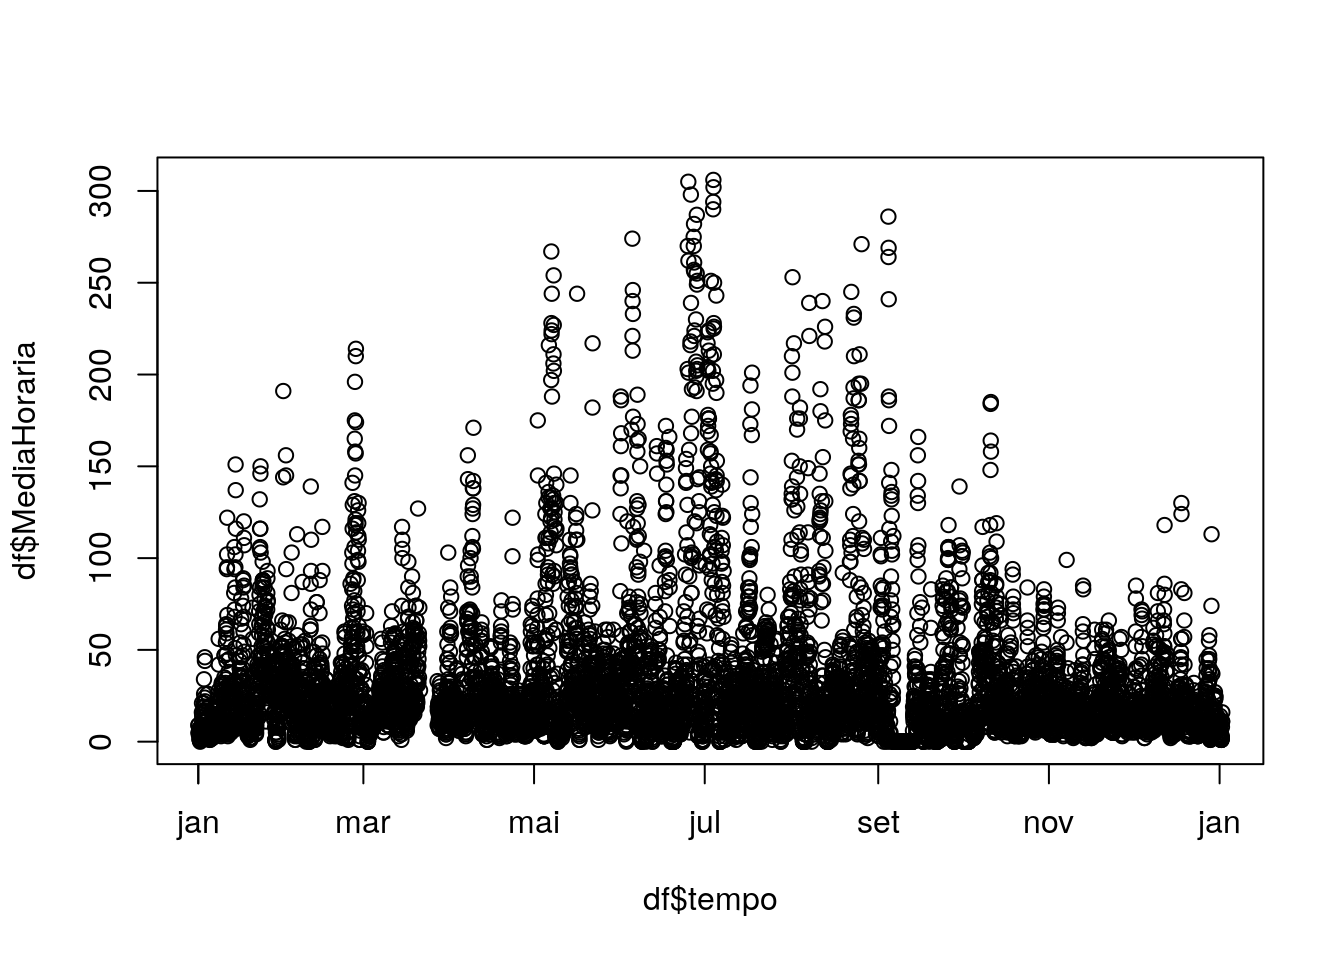
\includegraphics{cursoR_files/figure-latex/unnamed-chunk-68-1.pdf}

feio, ne?

\begin{Shaded}
\begin{Highlighting}[]
\KeywordTok{plot}\NormalTok{(}\DataTypeTok{x =}\NormalTok{ df}\OperatorTok{$}\NormalTok{tempo[}\DecValTok{1}\OperatorTok{:}\DecValTok{100}\NormalTok{], }\DataTypeTok{y =}\NormalTok{ df}\OperatorTok{$}\NormalTok{MediaHoraria[}\DecValTok{1}\OperatorTok{:}\DecValTok{100}\NormalTok{], }
     \DataTypeTok{pch =} \DecValTok{16}\NormalTok{, }\DataTypeTok{type =} \StringTok{"b"}\NormalTok{, }\DataTypeTok{col =} \StringTok{"blue"}\NormalTok{,}
     \DataTypeTok{xlab =} \StringTok{"horas"}\NormalTok{, }\DataTypeTok{ylab =} \StringTok{"NO2[ppb]"}\NormalTok{,}
     \DataTypeTok{main =} \StringTok{"Plot menos feio"}\NormalTok{)}
\end{Highlighting}
\end{Shaded}

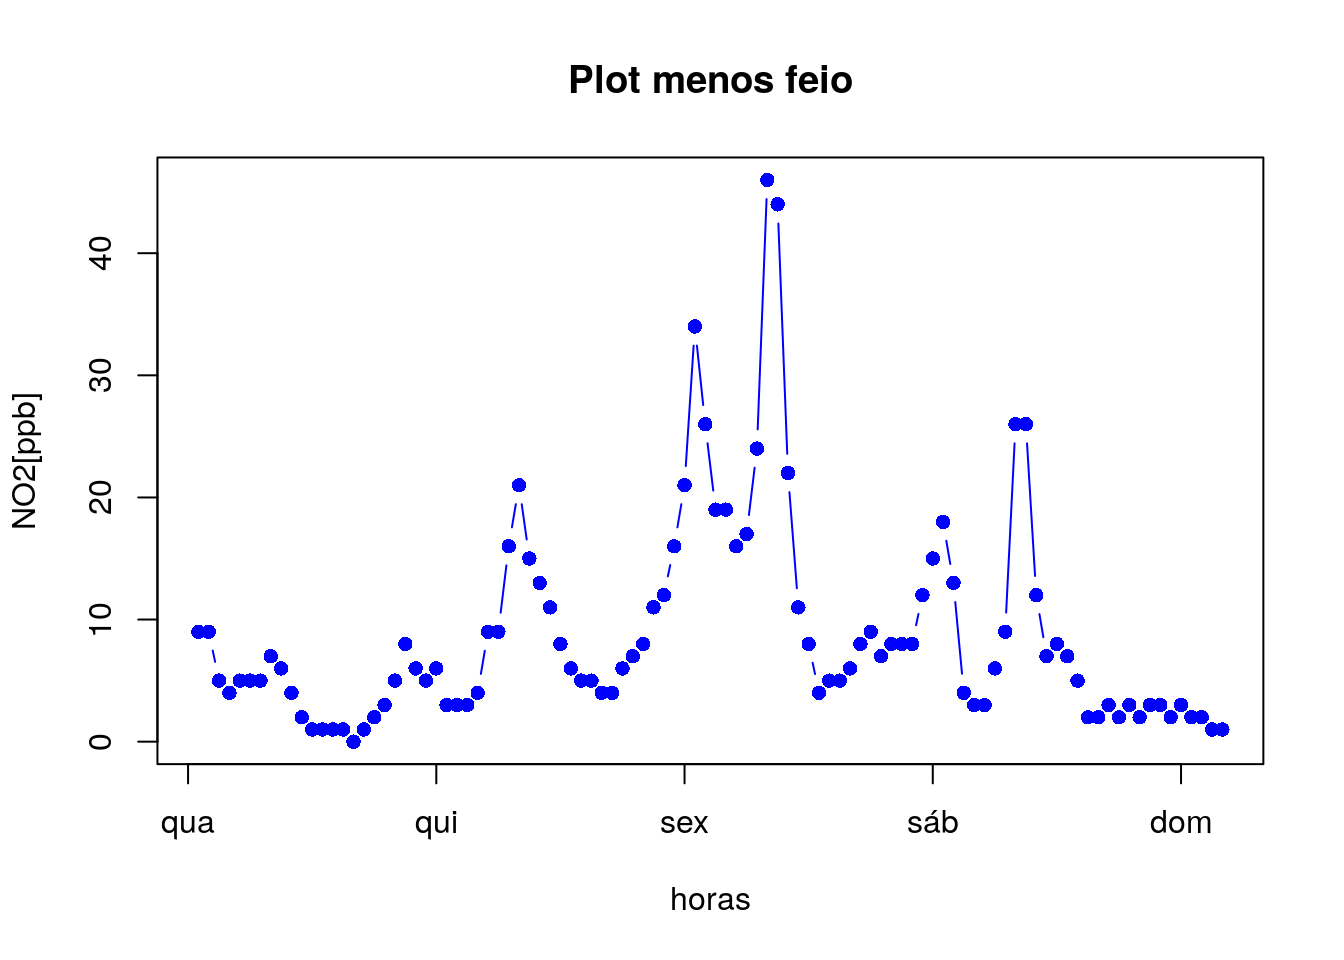
\includegraphics{cursoR_files/figure-latex/unnamed-chunk-69-1.pdf}

Vamos a colocar \textbf{DOIS} plots

\begin{Shaded}
\begin{Highlighting}[]
\KeywordTok{plot}\NormalTok{(}\DataTypeTok{x =}\NormalTok{ df}\OperatorTok{$}\NormalTok{tempo[}\DecValTok{1}\OperatorTok{:}\DecValTok{100}\NormalTok{], }\DataTypeTok{y =}\NormalTok{ df}\OperatorTok{$}\NormalTok{MediaHoraria[}\DecValTok{101}\OperatorTok{:}\DecValTok{200}\NormalTok{], }
     \DataTypeTok{pch =} \DecValTok{16}\NormalTok{, }\DataTypeTok{type =} \StringTok{"b"}\NormalTok{, }\DataTypeTok{col =} \StringTok{"blue"}\NormalTok{,}
     \DataTypeTok{xlab =} \StringTok{"horas"}\NormalTok{, }\DataTypeTok{ylab =} \StringTok{"NO2[ppb]"}\NormalTok{,}
     \DataTypeTok{main =} \StringTok{"Plot estranho"}\NormalTok{)}
\KeywordTok{lines}\NormalTok{(}\DataTypeTok{x =}\NormalTok{ df}\OperatorTok{$}\NormalTok{tempo[}\DecValTok{1}\OperatorTok{:}\DecValTok{100}\NormalTok{], }\DataTypeTok{y =}\NormalTok{ df}\OperatorTok{$}\NormalTok{MediaHoraria[}\DecValTok{1}\OperatorTok{:}\DecValTok{100}\NormalTok{], }
     \DataTypeTok{pch =} \DecValTok{15}\NormalTok{, }\DataTypeTok{type =} \StringTok{"b"}\NormalTok{, }\DataTypeTok{col =} \StringTok{"red"}\NormalTok{)}
\end{Highlighting}
\end{Shaded}

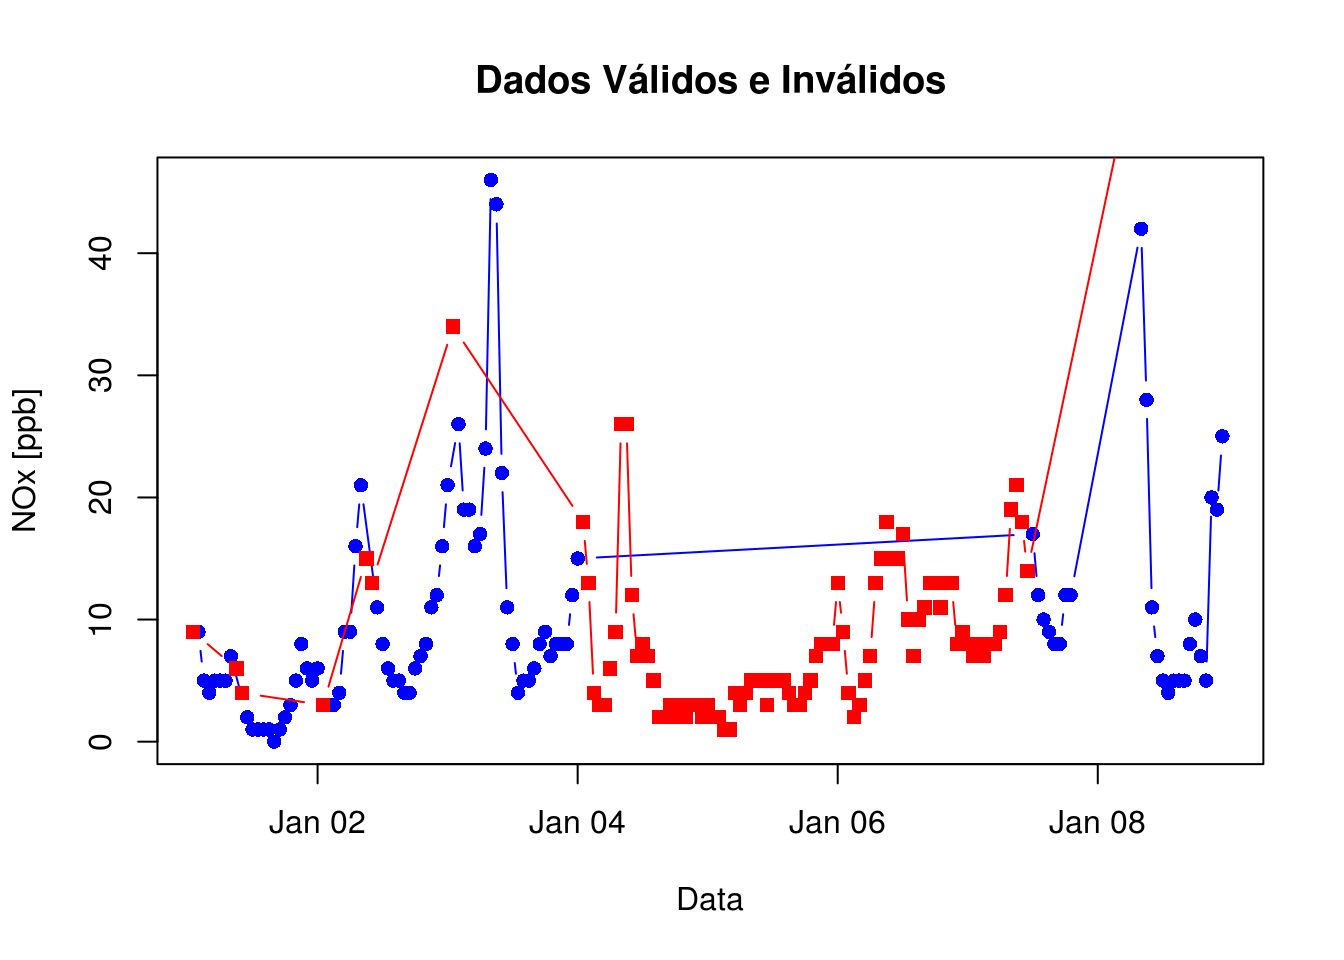
\includegraphics{cursoR_files/figure-latex/unnamed-chunk-70-1.pdf}

Se tu é fan de BASE PLOT, tudo bem :)

\section{ggplot}\label{ggplot}

Tem um monte de recursos para ggplot na web

\begin{Shaded}
\begin{Highlighting}[]
\KeywordTok{library}\NormalTok{(ggplot2)}
\KeywordTok{ggplot}\NormalTok{(df)}
\end{Highlighting}
\end{Shaded}


\includegraphics{cursoR_files/figure-latex/unnamed-chunk-71-1.pdf}

\begin{Shaded}
\begin{Highlighting}[]
\KeywordTok{ggplot}\NormalTok{(df, }\KeywordTok{aes}\NormalTok{(}\DataTypeTok{x =}\NormalTok{ tempo, }\DataTypeTok{y =}\NormalTok{ MediaHoraria))}
\end{Highlighting}
\end{Shaded}

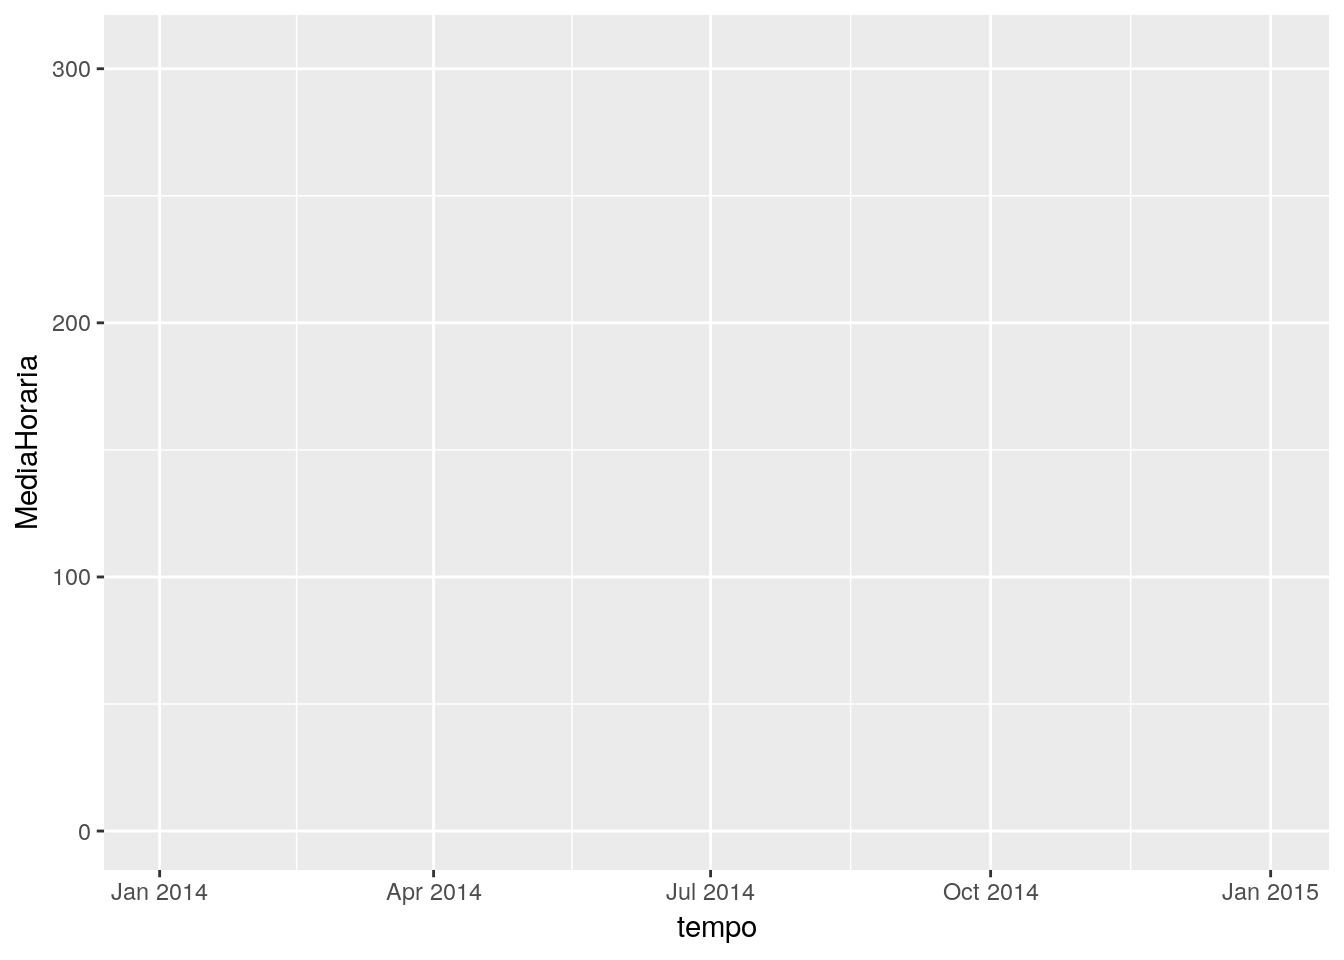
\includegraphics{cursoR_files/figure-latex/unnamed-chunk-72-1.pdf}

\begin{Shaded}
\begin{Highlighting}[]
\KeywordTok{ggplot}\NormalTok{(df, }\KeywordTok{aes}\NormalTok{(}\DataTypeTok{x =}\NormalTok{ tempo, }\DataTypeTok{y =}\NormalTok{ MediaHoraria)) }\OperatorTok{+}\StringTok{ }
\StringTok{  }\KeywordTok{geom_line}\NormalTok{()}
\end{Highlighting}
\end{Shaded}

\begin{verbatim}
## Warning: Removed 1 rows containing missing values (geom_path).
\end{verbatim}

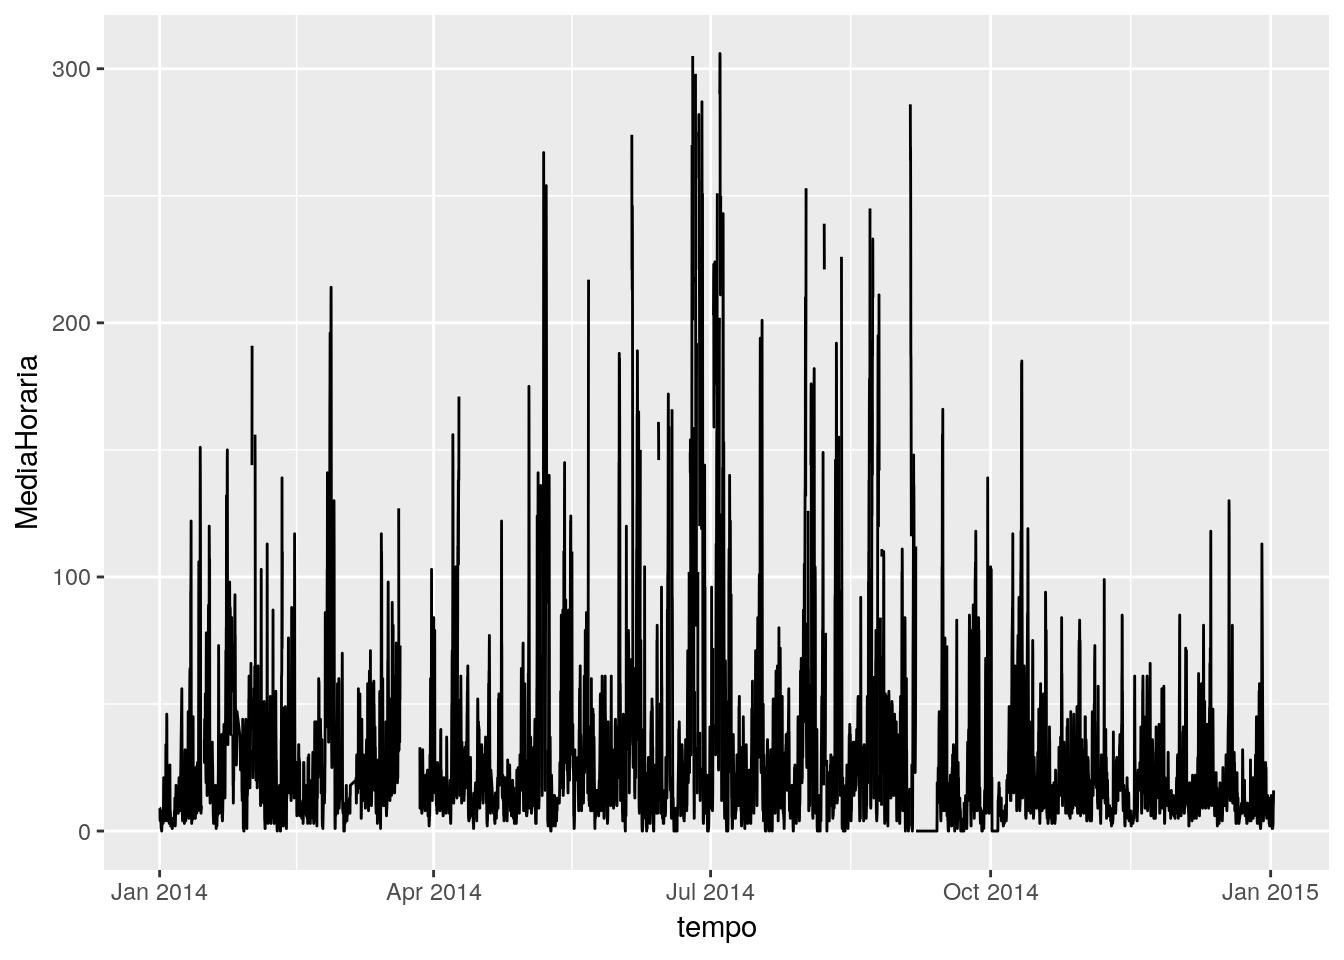
\includegraphics{cursoR_files/figure-latex/unnamed-chunk-73-1.pdf}

opa

\begin{Shaded}
\begin{Highlighting}[]
\KeywordTok{ggplot}\NormalTok{(df, }\KeywordTok{aes}\NormalTok{(}\DataTypeTok{x =}\NormalTok{ tempo, }\DataTypeTok{y =}\NormalTok{ MediaHoraria, }\DataTypeTok{colour =}\NormalTok{ mes)) }\OperatorTok{+}\StringTok{ }
\StringTok{  }\KeywordTok{geom_line}\NormalTok{() }
\end{Highlighting}
\end{Shaded}

\begin{verbatim}
## Warning: Removed 1 rows containing missing values (geom_path).
\end{verbatim}

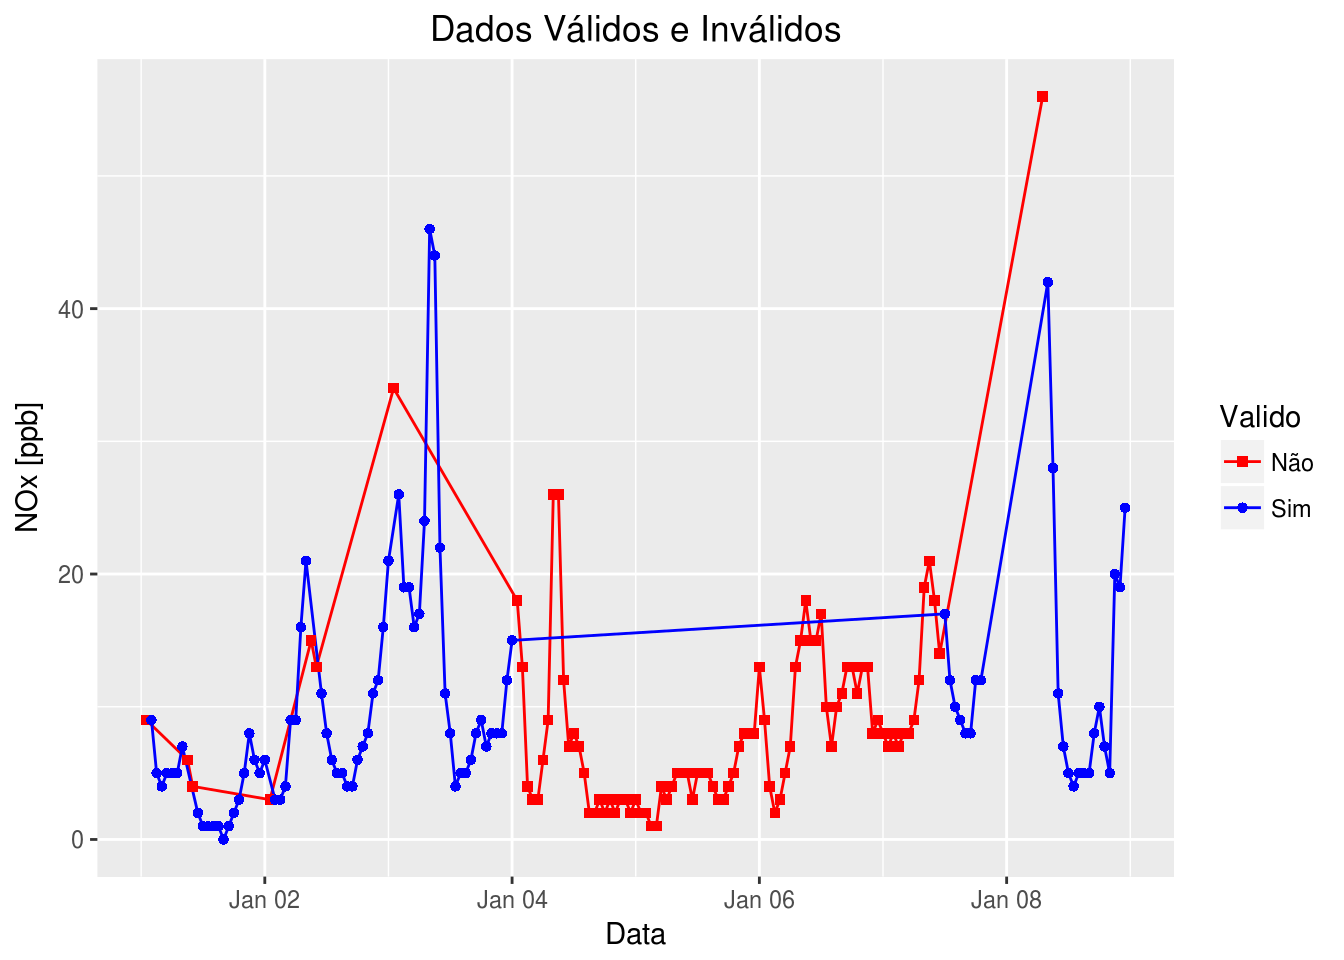
\includegraphics{cursoR_files/figure-latex/unnamed-chunk-74-1.pdf}

deixando so 2014

\begin{Shaded}
\begin{Highlighting}[]
\NormalTok{df <-}\StringTok{ }\NormalTok{df[df}\OperatorTok{$}\NormalTok{ano }\OperatorTok{==}\StringTok{ }\DecValTok{2014}\NormalTok{,]}
\end{Highlighting}
\end{Shaded}

\begin{Shaded}
\begin{Highlighting}[]
\KeywordTok{ggplot}\NormalTok{(df, }\KeywordTok{aes}\NormalTok{(}\DataTypeTok{x =}\NormalTok{ tempo, }\DataTypeTok{y =}\NormalTok{ MediaHoraria, }\DataTypeTok{colour =}\NormalTok{ mes)) }\OperatorTok{+}\StringTok{ }
\StringTok{  }\KeywordTok{geom_line}\NormalTok{() }\OperatorTok{+}
\StringTok{  }\KeywordTok{theme_bw}\NormalTok{()}
\end{Highlighting}
\end{Shaded}

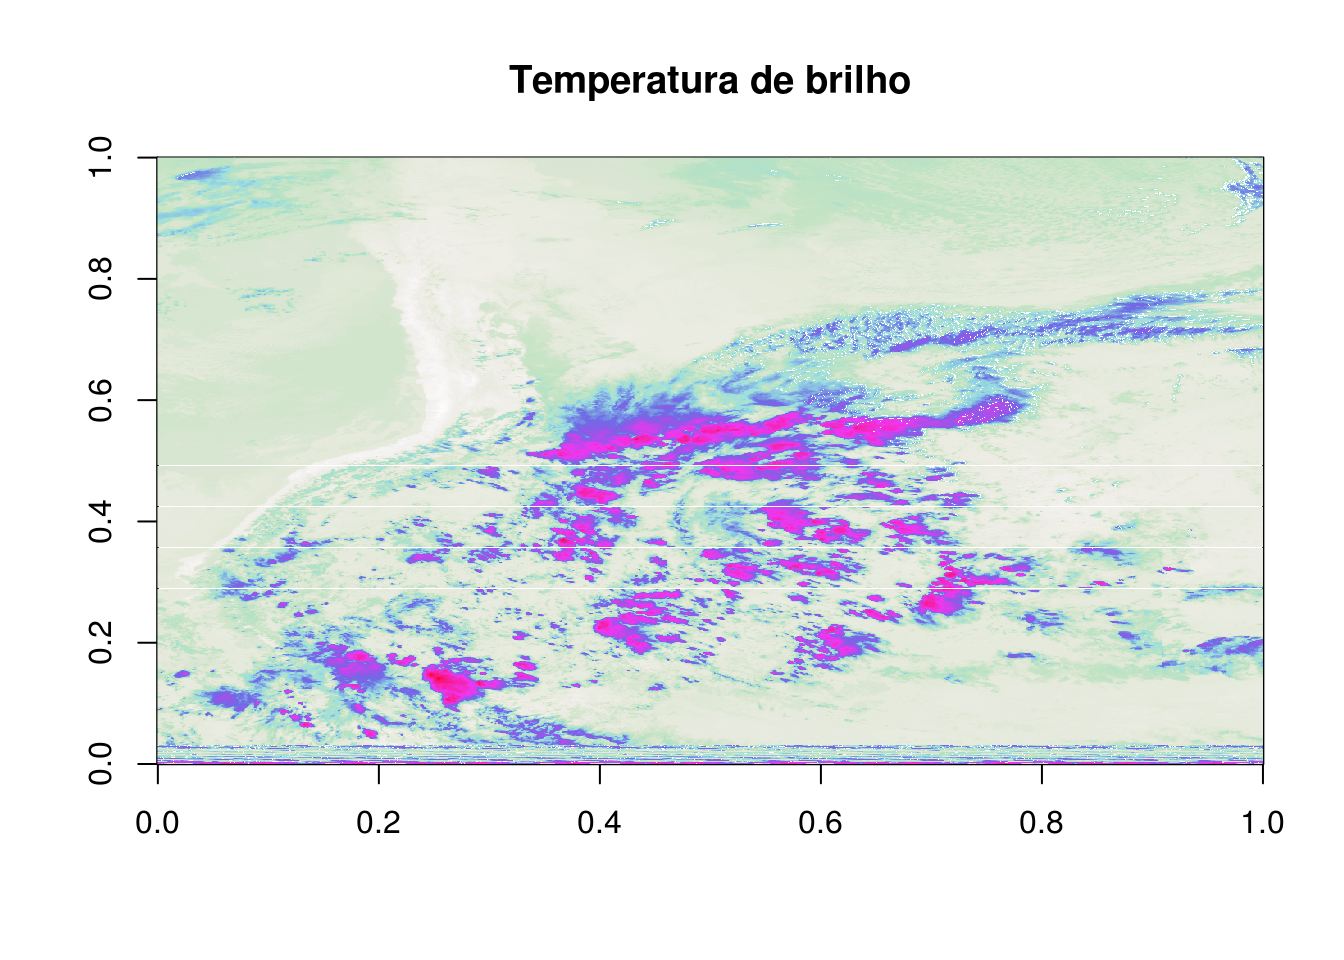
\includegraphics{cursoR_files/figure-latex/unnamed-chunk-76-1.pdf}

\begin{Shaded}
\begin{Highlighting}[]
\KeywordTok{ggplot}\NormalTok{(df, }\KeywordTok{aes}\NormalTok{(}\DataTypeTok{x =}\NormalTok{ tempo, }\DataTypeTok{y =}\NormalTok{ MediaHoraria, }\DataTypeTok{colour =}\NormalTok{ MediaHoraria)) }\OperatorTok{+}\StringTok{ }
\StringTok{  }\KeywordTok{geom_line}\NormalTok{() }
\end{Highlighting}
\end{Shaded}

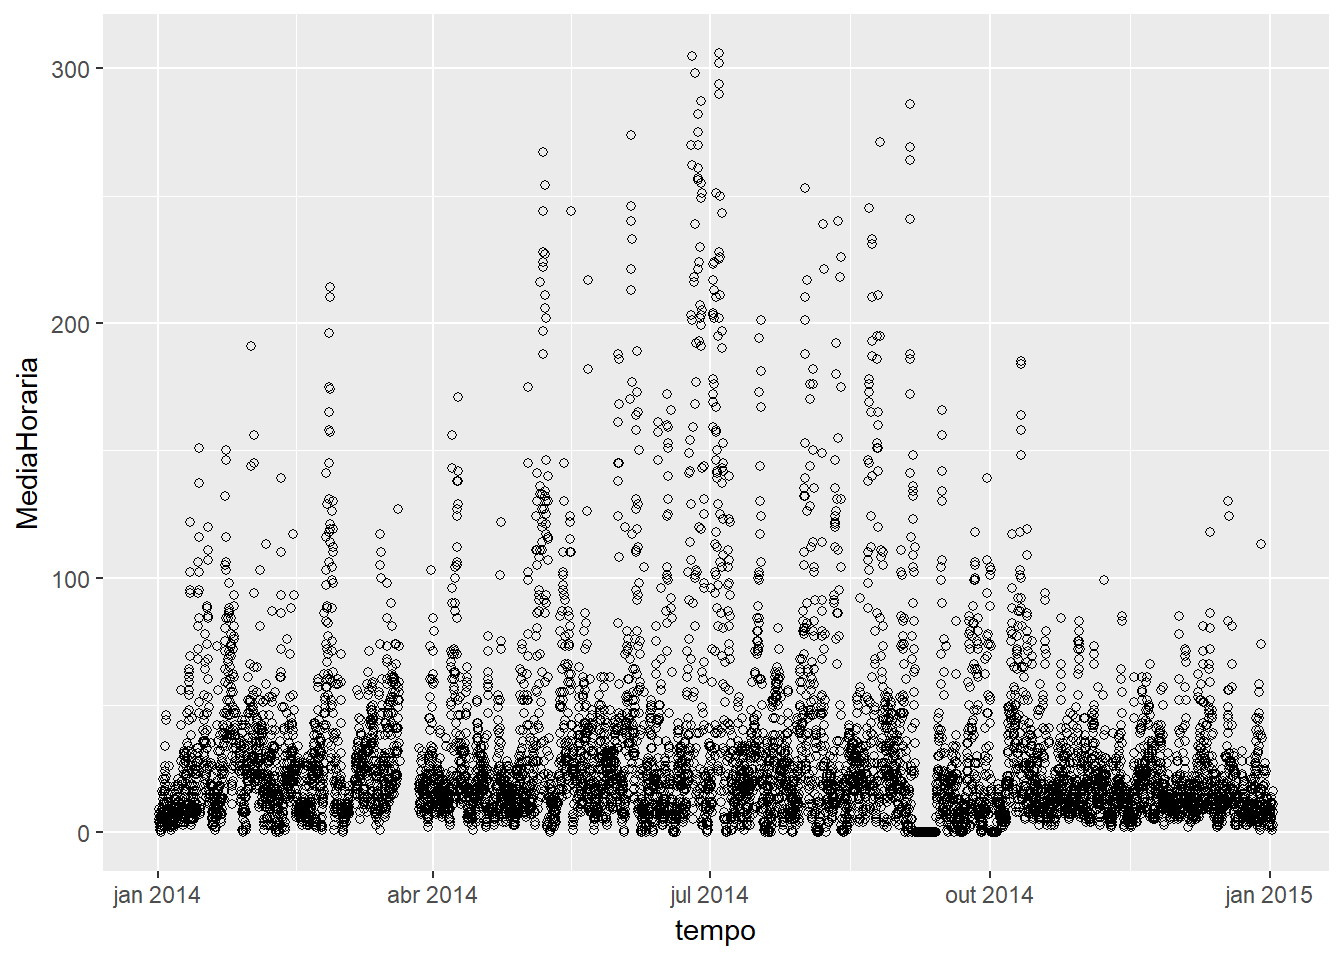
\includegraphics{cursoR_files/figure-latex/unnamed-chunk-77-1.pdf}

\begin{Shaded}
\begin{Highlighting}[]
\KeywordTok{ggplot}\NormalTok{(df, }\KeywordTok{aes}\NormalTok{(}\DataTypeTok{x =}\NormalTok{ tempo, }\DataTypeTok{y =}\NormalTok{ MediaHoraria, }\DataTypeTok{colour =}\NormalTok{ MediaHoraria)) }\OperatorTok{+}\StringTok{ }
\StringTok{  }\KeywordTok{geom_line}\NormalTok{() }\OperatorTok{+}
\StringTok{  }\KeywordTok{facet_wrap}\NormalTok{(}\OperatorTok{~}\NormalTok{mes)}
\end{Highlighting}
\end{Shaded}

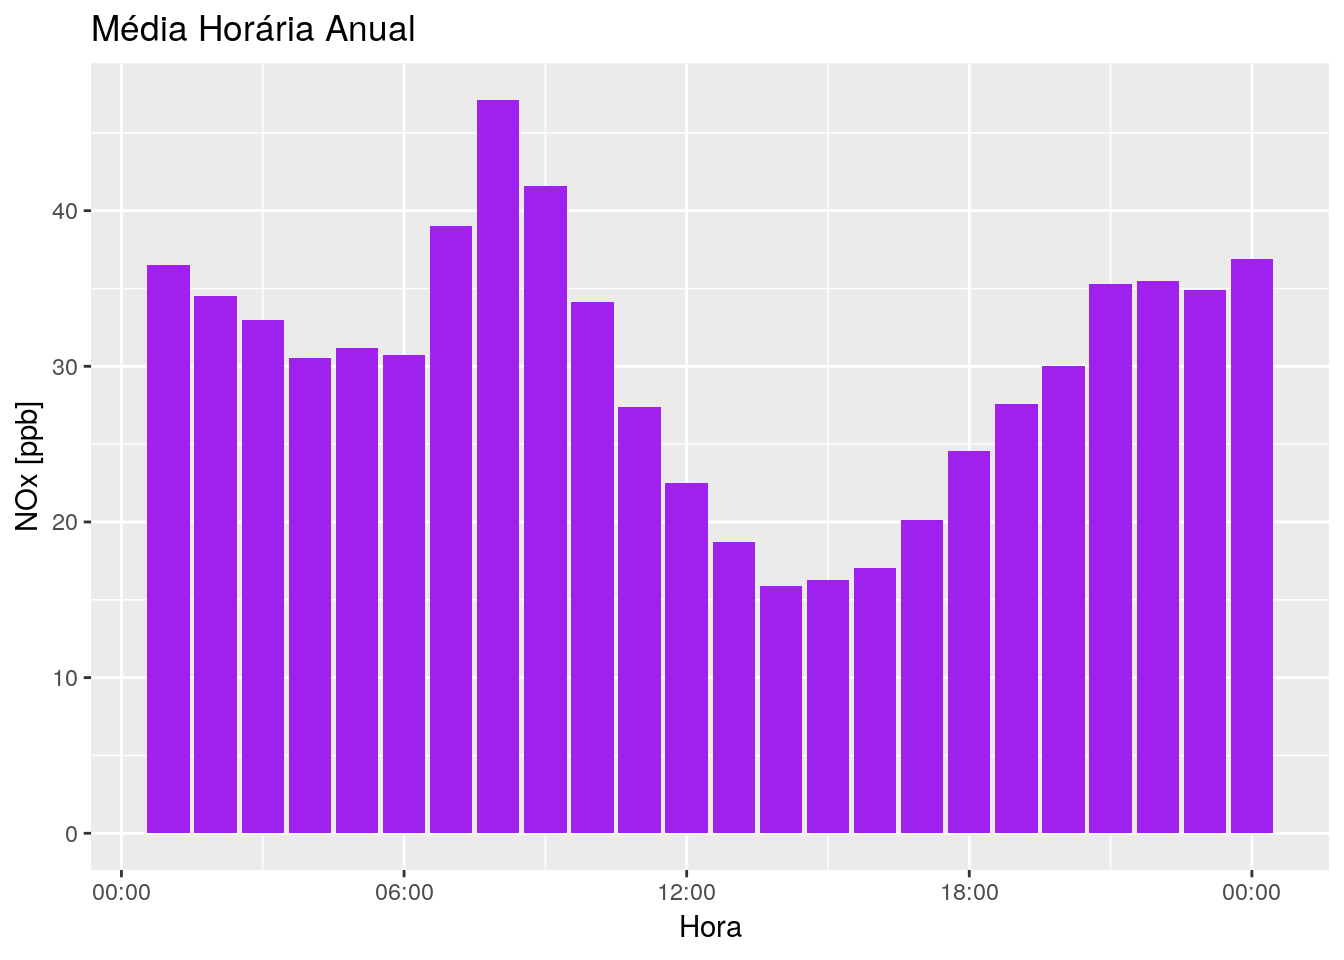
\includegraphics{cursoR_files/figure-latex/unnamed-chunk-78-1.pdf}

\begin{Shaded}
\begin{Highlighting}[]
\KeywordTok{ggplot}\NormalTok{(df, }\KeywordTok{aes}\NormalTok{(}\DataTypeTok{x =}\NormalTok{ tempo, }\DataTypeTok{y =}\NormalTok{ MediaHoraria, }\DataTypeTok{colour =}\NormalTok{ MediaHoraria)) }\OperatorTok{+}\StringTok{ }
\StringTok{  }\KeywordTok{geom_line}\NormalTok{() }\OperatorTok{+}
\StringTok{  }\KeywordTok{facet_wrap}\NormalTok{(}\OperatorTok{~}\NormalTok{mes, }\DataTypeTok{scales =} \StringTok{"free"}\NormalTok{)}
\end{Highlighting}
\end{Shaded}

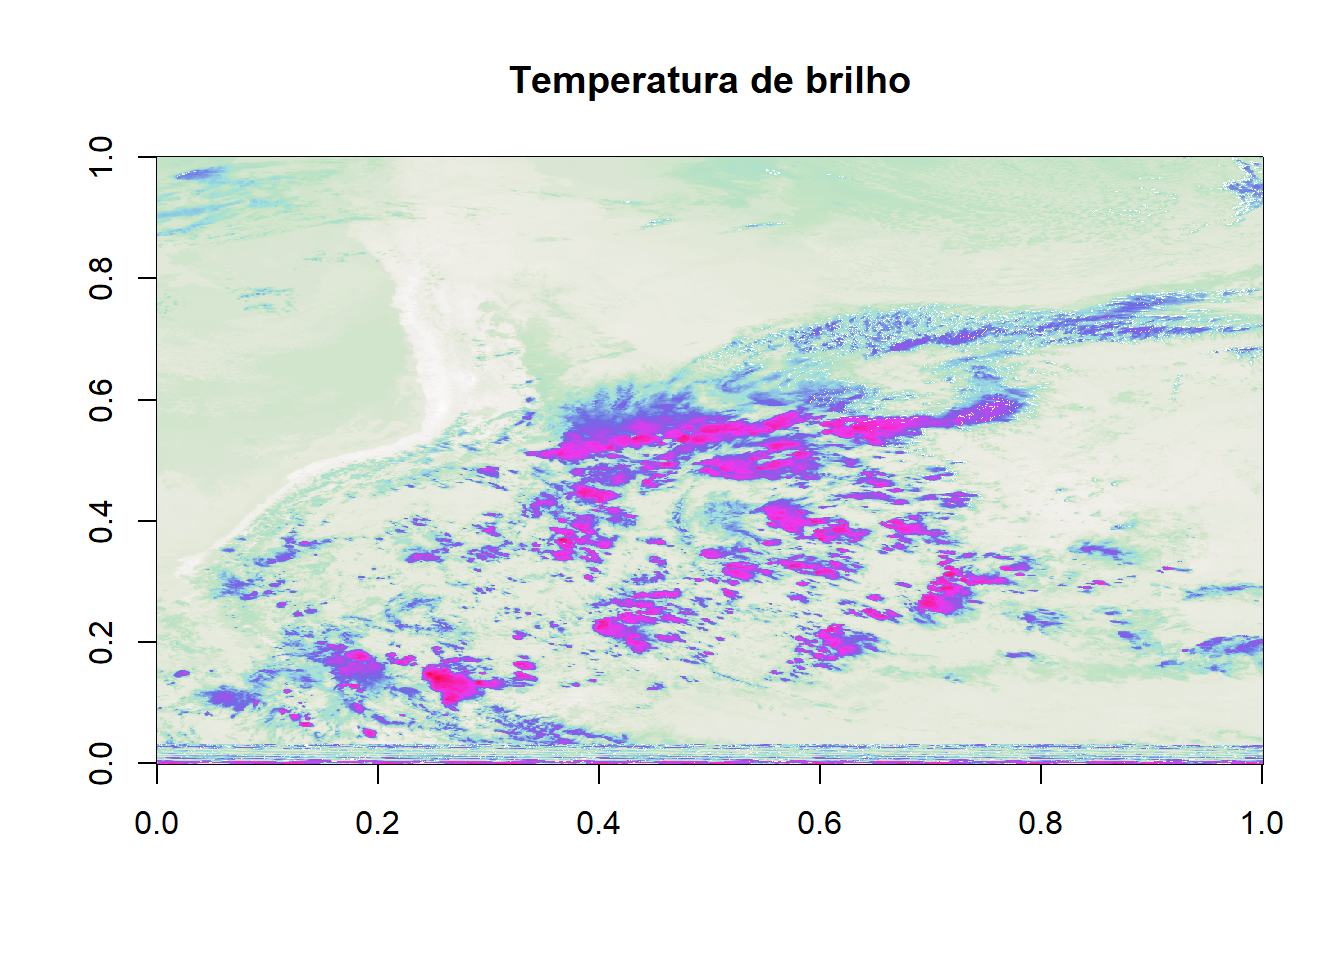
\includegraphics{cursoR_files/figure-latex/unnamed-chunk-79-1.pdf}

Y para terminar, meu theme favorito

\begin{Shaded}
\begin{Highlighting}[]
\NormalTok{devtools}\OperatorTok{::}\KeywordTok{install_github}\NormalTok{(}\StringTok{"atmoschem/veinreport"}\NormalTok{)}
\end{Highlighting}
\end{Shaded}

e logo

\begin{Shaded}
\begin{Highlighting}[]
\KeywordTok{library}\NormalTok{(veinreport)}
\KeywordTok{library}\NormalTok{(cptcity)}
\end{Highlighting}
\end{Shaded}

\begin{Shaded}
\begin{Highlighting}[]
\KeywordTok{ggplot}\NormalTok{(df, }\KeywordTok{aes}\NormalTok{(}\DataTypeTok{x =}\NormalTok{ tempo, }\DataTypeTok{y =}\NormalTok{ MediaHoraria, }\DataTypeTok{colour =}\NormalTok{ MediaHoraria)) }\OperatorTok{+}\StringTok{ }
\StringTok{  }\KeywordTok{geom_line}\NormalTok{()}\OperatorTok{+}
\StringTok{  }\KeywordTok{theme_black}\NormalTok{() }\OperatorTok{+}
\StringTok{  }\KeywordTok{scale_color_gradientn}\NormalTok{(}\DataTypeTok{colours =} \KeywordTok{cpt}\NormalTok{())}
\end{Highlighting}
\end{Shaded}

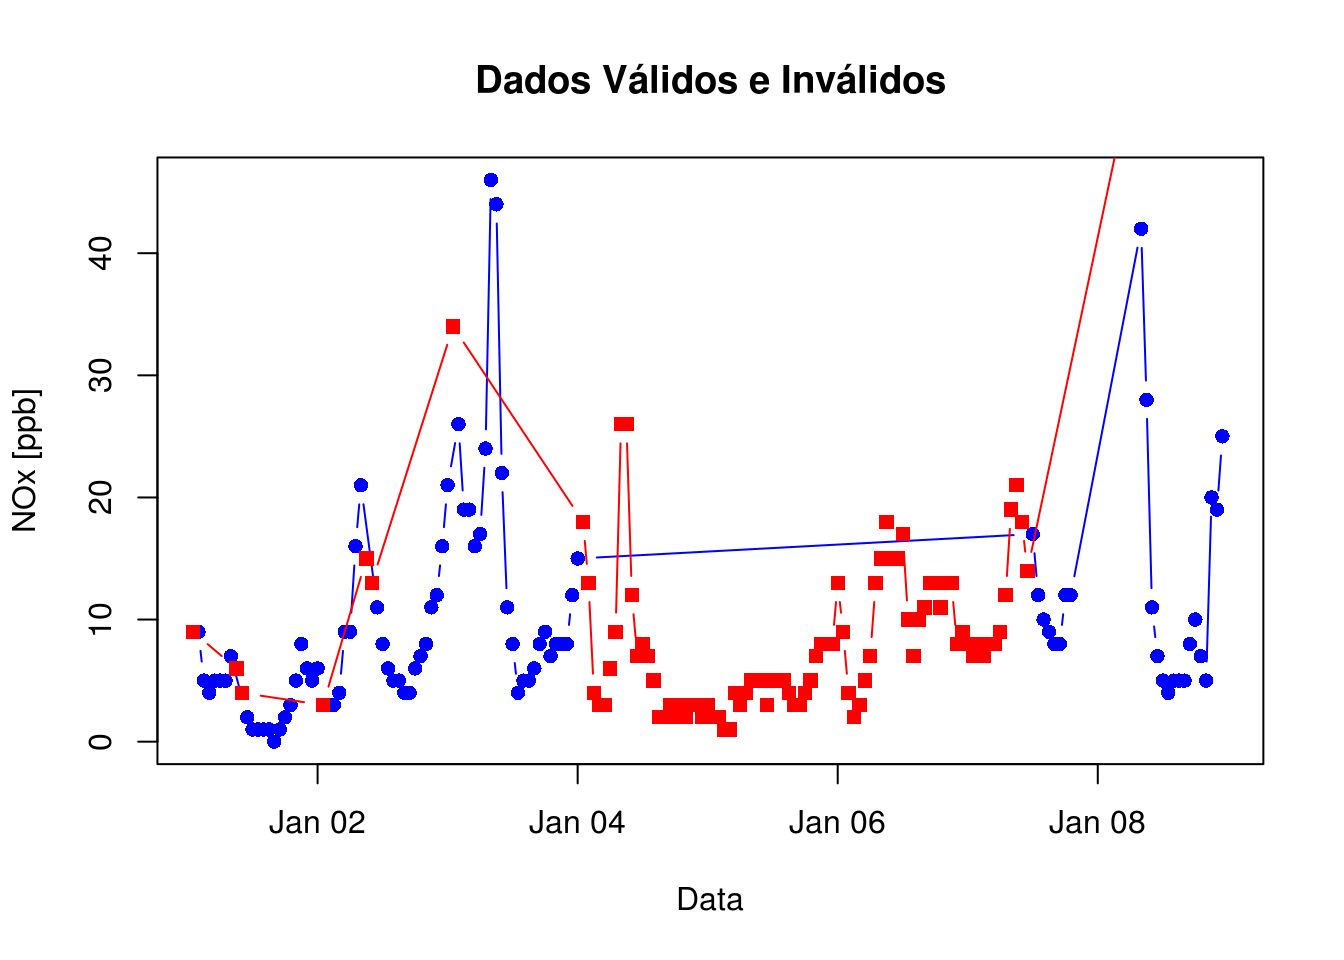
\includegraphics{cursoR_files/figure-latex/unnamed-chunk-82-1.pdf}

Pode revertir a escala de cores

\begin{Shaded}
\begin{Highlighting}[]
\KeywordTok{ggplot}\NormalTok{(df, }\KeywordTok{aes}\NormalTok{(}\DataTypeTok{x =}\NormalTok{ tempo, }\DataTypeTok{y =}\NormalTok{ MediaHoraria, }\DataTypeTok{colour =}\NormalTok{ MediaHoraria)) }\OperatorTok{+}\StringTok{ }
\StringTok{  }\KeywordTok{geom_line}\NormalTok{()}\OperatorTok{+}
\StringTok{  }\KeywordTok{theme_black}\NormalTok{() }\OperatorTok{+}
\StringTok{  }\KeywordTok{scale_color_gradientn}\NormalTok{(}\DataTypeTok{colours =} \KeywordTok{rev}\NormalTok{(}\KeywordTok{cpt}\NormalTok{())) }\OperatorTok{+}\StringTok{ }
\StringTok{  }\KeywordTok{facet_wrap}\NormalTok{(}\OperatorTok{~}\NormalTok{mes, }\DataTypeTok{scales =} \StringTok{"free"}\NormalTok{)}
\end{Highlighting}
\end{Shaded}

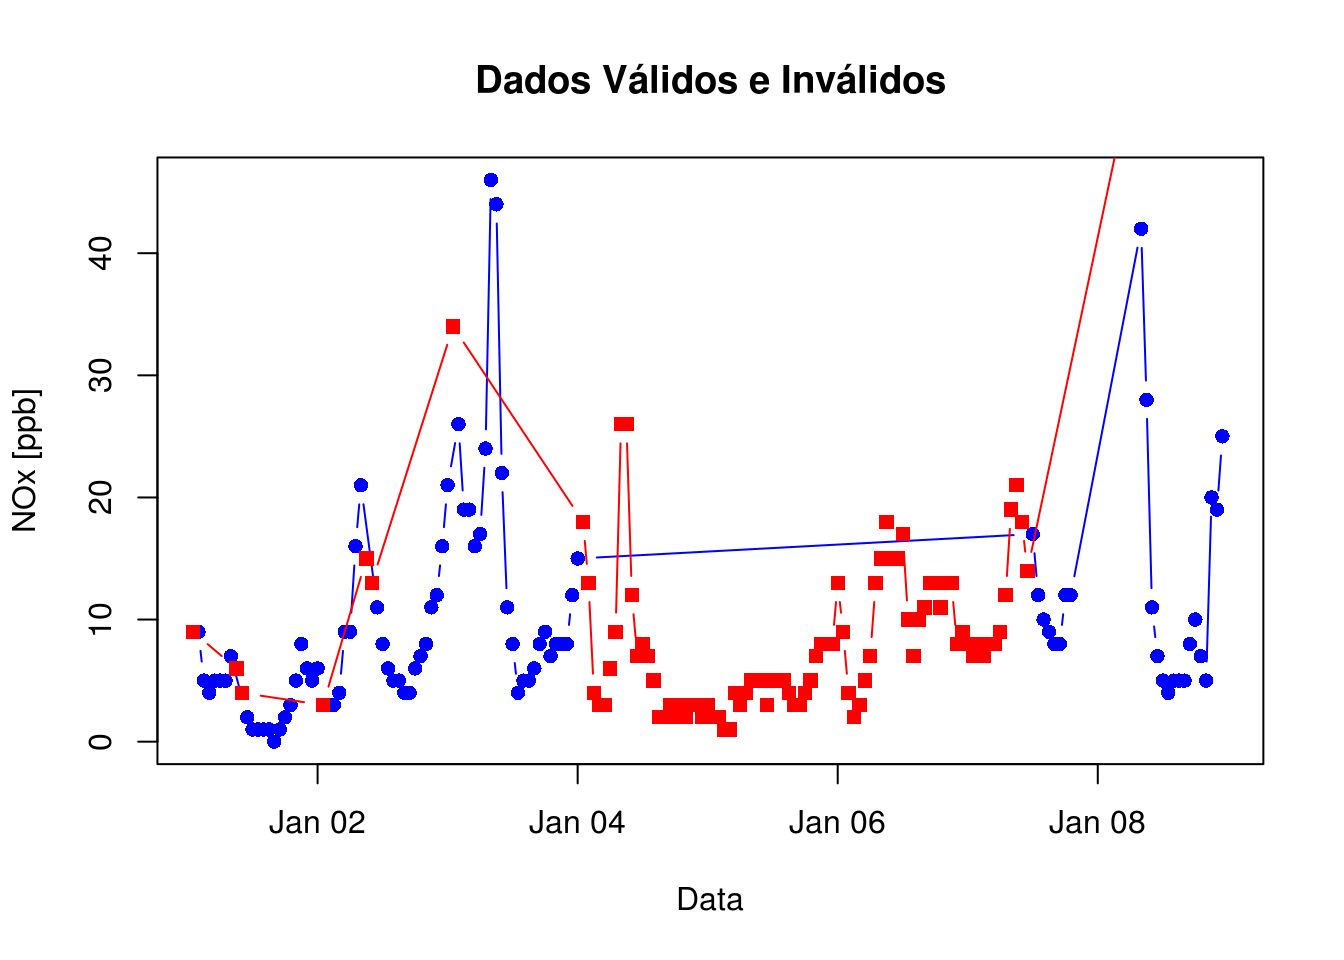
\includegraphics{cursoR_files/figure-latex/unnamed-chunk-83-1.pdf}

não gostou, tenta com a sorte

\begin{Shaded}
\begin{Highlighting}[]
\KeywordTok{ggplot}\NormalTok{(df, }\KeywordTok{aes}\NormalTok{(}\DataTypeTok{x =}\NormalTok{ tempo, }\DataTypeTok{y =}\NormalTok{ MediaHoraria, }\DataTypeTok{colour =}\NormalTok{ MediaHoraria)) }\OperatorTok{+}\StringTok{ }
\StringTok{  }\KeywordTok{geom_line}\NormalTok{()}\OperatorTok{+}
\StringTok{  }\KeywordTok{theme_black}\NormalTok{() }\OperatorTok{+}
\StringTok{    }\KeywordTok{facet_wrap}\NormalTok{(}\OperatorTok{~}\NormalTok{mes, }\DataTypeTok{scales =} \StringTok{"free"}\NormalTok{) }\OperatorTok{+}
\StringTok{  }\KeywordTok{scale_color_gradientn}\NormalTok{(}\DataTypeTok{colours =} \KeywordTok{lucky}\NormalTok{())}
\end{Highlighting}
\end{Shaded}

\begin{verbatim}
## Colour gradient: gacruxa_fib54_fib54_04, number: 2398
\end{verbatim}

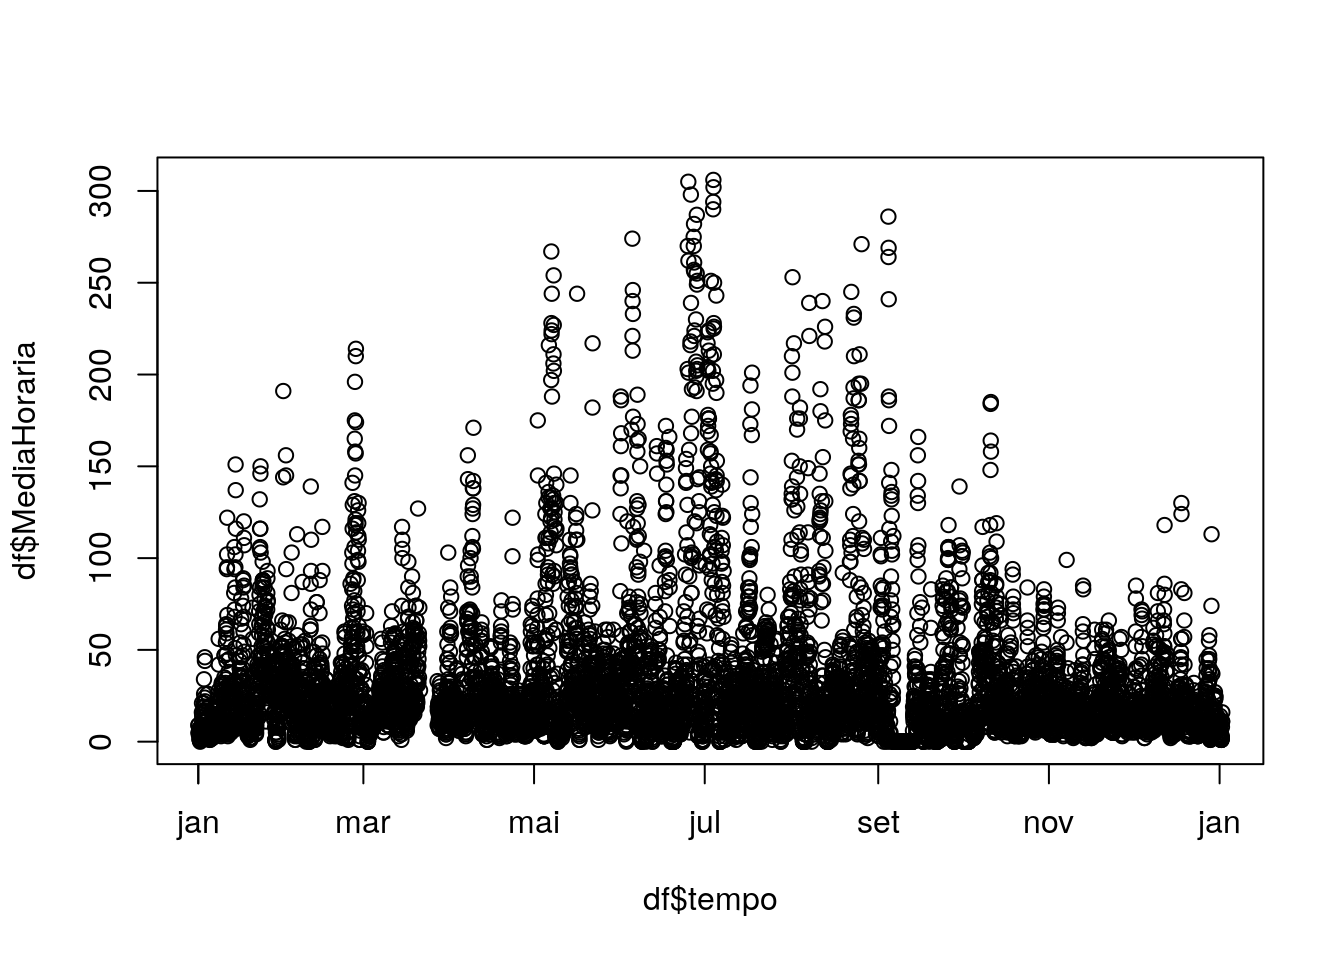
\includegraphics{cursoR_files/figure-latex/unnamed-chunk-84-1.pdf}

\begin{Shaded}
\begin{Highlighting}[]
\KeywordTok{ggplot}\NormalTok{(df, }\KeywordTok{aes}\NormalTok{(}\DataTypeTok{x =}\NormalTok{ tempo, }\DataTypeTok{y =}\NormalTok{ MediaHoraria, }\DataTypeTok{colour =}\NormalTok{ MediaHoraria)) }\OperatorTok{+}\StringTok{ }
\StringTok{  }\KeywordTok{geom_line}\NormalTok{()}\OperatorTok{+}
\StringTok{  }\KeywordTok{theme_black}\NormalTok{() }\OperatorTok{+}
\StringTok{    }\KeywordTok{facet_wrap}\NormalTok{(}\OperatorTok{~}\NormalTok{mes, }\DataTypeTok{scales =} \StringTok{"free"}\NormalTok{) }\OperatorTok{+}
\StringTok{  }\KeywordTok{scale_color_gradientn}\NormalTok{(}\DataTypeTok{colours =} \KeywordTok{lucky}\NormalTok{())}
\end{Highlighting}
\end{Shaded}

\begin{verbatim}
## Colour gradient: ing_xmas_ib_jul17, number: 3612
\end{verbatim}

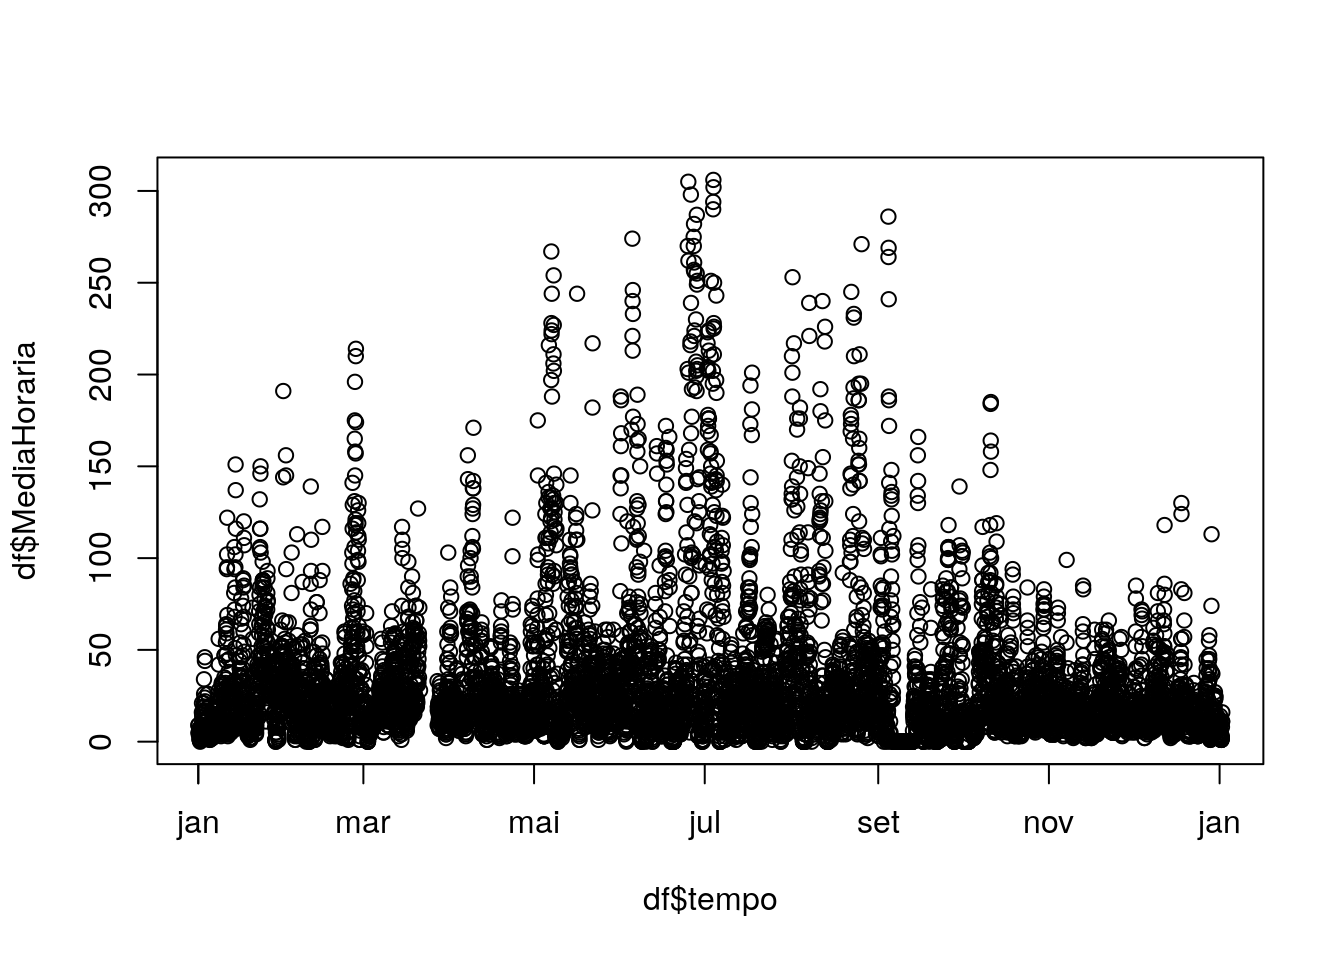
\includegraphics{cursoR_files/figure-latex/unnamed-chunk-85-1.pdf}

\begin{Shaded}
\begin{Highlighting}[]
\KeywordTok{ggplot}\NormalTok{(df, }\KeywordTok{aes}\NormalTok{(}\DataTypeTok{x =}\NormalTok{ tempo, }\DataTypeTok{y =}\NormalTok{ MediaHoraria, }\DataTypeTok{colour =}\NormalTok{ MediaHoraria)) }\OperatorTok{+}\StringTok{ }
\StringTok{  }\KeywordTok{geom_line}\NormalTok{()}\OperatorTok{+}
\StringTok{  }\KeywordTok{theme_black}\NormalTok{() }\OperatorTok{+}
\StringTok{  }\KeywordTok{scale_color_gradientn}\NormalTok{(}\DataTypeTok{colours =} \KeywordTok{lucky}\NormalTok{())}
\end{Highlighting}
\end{Shaded}

\begin{verbatim}
## Colour gradient: es_ocean_breeze_es_ocean_breeze_130, number: 1632
\end{verbatim}

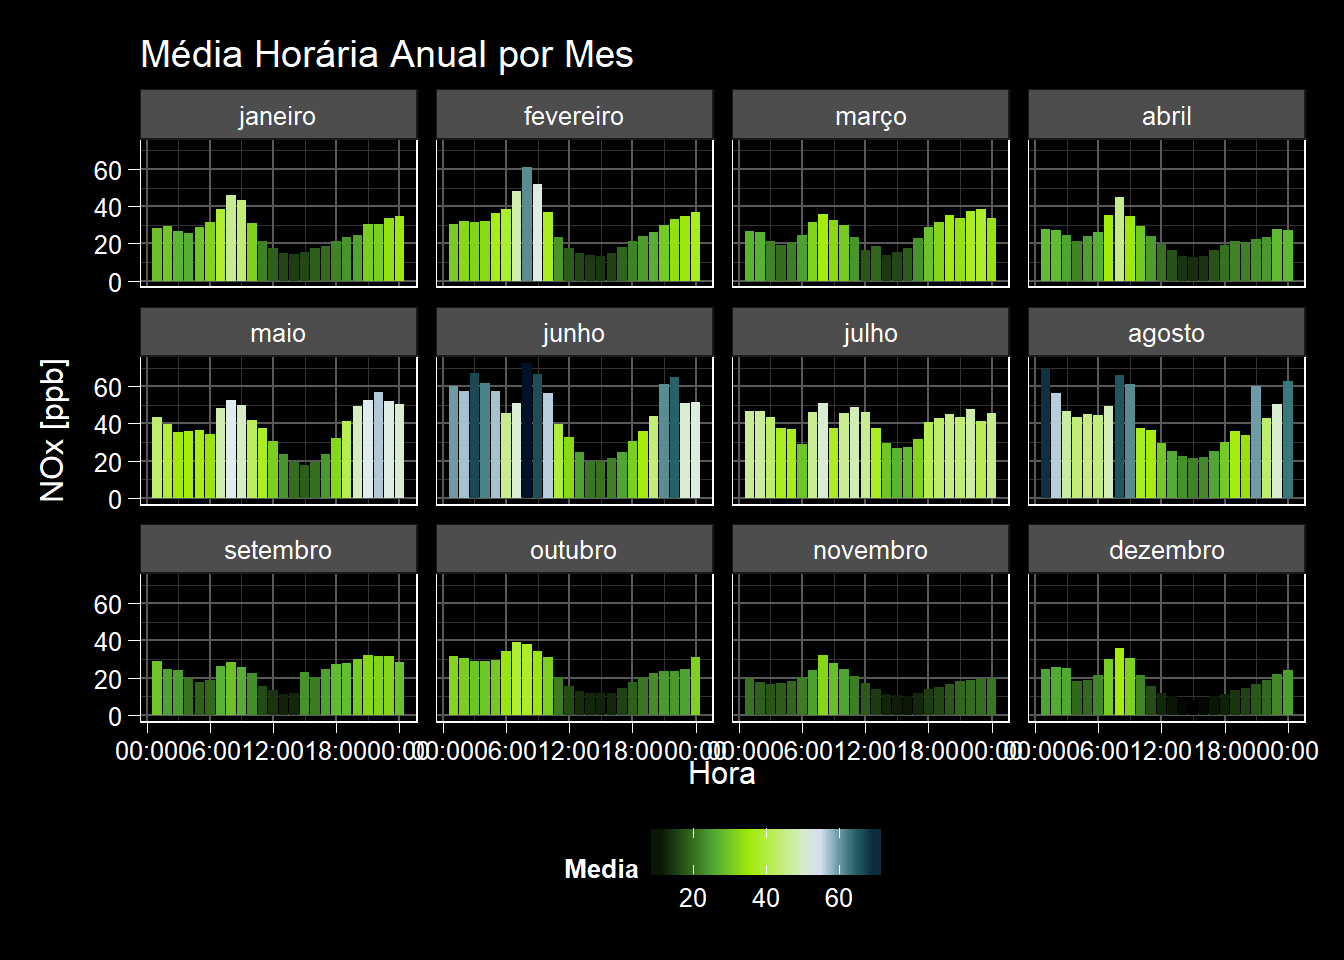
\includegraphics{cursoR_files/figure-latex/unnamed-chunk-86-1.pdf}

\chapter{\texorpdfstring{Geo Spatial: \texttt{raster}, \texttt{sf} e
\texttt{stars}}{Geo Spatial: raster, sf e stars}}\label{geo-spatial-raster-sf-e-stars}

Coming soon

\bibliography{book.bib,packages.bib}


\end{document}
